\documentclass[twoside,english]{uiofysmaster/uiofysmaster}

\usepackage[toc,titletoc,title,page]{appendix} %to add appendices (and have them in toc)
\usepackage[utf8]{inputenc}
%\usepackage{mhchem} %latex chemistry symbols
\usepackage{blindtext} %to fill in dummy text
%\usepackage{cite} %to have multiple citations in one \cite{key1,key2,..} -do not use with natbib!!
\usepackage{tcolorbox} %to have boxes w color around text and math mode
\usepackage{enumitem} %to reduce vertical spacing in enumerate
\usepackage{tabu} % to set tables to page width
%\usepackage{aas_macros}

\usepackage[sort&compress,square,comma,numbers]{natbib} %to use \citet, now mixed with [nr]
\usepackage[nottoc]{tocbibind}

\usepackage{float} 
\usepackage[export]{adjustbox}
\usepackage{subcaption}
\newcommand{\blank}[1]{\hspace*{#1}} % move figures by \blank{}
\usepackage{pdfpages}
\usepackage{tikz}
\usetikzlibrary{
	arrows, 
	shapes.callouts,
	decorations.pathreplacing,
	decorations.pathmorphing,
	calc
}
\usepackage{stackengine}
\usepackage{revsymb} % used for lambda-bar

%---

\interfootnotelinepenalty=10000 % to force footnotes to NOT run over to the next page

%---
% to reduce space around table of contents (to fit everything into one page): 
\usepackage{tocloft}
\setlength{\cftbeforetoctitleskip}{0pt}
\setlength{\cftaftertoctitleskip}{0pt}
%---

\usepackage{epigraph}
\setlength\epigraphwidth{11cm}
\setlength\epigraphrule{0pt}

%---
\newcommand{\Sm}{$^{140}$Sm} % making it faster to write Sm140
\newcommand{\Pb}{$^{208}$Pb} 
\newcommand{\bd}{$\beta$-decay} % making it faster to write 
\newcommand{\ga}{$\gamma$}
\newcommand{\MBOU}{MAR\belowbaseline[-2pt]{a}B\stackinset{l}{3pt}{b}{-3pt}{O}{O}\,U}
\newcommand{\Ba}{$^{133}$Ba}
\newcommand{\Eu}{$^{152}$Eu}

%---
% modifying color in code listings and some style
%\usepackage{color}

% The predefined color names are: 
% black, blue, brown, cyan, darkgray, gray, green, lightgray, lime, magenta, olive, orange, pink, purple, red, teal, violet, white, yellow.
 
%\definecolor{codegreen}{rgb}{0,0.6,0} % too flashy
\definecolor{codegreen}{rgb}{0.0, 0.42, 0.24} % less flashy so comments not take all attention
\definecolor{codegray}{rgb}{0.5,0.5,0.5}
\definecolor{codepurple}{rgb}{0.58,0,0.82}
%\definecolor{codepurple}{rgb}{1.0, 0.0, 0.22} %carminered, could try it 
%\definecolor{backcolour}{rgb}{0.95,0.95,0.92} % original suggestion
\definecolor{backcolour}{rgb}{0.94, 0.97, 1.0}% aliceblue, not so flashy and not as ugly
\definecolor{LightGray}{gray}{0.95}
 
\lstdefinestyle{mystyle}{
    backgroundcolor=\color{backcolour},   
    commentstyle=\color{codegreen},
    %commentstyle=\color{codegray},    
    keywordstyle=\color{magenta},
    numberstyle=\tiny\color{codegray},
    stringstyle=\color{codepurple},
    basicstyle=\footnotesize,
    breakatwhitespace=false,         
    breaklines=true,                 
    captionpos=b,                    
    keepspaces=true,                 
    %numbers=left,     %removing line numbers in the code snippets               
    %numbersep=5pt,                  
    showspaces=false,                
    showstringspaces=false,
    showtabs=false,                  
    tabsize=2,
    %float=tp,
    %floatplacement=tbp
}
 
\lstset{
	style=mystyle,
	literate={~} {$\sim$}{1}
}
\renewcommand{\lstlistingname}{Code}
%---

%---
% new tcolorbox environment
% #1: tcolorbox options
% #2: color
% #3: box title
\newtcolorbox{mybox}[3][]
{
  colframe = #2!25,
  colback  = #2!10,
  coltitle = #2!20!black,  
  title    = #3,
  #1,
}

%% Source: http://www.tedpavlic.com/post_preamble_for_journal_of_math_bio.php
%% We need to redefine \autoref. We should use 
%% abbreviations inside the sentence and full names 
%% at the beginning of sentences. Additionally,
%% need to handle the plural cases.

\newcommand*{\Appendixautorefname}{Appendix} % Add Appendix to \autoref 

% \Autoref is for the beginning of the sentence
%\let\orgautoref\autoref
%\providecommand{\Autoref}
%        {\def\equationautorefname{Equation}%
%         \def\figureautorefname{Figure}%
%         \def\subfigureautorefname{Figure}%
%         \def\sectionautorefname{Section}%
%         \def\subsectionautorefname{Section}%
%         \def\subsubsectionautorefname{Section}%
%         \def\Itemautorefname{Item}%
%         \def\tableautorefname{Table}%
%         \orgautoref}

% \Autorefs is plural for the beginning of the sentence
%\providecommand{\Autorefs}
%        {\def\equationautorefname{Equations}%
%         \def\figureautorefname{Figures}%
%         \def\subfigureautorefname{Figures}%
%         \def\sectionautorefname{Sections}%
%         \def\subsectionautorefname{Sections}%
%         \def\subsubsectionautorefname{Sections}%
%         \def\Itemautorefname{Items}%
%         \def\tableautorefname{Tables}%
%         \orgautoref}

% \autoref is used inside a sentence 
% (this is a renew of the standard)
% OBS! Note the "%" at the end of all lines. This is to prevent a leading space when using autoref.
\let\orgautoref\autoref
\renewcommand{\autoref}
        {%\def\equationautorefname{Eq.}%
		 %\def\figureautorefname{Fig.}%
	  	 % \def\subfigureautorefname{Fig.}%
		 \def\sectionautorefname{Section}% % \def\sectionautorefname{Sec.}%
		 \def\subsectionautorefname{Section}% % \def\subsectionautorefname{Sec.}%
		 \def\subsubsectionautorefname{Section}% % \def\subsubsectionautorefname{Sec.}%
		 % \def\Itemautorefname{item}%
		 % \def\tableautorefname{Tab.}%        
		 \def\chapterautorefname{Chapter}% large initial capital
          \orgautoref}

% \autorefs is plural for inside a sentence
%\providecommand{\autorefs}
%        {\def\equationautorefname{Eqs.}%
%         \def\figureautorefname{Figs.}%
%         \def\subfigureautorefname{Figs.}%
%         \def\sectionautorefname{Secs.}%
%         \def\subsectionautorefname{Secs.}%
%         \def\subsubsectionautorefname{Secs.}%
%         \def\Itemautorefname{items}%
%         \def\tableautorefname{Tabs.}%
%         \orgautoref}

% Make equations text be Eq. (ref)
\makeatletter
\def\tagform@#1{\maketag@@@{\ignorespaces#1\unskip\@@italiccorr}}
\let\orgtheequation\theequation
\def\theequation{(\orgtheequation)}
\makeatother

%% End of redefinition

%---


%\bibliography{references}

\author{Trond Wiggo Johansen}
\title{Coulomb excitation of neutron-deficient $\textnormal{\Sm}$}
\date{September 2019}
 
% ----------------------------------------------------------------------------------------------------------------------
% ----------------------------------------------------------------------------------------------------------------------
%Equations
%
%The command \eqref{} works exactly like \ref{}, but it adds parantheses to a plain number.
%
%Figures and tables
%
%\autoref{} is a usefull command when refering to to figures and tables. The command creates a reference with additional text corresponding to the target's type. For example, the command \autoref{fig:myfigure} would create a hyperlink to the \label{fig:myfigure} command, wherever it is. Assuming that this label is pointing to a figure, the hyperlink would contain the text "Figure 1.1", or similar.

%Two basic citation commands, \citet and \citep for textual and parenthetical citations, respectively. …
%\citet{jon90} --> Jones et al. (1990)
%\citep{jon90} --> (Jones et al., 1990)
%\citet*{jon90} --> Jones, Baker, and Williams (1990)
%\citep*{jon90} --> (Jones, Baker, and Williams, 1990)


\begin{document}

% set space around equations
\setlength{\belowdisplayskip}{12pt} \setlength{\belowdisplayshortskip}{12pt}
\setlength{\abovedisplayskip}{12pt} \setlength{\abovedisplayshortskip}{12pt}

\maketitle

%Centering the front page, see: https://github.com/ComputationalPhysics/uiofysmaster

%%% ABSTRACT
\begin{abstract}


\end{abstract}


\begin{dedication}
To my family, for all their love, support and encouragement!

\end{dedication}

\begin{acknowledgements}
Supervisors Professor Andreas Görgen and Dr. Katarzyna Hady{\'{n}}ska-Kl{\c{e}}k

Nuclear Physics Group

Computational Physics Group, Professor Morten Hjorth-Jensen

CERN-ISOLDE, Dr. Liam Gaffney

Ville Virtanen from University of Jyväskylä for helping me getting started on the scripts. 

Lillefy, FFU, Fysikkforeningen

My family

Morten, Alex and Astrid.

Ina, for pushing me towards excellence, I love you.

\subsection*{Collaboration details}


ENSAR2: European Nuclear Science and Applications Research - 2 \url{http://www.ensarfp7.eu}, UiO, ISOLDE, \textcolor{red}{other contributors to the experiment?}



  \vspace{1.5cm}
  
  \noindent\textit{Trond Wiggo Johansen}\\
  
  \noindent September, 2019


\vspace{1cm}

\begin{figure}[h]
	\begin{minipage}[b]{0.25\linewidth}
	\centering
		
\includegraphics[width=\textwidth]{uiofysmaster/figures/apollonseglet/Apollonseglet/UiO_Segl_150dpi.png}
	\end{minipage}
	\hspace{4.8cm}
	\begin{minipage}[b]{0.45\linewidth}
	\centering
		
\includegraphics[width=\textwidth]{Images/ISOLDE-logo.png}
	\end{minipage}
\end{figure}


\end{acknowledgements}


\tableofcontents

% ----------------------------------------------------------------------------------------------------------------------
% ----------------------------------------------------------------------------------------------------------------------

\chapter{Introduction}
\epigraph{\textit{"If you are not confused by quantum physics then you haven't really understood it."}}{\textit{– Niels Bohr}}


The atom was long believed to be the smallest unit of matter, but presently we know that this is false. 
In fact, the atom consists of both protons and neutrons, which again consists of a multitude of subatomic particles.
In the early 1800s, the first evidence-based theories started to be developed around the atom.
Still, it would take almost a 100 years before a model of the atom resembling our current theories was proposed and the nucleus was discovered. 

In 1911, the famous so-called Rutherford experiment took place.
At the suggestion of Ernest Rutherford, Hans Geiger and Ernest Marsden bombarded $\alpha$-particles into a thin gold (metal) foil, and observed the scattering of the particles.
Rutherford, Geiger and Marsden expected the $\alpha$-particles to pass straight through the foil, with little deflection. 
They were surprised when this did not happen, the $\alpha$-particles were observed to have a large spread in scattering angles, sometimes over 90$^\circ$!
To explain the astonishing results, the existence of a positively charged nucleus at the center of the atom was proposed. 

Shortly after, in 1913, Niels Bohr proposed his famous model of the atom, laying the basis of atomic theory.
Simply put, the atomic shell model consist of negatively charged electrons in orbits around a positively charged nucleus at the center. 
The distance from the center to an orbit, or shell, indicate the energy of the electron in the shell. 
Every electronic shell can maximum contain a specific number of electrons. 
By studying the ionization energy of electrons, the number of electrons in the innermost orbits were found, yielding the well known sequence of numbers: 2, 8, 10, 18, 36, 54 and 86 \cite{Heyde}. 
This way, the atomic shell model can explain complicated details of atomic structure and chemistry. 
For instance the least reactive elements we know, the noble gases in the periodic table, are known to fill all their atomic shells to maximum capacity.

It was not until 1932 that the neutron, the second constituent of the nucleus, was discovered by James Chadwick. 
%This may have marked the beginning of a new research field, Nuclear physics; the study of the atomic nuclei consisting of positively charged protons and uncharged neutrons, together called nucleons. 
\textcolor{red}{Fiks overgangen her...}\newline
Nuclear physics is the study of atomic nuclei. 
The nucleus consists of positively charged protons and uncharged neutrons, together called nucleons. 

In nuclear physics, an analogous model to the atomic shell model can be used to explain nuclear structure.
In the nuclear shell model, nucleons (protons or neutrons) are filled into nuclear shells in order of increasing energy. 
The shells of protons and neutrons are independent of each other, i.e. the protons have their own set of shells, separate from the neutron shells.
Similar to the atomic shell model, there is a maximum number of protons or neutrons that may fit into each shell. 
 
The so-called magic numbers in the nuclear shell model are for the protons ($Z$) and neutrons ($N$) individually
\begin{align*}
	Z &= \{ 2, ~8, ~20, ~28, ~50, ~82 \} \\
	N &= \{ 2, ~8, ~20, ~28, ~50, ~82, ~126 \}
\end{align*}
These series of numbers are one of the main features that shell structure is built upon. 
A single closed shell nucleus is a nucleus where either $Z$ or $N$ are a magic number, while for a doubly closed shell nucleus both $Z$ and $N$ are magic numbers. 

Maria Goeppert Mayer discovered the magic numbers around 1945 from observation of periodicity in binding energy. 
Around / \textcolor{red}{At} every magic number of neutrons or protons, the binding energy of a nucleus would fall / \textcolor{red}{rise}. 
She noticed that the nuclei with magic numbers had an extra binding energy compared to the predictions of the present model, the semi-empirical mass formula \cite{NR}. 
The nuclear shell model could explain why nuclei with a magic number of protons or neutrons were unusually stable compared to the neighboring non-magic nuclei \cite{Mayer1964}. 
She gave Walter Maurice Elsasser credits for being the first to remark that such numbers exists, from an article he wrote in 1933. 
The scientific community was not instantly convinced by the nuclear shell model.
For example, the physicist Eugene Wigner believed in a different theoretical framework called the liquid drop model and did not trust the new theory. 
He was the one to coin the term "magic numbers", in what is understood to be an attempt to discredit the nuclear shell model \cite{Mayer1964, MIT-OCW}.
%He called these numbers "magic" \cite{Mayer1964, MIT-OCW}. 
%The reason why the numbers are called magic numbers, is that a magic number of protons or neutrons makes the nucleus unusually stable compared to the neighboring non-magic nuclei \cite{Mayer1964}. 

In addition to the nuclear shell model, there exists a multitude of different microscopic and macroscopic models to describe the nucleus. 
They all share the common goal of describing the various properties of nuclei, e.g. radius, mass, binding energy, spin, parity, electromagnetic moments and excited states.

%There are both macroscopic and microscopic models, such as the liquid drop model and the shell model. 
%This thesis will not go into details about the liquid drop model, the nuclear shell model or other nuclear models, because there is no comparison of the data to any theoretical models.
%Some models will be mentioned in order to explain other phenomena.
%Extensive descriptions of the liquid drop model, the semi-empirical mass formula and the shell model can be found in \cite{Krane}.

%The Pauli exclusion principle declares that "two identical fermions cannot occupy the same state". \cite{Griffiths}


\subsubsection*{\textcolor{red}{Rediger her...}}

\textcolor{blue}{I would start by pointing out some of these things:
- study the evolution of nuclear shapes in the chain of Sm isotopes when moving away from 144Sm at the N=82 shell closure
- possibility for shape coexistence
- measure observables related to the nuclear shape such as B(E2) values and quadrupole moments
the comparison of such measurements with theoretical calculations can be used to benchmark nuclear models.
- Only afterwards I would explain that a similar experiment was performed before, and now we want to extend the measurement.}

\bigskip

\textcolor{red}{Er jeg slu som sier målet med eksperimentet og ikke målet med masteroppgaven? For jeg kommer jo ikke personlig til å se på nuclear shapes, men det er et senere mål.}


One of the goals of the experiment is to study the nuclear shape of \Sm. 
A nucleus can have many different shapes, some of which are sketched in \autoref{fig:Nuclear-shapes}.
The shape of an atomic nucleus is determined by macroscopic and microscopic effects. 
Nuclei with filled proton or neutron shells, i.e. magic nuclei, generally have a spherical shape, while nuclei with open shells gain energy by taking on a deformed shape.
%Deformation leads to a more stable nucleus only in the case of open shell nuclei.
The shape of the nucleus can change drastically by adding or removing protons or neutrons.

\begin{figure}[htb]
	\centering
	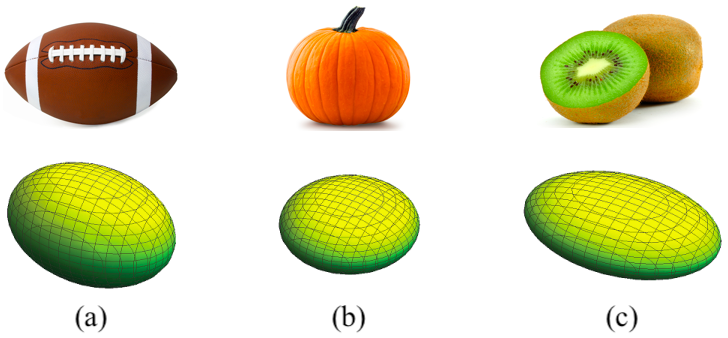
\includegraphics[width=0.8\textwidth]{Images/nuclear-shapes-v2.png}
	\caption{Nuclear shapes, adapted from \cite{MSU-shapes}. 
	\textbf{(a)} The shape of a elongated (prolate) derformed nucleus looks like an American football, while the shape of \textbf{(b)} a flattened (oblate) deformed nucleus looks like a pumpkin and \textbf{(c)} a triaxial deformed nucleus looks like a kiwi fruit.}
	\label{fig:Nuclear-shapes}
\end{figure}


\autoref{fig:cea_CoN} displays the chart of nuclides for deformed nuclei. 
The red lines in the figure corresponds to the magic numbers, i.e. the filling of shells. 
Around the red lines, the nuclei are marked with a gray color, meaning that there is no deformation. 
Between the red lines, where the shells are not filled, or half-filled, the nuclei are deformed and marked by a different color than gray. 

Nuclei in the rare-earth region, especially the samarium (Sm) isotopes, exhibits a variety of shape effects. 
\autoref{fig:Sm-shapes} shows that theory predicts that a transition from spherical to prolate shapes occurs within the Sm isotopes between $N = 82$ and $N = 94$.
The Sm isotope $^{144}_{~62}$Sm$_{82}$ has a closed neutron shell, and a spherical shape.
By adding neutrons to $^{144}$Sm, the deformation changes very rapidly to an prolate deformed shape at neutron number $N = 90$ ($^{152}$Sm). 
The transition from a spherical to a prolate deformed shape at $N = 90$ can be interpreted as a shape-phase transition, with the neutron number as control parameter. 
$^{152}$Sm happens to lie at the critical point of this phase transition \cite{Casten2001}.
Theory also predicts that an oblate deformed shape occur below the $N = 82$ shell closure, in $^{138}$Sm and $^{140}$Sm. 
Taking out more neutrons going to very neutron-deficient Sm nuclei, e.g. $^{132}$Sm, we also see a prolate deformed shape. 

Some nuclei exhibit what is called shape coexistence, i.e. the coexistence of quantum states that correspond to different shapes.
Shape coexistence is often found near closed shells and is possible for certain regions of $N$ and $Z$.
A typical indication for shape coexistence is $0^+$ states at low energy. 
One of the best examples for shape coexistence is the Hg (mercury) isotopes at neutron mid shell, around $^{186}_{~80}$Hg$_{106}$. 
The Hg isotopes are at $Z = 80$, just below the proton shell closure, $Z = 82$, and at neutron mid shell.
\textcolor{red}{Er det noen mer forklaring på hvorfor dette er det beste eksemplet? Påviste $0^+$ tilstander ved lav energi? Hvilke shapes ko-eksisterer? Artikkel?}

$^{140}_{~62}$Sm$_{78}$ is just below the neutron shell closure, $N = 82$, with a proton mid shell at $Z = 62$. 
In \Sm, there is an indication of two $0^+$ states around 1.6 MeV. 
One objective of this experiment is to clarify the structure of these $0^+$ states. 
The underlying nuclear structure is used as benchmarks for theoretical models.

An earlier experiment studying \Sm\ at CERN-ISOLDE found a triaxial shape for this isotope, i.e. a shape where all three principal axis of the ellipsoid have different lengths.
\Sm\ can therefore be considered to lie at the critical point of a phase-shape transition from spherical to deformed, and from prolate to oblate shape.
\textcolor{red}{Kan dette forklares uten å se på Potential Energy Surface (PES)? Denne figuren kommer egentlig senere, men bør kanskje flyttes?}
%\textcolor{blue}{In the previous experiment, there was an indication for triaxiality/\ga-softness \cite{Klintefjord} for \Sm, another form of shape-phase transition / critical point behavior, E(5) \cite{Iachello2000}. 
%\Sm\ could be one of the best examples of E(5) symmetry, need transition probabilities from higher-lying states to confirm.} \textcolor{red}{Denne må vel bort? Ellers er jeg ute å kjøre i teoriland...}
The previous experiment found an indication for \ga-softness (or potential triaxial shape). 
\Sm\ has therefore a transitional character between spherical and deformed shape, and at the same time in between prolate and oblate shape.
Theoretical models make predictions for nuclei with such symmetries \cite{Iachello2000}, and the present experiment are aiming to test these predictions.

Transition probabilities and quadrupole moments between several excited states in \Sm\ are still unknown.
With this experiment we want to measure $B(E2)$ values and quadrupole moments for higher-lying states.
Especially transitions from excited $0^+$ states will give information about possible shape coexistence or critical-point symmetry. 

\begin{figure}[htb]
	\centering
	\begin{subfigure}{\textwidth}
		\centering
		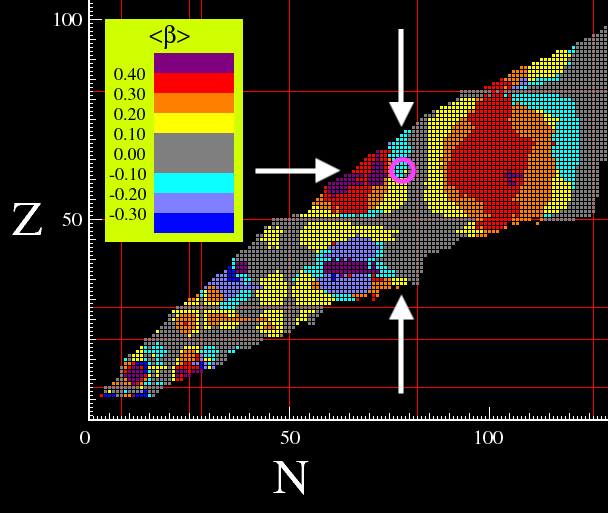
\includegraphics[width=0.9\textwidth]{Images/cea-CoN-adjusted.png}
		\caption{}
		\label{fig:cea_CoN}
	\end{subfigure}
	\begin{subfigure}{\textwidth}
		\centering
		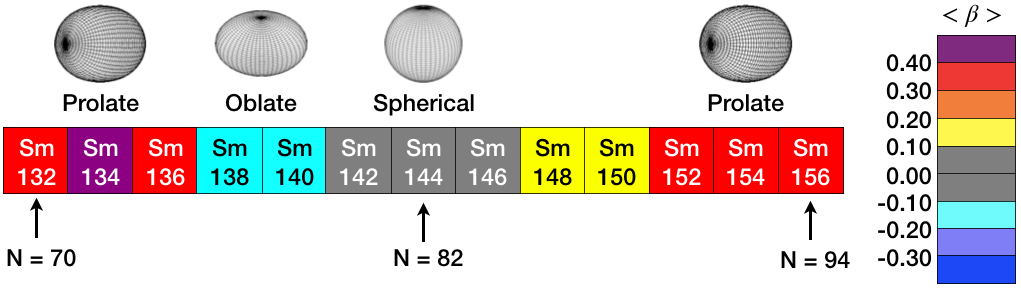
\includegraphics[width=\textwidth]{Images/Sm-shapes.png}
		\caption{}
		\label{fig:Sm-shapes}
	\end{subfigure}
	\caption{\textbf{(a)} Chart of nuclides for deformed nuclei, adapted from \cite{Hilaire2007, CEA}. \Sm\ is inside the pink ring, to the left of the yellow square.
	 \textbf{(b)} Sm shape transitions of even-even nuclei based on \cite{Hilaire2007, CEA}.
	 $\langle \beta \rangle > 0$ corresponds to a prolate shape, $\langle \beta \rangle = 0$ corresponds to a spherical shape and $\langle \beta \rangle < 0$ corresponds to an oblate shape.}
	\label{fig:deformation}
\end{figure}



\bigskip

A similar experiment, with experiment code IS495 titled \textit{Coulomb excitation of} \Sm, was conducted in 2012 at CERN-ISOLDE.
The old REX-ISOLDE post-accelerator was limited to a beam energy of 2.85 MeV/u for \Sm\ (samarium), which gave a low Coulomb excitation cross section and a low probability for multi-step excitations. 
At that time, a secondary target of $^{94}_{42}$Mo$_{52}$ (molybdenum) with a thickness of 2 mg/cm$^2$ was chosen to maximize the cross section at this energy.
From the excitation cross section it is possible to extract electromagnetic matrix elements, which are the observables that can be related to the nuclear shape.
Excited states up to 1256 keV were populated.
One goal of the experiment was to deduce the $B(E2)$ values and quadrupole moments of low-lying states in \Sm\ using multi-step Coulomb excitation.
A normalization of the $B(E2; 0^+ \rightarrow 2^+)$ value for \Sm\ to the well-known $B(E2)$ value for the Mo target, i.e. the transition strengths in the excited $^{94}$Mo target, was performed in order to extract the other $B(E2)$ values for \Sm.
It is necessary to know how many particles there are in the beam to determine a cross section.
This is difficult to measure.
Since the $B(E2)$ value of Mo was known, the excitation probability for Mo could be used to figure out how many particles there were in the beam, and hence get the excitation probabilities for Sm.
Out of the IS495 experiment (and another experiment) came a PhD thesis by Malin Klintefjord, titled \textit{Evolution of deformation and collectivity away from magic numbers} \cite{Klintefjord}, in addition to three articles \cite{Klintefjord2015, Samorajczyk2015, Klintefjord2016} on \Sm.

In the experiment in 2012, previously unknown transition strengths between low-lying states in \Sm\ was extracted. 
\ga\ intensities as a function of particle scattering angle was studied to get information about the first and second excited $2^+$ state, in addition to the first $4^+$ state.
\Sm\ was thought to have a low-lying $0^+$ state \cite{Firestone}, but this state was shown to be $2^+$ \cite{Samorajczyk2015}. 
The results of the experiment indicated a weak quadrupole deformation with a strong triaxiality or \ga-softness.

In 2017, there was an upgrade of the ISOLDE facility, which lead to the possibility of delivering beam energies up to 7.5 MeV/u. 
This allows for Coulomb excitation of \Sm\ at higher energies than the previous experiment.
In turn, this implied that it was possible to choose a high-$Z$ target (Pb) to give a high COULomb EXcitation (COULEX) cross section, especially for multi-step.
A beam energy of 4.65 MeV/u was chosen as the highest possible energy for safe COULEX for Pb.
COULEX will be discussed in \autoref{sec:Coulex}.
Excited states up to at least the $8^+$ state at 2970 keV are expected to be populated with this energy.
Maybe also currently unknown states will be populated.
This will give a greater understanding of the low-lying nuclear structure in \Sm.
With a new experiment, it will also be easier to interpret the nuclear shape of \Sm.

For the present experiment, no normalization of the transition probabilities were required.
From the previous experiment \cite{Klintefjord2016} and from lifetime measurements \cite{BelloGarrote2015}, the $B(E2, 0_1^+ \rightarrow 2_1^+$) value of \Sm\ was obtained. 
This can be used to normalize the transition probabilities for the higher-lying transitions.





\bigskip

\textcolor{red}{Si noe om appendix + GitHub?}

Beam energies are usually given in $\frac{\text{keV}}{\text{u}}$ or $\frac{\text{MeV}}{\text{u}}$.
This comes from 
\begin{align}
	\frac{\text{MeV}}{\text{A}} &= \frac{\text{MeV}}{\text{A}}  \frac{\text{A}}{\text{u}} = \frac{\text{MeV}}{\text{u}}  &  1 ~\text{A} &= 1 ~\text{u} \implies 1 = \frac{\text{A}}{\text{u}}
\end{align}
where $A$ is the mass number and $u$ is the atomic mass unit.

\bigskip

The goal of the master thesis is to analyze Coulomb excitation data of \Sm\ from an experiment at CERN-ISOLDE in 2017. The details of the experiment is outlined in \autoref{sec:exp_setup}. 

\bigskip

\textcolor{red}{A goal of the thesis is to document and make the procedure of the data analysis more transparent.}

% ----------------------------------------------------------------------------------------------------------------------
% ----------------------------------------------------------------------------------------------------------------------

\chapter{Theory}\label{ch:theory}
\epigraph{\textit{"I think I can safely say that nobody understands quantum mechanics."}}{\textit{– Richard Feynman}}


\section{Nuclear deformation}\label{sec:deformation}
%A way to understand nuclear deformation is to imagine a liquid drop vibrating \textcolor{red}{??? and/or rotating ???} at \textcolor{red}{??? high / a ???} frequency. 
%In this imagined picture, the average shape of the liquid drop nucleus is spherical, but the instantaneous shape is not.
It is natural to imagine nuclei as tiny spheres.
Although the nucleus is a fuzzy quantum object, we can still associate a macroscopic shape with it.
Thus we can define shape parameters that quantify the degree of deformation in the intrinsic system of the nucleus. 
These shapes can fluctuate (vibrations), and a deformed nucleus can also rotate in space.
The intrinsic shape does not change in case of rotation, but the description in the laboratory frame becomes time dependent. 
Although we can associate a deformation, it is not necessarily rigid. 
The moment of intertia is typically smaller than for a rigid system of the same deformation (think raw vs. boiled egg).

\autoref{fig:vibrating-nucleus} displays a sketch of a deformed vibrating nucleus.
One way to parameterize the instantaneous surface of the nucleus is to describe it by a vector \textbf{R} pointing from the origin to a surface point given by the angles $\theta$ and $\phi$ \cite{Krane}.
This is called the multipole expansion, and is given by the following equation
\begin{equation}\label{eq:Rfull}
	\mathbf{R}(\theta, \phi) = R_0 \left( 1 + a_{00} + \sum^\infty_{\lambda = 1} \sum^{+\lambda}_{\mu = -\lambda} a_{\lambda \mu} Y_{\lambda \mu}(\theta, \phi) \right)
\end{equation}
where $R_0$ is the radius of the sphere, $a_{00}$ describes volume changes, $a_{\lambda \mu}$ are the expansion coefficients, or the deformation parameters. 
The parametrization involves the spherical harmonics $Y_{\lambda \mu}$, where $\lambda$ is the multipole, $\mu$ is the order of the expansion and $\theta$ and $\phi$ are the intrinsic angles \cite{Krane, RS, Klintefjord}. 

\begin{figure}[ht]
	\centering
	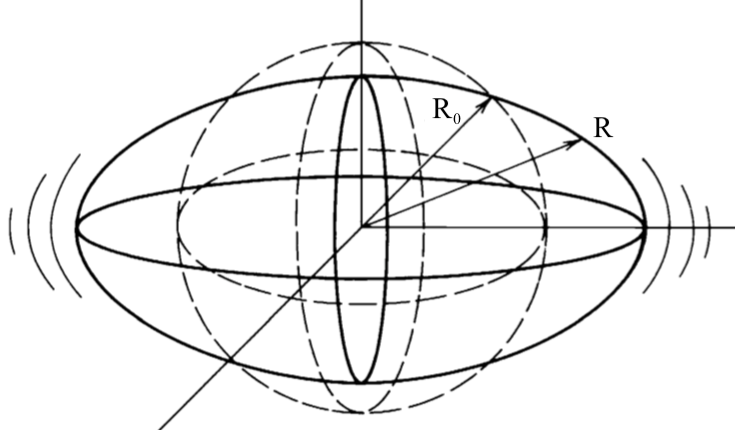
\includegraphics[width=0.6\textwidth]{Images/vibrating-nucleus.png}
	\caption{A deformed vibrating nucleus, adapted from \cite{Krane}. In the drawing, the dotted lines represent the spherical equilibrium shape. The drawing is an exaggerated to visualize the effect. See text for more information.}
	\label{fig:vibrating-nucleus}
\end{figure}

By assuming incompressibility of the nucleus, the volume is kept constant as
\begin{align*}
	V = \frac{4}{3} \pi R_0^3
\end{align*}
Further we have that
\begin{equation}\label{eq:radius}
	R_0 = r_0 A^{1/3}
\end{equation}
where $r_0 \approx 1.25$ fm and $A$ is the mass number of the nucleus.

The expansion coefficients, $a_{\lambda \mu}$, can be time dependent and can thus describe a vibration or rotation in space of the nucleus. 
%By reflection symmetry, the expansion coefficients are required to keep the equality $a_{\lambda \mu} = a_{\lambda, -\mu}$ \cite{Krane}.
Up to second order, the expansion coefficients are given as
\begin{equation}
	a_{00} = -\frac{1}{4\pi} \sum_{\lambda > 1, \mu} | a_{\lambda\mu} |^2
\end{equation}

\autoref{fig:vibrational-modes} shows a examples for changes in dipole, quadrupole and octupole parameters.
The dipole term, $\lambda = 1$, describes a translation of the whole system, and this is not very interesting in it self. 
Translational motion describes the motion of a system. 
Higher-order deformations play a role only in a few selected regions of the nuclear chart, and a large majority of nuclei can be described by quadrupole ($\lambda = 2$) shapes.
By putting the origin of the coordinate system in the center of mass, it is possible to fix and exclude the $a_{1\mu}$ parameters, and thus also $a_{00}$ \cite{RS}. 
If we restrict the system to small deformations, we get that $a_{1\mu} = 0$ and thus $a_{00} = 0$.
\autoref{eq:Rfull} is then reduced to
\begin{equation}\label{eq:Rmid}
	\mathbf{R}(\theta, \phi) = R_0 \left( 1 +  \sum^\infty_{\lambda = 2} \sum^{+\lambda}_{\mu = -\lambda} a_{\lambda \mu} Y_{\lambda \mu}(\theta, \phi) \right)
\end{equation}

Another condition is that $\mathbf{R}$ should be invariant under reflection and rotation of the coordinate system, i.e. $R$ should be unchanged by transformations of the coordinate system.
%By further choosing the $z$-axis as symmetry axis, we end up in a special case where all $a_{\lambda \mu}$ vanishes except when $\mu = 0$. 
%This is the assumption of axial symmetry.
%The special parameters, $a_{\lambda 0}$, are called $\beta_2$.

The quadrupole deformation, $\lambda = 2$, is the most important mode.
It describes the shape of the nucleus and is the dominant feature in most of the deformed nuclei. 
In nuclei with spherical shape, the quadrupole vibrations are the lowest mode of collective excitations.
Deformed nuclei, on the other hand, have low-lying rotational states.
%With low multipolarity, the quadrupole vibration is the first available vibrational mode for low-energy excitation in nuclei.
In almost all even-even nuclei there is a low-lying state with $J^\pi = 2^+$, and near closed shells it is possible to distinguish the second harmonic states as well ($J^\pi = 0^+, 2^+, 4^+$). 
A quadrupole vibration has spin 2 and is connected via an electric quadrupole transition to the ground state. 
For a two-phonon excitation, two quadrupole excitation couples, each of which has spin 2.
If you have two spin vectors, they can couple to spin 0, 2 and 4, they cannot couple to odd spins if there is axial symmetry.
\textcolor{red}{Skal jeg forklare phonon?}

\begin{figure}[ht]
	\centering
	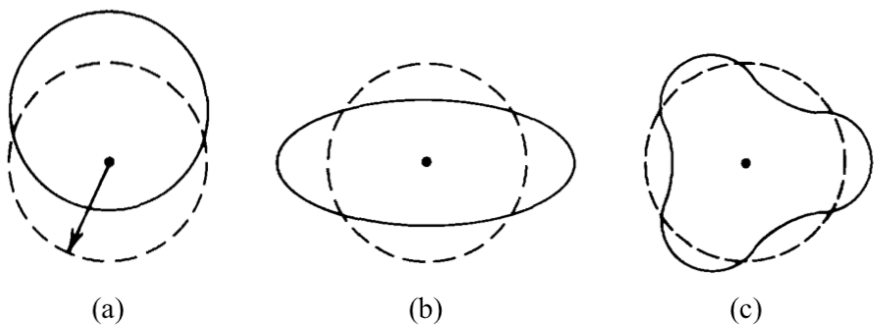
\includegraphics[width=0.8\textwidth]{Images/vibration-modes-3.png}
	\caption{Vibrational modes, adapted from \cite{Krane}. The dotted lines represent the spherical equilibrium shape.
	(a) Dipole, $\lambda = 1$. 
	(b) Quadrupole, $\lambda = 2$. 
	(c) Octupole, $\lambda = 3$.}
	\label{fig:vibrational-modes}
\end{figure}
%(d) Hexadecapole, $\lambda = 4$, $a_{40} > 0$. \cite{RS}
%(e) Hexadecapole, $\lambda = 4$, $a_{40} < 0$.

For $\lambda = 2$, there are five parameters of $a_{2\mu}$ ($\mu \in \{ -2, -1, 0, 1, 2 \}$). 
Two parameters describe the shape, and in addition there are three parameters describing the orientation in space. %(Euler angles $\Omega = (\alpha, \beta, \gamma)$). 
It is possible to align the deformed shape in a coordinate system such that only two parameters are needed to describe the shape of the nucleus.
With a suitable rotation, we can achieve 
\begin{align*}
	a_{21} &=  a_{2,-1} = 0 \\
	a_{22} &= a_{2,-2} 
\end{align*}
leaving two independent parameters, $a_{20}$ and $a_{22}$. 
With Hill-Wheeler \cite{Hill-Wheeler} coordinates ($\beta$, $\gamma$) they become
\begin{align}
	a_{20} &= \beta \cos \gamma \label{eq:a-param1} \\
	a_{22} &= \frac{1}{\sqrt{2}} \beta \sin \gamma \label{eq:a-param2}
\end{align}
where $\beta$ is axial deformation (deformation magnitude) and $\gamma$ is triaxial deformation (shape parameter). 
$\gamma = 0$ and $\beta > 0$ corresponds to  the prolate deformed shape, while $\gamma = 0$ and $\beta < 0$ corresponds to the oblate shape. 
The triaxial shape is obtained when $0 < \gamma < \tfrac{\pi}{3}$.
Further we have
\begin{equation}
	\sum_\mu | a_{2\mu} |^2 = a_{20}^2 + 2a_{22}^2 = \beta^2
\end{equation}
In the special case when $\lambda = 2$, \autoref{eq:Rmid} becomes
\begin{equation}
	\mathbf{R}(\theta, \phi) = R_0 \left( 1 + \beta \sqrt{\frac{5}{16\pi}} (\cos \gamma (3\cos^2 \theta - 1) + \sqrt{3} \sin \gamma \sin^2 \theta \cos 2\phi) \right)
\end{equation}
by using the spherical harmonics $Y_{20}$ and $Y_{2,\pm 2}$ \cite{RS}.

The equilibrium shape of a nucleus can be characterized by a potential energy surface (PES) in the $\beta$-\ga\ plane if we restrict the deformation to quadrupole shapes. 
\autoref{fig:collective_modes} displays sketches of three extreme cases of potential energy surfaces; spherical vibrator, deformed rotor and \ga-soft rotor.
The steeper a minimum in the PES, the more rigid is the deformation. 
Accordingly, a more shallow potential means that the shape is softer against vibrations. 
Two competing shapes, i.e. shape coexistence, would show up as two minima in the PES. 
\autoref{fig:cea_tri} shows the PES of \Sm.
It is essentially flat in both $\beta$ and \ga\ direction. 
That is consistent with our earlier interpretation of \Sm\ as a transition nucleus in between spherical and deformed and in between prolate and oblate shape. 
In principle, the potential can be reasonably well approximated by a square well potential, in which case the Schrödinger equation can be solved analytically. 
%This is exactly what the E(5) model does.

\begin{figure}[htb]
	\centering
	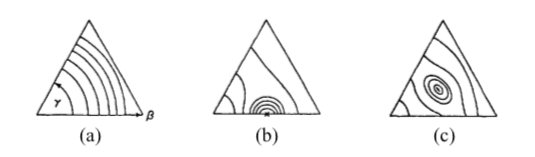
\includegraphics[width=0.9\textwidth]{Images/collective_modes.png}
	\caption{Potential energy surface, adapted from \cite{Heyde}.
	\textbf{(a)} Spherical vibrator.
	\textbf{(b)} Deformed rotor. %, $\beta = 0.5\beta_0$ and $\gamma = 0^\circ$.	
	\textbf{(c)} \ga-soft rotor.
	See the text for more information.
	}
	\label{fig:collective_modes}
\end{figure}

\begin{figure}[htb]
	\centering
	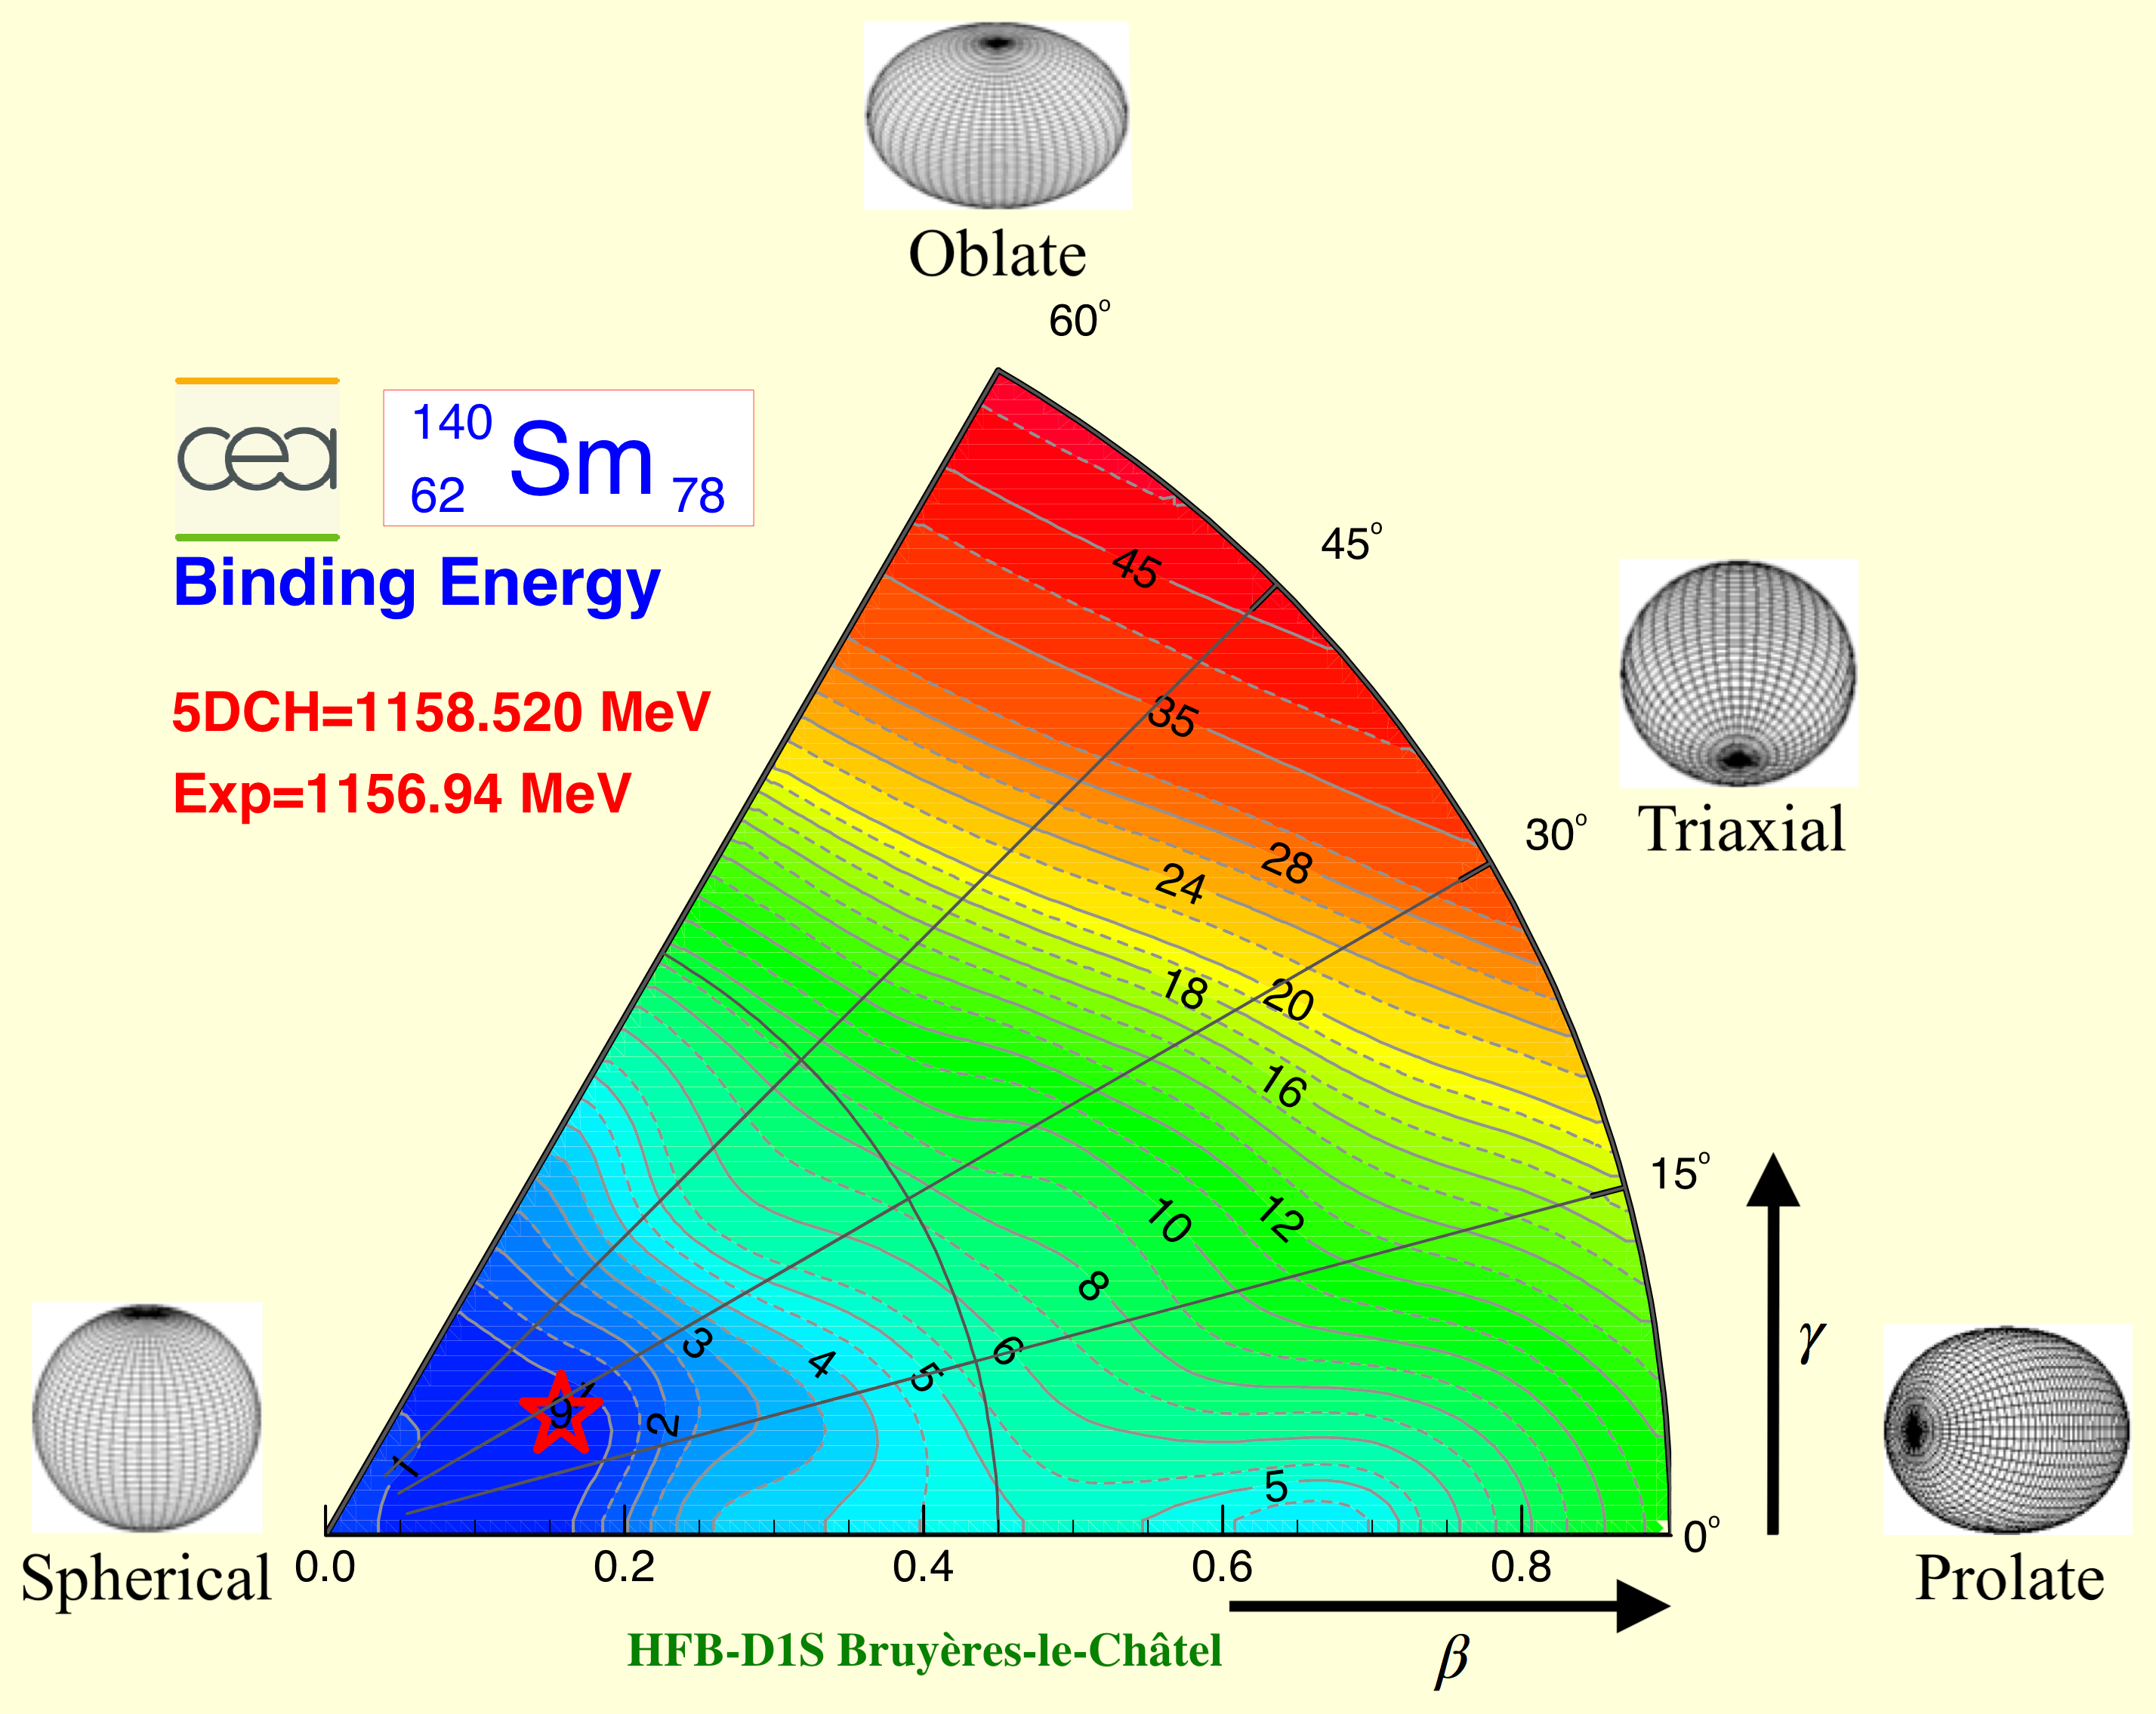
\includegraphics[width=0.7\textwidth]{Images/Triaxial-map-drawing.png}
	\caption{Potential energy surface for \Sm, adapted from \cite{Hilaire2007, CEA}. 
	See the text for more information.}
	\label{fig:cea_tri}
\end{figure}

Octupole vibration, $\lambda = 3$, with $J^\pi = 3^-$ can be seen in many nuclei in certain regions of the nuclear chart, where orbitals with a spin difference of 3 are available near the Fermi surface.
In nuclei where the shell structure makes the quadrupole modes occur at very high energies, such as in doubly magic nuclei, the octupole state is often the lowest excited state.
The octupole deformation has a pear shape.


\section{The Coulomb excitation method}\label{sec:Coulex}
COULomb EXcitation (COULEX) is an experimental method to excite a nucleus by an inelastic scattering with another nucleus through the electromagnetic interaction. 
%The elastic Coulomb scattering process is also known as Rutherford scattering.
%Inelastic Coulomb scattering is called Coulomb excitation.
This method is very useful for studying collective excitations and shapes of nuclei, as they are often connected by electric quadrupole transitions.  
Transition energies and intensities can be used to determine new excited levels and study deformation.
An extensive description of Coulomb excitation can be found in \cite{Alder1956, EE-Coulex, Bertulani2009}.

\autoref{fig:scattering} shows sketches of the scattering process in the LABoratory (LAB) and Center of Mass (CM) frame of reference. 
In the LAB frame, a beam particle approaches the target with a velocity $\mathbf{u}$ in a straight line in the absence of the repulsive force. 
The beam particle gets excited by the electromagnetic interaction with the target particle. 
It is of course also possible that the target nucleus gets excited, or that there is no excitation, i.e. elastic scattering. 
It is even possible, although not very likely, that both target an projectile get excited simultaneously.
We are only considering the case where the projectile gets excited.
This excitation is an unstable energy state and rapidly thereafter it will de-excite, sending out a \ga-ray.
Both the beam and target particles are scattered with a velocity $\mathbf{v}_b$ and $\mathbf{v}_t$ respectively.
The distance, $b$, is called the impact parameter and is the vertical distance between the beam and target particle. 
$V_{cm}$ is the center of mass velocity. 
The angles $\theta_b$ and $\theta_t$ are the scattering angles for the beam and target particle, respectively. 
A small angle $\theta_b$ means forward scattering of the beam, a larger distance between the beam particle and the target particle, a weaker electromagnetic (EM) field and less excitation probability. 
A large angle $\theta_b$ means backward scattering of the beam, a closer distance between the beam particle and the target particle, a stronger EM field and higher excitation probability.
In the CM frame, the center of mass velocity is zero, and the velocities and angles are marked by an apostrophe to separate between the two frames of reference.

The Coulomb scattering kinematics can be approximated by an elastic collision.
In \autoref{ch:scattering}, a calculation of the two-particle elastic collision is performed.

\begin{figure}[htb]
	\centering
	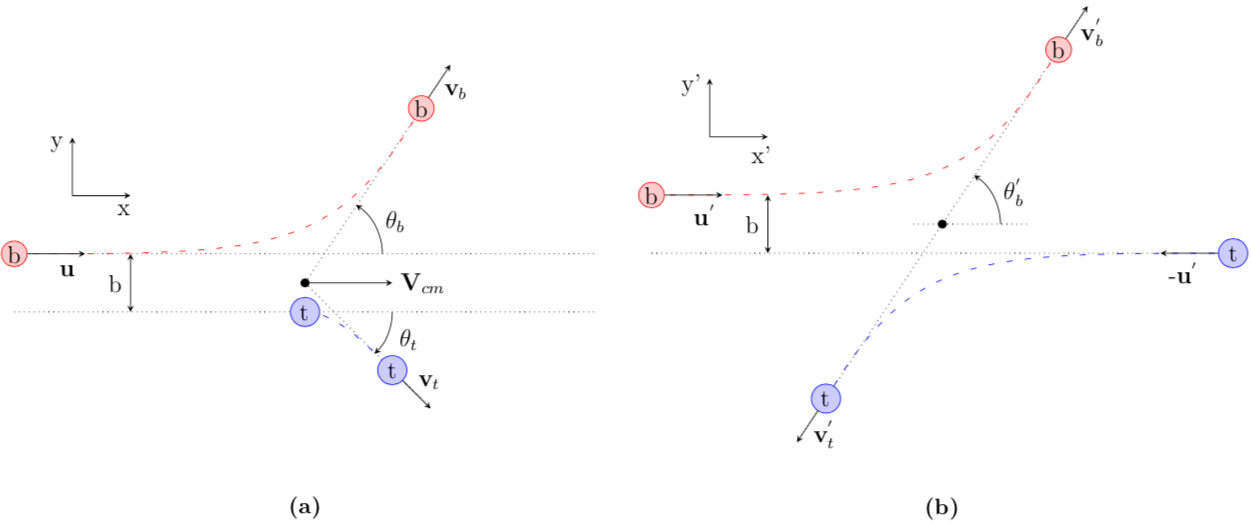
\includegraphics[width=\textwidth]{Images/scattering.png}
	\caption{Scattering in different frames of reference.
	\textbf{(a)} Scattering in the LABoratory (LAB) frame. 
	\textbf{(b)} Scattering in the Center of Mass (CM) frame. 
	See text for more information.}
	\label{fig:scattering}
\end{figure}

%\begin{figure}[ht]
%	\centering
%	\begin{subfigure}{\textwidth}
%		%%
%% Laboratory frame
%%
\begin{tikzpicture}
    % Definitions
    \coordinate (Bleft)  at (-5,0.5);
    \coordinate (Bright) at (5,0.5);
    \coordinate (origo)  at (0,0);
    \coordinate (Tleft)  at (-5,-0.5);
    \coordinate (Tright) at (5,-0.5);
    \coordinate (Bup)    at (2,3);
    \coordinate (Tstart) at (0,-0.5);
    \coordinate (Tdown)  at (1.5,-1.5);
    % Lines
    \draw[dotted] (Tleft) -- (Tright);
    \draw[dotted] (Bleft) -- (Bright);
    \draw[dotted] (origo) -- (Bup);   % particle angle line
    \draw[dotted] (origo) -- (2,-2);  % target angle line
    % Particle paths
    \draw[red,loosely dashed]  (Bleft)  .. controls (-0.5,0.5) and (0.5,0.5) .. (Bup);
    \draw[blue,loosely dashed] (Tstart) .. controls (0.5,-0.5) and (1,-1)    .. (Tdown);
    % Impact parameter
    \draw[<->, >=stealth] (-3,0.5) -- node[left] {b} (-3,-0.5);
    % Center of mass
    \draw[fill=black] (origo) circle[radius=0.07cm] node {};
    \draw[->, >=stealth] (origo) -- (1.5,0) node[right] {$\textbf{V}_{cm}$}; % CM help line
    % Angles
    \draw[->, >=stealth] (1.33,0.5) arc (0:57:1cm)  node[right,pos=0.6,outer sep=1mm] {$\theta_b$};
    \draw[->, >=stealth] (1.5,-0.5) arc (0:-46:1cm) node[right,pos=0.6,outer sep=1mm] {$\theta_t$};
    % Vectors
    \draw[->, >=stealth] (-4.78,0.5) -- ++(1,0)        node[below,pos=0.7,outer sep=0.5mm] {$\textbf{u}$};
    \draw[->, >=stealth] (Bup)       -- ++(0.5,0.75)   node[right,pos=0.4,outer sep=0.6mm] {$\textbf{v}_b$};
    \draw[->, >=stealth] (Tdown)     -- ++(0.66,-0.66) node[right,pos=0.3,outer sep=1.2mm] {$\textbf{v}_t$};
    % Particles
    \draw[draw=blue,fill=blue!20] (Tdown)  circle[radius=0.25cm] node {t};
    \draw[draw=blue,fill=blue!20] (Tstart) circle[radius=0.25cm] node {t};
    \draw[draw=red,fill=red!20]   (Bleft)  circle[radius=0.22cm] node {b};
    \draw[draw=red,fill=red!20]   (Bup)    circle[radius=0.22cm] node {b};
    % Coordinate system 
    \coordinate (CSP) at (-4,1.5);
    \draw[->, >=stealth] (CSP) -- ++(1,0) node[below, pos=0.9] {x};
    \draw[->, >=stealth] (CSP) -- ++(0,1) node[left, pos=0.9]  {y};
    % Vertical alignment with CM frame
    \node[] at (-7.08,0) {};
    % Vertical space from caption text
    \node[] at (0,-2.5) {};
\end{tikzpicture}
%		\caption{}
%		\label{fig:LAB}
%	\end{subfigure}
%	\begin{subfigure}{\textwidth}
%		%%
%% Center of mass frame
%%
\begin{center}
\begin{tikzpicture}
    % Definitions
    \coordinate (Bleft)  at (-5,0.5);
    \coordinate (Bright) at (5,0.5);
    \coordinate (origo)  at (0,0);
    \coordinate (Tleft)  at (-5,-0.5);
    \coordinate (Tright) at (5,-0.5);
    \coordinate (Bup)    at (2,3);
    \coordinate (Tdown)  at (-2,-3);
    % Lines
    \draw[dotted] (Tleft)  -- (3.75,-0.5);
    \draw[dotted] (Tdown)  -- (Bup);    % 180 degree line
    \draw[dotted] (-0.5,0) -- (1.5,0);  % angle help line
    % Particle paths
    \draw[red,loosely dashed]  (Bleft)  .. controls (-0.5,0.5) and (0.5,0.5)   .. (Bup);
    \draw[blue,loosely dashed] (Tright) .. controls (0.5,-0.5) and (-0.5,-0.5) .. (Tdown);
    % Impact parameter
    \draw[<->, >=stealth] (-3,0.5) -- node[left] {b} (-3,-0.5);
    % Center of mass
    \draw[fill=black] (origo) circle[radius=0.07cm] node {};
    % Angles
    \draw[->, >=stealth] (1,0) arc (0:57:1cm) node[right, pos=0.6, outer sep=1mm] {$\theta_b^{'}$};
    % Vectors
    \draw[->, >=stealth] (-4.78,0.5) -- ++(1,0)        node[below, pos=0.7] {$\textbf{u}^{'}$};
    \draw[->, >=stealth] (4.75,-0.5) -- ++(-1,0)       node[below, pos=0.6] {-$\textbf{u}^{'}$};
    \draw[->, >=stealth] (Bup)       -- ++(0.5,0.75)   node[right, pos=0.4,outer sep=0.5mm] {$\textbf{v}_b^{'}$};
    \draw[->, >=stealth] (Tdown)     -- ++(-0.5,-0.75) node[right, pos=0.8,outer sep=0.5mm] {$\textbf{v}_t^{'}$};
    % Particles
    \draw[draw=blue,fill=blue!20] (Tdown)  circle[radius=0.25cm] node {t};
    \draw[draw=blue,fill=blue!20] (Tright) circle[radius=0.25cm] node {t};
    \draw[draw=red,fill=red!20]   (Bleft)  circle[radius=0.22cm] node {b};
    \draw[draw=red,fill=red!20]   (Bup)    circle[radius=0.22cm] node {b};
    % Coordinate system 
    \coordinate (CSP) at (-4,1.5);
    \draw[->, >=stealth] (CSP) -- ++(1,0) node[below, pos=0.9] {x'};
    \draw[->, >=stealth] (CSP) -- ++(0,1) node[left, pos=0.9] {y'};
    % Vertical space from LAB frame
    \node[] at (0,4.5) {};
\end{tikzpicture}
\end{center}
%		\caption{}
%		\label{fig:CM}
%	\end{subfigure}
%	\caption{Scattering in different frames of reference.
%	(a) Scattering in the LABoratory (LAB) frame. A small angle $\theta_b$ means forward scattering of the beam, a larger distance between the beam particle and the target particle, a weaker electromagnetic (EM) field and less excitation probability. A large angle $\theta_b$ means backward scattering of the beam, a closer distance between the beam particle and the target particle, a stronger EM field and a higher excitation probability.
%	(b) Scattering in the Center of Mass (CM) frame.}
%	\label{fig:LAB-CM}
%\end{figure}



\textcolor{red}{Burde jeg brukt projectile and target under her?}

In the semi-classical approach of Coulomb excitation theory, the projectile (beam) and target is assumed to move on hyperbolic paths. 
This approach does not take into account the energy loss during the excitation process.
When the beam particle approaches the target particle, the beam particle reaches a minimum separation distance, $d$, which is dependent on the impact parameter $b$. 
The distance of closest approach, $d$, is the distance between the center of both nuclei. 
In a head-on collision, $b = 0$ and the particles reach the distance of closest approach $d$, which is given by
\begin{equation}
	d\left( \theta_b^{'} \right) = a \left( 1 + \csc \left( \frac{\theta_b^{'}}{2} \right) \right) = a \left( 1 + \frac{1}{\sin \left( \frac{\theta_b^{'}}{2} \right)} \right) ~[\text{fm}]
\end{equation}
The scattering angle of the beam in the CM frame is $\theta_b^{'}$.
Half the distance of closest approach, $a$, in a head-on collision ($\theta_b^{'} = 180^\circ$) is given by
\begin{equation}
	 a = \tfrac{1}{2} d = \frac{Z_b Z_t e^2}{m_r v_i^2} ~[\text{fm}]
\end{equation}
$Z_b$ and $Z_t$ is the proton number of the beam and target, respectively. 
The elementary charge is $e$, the initial velocity of the beam is $v_i$ and $m_r$ is the reduced mass of the beam and target given by
\begin{align}
	 m_r &= m_b \frac{A_b A_t}{A_b + A_t} = m_b A_r  ~\left[ \tfrac{\text{MeV}}{\text{c}^2} \right]
	 &
	 A_r &= \frac{A_b A_t}{A_b + A_t}
\end{align}
where $m_b$ is the mass of the beam particle, and $A_r$ is the reduced mass number of the beam and target \cite{RBass, EE-Coulex}. 
The impact parameter can be expressed as
\begin{equation}
	b = a \cot \left( \tfrac{\theta_b^{'}}{2} \right)
\end{equation}

One requirement in the semi-classical approach is that the asymptotic wavelength of relative motion of the beam, i.e. the de Broglie wavelength ${\lambdabar = \hbar/m_r v_i}$, must be small compared to the distance of closest approach, $d$ \cite{RBass, EE-Coulex}.
The ratio of half the distance of closest approach and the de Broglie wavelength defines the Sommerfeld parameter, $\eta$, which measures the strength of the Coulomb interaction \cite{Cline1969}.
It is given by
\begin{equation}
	\eta = \frac{d}{2\lambdabar} = \frac{a}{\lambdabar} = \frac{Z_b Z_t e^2}{m_r v_i^2} = \frac{Z_b Z_t e^2}{\hbar v_i} \approx 0.72 \frac{Z_b Z_t}{A_r E_b}
\end{equation}
where $E_b = \tfrac{1}{2} m_b v_i^2$ is the initial kinetic energy of the beam given in MeV/u \cite{RBass}.
A requirement for describing the relative motion of the particles in the CM frame by hyperbolic paths is that $\eta \gg 1$.
%In the case of Coulomb excitation with heavy ions, the semi-classical approach and assumption of classical trajectories are justified.
%In the semi-classical approach, this is fairly accurate \cite{Cline1969}. 
The factor 0.72 comes from 
\begin{align}
	\frac{e^2}{2} = \frac{(\sqrt{1.4399764 ~[\text{MeV} \cdot \text{fm}]})^2}{2} \approx 0.72 ~[\text{MeV} \cdot \text{fm}]
\end{align}

Another important parameter is the adiabaticity parameter, $\xi$, which is given by 
\begin{equation}
	\xi = \frac{\tau_c}{\tau_{ex}} = \frac{a}{\hbar v_i}  \Delta E = \frac{Z_b Z_t e^2}{\hbar v_i} \cdot \frac{\Delta E}{2E_b} = \eta \cdot \frac{\Delta E}{2E_b}
\end{equation}
where $\tau_c = \frac{a}{v_i}$ is the collision time and $\tau_{ex} = \frac{\hbar}{\Delta E}$ is the excitation time.
The probability of exciting the nucleus from a initial state $|i\rangle$ to a final state $|f\rangle$ with excitation energy difference $\Delta E = E_f - E_i$ is dependent on the adiabaticity parameter \cite{Niedermaier, NaR, RBass}.
If $\xi \ll 1$ the reaction process is sudden and the excitation probability is largest, while if $\xi \gg 1$ the reaction becomes adiabatic, which means that the reaction process becomes hindered. 
The excitation probability decreases exponentially with increasing $\xi$. 
A semi-classical approach of the Coulomb excitation is a good approximation if the conditions $\eta \gg 1$ and $\xi \ll 1$ are fulfilled.
This means that the energy transfer has negligible influence of the motion and thus  
\begin{equation}
	\frac{\Delta E}{E_b} \ll 1
\end{equation}
which will not hold for all states $|f\rangle$.
The conditions are fulfilled for states with a considerable excitation probability \cite{EE-Coulex, RBass}.


\subsection{Safe COULEX}
In order to ensure that the interaction is purely electromagnetic in nature, and not nuclear, a safe energy is chosen for the reaction. 
The energy is supposed to be below the Coulomb barrier.
Safe COULEX is when the distance of closest approach between the particles is large enough to exclude nuclear interaction.
The safety distance, $d_{safe}$, in safe COULEX is chosen by the condition
\begin{align}
	d_{safe} \geq d_{min} &= d_C + d_s \nonumber \\
	&= R_b + R_t + d_s \nonumber \\
	&= r_0 (A_b^{1/3} + A_t^{1/3}) + d_s \nonumber \\
	&= 1.25 (A_b^{1/3} + A_t^{1/3}) + 5~\text{[fm]}
\end{align}
where $d_{min}$ is a way to approximate the distance of closest approach by the Coulomb interaction distance, $d_C$, and an additional safety distance, $d_s = 5$ fm.
$R_b$ and $R_t$ is the radii of the beam and target nuclei, respectively, and $A_b$ and $A_t$ is the mass number of the beam and target nuclei, respectively \cite{RBass, Cline1986}.

The maximum beam energy in the LAB frame, $E_{b, max}$, is chosen from the special case when $\theta_b^{'} = 180^\circ$ \cite{Klintefjord, RBass}
\begin{align}
	E_{b, max} (\theta_b^{'})
	&= \frac{Z_b Z_t e^2}{A_r d_{min}} \cdot \frac{2}{1 + \csc \left( \frac{\theta_b^{'}}{2} \right)} \\
	&\approx \frac{Z_b Z_t}{A_r} \cdot \frac{1.44}{1.25 (A_b^{1/3} + A_t^{1/3}) + 5} ~\left[ \tfrac{\text{MeV}}{\text{u}} \right]
\end{align}

%For \Sm\ on \Pb\ the safe beam energy is 4.63 MeV/u. 
%The experiment was run with a beam energy of 4.65 MeV/u, so it is really at the limit of what can be considered safe for head-on collisions.
%The maximum CM angle covered with the setup is $136^\circ$, so for the angular range that is covered by the experiment, the beam energy is safe.

For the reaction, only the energy, $E^{'}$, and relative momentum in the CM frame is available, while the remainder is recoil energy, $E_t$, of the total system
\begin{equation}
	E_t = \frac{A_b}{A_b + A_t} E_b
\end{equation}
In the CM frame, the kinetic energy is given by
\begin{equation}
	E^{'} = E_b - E_t = \frac{A_t}{A_b + A_t} E_{b}
\end{equation}
where $A_b$ and $A_t$ is the mass number of the beam and target nuclei and $E_{b}$ is the kinetic energy of the beam particle in the LAB frame \cite{Niedermaier, NaR}.


\subsection{Cross sections}
For point-like charges, the differential scattering cross section, $d\sigma_R$, is given by the the classical Rutherford formula
\begin{align}
	\frac{d\sigma_R}{d\Omega} 
	&= \frac{a^2}{4 \sin \left( \tfrac{\theta_b^{'}}{2} \right)} \nonumber \\
	&= \left( \frac{Z_b Z_t e^2}{4\pi \varepsilon_0}  \right)^2 \left( \frac{1}{4 E_b}  \right)^2 \cdot \frac{1}{\sin^4 \left( \frac{\theta_b^{'}}{2} \right)} \nonumber \\	
	&= \left( \frac{Z_b Z_t e^2}{8 \pi \varepsilon_0 m_b v_0^{' 2}} \right)^2 \cdot \frac{1}{\sin^4 \left( \frac{\theta_b^{'}}{2} \right)} 
\end{align}
where $d\Omega$ is the solid angle, $Z_b$ and $Z_t$ is the proton number of the beam and target nuclei respectively, $e$ is the elementary charge, $\varepsilon_0$ is the electric permittivity in vacuum, $m_b$ is the mass of the beam particle, $v_i^{'}$ is the initial velocity of the beam particle in the CM frame and $\theta_b^{'}$ is the beam particle scattering angle in the CM frame \cite{Klintefjord, Krane, EE-Coulex}.

Under the condition, $\xi \ll 1$, the differential cross section, $d\sigma_{i \rightarrow f}$, for inelastic scattering of point-like objects from the initial state $|i\rangle$ to the final state $|f\rangle$ is given by 
\begin{align}
	\frac{d\sigma_{i \rightarrow f}}{d\Omega} 
	&= \frac{d\sigma_R}{d\Omega} \cdot P_{i \rightarrow f} 
\end{align}
The excitation probability, $P_{i \rightarrow f}$, is given by
\begin{equation}
	P_{i \rightarrow f} = \frac{1}{2I_i + 1} \sum_{M_i, M_f} | a_{if} |^2
\end{equation}
where $I_i$ is the spin of the state $|i\rangle$, $M_i$ and $M_f$ is the angular momentum projections of initial and final states, respectively \cite{EE-Coulex, NaR}.
$a_{if}$ is the excitation amplitudes summed over all magnetic substates, which can be expressed by
\begin{equation}
	a_{if} = \frac{1}{i\hbar} \int_{-\infty}^{\infty} e^{i \frac{\Delta E}{\hbar} t} \langle f | H(t) | i \rangle ~dt
\end{equation}
where $\Delta E = E_f - E_i$ is the energy difference of the final and initial state, respectively, $H(t)$ is the time-dependent electromagnetic interaction between the beam and the target \cite{Klintefjord, Niedermaier, NaR}.

The total electric excitation cross section from a state $|i\rangle$ to a state $|f\rangle$ is given by
\begin{equation}\label{tot_sig_E}
	\sigma_E = \sum_\lambda \sigma_{E \lambda}
\end{equation}
with
\begin{equation}\label{sig_E}
	\sigma_{E \lambda} = \left( \frac{Z_b e}{\hbar v_i} \right)^2 a^{-2 \lambda + 2} B(E \lambda; I_i \rightarrow I_f) f_{E \lambda} (\xi)
\end{equation}
The reduced transition probability, $B(E \lambda)$, is related to the matrix elements of the electric multipole order by
\begin{equation}
	B(E \lambda; I_i \rightarrow I_f) = \frac{1}{2I_i + 1} | \langle f | \mathcal{M}(E \lambda)| i \rangle |^2 
\end{equation}
and the Coulomb excitation function, $f_{E \lambda} (\xi)$ is given by
\begin{equation}
	f_{E \lambda} (\xi) = \int_\Omega df_{E \lambda} (\theta_b^{'}, \xi)
\end{equation}
where the integration is performed over all scattering angles of the solid angle $\Omega$ in the CM frame \cite{Niedermaier, EE-Coulex}.
The Coulomb excitation function is dependent on $\xi$ and the multipolarity. 
In a special case with $E2$ transitions and $\xi \ll 1$, the function is $f_{E \lambda} (\xi) \approx 1$.
From the reduced transition probabilities with $\lambda = 2$, it is possible to show that \autoref{sig_E} becomes \cite{NaR}
\begin{equation}
	\sigma_{E2} \approx \left( \frac{Z_b e}{\hbar v_i} \right)^2 a^{-2} = \left( \frac{mv_i}{Z_t e\hbar} \right)^2
\end{equation}

Similarly to the total electric cross section, the total magnetic cross section can be expressed as \cite{EE-Coulex}
\begin{equation}
	\sigma_M = \sum_\lambda \sigma_{M \lambda} = \left( \frac{Z_b e}{\hbar c} \right)^2 \sum_\lambda a^{-2 \lambda + 2} B(M \lambda; I_i \rightarrow I_f) f_{M \lambda} (\xi)
\end{equation}
The equations are very similar, but notice the $1/c$ in the first fraction, in addition to the switching of $E$ to $M$.
This means that magnetic excitations are suppressed by a factor $(v/c)^2$, which means that magnetic excitations do not play any role in practice.
The excitation process is purely electric, but the decay of the excited states can be both electric and magnetic.


\subsection{Transition probabilities}

The transition probability of going from a state $|i\rangle$ to a state $|f\rangle$ is
\begin{align}
	T_{i \rightarrow f} (\sigma \lambda) = \frac{8\pi (\lambda + 1)}{\lambda \hbar [(2\lambda + 1)!!]^2} \left( \frac{E_\gamma}{\hbar c} \right)^{2\lambda + 1} B(\sigma \lambda; I_i \rightarrow I_f)
\end{align}
where $\sigma \lambda$ is the multipolarity with $\sigma \in \{ E, M \}$. 
Transition with the lowest multipolarity, i.e. small $\lambda$, are most likely, while transitions of high multipolarity are relatively unlikely. 
Electric transitions are more probable than magnetic transitions of the same multipolarity.
%A gamma quant of multipolarity $\lambda$ carries angular momentum $\lambda \hbar$ with $z$ component $\mu \hbar$.
The reduced transition probability is
\begin{align}
	B(\sigma \lambda; I_i \rightarrow I_f) &= \sum_{M_i, M_f} | \langle I_f M_f | \hat{O}_{\lambda \mu} | I_i M_i \rangle |^2  \nonumber \\
	&= \frac{1}{2I_i + 1} | \langle I_f | \hat{O}_{\lambda \mu} | I_i \rangle |^2
\end{align}
 and $\hat{O}_{\lambda \mu} \in \{ \hat{E}_{\lambda \mu}, \hat{M}_{\lambda \mu} \}$ is the electric or magnetic multipole operator.
By measuring transition probabilities it is possible to measure $B(E2)$ values (and other multipolarities), and these quantities are closely related to the nuclear shape and can be compared to theoretical calculations.

The reduced transition probabilities are not the same if the spin states are interchanged
\begin{align}
	B(\sigma \lambda; I_f \rightarrow I_i) &\neq B(\sigma \lambda; I_i \rightarrow I_f)
\end{align}
while an interchange of the reduced matrix elements does not matter
\begin{align}
	| \langle I_f | \hat{O}_{\lambda \mu} | I_i \rangle |^2 &= | \langle I_i | \hat{O}_{\lambda \mu} | I_f \rangle |^2
\end{align}
There is a relation of the reduced transition probability between the excitation $B(E2 \uparrow)$ and the decay $B(E2 \downarrow)$ of a state, which is given by 
\begin{equation}
	B(E2; I_f \rightarrow I_i) = \frac{2I_i + 1}{2I_f + 1} B(E2; I_i \rightarrow I_f)
\end{equation}
For an $E2$ transition from the ground state $0_1^+$ and the first excited state $2_1^+$, we have the relation
\begin{align}
	B(E2; 0_1^+ \rightarrow 2_1^+) = 5 \cdot B(E2; 2_1^+ \rightarrow 0_1^+)
\end{align} 
This means that the excitation probability has five times more final substates to go to, compared to the decay probability as displayed by \autoref{fig:transitions}.

\begin{figure}[htb!]
	\centering
	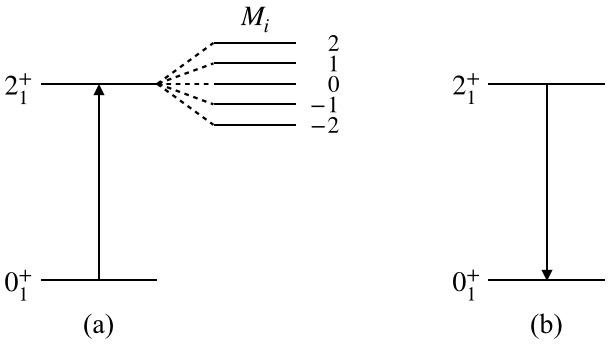
\includegraphics[width=0.6\textwidth]{Images/transitions.png}
	\caption{\textbf{(a)} Excitation probability. \textbf{(b)} Decay probability.}
	\label{fig:transitions}
\end{figure}


\autoref{tab:gamma_sel} shows the \ga\ selection rules where the parity \cite{Krane} is decided by
\begin{align}
	\pi (\sigma \lambda) =
    \begin{cases}
    		(-1)^\lambda, & \text{for } \sigma \lambda = E\lambda \\
    		(-1)^{\lambda + 1}, & \text{for } \sigma \lambda = M\lambda
    \end{cases}
\end{align}
and angular momentum conservation gives
\begin{align}
 	| I_i - I_f | \leq \lambda \leq I_i + I_f 
\end{align}

\begin{table}[htb!] 
    \centering 
    \caption{\ga\ selection rules. Electric transitions are more likely than magnetic transitions of the same multipole $\lambda$. There are no \ga\ transitions with $\lambda = 0$, i.e. no $I_i = 0 \rightarrow I_f = 0$. The $0 \rightarrow 0$ transitions proceed via internal conversion or internal pair creation.}
	% Data for the Gamma selection rules table
\begin{tabular}{cccccc}
\hline
$|\Delta I|$       & 0    &  1   &  2   &  3   & 4    \\
\hline
$\Delta \pi =$ yes &  E1  &  E1  &  M2  &  E3  &  M4  \\
                   & (M2) & (M2) &  E3  & (M4) &  E5  \\
\hline
$\Delta \pi =$ no  &  M1  &  M1  &  E2  &  M3  &  E4  \\
                   &  E2  &  E2  & (M3) &  E4  & (M5) \\
\hline
\end{tabular}
	\label{tab:gamma_sel}
\end{table}




\subsection{Electric quadrupole moments}

The electric quadrupole moment is a parameter that describes the charge distribution of a nucleus and thus its shape.
In the classical definition it is given by
\begin{align}
	Q_{ij} = \int \rho(\mathbf{r}) (3r_i r_j - r^2 \delta_{ij}) ~d^3 \mathbf{r}
\end{align}
where $\rho$ is the charge density distribution, $\mathbf{r} = (r_1, r_2, r_3) = (x, y, z)$ are the Cartesian coordinates, $i,j \in \{ 1, 2, 3 \}$ and
\begin{align}
	\delta_{ij} =
    \begin{cases}
    		0, & \text{if } i \neq j \\
    		1, & \text{if } i = j
    \end{cases}
\end{align}
is the Kronecker delta.
It is possible to rotate the frame such that the $z$-axis coincides with the symmetry axis. 
With axial symmetry \cite{Niedermaier, ELP}, we choose the $z$-axis along the symmetry axis and gets
\begin{align}
	Q_z &= \int \rho(\mathbf{r}) (3z^2 - r^2) ~d \mathbf{r} \nonumber \\
	&=  \int \rho(\mathbf{r}) (3\cos^2 \theta - 1) ~d \mathbf{r} \nonumber \\
	&=  \sqrt{\frac{16\pi}{5}} \int \rho(\mathbf{r}) r^2 Y_{20}(\theta, \phi) ~d \mathbf{r} \nonumber \\
	&= Q_{20}
\end{align}
In this case, the charge distribution is fully characterized by $Q_z$, because symmetry gives $Q_x = Q_y$. 
$Q_z = 0$ corresponds to a spherical shape, while $Q_z > 0$ corresponds to a prolate shape and $Q_z < 0$ corresponds to a oblate shape.
In the same way as $Q_{20}$, it is possible to define 
\begin{align}
	Q_{22} &= \sqrt{\frac{16\pi}{5}} \int \rho(\mathbf{r}) r^2 Y_{22}(\theta, \phi) ~d \mathbf{r}
\end{align}
All quadrupole shapes can be described by $Q_{20}$ and $Q_{22}$ in a similar way as all quadrupole shapes can be described by $\beta$ and \ga. These are the definitions of the quadrupole moment in the intrinsic frame of the nucleus.

For a state with spin $I$ we can observe the spectroscopic quadrupole moment
\begin{align}
	Q_s(I) &= \langle I, m = I | \hat{Q}_{20} | I, m = I \rangle \\
	&= \sqrt{\frac{I(2I - 1)}{(2I + 1)(2I + 3)(I + 1)}} \langle I | \hat{Q}_2 | I \rangle
\end{align}
where $\hat{Q}_2$ is the electric multipole operator \cite{RS} from
\begin{align}
	\hat{Q}_{\lambda \mu} = \int \rho(\mathbf{r}) r^\lambda Y_{\lambda \mu}(\theta, \phi) ~d^3 \mathbf{r}
\end{align}
The spectroscopic quadrupole moment is what we can observe in the LAB frame.
Here we see that $I = 0$ or $\tfrac{1}{2}$ gives $Q_s = 0$, which means that a nucleus with these spins can have intrinsic deformation, but it cannot be measured via the spectroscopic quadrupole moment \cite{ELP}.  

The intrinsic quadrupole moment, $Q_0$, is in the body-fixed frame.
It is related to the spectroscopic quadrupole moment via
\begin{align}
	Q_s = \frac{3K^2 - I(I+1)}{(I+1)(2I+3)} Q_0
\end{align}
where $K$ is the projection of total angular momentum onto the body-fixed symmetry axis.
$K$ is only defined if there is a symmetry axis, i.e. if the nucleus has rotational symmetry.
If the total angular momentum is perpendicular to the symmetry axis, then $K = 0$.
The intrinsic quadrupole moment, $Q_0$, reflects the nuclear deformation, $\beta$, and is related via \cite{Klintefjord, LOBNER1970}
\begin{align}
	Q_0 &= \int \rho(\mathbf{r}) (3z^2 - r^2) ~d \mathbf{r} \nonumber \\
	&\approx \frac{3}{\sqrt{5\pi}} Z R^2 (\beta + 0.16 \beta^2)
\end{align}
If the intrinsic shape is prolate, $Q_0 > 0$, the measurements shows an oblate shape in the laboratory frame, $Q_s < 0$.
A prolate deformed nucleus that is rotating rapidly about the perpendicular axis appears to be oblate.
Obtaining information on $Q_s$ and the relative signs of matrix elements can help us to directly distinguish between prolate and oblate shape.


% ----------------------------------------------------------------------------------------------------------------------
% ----------------------------------------------------------------------------------------------------------------------

\chapter{Coulomb excitation experiment}
\epigraph{\textit{"If I could remember the names of all those particles, I'd be a botanist."}}{\textit{– Enrico Fermi}}

\section{ISOLDE at CERN}
ISOLDE is a Radioactive Ion Beam (RIB) facility at CERN in Meyrin, Switzerland. \autoref{fig:accelerators} shows the CERN accelerator complex, where ISOLDE is located beside the Proton Synchrotron Booster (PSB), in the lower right marked by a green box. The acronym ISOLDE stands for Isotope Separator On Line DEvice. The facility can produce over 1000 different radionuclides to be used in a wide variety of experiments in nuclear physics, atomic physics, solid state physics, life sciences and fundamental interactions. Experiments have been performed at ISOLDE since 1967 and since 2001 experiments with post-accelerated RIBs have been conducted  \cite{HIE-ISOLDE, ISOLDE-web, ISOLDE-facility}. 
The High Intensity and Energy upgrade (HIE-ISOLDE) made it possible to deliver beam energies up to 7.5 MeV/u in July 2017 \cite{CERN-news}. 
The present experiment was one of the first Miniball experiments with the upgraded superconducting LINear ACcelerator (LINAC), the HIE-ISOLDE LINAC. 
Further upgrades, after the present experiment, have made it possible to deliver beam energies up to 10 MeV/$u$ in 2018 \cite{HIE-ISOLDE}. 

\begin{figure}[ht]
	\centering
	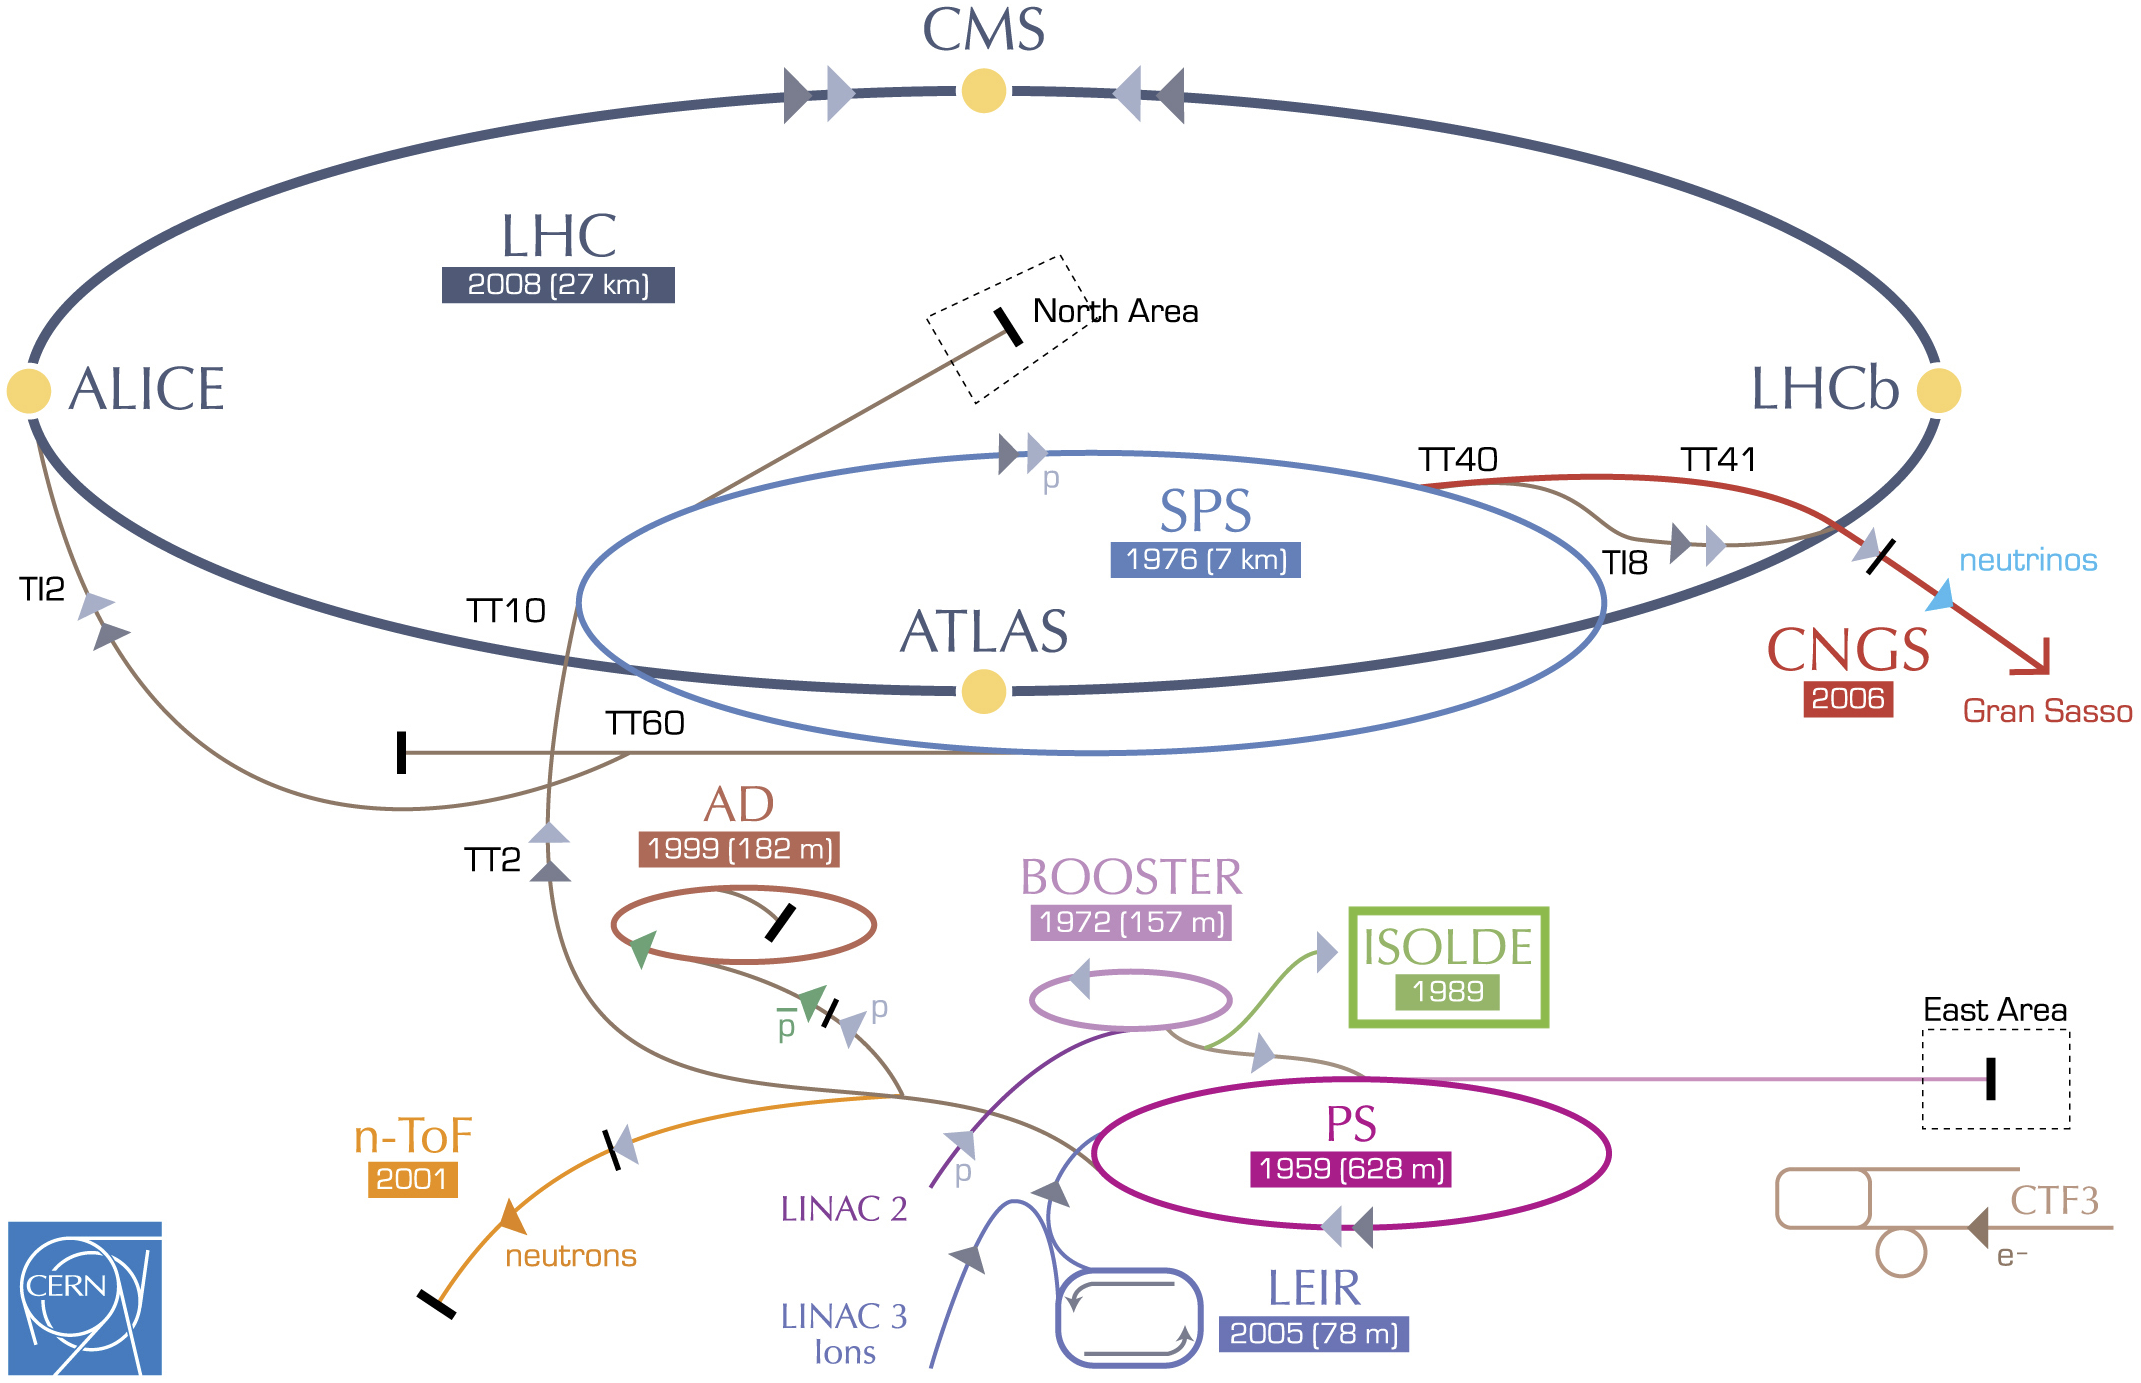
\includegraphics[width=\textwidth]{Images/CERN-accelerators.png}
	\caption{The CERN accelerator complex, adapted from \cite{CERN-AC}. ISOLDE, marked with a green box, receives accelerated protons from LINAC 2 and the PS Booster.}
	\label{fig:accelerators}
\end{figure}

In general, it is very challenging to study radioactive, short lived nuclei. 
The newest edition of the Karlsruhe Nuclide Chart have nuclear data of over 4000 nuclides, and most of these are radioactive \cite{CoN}. 
In many cases it is not possible produce a target of a radioactive nuclei and to perform experiments due to the short half-life of the involved nucleus. 
To study these radioactive nuclei, RIBs are accelerated at stable targets. 

The beam at the RIB facilities consists of, as the name implies, radioactive isotopes. 
In contrast to conventional facilities where the target is made out of the isotope of interest, the investigated isotope is the beam accelerated into a target.
The velocity of the beam is significant, with $v/c$ values of a few percent. 

One way of obtaining a RIB is to use the Isotope Separator On Line (ISOL) method. 
There are three main reactions for producing radioactive atoms with the ISOL method; spallation, fragmentation and fission. 
Nuclear spallation is the process in which light fragments of the target are ejected due to the high-energy impact of the incoming beam. 
Fragmentation is the splitting of a target compound into smaller particles or unstable ions. 
In fission, a nucleus is split into two or more nuclei.
When applying the ISOL method, two accelerator systems are required. 
The first accelerator is used to produce the radioactive atoms by spallation, fragmentation or fission of the primary target nuclei. 
Then, the second accelerator is used to accelerate the RIB atoms into a secondary target \cite{ISOLDE-web, Lindroos, ISOL}. 

In RIB facilities, the intensity is generally a bit lower compared to stable beam facilities, which is a big challenge. 
In terms of energy, ISOL facilities operate around the Coulomb barrier, making them suitable for Coulomb excitation and particle transfer reactions. 

In the electromagnetic (EM) interaction with the target, the beam gets excited into a higher energy state.
When the beam isotopes de-excite, they emit \ga-rays, which can be observed to have large Doppler shifts depending on the velocity and angle.
Due to the finite solid angle of the detectors, a sizable Doppler broadening can be observed in the \ga-rays. 
When the detection system has high granularity, i.e. that the system consists of many segmented detectors, the Doppler shifts and broadening can be corrected for. 
If the angle between the recoiling nucleus and the \ga-ray can be determined accurately, a Doppler correction can be applied \cite{MB-spect}, as described in \autoref{ssec:Doppler}.


\section{Experimental setup}\label{sec:exp_setup}

The Coulomb excitation experiment was a beam of \Sm\ accelerated into a target of \Pb\ at  an energy 4.65 MeV/u.
It was conducted between 8th and 14th of August in 2017 at the ISOLDE facility.
The experiment code was IS558 with the title \textit{Shape Transition and Coexistence in Neutron-Deficient Rare Earth Isotopes}.
\Sm\ is a radioactive isotope with a ground state half-life ($T_{1/2}$) of 14.82 min, and is a neutron-deficient nuclei compared to the line of stability.

%Samarium (Sm) comes from the lanthanide series of chemical elements, which are known as rare-earth elements.
%\Sm\ is a radioactive isotope with a ground state half-life ($T_{1/2}$) of 14.82 min, and is a neutron-deficient nuclei compared to the line of stability.

\begin{itemize}
	\item \textcolor{red}{Forskningsgrupper som samarbeidet om eksperimentet?}
	\item \textcolor{red}{Nevne/minne leser på hva som er målet med eksperimentet og grovt hvordan det gjøres?}
\end{itemize}


\subsection{Beam production}\label{ssec:beam_prod}
\autoref{fig:Coulex} shows a sketch of the experimental setup of the \Sm\ Coulomb excitation experiment. 
Accelerated proton beam bunches from the PSB comes into the ISOLDE facility and collide with a thick production target, the primary target. 
Two proton beam bunches are separated by 1.2 s.
The proton beam has an energy of 1.4 GeV and an intensity up to 2 $\mu$A \cite{TIF, TIF2013}. 
ISOLDE typically takes 50\% \cite{MB-spect} of all proton bunches form the PSB, the rest goes to the Large Hadron Collider (LHC) and the other experiments shown in \autoref{fig:accelerators}. 

\begin{figure}[ht]
	\centering
	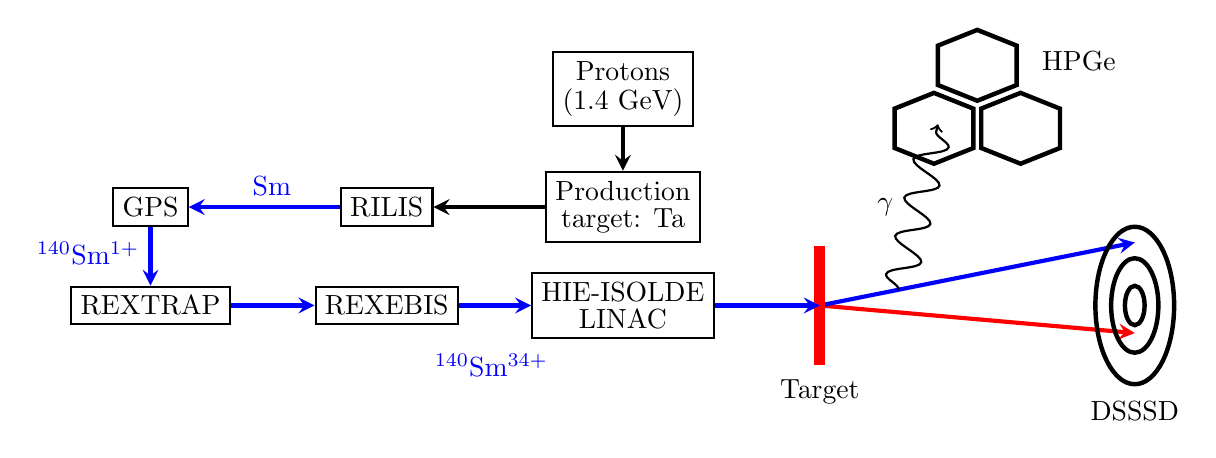
\begin{tikzpicture}
    % Definitions
    \coordinate (origo)   at (0,0);
    \coordinate (Protons) at (-2.5,2.75);
    \coordinate (GPS)     at (-8.5,1.25);
    \coordinate (RILIS)   at (-5.5,1.25);
    \coordinate (PTarget) at (-2.5,1.25);
    \coordinate (REXTRAP) at (-8.5,0);
    \coordinate (REXEBIS) at (-5.5,0);
    \coordinate (HILinac) at (-2.5,0);
    % Target and lines from target
    \draw[->,red,>=stealth,line width=1.5pt] (origo) -- (4,-0.35);
    \draw[->,blue,>=stealth,line width=1.5pt] (origo) -- (4,0.8);
    \draw[red, line width=4pt] (0,0.75) -- (0,-0.75) node[black, below] {Target};
    % Nodes
    \node(P)   at (Protons) [draw,thick] {\shortstack{Protons \\ (1.4 GeV)}};
    \node(G)   at (GPS)     [draw,thick] {GPS};
    \node(R)   at (RILIS)   [draw,thick] {RILIS};
    \node(PT)  at (PTarget) [draw,thick] {\shortstack{Production \\ target: Ta}};
    \node(RXT) at (REXTRAP) [draw,thick] {REXTRAP};
    \node(RXE) at (REXEBIS) [draw,thick] {REXEBIS};
    \node(LIN) at (HILinac) [draw,thick] {\shortstack{HIE-ISOLDE \\ LINAC}};
    % Arrows
    \draw[->,>=stealth,line width=1.5pt]      (P) -- (PT);
    \draw[->,>=stealth,line width=1.5pt]      (PT) -- (R);
    \draw[->,blue,>=stealth,line width=1.5pt] (R) -- (G) node[anchor=south, pos=0.45] {Sm};
    \draw[->,blue,>=stealth,line width=1.5pt] (G) -- (RXT) node[anchor=east, pos=0.45] {$^{140}$Sm$^{1+}$};
    \draw[->,blue,>=stealth,line width=1.5pt] (RXT) -- (RXE);
    \draw[->,blue,>=stealth,line width=1.5pt] (RXE) -- (LIN) node[anchor=north, pos=0.45, outer sep=5mm] {$^{140}$Sm$^{34+}$};
    \draw[->,blue,>=stealth,line width=1.5pt] (LIN) -- (origo);
    % CD 
    \draw[ultra thick] (4,0) ellipse [x radius=0.25cm,y radius=0.125cm, rotate=90];
    \draw[ultra thick] (4,0) ellipse [x radius=0.6cm,y radius=0.3cm, rotate=90];
    \draw[ultra thick] (4,0) ellipse [x radius=1cm,y radius=0.5cm, rotate=90] node[anchor=north, outer sep=11mm] {DSSSD};
    % HPGe
    %\draw (2,2.5) circle (1cm);
    \draw[ultra thick]  (0.95,2) -- ++(0.5,-0.2) -- ++(0.5,0.2) -- ++(0,0.5) -- ++(-0.5,0.2) -- ++(-0.5,-0.2) -- cycle;
    \draw[ultra thick] (1.5,2.8) -- ++(0.5,-0.2) -- ++(0.5,0.2) -- ++(0,0.5) -- ++(-0.5,0.2) -- ++(-0.5,-0.2) -- cycle;
    \draw[ultra thick]  (2.05,2) -- ++(0.5,-0.2) -- ++(0.5,0.2) -- ++(0,0.5) -- ++(-0.5,0.2) -- ++(-0.5,-0.2) -- cycle;
    \node[anchor=west] at (2.7,3.1) {HPGe};
    % Gamma
    \draw[->, decoration={snake,segment length=5mm,amplitude=2mm},decorate,thick] (1,0.2) -- (1.5,2.3) node[left, pos=0.5, outer sep=2mm] {$\gamma$};
\end{tikzpicture}
	\caption{The Coulomb excitation setup at ISOLDE for the present experiment. Adapted from \cite{Klintefjord}. See text for information.}
	\label{fig:Coulex}
\end{figure}

The production target material is chosen depending on the RIB of interest. 
If the requested RIB is neutron-rich, a primary target of uranium ($^{238}$U) is chosen, and the beam will be produced by fission of the target nuclei.
In this experiment, a neutron-deficient RIB was requested, and a primary target of tantalum (Ta, $Z = 73$) was chosen.
The production target is selected from a region in the chart of nuclides containing stable nuclei that are heavier than the nucleus of interest.
When the proton beam collides with the primary target, the target is smashed into pieces, and radioactive isotopes with proton number up to Ta are produced.
In this way, a large range of isotopes are produced. 

The remaining challenge is to extract the isotope of interest in order to create a RIB. 
Before the desired isotope can be obtained, a method of selecting the chemical element of interest have to be used.
One approach is to use a method of selective ionization and then a high voltage electrostatic field to extract the ions. 
Electronic transitions are characteristic for each chemical element. 
A laser with a precisely tuned wavelength can obtain the photon energy that matches the electronic transition energies in the atom perfectly \cite{RILIS-web, RILIS2013}. 
Thus we can use one laser to excite an electron to a specific excited electron-state in the atom, a second laser to excite electrons further to another excited electron-sate and a third laser to remove the electron entirely. 
In this way, we only ionize the element required to produce the beam. 

The Resonance Ionization Laser Ion Source (RILIS) is based on the method of step-wise (2-3 step) excitation and ionization of an atom. 
It is an element-selective process which is used to produce ion beams of the desired element \cite{RILIS}. 
In this experiment, RILIS was used to select samarium (Sm) with atomic number $Z = 62$. 
After RILIS has selected Sm, we have a continuous beam of Sm$^{+1}$ ions at an energy of 60 keV. 
\textcolor{blue}{The primary target is on a 60 kV high voltage platform} \textcolor{red}{??? fjerne eller utdype ???} \cite{ISOLDE-web, TIF}. 

After the ionization of the beam, the next step in the process is to perform a mass separation.
The goal of the mass separation is to obtain a beam only containing the isotopes with the desired mass number, and to exclude the contaminants that exits RILIS. 
By using a set of magnets, the separator purifies the RIB, but in principle, isobaric contaminants may still be present in the beam after the separation. 
Luckily, the neighboring elements of Sm produces very little surface ionization. 
Therefore, few contaminants are expected to be present in the beam after the separator. 
Different sources of beam contaminants are discussed in \autoref{ssec:bcontaminants}.

At ISOLDE, the beam may hit one of two target stations after RILIS; either the General Purpose Separator (GPS) or the High Resolution Separator (HRS). 
Both separators feed the beam lines in the experimental hall, but only one separator is active during an experiment. 
The HRS combine two bending magnets with high mass resolving power, delivering the beam into the main beam line. 
Even though the HRS have a high mass resolving power, $M/\Delta M > 5000$, it is not sufficient resolving power to separate the isobars, which is why RILIS and the GPS was used in the current experiment.
The GPS has one bending magnet and can deliver beams containing isotopes of different mass numbers simultaneously into three beam lines. 
The two extra beam lines that the GPS can feed, can have an isotope mass difference of $\pm 13 \%$ compared to the main beam line isotope mass \cite{GPS, TIF}.
In this experiment the GPS was used to select the isotope of Sm with mass number $A = 140$. 

Following the GPS, a continuous beam of \Sm\ is obtained. 
The post-accelerator cannot accept an incoming continuous beam, it can only accelerate bunches.
In the Radioactive beam EXperiment TRAP (REXTRAP), the \Sm\ ions are collected in order to release them in bunches that are matched to the time structure of the HIE-ISOLDE LINAC. 
REXTRAP is a penning trap which tasks are accumulation, bunching and cooling of the RIB \cite{HIE-ISOLDE, REXTRAP1, REXTRAP2}. 
The ions are released in bunches and transfered to the REX Electron Beam Ion Source (REXEBIS), see \autoref{fig:Coulex}.

REXEBIS is a charge breeder where the RIB obtains a high charge state \cite{REXEBIS}, with a mass-to-charge ($A/q$) ratio typically between 2.5 and 4.5 \cite{Post-acc}.
In REXEBIS, even more electrons of the RIB atoms are removed through the interaction with a high-intensity electron beam. 
The longer the ions stay in REXEBIS, the higher the charge state becomes. 
The EBIS blasts off more electrons from Sm, which leaves the nucleus in a high charge state, going from \Sm$^{+1}$ to \Sm$^{+34}$ with $A/q \approx 4.1$. 

To accelerate the charged ions, i.e. the beam, to high energy, the beam must consist of highly charged ions. 
Inside REXEBIS a distribution of charge states are obtained, but the HIE-ISOLDE LINAC can only accept one charge state.
Therefore, only the parts of the RIB containing the correct charge state is accelerated, the remainder of the beam is lost \cite{REX-web, HIE-web, EBIS2002, EBIS2010}.
REXEBIS releases the beam with a specific energy through another mass separator before guiding the RIB into the HIE-ISOLDE LINAC. 
The purpose of the second mass separator is to remove residual gas (beam contaminants) from the beam exiting REXEBIS \cite{HIE-ISOLDE}. 

The HIE-ISOLDE LINAC accelerates the beam of \Sm\ with excellent purity to 4.65 MeV/u, or a total energy of 651 MeV, through the beam line. 
Several magnets bend the beam into the Miniball spectrometer, where the beam hits the secondary target of \Pb. 
The beam particles get excited due to the electromagnetic interaction with the target.
%There is a very small probability of exciting the target, explained in \autoref{ssec:Pb}.
As the \Sm\ particles from the beam fly towards the particle detector, they de-excite by emitting \ga-rays, which are then detected by the \ga\ detectors.
The detector system records information about the angles and energy with a good time resolution. 
In this way, particle-\ga\ coincidences can be reconstructed to obtain Doppler-corrected \ga-spectra  in order to analyze the Coulomb excitation of \Sm.


\subsection{Sources of beam contaminants}\label{ssec:bcontaminants}
To have a successful experiment, the purity of the beam is of great importance. Contaminants in the beam can come from several different sources. 
A common experimental challenge are contaminants from surface ionization, i.e. atoms that collide with the walls of the ion source. 
This can be significant, even dominant in some cases. 
However, surface ionization was not an issue in the present experiment due to the fact that Sm has the lowest ionization potential of the rare earth elements. 
In any case, the beam contaminants are monitored by periodically switching the laser on and off.
Arising from the primary target we may have \cite{MB-spect}:
\begin{itemize}
	\item isobaric contaminants which are inseparable by the mass separator because of the same mass number
	\item isotopes with an integer multiple of both mass and charge
\end{itemize}
and from stable isotopes the contaminants can come from:
\begin{itemize}
	\item buffer gas in REXTRAP (e.g. Ne, Ar)
	\item residual gas in REXEBIS (e.g. C, O)
	\item components of REXEBIS (e.g. La from the cathode)
\end{itemize}
More information on contaminants can be found in \cite{HIE-ISOLDE, RILIS, MB-spect}.

%\textcolor{Magenta}{Tilbakemelding: \newline
%Blir litt lange setninger for en liste øverst. Skriv om til tekst eller del opp i flere setninger. \newline
%"with an integer multiple of both mass an charge" er litt uforklarlig? \newline
%}

\subsection{The secondary target}\label{ssec:Pb}
For the current experiment, a target consisting of \Pb\ with a thickness of 1.4 mg/cm$^2$ was chosen. 
Unfortunately, there was a finger print on the target, implying a contamination (probably carbon and/or oxygen from grease).

It is quite difficult to excite $^{208}_{~82}$Pb$_{126}$ as it is a doubly magic nuclei, and it is therefore well suited for the experiment. 
In that way, transitions from the target will not complicate the \ga-ray spectrum.
With a target consisting of the highest possible $Z$ of a stable isotope ($Z = 82$), the excitation probability of \Sm\ is maximized. 

\Pb\ has no quadrupole deformation.
The first excited state is an octupole vibration with an energy of 2615 keV, a half-life of $T_{1/2} = 16.7$ ps and a spin and parity of $J^\pi = 3^-$.
Therefore, there is a small probability of observing the first excited state of \Pb\ in the \ga-spectrum. 
The excitation probability for \Pb\ is maximal if the EM interaction is approximately head on, and the ejected target nucleus hits one of the inner particle detector rings.


\subsection{Miniball spectrometer}
\autoref{fig:MBSpect} shows an overview picture of the Miniball spectrometer. 

\textcolor{Magenta}{Tilbakemelding:\newline
Legg til en intro setning, overfladisk beskriv hvordan Miniball ser ut og i grove trekk hvilke deler den består av.
}
\textcolor{red}{Skal jeg ha bilder av Miniball spektrometeret, eller skal jeg fjerne dem? Det er jo ikke akkurat som man ser så veldig masse.. evt. flytte til appendix? (skal i alle fall beholde target wheel)}

\begin{figure}[ht]
	\centering
	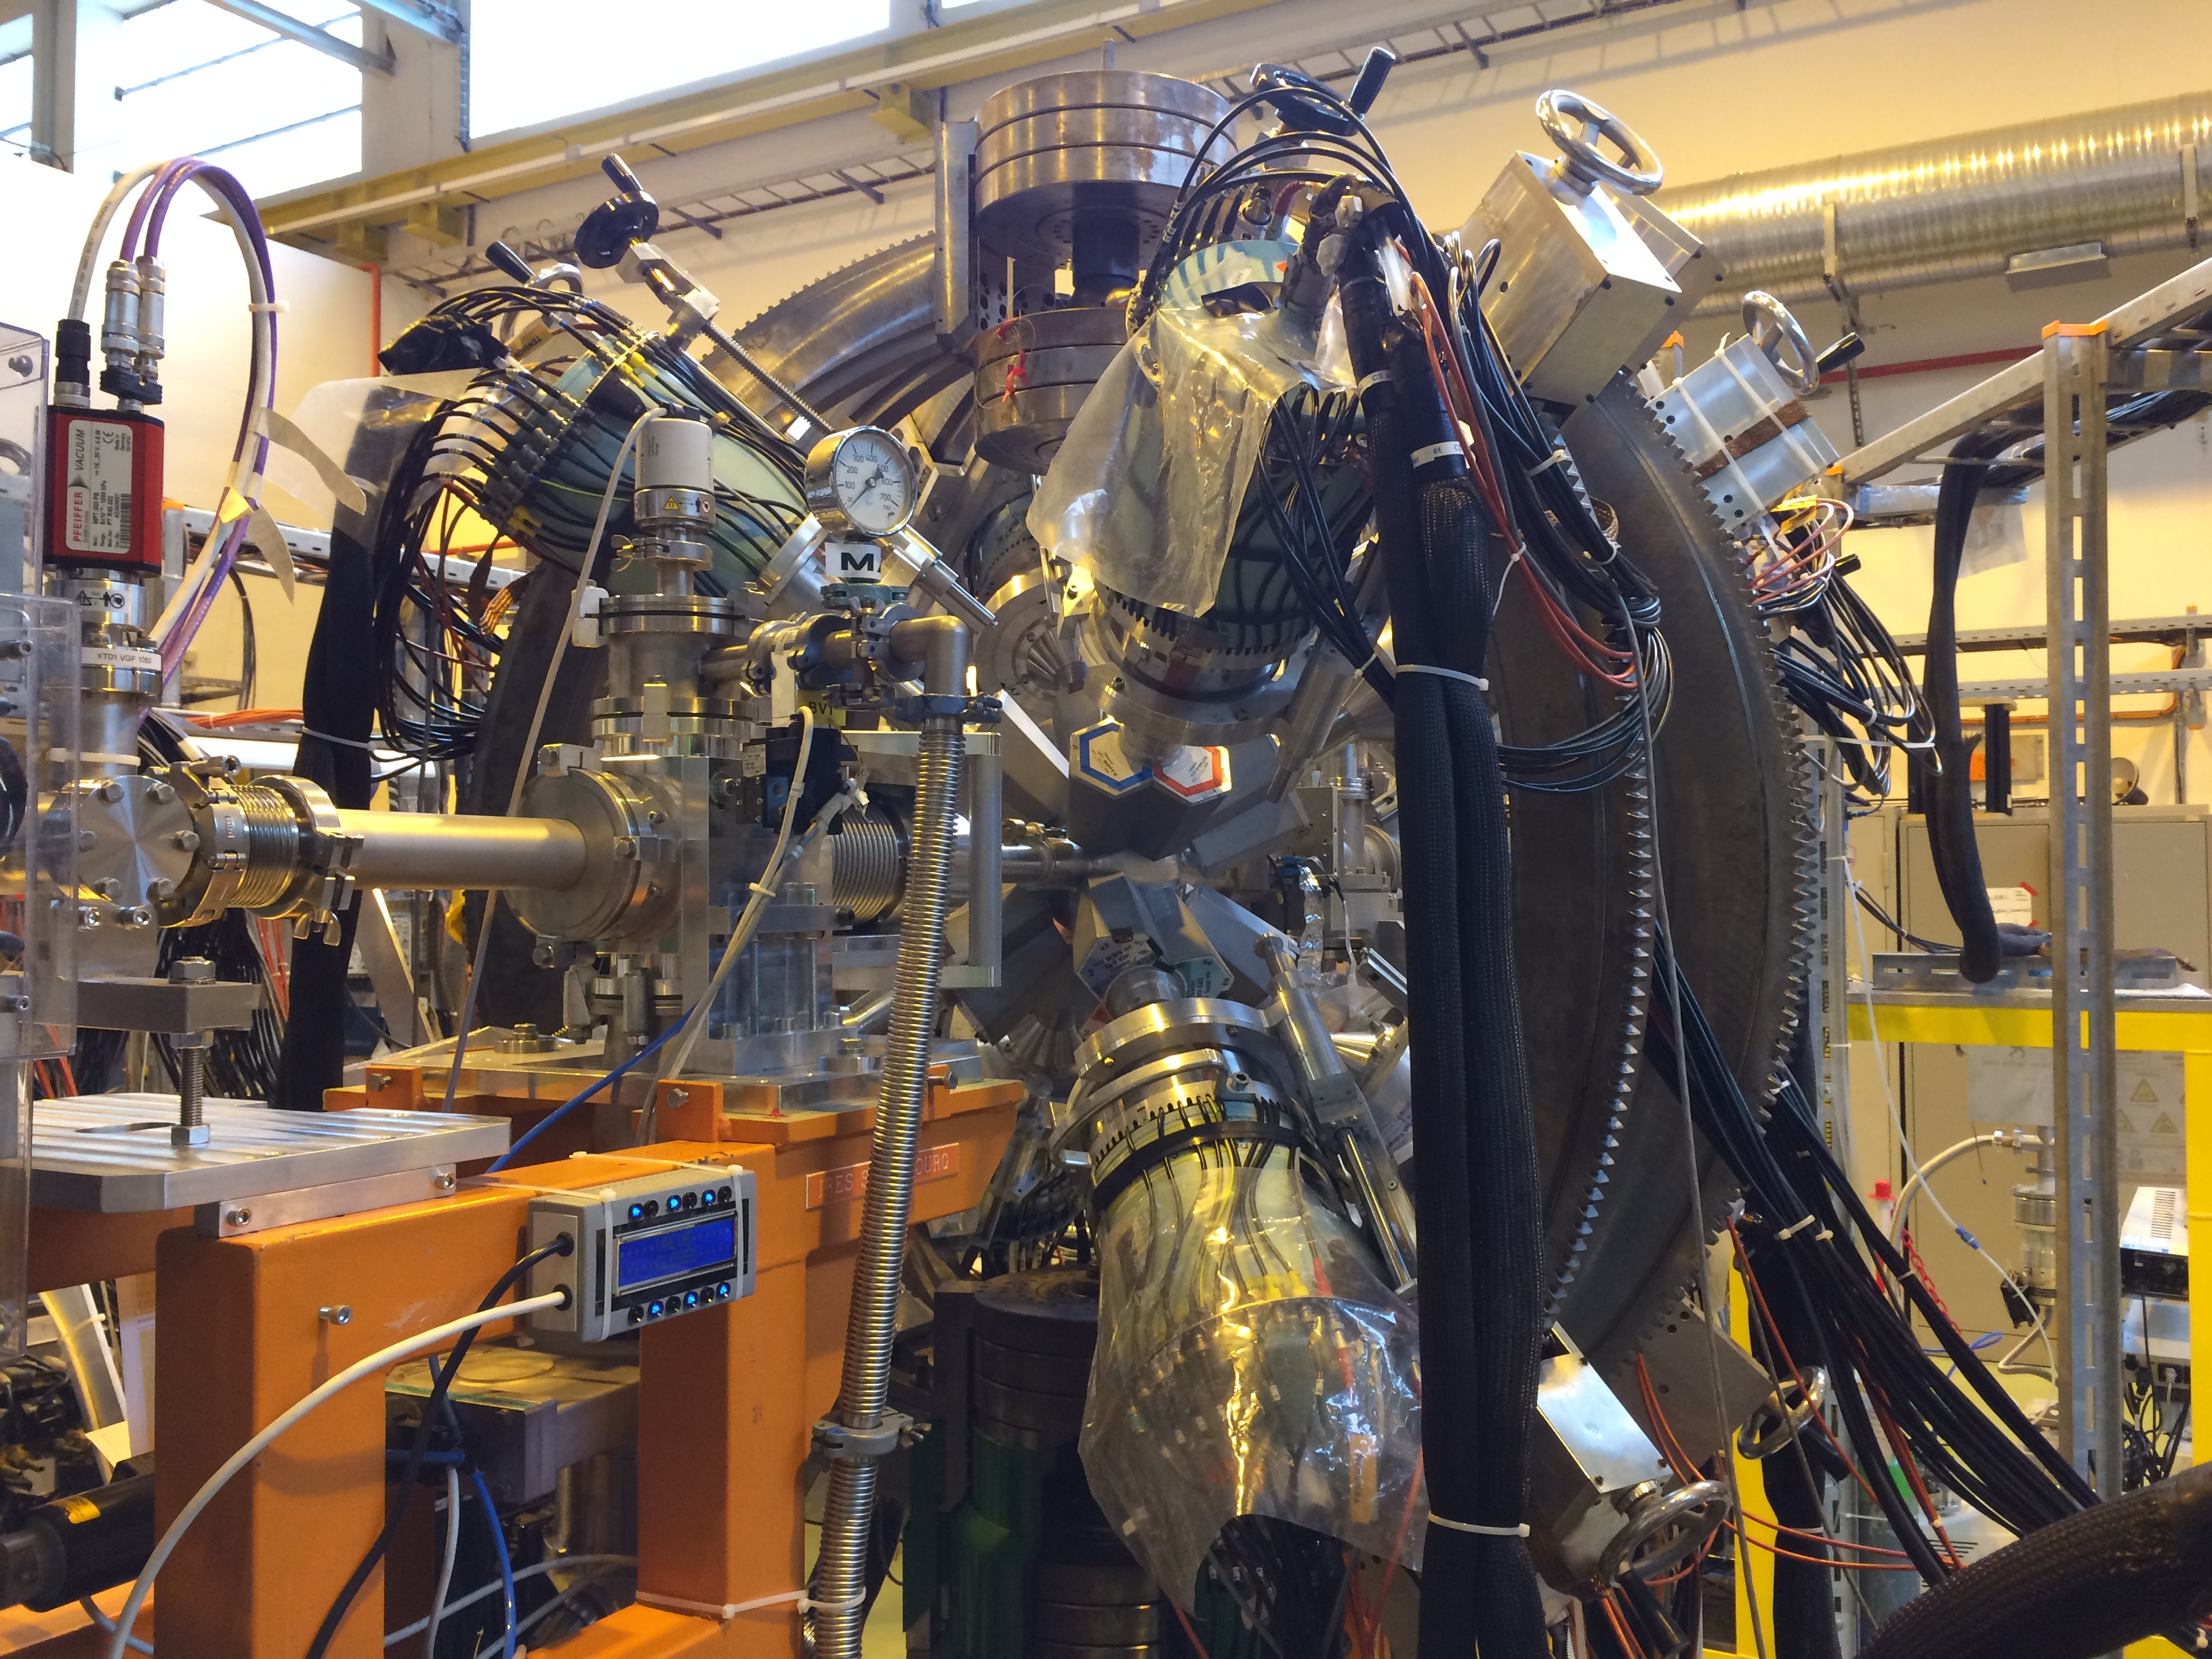
\includegraphics[width=\linewidth]{Images/IMG3849.JPG}
	\caption{An overview picture of the Miniball spectrometer. The target chamber is in the middle of the picture, surrounded by the \ga\ detector array. Photo by: Trond Wiggo Johansen.}
	\label{fig:MBSpect}
\end{figure}


\subsubsection{Target chamber}
The target chamber is a hollow sphere made out of a machined out, single piece of aluminium alloy (AlMg$_3$), with a thin wall and an inner radius of approximately 80 mm. 
Inside the chamber we find a target wheel and a particle detector. 
As shown in \autoref{fig:TWheel}, the target wheel can hold up to six different targets. 
The particle detector can be positioned 25 - 31 mm from the target wheel, limited by the space inside the chamber. 
Outside of the target chamber, the average distance from each \ga\ detector cluster to the center of the target chamber is approximately 10 cm.
The forward and the backward \ga\ detector clusters are placed in a 45$^\circ$ and 135$^\circ$ angle $\theta$, respectively, compared to the beam line.
In the vertical plane, perpendicular to the beam line, the four \ga\ detector clusters in forward and backward position are placed roughly on a circle with a separation of $\phi = 90^\circ$ \cite{MB-spect}.  

\begin{figure}[ht]
	\centering
	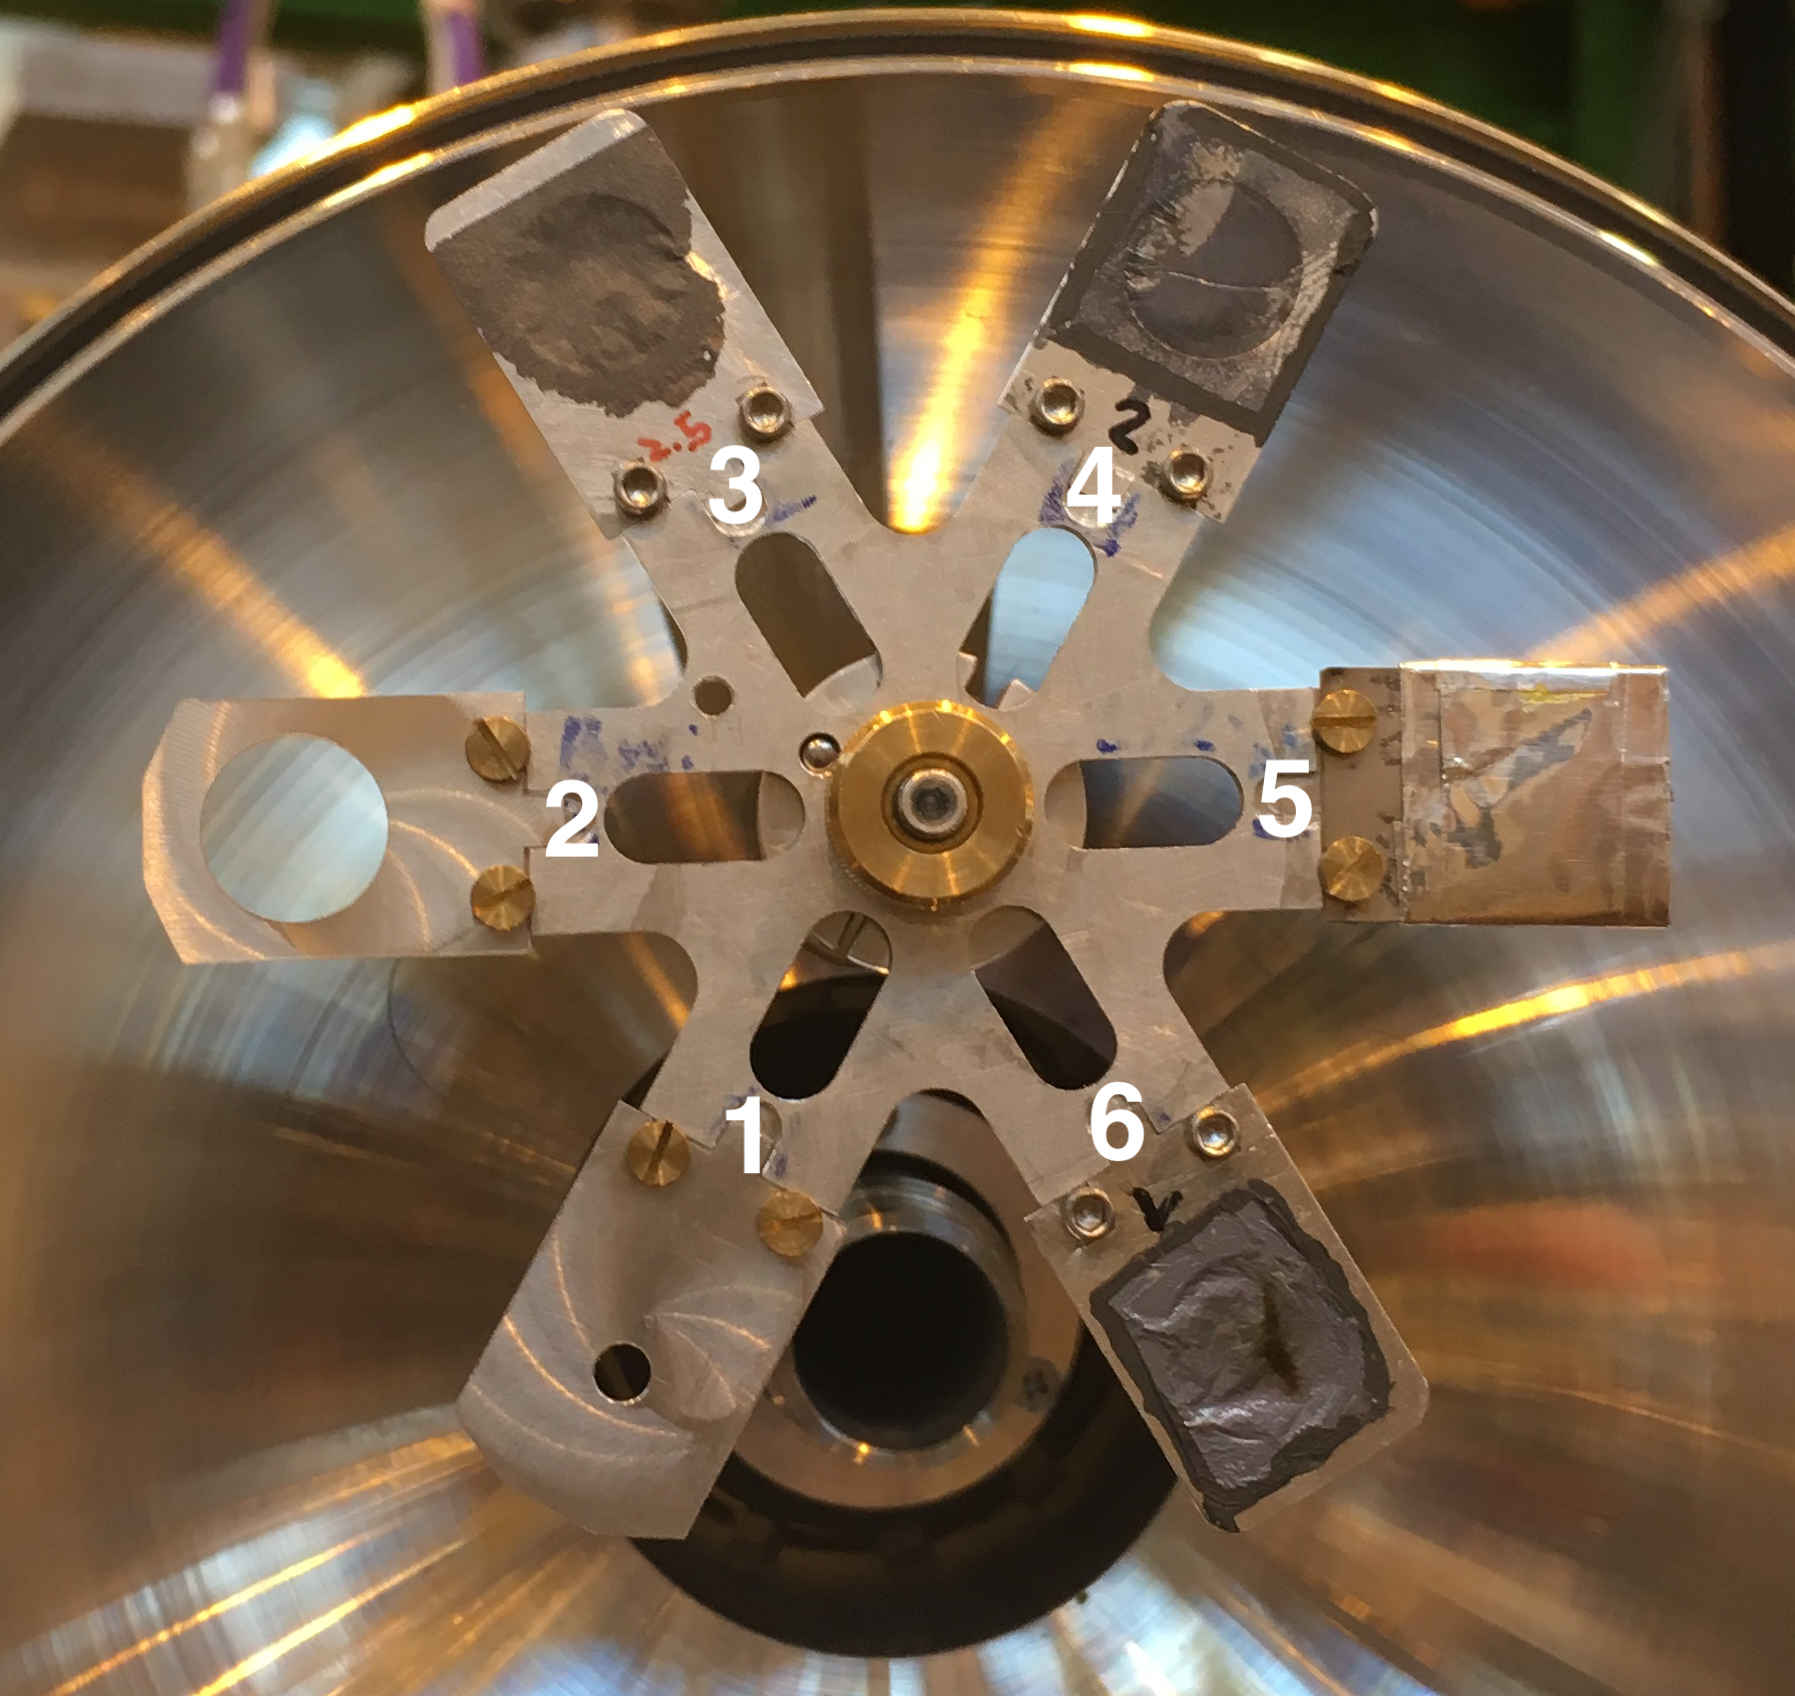
\includegraphics[width=0.8\linewidth]{Images/Target-wheel.png}
	\caption{The target wheel can hold up to six different targets. Position 1 and 2 are holes with a diameter of 3 and 12 mm respectively. They are used for beam tuning. Position 3 and 4 has \Pb\ targets with thickness 2.5 and 0.7 mg/cm$^2$ respectively. Position 5 has 13 layers of $^{27}$Al foil. Position 6 has the target \Pb\ with thickness 1.4 mg/cm$^2$, which was the secondary target used in the present experiment. Photo by: Dr. Liam Gaffney, date: 07.08.2017.}
	\label{fig:TWheel}
\end{figure}


\subsubsection{Particle detector, DSSSD (CD)}
To detect the scattered beam and target nuclei, a segmented Double Sided Silicon Strip Detector (DSSSD) composed of four quadrants was used. 
\autoref{fig:CD-FB} shows a sketch of the front and back of the detector. 
The DSSSD resembles an audio Compact Disc (CD), and hence it is called the CD. 
In the front of the CD, one quadrant consists of 16 annular strips (rings) with a pitch of 2 mm, while the back consists of 24 sector (radial) strips with a pitch of 3.5$^\circ$. 
The innermost strip has an inner radius of the active area of 9 mm, while the outermost strip has an outer radius of the active area of 40.9 mm. 
The active area of the detector is the area in which a particle can be detected, the detectable surface. 

In total, there are 160 discrete detector elements for all four quadrants, 64 in front and 96 in back. 
Each quadrant of the CD is independently connected to a Analog to Digital Converter (ADC) and a Time to Digital Converter (TDC). 
The TDC keeps track of the time of registered particle-\ga\ and particle-\ga-\ga\ coincidences. 
As a result of too few available channels in the ADC, the sector strips in the back are paired up.
In consequence, it is effectively 12 strips on the back side of the CD. 

The whole CD detector has a total area of 5000 mm$^2$, where approximately 93$\%$ of the detector consists of a detectable surface. 
In Coulomb excitation experiments the silicon wafer thickness is usually 500 $\mu$m.
The silicon wafer is the thin slice of semiconductor which can detect the incoming particles. 
For simplicity the dead layer thickness is usually assumed to be 0.7 $\mu$m \cite{NWarr-CD, MB-spect}. 
\autoref{tab:CD_spec} shows some of the specifications of the CD.  
The distance from the target to the CD was 27 $\pm$ 1 mm. 
In the laboratory (LAB) reference frame the CD covers an angle range between 18.4$^\circ$ and 56.6$^\circ$. 
The angles are divided up in rings corresponding to the scattering angles in \autoref{tab:scattering}.
An extensive description of the CD can be found in \cite{CD-DSSSD}.

%\footnote{The distance was measured using a $\alpha$-source ($^{226}$Ra). The source has a thickness of 1.23 mm, which has to be accounted for. The target to CD distance is therefore the CD to source distance plus the source thickness, i.e. 25.78(12) mm + 1.23 mm = 27.01 mm. This source data was reanalyzed, giving a 0.03 mm discrepancy form the original log entry. In private communications at ISOLDE in August 2018, the distance from the target to the CD was determined to be 26.98 mm with a $\sim$1 mm uncertainty.}

\begin{figure}[htb]
	\centering
	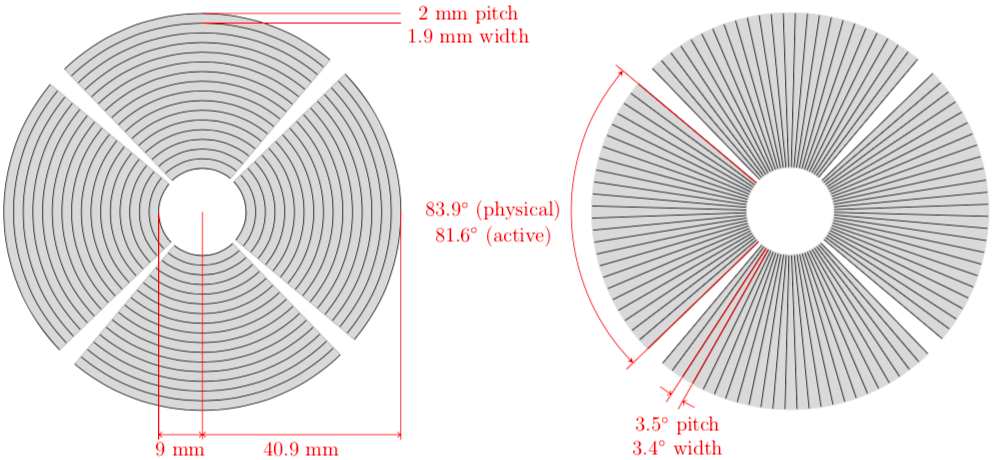
\includegraphics[width=\linewidth]{Images/CD.png}
	\caption{CD sketch, adapted from \cite{NWarr-CD}. 
	On the left is the front side of the CD. 
	The beam goes into the paper from the perspective of the left drawing.
	Front (annular) strips are numbered from 0 (outermost) to 15 (innermost). 
	Quadrants are numbered in clockwise direction with respect to the beam direction, which corresponds to: left is 1, up is 2, right is 3 and down is 4.
	On the right is the back side of the CD. 
	The beam comes out of the paper from the perspective of the right drawing.
	Back (radial) strips are numbered from 0 to 23 in counter-clockwise direction.
	Viewed from this perspective, the quadrants are numbered as: right is 1, up is 2, left is 3 and down is 4.}
	\label{fig:CD-FB}
\end{figure}

\begin{table}[htb] 
    \centering 
    \caption{CD specifications.}
	% Data for the CD specification table
\begin{tabular}{lll}
\hline
                            & Annular strips & Secular strips \\
                            & (CD Front)     & (CD Back)      \\
\hline
Number of strips            & 16             & 24             \\
Inner radius of active area &  9.000 mm      & -              \\
Outer radius of active area & 40.900 mm      & -              \\
Strip pitch                 &  2.000 mm      & 3.5$^\circ$    \\
Strip width                 &  1.900 mm      & 3.4$^\circ$    \\
Strip length                &  -             & 31.900 mm      \\
Active angle coverage       & 81.6$^\circ$   & 81.6$^\circ$   \\
Inner strip distance        &  -             & 0.100 mm       \\
\hline
\end{tabular}
	\label{tab:CD_spec}
\end{table}

\begin{table}[htb] 
    \centering 
    \caption{Scattering of \Sm\ on \Pb\ with beam energy 4.65 MeV/u.
    Calculations are done with the LISE++ \cite{LISE} kinematics calculator with a reaction from the middle of the target.
    The LAB and CM frame angles are based on the LAB input angles from $\theta_b$ and $\theta_t$. 
    In \textbf{(b)} there are angles marked with red color. 
    These are overlapping with the CM angles in \textbf{(a)}, making a total of 24 unique angles in the CM frame marked in black.}
	\label{tab:scattering}
    \begin{subtable}{0.45\textwidth}
    		\centering
		\caption{$\theta_b \in [22.0^\circ, 56.7^\circ]$.}
	 	\label{tab:LABvsCM_b}
	 	% Data for the LAB vs CM angle table
\begin{tabular}{ccc}
\hline
\multicolumn{2}{c}{LAB} & CM  \\
$\theta_b$ [$^\circ$]   &  $\theta_t$ [$^\circ$]  &  $\theta_b^{'}$ [$^\circ$]  \\
\hline
22.0                    &  71.7                   &  36.6                       \\
26.0                    &  68.4                   &  43.2                       \\
29.1                    &  65.9                   &  48.2                       \\
32.2                    &  63.4                   &  53.3                       \\
35.2                    &  60.9                   &  58.1                       \\
37.9                    &  58.8                   &  62.4                       \\
40.4                    &  56.8                   &  66.3                       \\
42.8                    &  54.9                   &  70.1                       \\
45.0                    &  53.2                   &  73.5                       \\
47.1                    &  51.6                   &  76.7                       \\
49.0                    &  50.2                   &  79.6                       \\
50.7                    &  48.9                   &  82.1                       \\
52.4                    &  47.6                   &  84.7                       \\
53.9                    &  46.5                   &  86.9                       \\
55.3                    &  45.5                   &  88.9                       \\
56.7                    &  44.5                   &  91.0                       \\
\hline
\end{tabular}
	\end{subtable}
	\begin{subtable}{0.45\textwidth}
		\centering
		\caption{$\theta_t \in [22.0^\circ, 56.7^\circ]$.}
		\label{tab:LABvsCM_t}
		% Data for the LAB vs CM angle table
\begin{tabular}{ccc}
\hline
\multicolumn{2}{c}{LAB} & CM  \\
$\theta_b$ [$^\circ$]   &  $\theta_t$ [$^\circ$]  &  $\theta_b^{'}$ [$^\circ$]  \\
\hline
{\color{red}40.6}  &  {\color{red}56.7}  &  {\color{red}66.6}   \\
{\color{red}42.3}  &  {\color{red}55.3}  &  {\color{red}69.4}   \\
{\color{red}44.2}  &  {\color{red}53.9}  &  {\color{red}72.2}   \\
{\color{red}46.1}  &  {\color{red}52.4}  &  {\color{red}75.2}   \\
{\color{red}48.3}  &  {\color{red}50.7}  &  {\color{red}78.6}   \\
{\color{red}50.6}  &  {\color{red}49.0}  &  {\color{red}82.0}   \\
{\color{red}53.1}  &  {\color{red}47.1}  &  {\color{red}85.8}   \\
{\color{red}56.0}  &  {\color{red}45.0}  &  {\color{red}90.0}   \\
			59.1   &  			  42.8   &  		    94.4    \\
		    62.5   &  			  40.4   &  		    99.2    \\
		    66.1   &  			  37.9   &  		    104.2   \\
		    70.2   &  			  35.2   &  		    109.6   \\
		    75.0   &  			  32.2   &  		    115.6   \\
		    80.2   &  			  29.1   &  		    121.8   \\
		    85.8   &  			  26.0   &  		    128.0   \\
		    93.8   &  			  22.0   &  		    136.0   \\
\hline
\end{tabular}

	\end{subtable}
\end{table}


\subsubsection{The high-purity germanium (HPGe) \texorpdfstring{$\gamma$}{Gamma} detectors}
In Coulomb excitation experiments, the target chamber is surrounded by the \ga\ detectors as displayed in \autoref{fig:MBSpectCU}. 
The \ga-ray spectrometer consists of a total of 24 six-fold segmented High-Purity Germanium (HPGe) crystals, which are divided into 8 clusters of 3 crystals each. 
Each crystal is encapsulated and segmented into 6 parts, making a total of 144 segments. 
Compared to using the whole crystal, a better Doppler correction can be performed when the \ga\ detectors are segmented. 

\begin{figure}[ht]
	\centering
	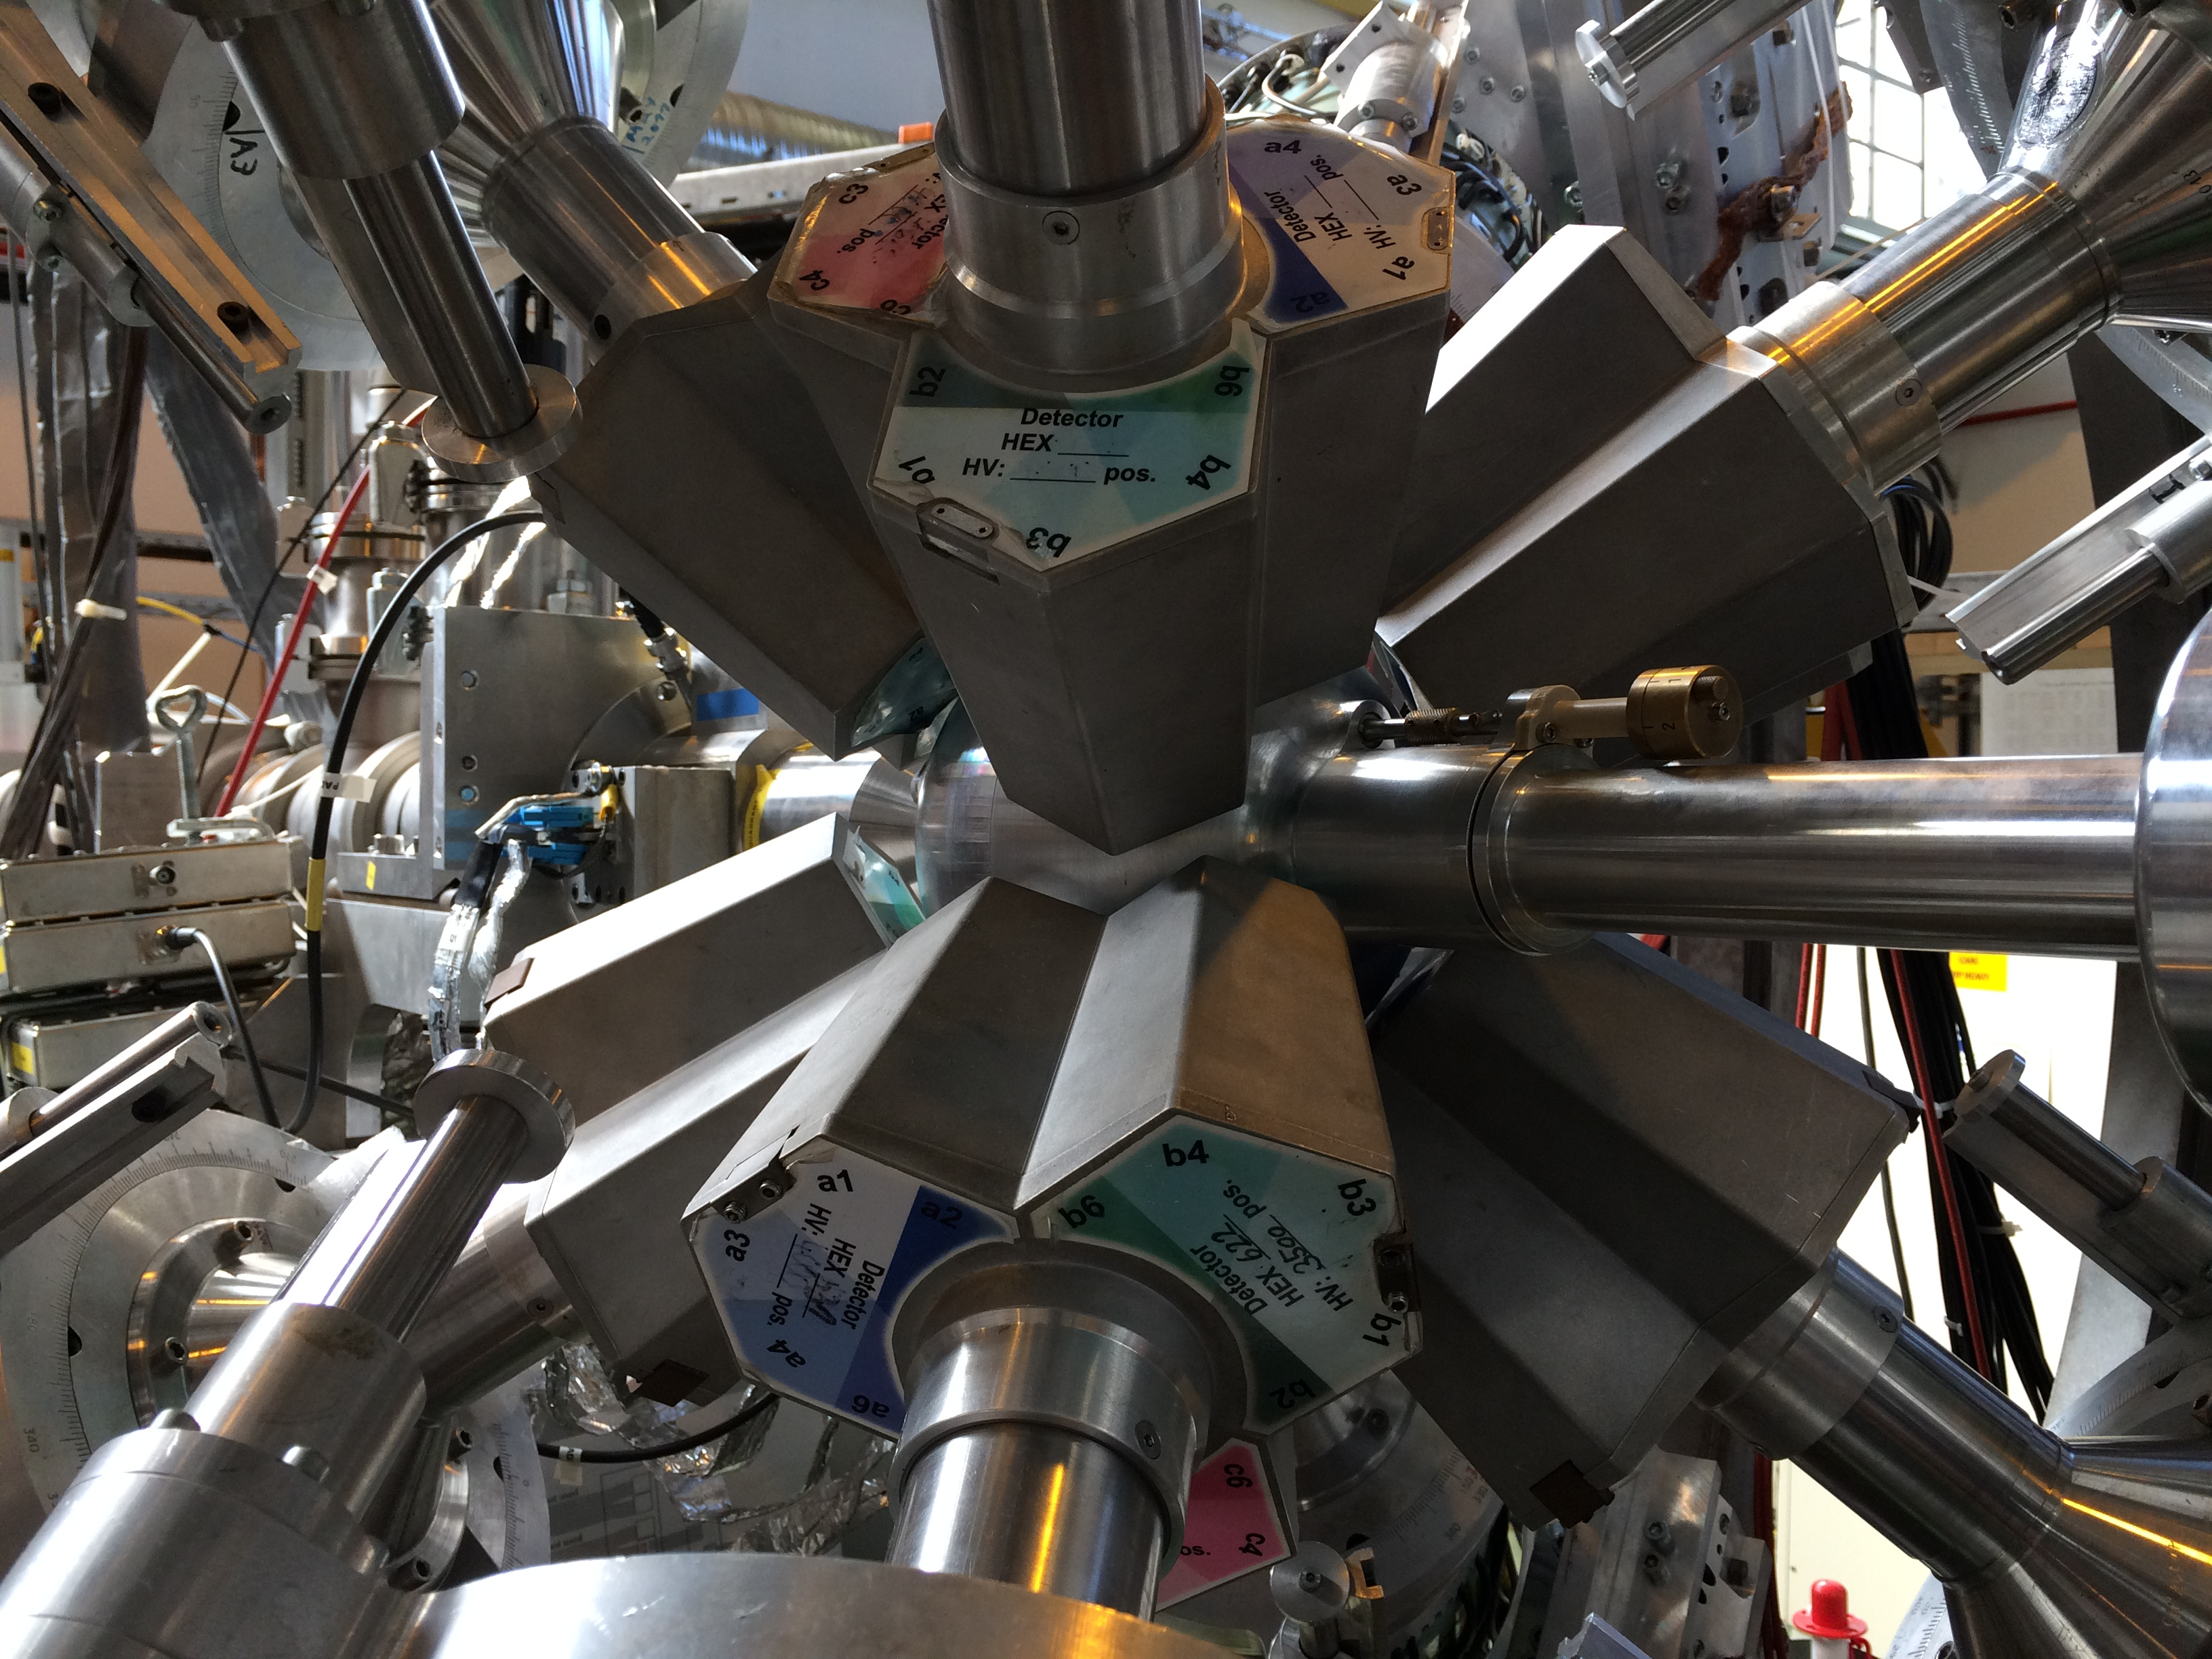
\includegraphics[width=\linewidth]{Images/IMG3917.JPG}
	\caption{Close up picture of the Miniball spectrometer. The Miniball target chamber is in the middle, surrounded by the triple-cluster encapsulated \ga\ crystals. The beam line goes through the target chamber. \\ Photo by: Trond Wiggo Johansen.}
	\label{fig:MBSpectCU}
\end{figure}

For maximum efficiency, the detectors are placed in a compact geometry around the target chamber \cite{NWarr-HPGe, MB-spect}. 
The detector-array can cover a solid angle of about 60\% of 4$\pi$, when the optimum distance between the target chamber and the HPGe clusters is achieved. 
The average energy resolution at $E_\gamma = 1.3$ MeV is 2.3 keV \cite{Butler2017}. 
During operation the HPGe clusters needs to be cooled down by liquid nitrogen which is provided by the automated filling system. 

\autoref{fig:HPGe} shows a sketch of one triple-cluster of the HPGe \ga\ detector array, with the corresponding table of all of the clusters positions.
From each detector we get seven signals in total for each event, one from the core and six from each segment. 
This requires 168 channels for data acquisition. 
The shapes of these signals are analyzed to provide information about the energy and time of the \ga-ray, in addition to the detection position within the detector cluster \cite{NWarr-HPGe}.

\begin{figure}[ht]
	\centering
	\begin{subfigure}[b]{0.49\textwidth}
		\centering
		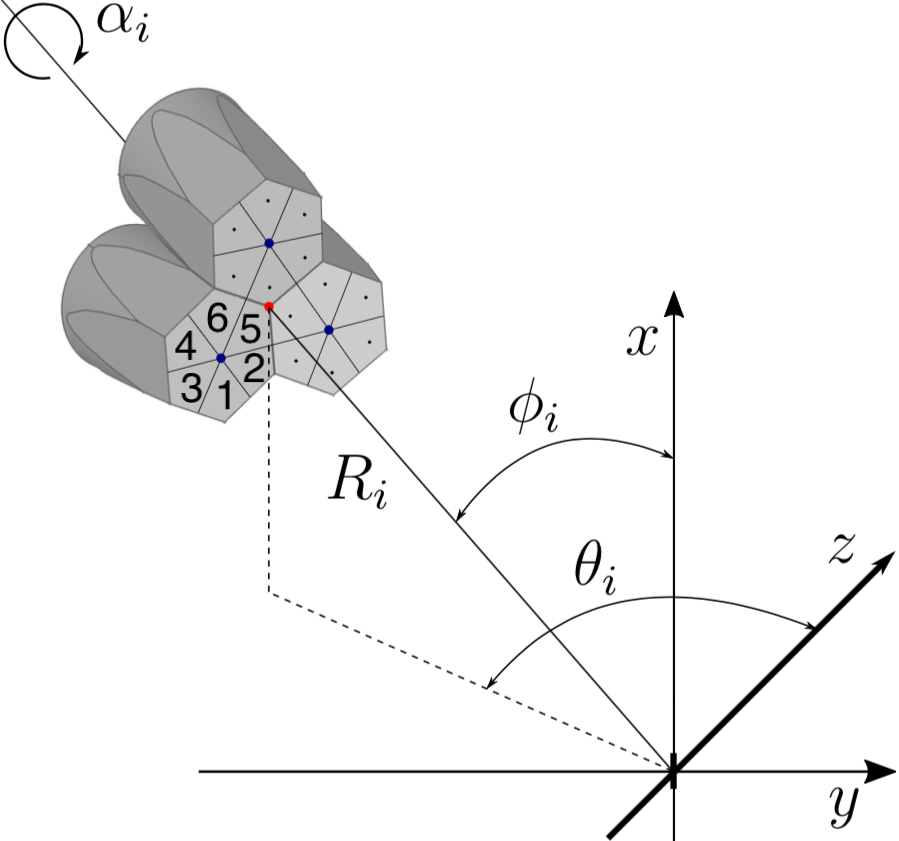
\includegraphics[width=\textwidth]{Images/HPGe2.png}
	\end{subfigure}
	\hfill
	\begin{subfigure}[b]{0.49\textwidth}
		\centering
    		% Data for the Geometry table
\caption{Geometry}
\label{tab:Geo}
\begin{tabular}{ccccc}
\hline
Cluster  &  $\theta$ [$^\circ$]  &  $\phi$ [$^\circ$]  &  $\alpha$ [$^\circ$]  &  R [mm]  \\
\hline
0        &  311.16               &  126.67             &  129.79               &  107.08  \\
1        &  51.08                &  62.74              &  51.83                &  100.59  \\
2        &  309.02               &  126.87             &  51.23                &  105.76  \\
3        &  251.90               &  57.44              &  130.31               &  105.40  \\
4        &  296.93               &  235.53             &  128.74               &  106.48  \\
5        &  233.45               &  239.09             &  46.67                &  105.18  \\
6        &  59.42                &  308.67             &  131.04               &  127.04  \\
7        &  130.56               &  309.09             &  46.46                &  110.18  \\
\hline
\end{tabular}
 \newline % newline lifts the table up one line
	\end{subfigure}
	\caption{On the left is a sketch of the HPGe triple-cluster position, adapted from \cite{Rosiak}. 
	Each cluster is segmented into 6 parts. 
	The core signal is marked by the blue dots in the middle of each of the three crystals, and the center of the triple-cluster is marked with a red dot. 
	There are four parameters, $\theta_i$, $\phi_i$, $\alpha_i$ and $R_i$, to determine the position of one triple-cluster.
	The angles, $\theta_i$ and $\phi_i$, are defined from a right-hand polar coordinate system, as displayed by the sketch.
	$\alpha_i$ determines the clockwise rotation around the center of the triple-cluster as seen from the target position.
	$R_i$ is the distance from the middle of the target chamber to the center of one triple-cluster.
	In the sketch, the secondary target is positioned in origo and the beam direction goes along the $z$-axis \cite{NWarr-Angles, Rosiak}. 
	On the right side is a table which contains the HPGe triple-cluster parameters for the present experiment, where $i$ denotes the cluster number used in the Miniball setup. 
	The geometry is used for the Doppler correction, which is discussed in \autoref{ssec:Doppler}.}
	\label{fig:HPGe}
\end{figure}


\section{The data acquisition system}\label{sec:DAQ}
Signals from the CD and the HPGe clusters are read out by the ADC, TDC and Digital Gamma Finder (DGF) modules and sent to a Personal Computer (PC) in the Data AcQuisition (DAQ) room at ISOLDE. 
The data is then stored in a PC. 
The ADCs and DGFs record an energy and a time-stamp with 25 ns ticks. 
It is the multiplicity of the output of the DGFs that is used to generate the \ga\ signal, which in turn is used to make the particle-\ga\ coincidence.

The collection of data is done by the \MBOU\ \cite{Maraboou, Maraboou-web} DAQ system \cite{MB-spect}. 
It is split in two parts, as presented in \autoref{fig:MARaBOOU}, one front-end part based on the Multi Branch System (MBS) \cite{MBS} and one back-end part based on the ROOT framework \cite{ROOT}.
The front-end takes care of data readout, event building and data transportation, while the back-end takes care of the setup, run control, histogramming, data analysis and data storage. 

The system can manage high counting rates without much dead time. 
For a detection system, the dead time is the time after a readout of events where the system is unable to record another event. 
The ADCs and TDCs can buffer up to 32 events at a time \cite{MB-spect}. 
Essentially, the largest limitation to the DAQ system is pile-up, which is when the detection system starts processing another event before the previous event was finished. 
The events adds on top of each other, which leads to loss of information from both events.

During an experiment, the ROOT back end is mostly used to inspect the experiment live. 
As will be detailed in \autoref{ch:DA}, the offline ROOT analysis is very time consuming, and is largely performed after the experiment. 
This is the main part of the thesis.

\begin{figure}[ht]
	\centering
	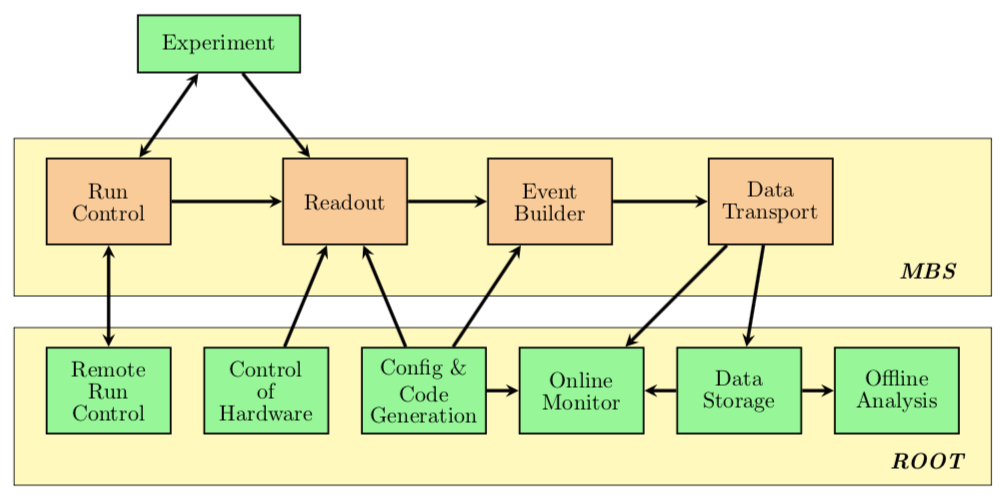
\includegraphics[width=\linewidth]{Images/MARaBOOU.png}
	\caption{\protect\MBOU\ tasks, adapted from \cite{Maraboou}.}
	\label{fig:MARaBOOU}
\end{figure}


\section{The time structure}\label{sec:time_structure}
In \autoref{fig:ITS}, a schematic of the ISOLDE time structure is displayed. 
The Miniball data acquisition occurs during two time windows, the "on-beam" and "off-beam" windows. 
When REXEBIS releases the beam to the HIE-ISOLDE LINAC, a signal to generate the on-beam window is sent. 
This window, called the "slow extraction mode" was 800 $\mu$s, but in 2011 it was extended to 1 ms, as the beam extraction method was improved. 
All the data are read out after the on-beam window. 
During a readout, the DAQ becomes dead for a little while, so the next window is triggered when the DAQ is operable again.
The off-beam window starts 60 $\mu$s after the end of a readout of the on-beam window.
This allow the ADCs and TDCs time to start again.
The time structure of ISOLDE makes it possible to record data again in the off-beam window, before the next beam bunch is sent from REXEBIS.
In the off-beam window, which has the same duration of time as the on-beam window, data recordings of the background is conducted.
After the off-beam window closes, a readout of the records is triggered.
It is then possible to subtract the off-beam window from the on-beam, obtaining only the beam contribution. 
The next on-beam window is triggered when the DAQ is operable again.
The DAQ system records the signals from each detector segment, which is individually time-stamped. 
With these records, a full reconstruction of the real events and coincidences are possible \cite{NWarr-el}. 

\begin{figure}[ht]
	\centering
	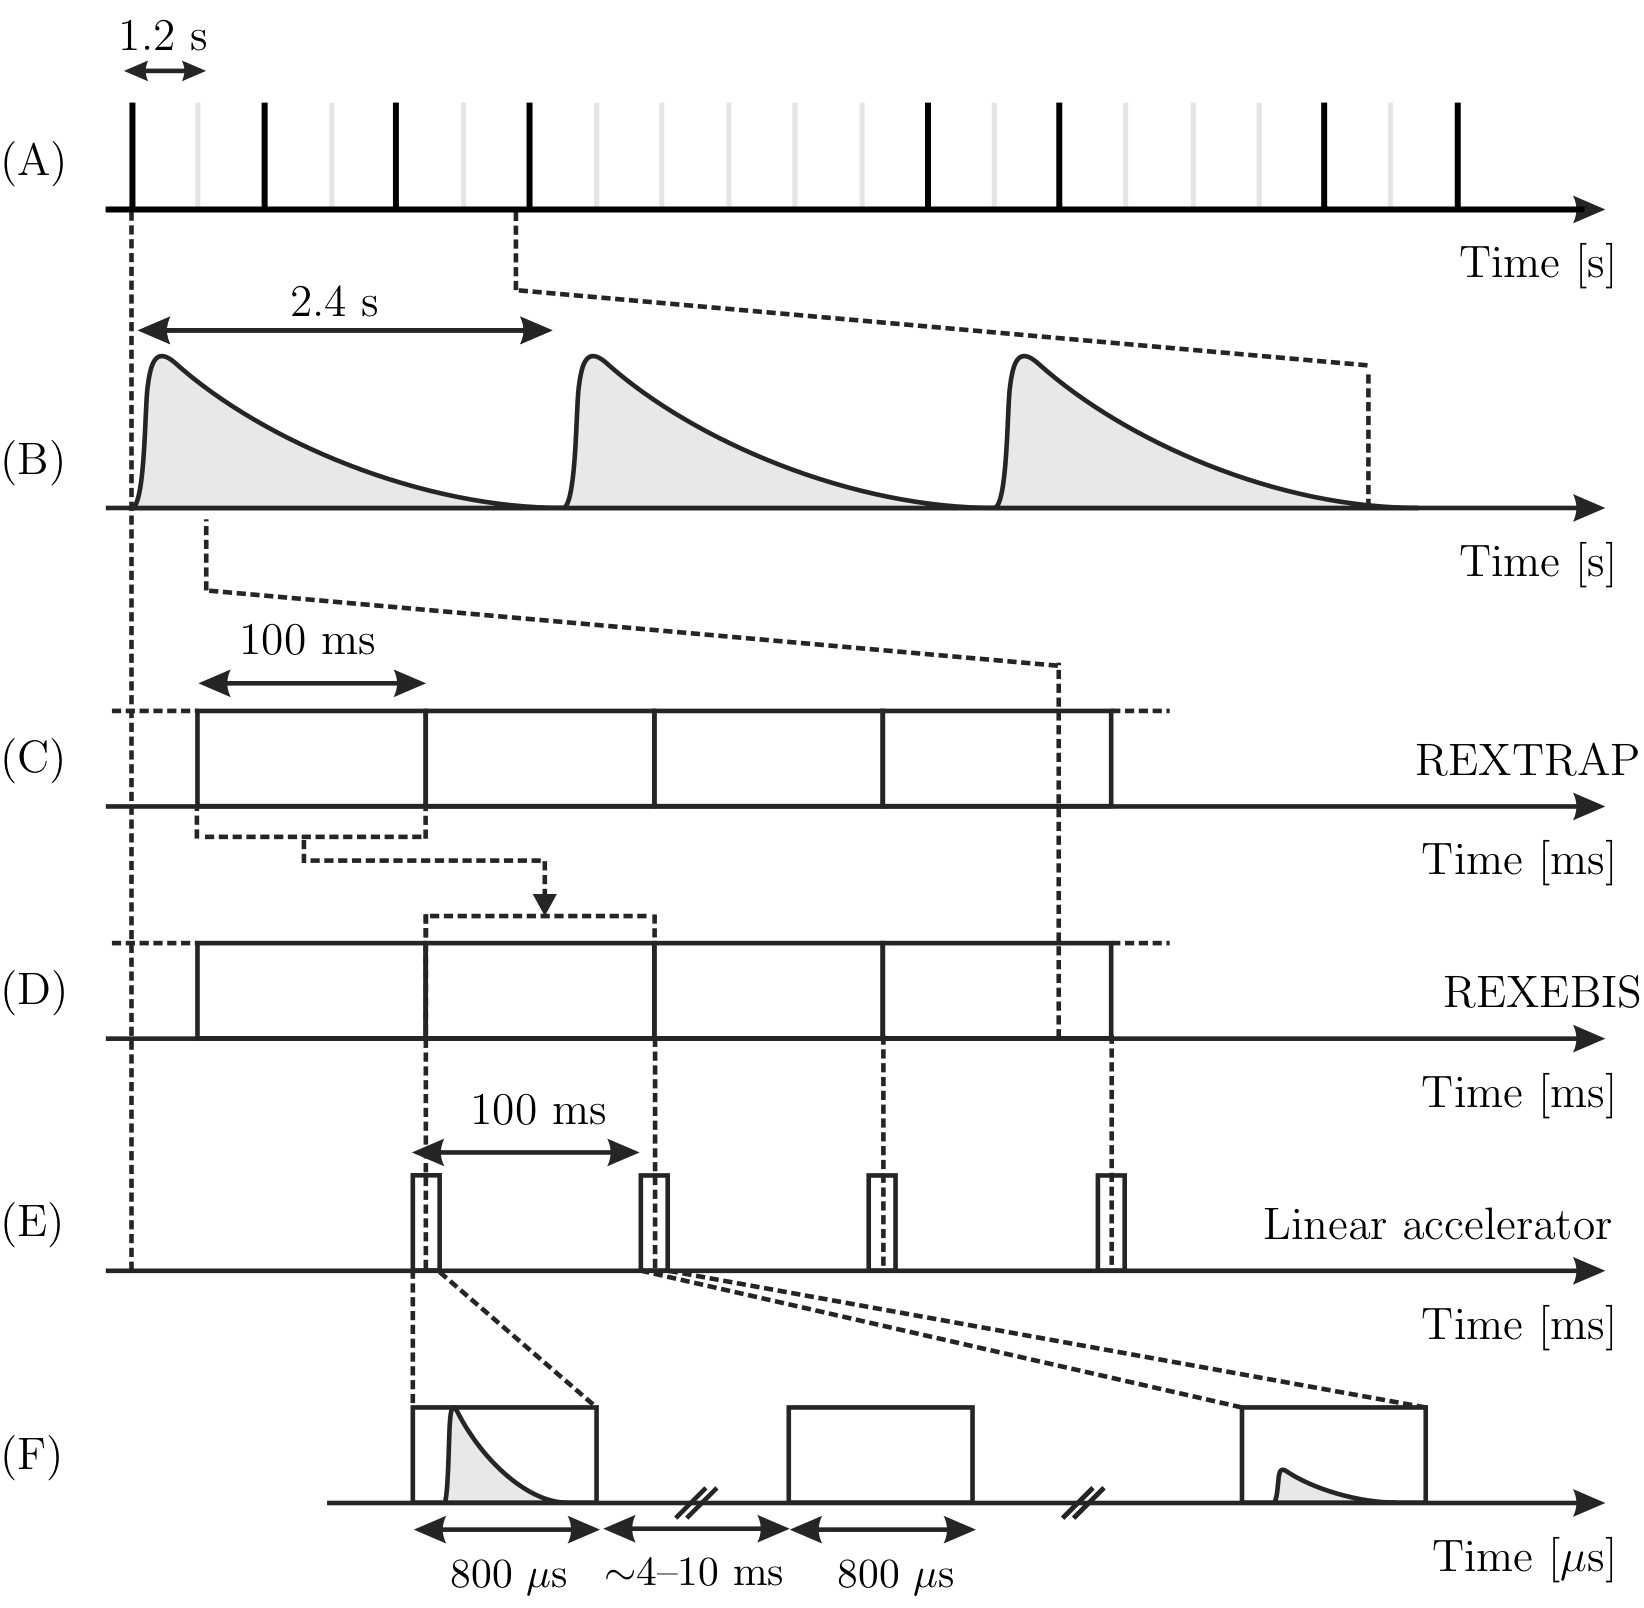
\includegraphics[width=0.8\textwidth]{Images/Time-structure.png}
	\caption{Schematic of the ISOLDE time structure, from \cite{Gaffney}. Figure courtesy of J. van de Walle \cite{HI-TDR}. (A) The supercycle of proton beam bunches with a width of $\approx 100 ~\mu$s from the PSB separated by 1.2 s. The black vertical lines shows an allocation of the the bunches which the ISOLDE production target receives, while the others are distributed to other experiments. (B) The release profile of radionuclides from the production target, which is heavily modulated by the PSB cycle. (C+D) REXTRAP and REXEBIS beam bunches, synchronized with (E) the radio frequency (RF) window of the HIE-ISOLDE LINAC. (F) The "on-beam" and "off-beam" time window of 800 $\mu$s using the Miniball setup.}
	\label{fig:ITS}
\end{figure}


% ----------------------------------------------------------------------------------------------------------------------% ----------------------------------------------------------------------------------------------------------------------


\chapter{Data analysis}\label{ch:DA}
\epigraph{\textit{"Not everything that can be counted counts, and not everything that counts can be counted."}}{\textit{– William Bruce Cameron}}


In this chapter, the general methods of the calibration and data analysis will be outlined. In addition, the various programs and scripts applied in the detector calibration and data analysis will be introduced. 
Scripts developed in the present thesis work for the fitting procedures were inspired by scripts written by Ville Virtanen\footnote{Ville Virtanen is a student from University of Jyväskylä.} and Dr. Liam Gaffney\footnote{Dr. Liam Gaffney is a research fellow at ISOLDE, affiliated with Miniball.}. 
The codes have been further developed and heavily re-written in the current work. 
Presently, the code has only a minor resemblance to the original code. 
The remaining Python and bash scripts are written and developed by the author.
All of the scripts written in C/C++ are dependent on the ROOT 6 framework \cite{ROOT}, a C/C++ data analysis framework developed and maintained at CERN.

Information about the computer setup and environment used in this thesis can be found in \autoref{a:computer_environment}. In the appendix there is also a section containing the relative path of programs, scripts and files.
All scripts and programs developed in this work are available in the authors GitHub repository \cite{GH-repo}.


\section{Data handling}
The goal of the data analysis is to obtain Doppler-corrected \ga-spectra with various conditions on particles and angles, in order to analyze the Coulomb excitation of \Sm. 
Before the required information can be extracted from the experimental data, all of the particle and \ga-ray detectors have to be calibrated.
However, the calibration cannot be performed without proper data handling first.

As described in \autoref{sec:DAQ}, all of the information corresponding to the experiment are handled by the data acquisition and stored in large data files. 
Generally speaking, the raw data files from Miniball experiments are formatted in so-called "list mode", where every new line contains the identification, energy and time of one single event\footnote{In truth, the format contains more information, identifying where the particle and \ga-ray hit the detectors.}.
%The format is not entirely correct, since it has identification of where the particle and \ga\ hit. 
%A more detailed format is: identification, time, particle energy (front strip, back strip), \ga\ energy (cluster, crystal, segment), etc.
All of the experimental data is stored in \textit{.med}-files, also known as Miniball Event Data, with a standard file naming convention. 
For example, \textit{140Sm\_208Pb\_pos6\_xyz.med} is the file name for the current experiment. 
Here \textit{x}, \textit{y} and \textit{z} are numbers between 0 and 9 which together gives the run number of the data acquisition. 
The expression \textit{140Sm\_208Pb} refers to the beam and secondary target, and \textit{pos6} means that the target wheel uses position 6 for the secondary target, see \autoref{fig:TWheel}.
A general rule of the data acquisition is to split the data over several run files to limit the file size, and the probability of corrupt files or data loss.

For Miniball experimental data, the preferred sorting and analysis code is \textsl{MiniballCoulexSort} \cite{MBCS}.
The code has been developed by several contributors from the Miniball collaboration over the years. 
Unfortunately, both the procedure and the code is lacking documentation, making it quite time demanding to learn how to run the code and to understand how it works.
A goal of this thesis is to document and make the procedure more transparent.
Currently is \textsl{MiniballCoulexSort} under constant development at CERN-ISOLDE under the management of Dr. Liam Gaffney. 
The main steps of how to download, install\footnote{If the \textbf{make} step fails, try doing a \textbf{make clean} and then \textbf{make}. The program might think that it has already been built.} and use \textsl{MiniballCoulexSort} is outlined in the \textit{README.md} file in the GitHub repository of Miniball \cite{MBCS}. 
\textsl{MiniballCoulexSort} is written in C/C++ and depends on the ROOT framework. 

To get from the raw data to the Doppler-corrected \ga-spectra, the data analysis code is divided into a three step procedure which can be summarized by the following subroutines:

\begin{enumerate}
	\item \texttt{MedToRoot} converts the raw data files to ROOT format. This is discussed in  \autoref{sec:data_conversion}.
	\item \texttt{TreeBuilder} performs the event building by
		\begin{itemize}
			\item calibrating detectors and applying channel thresholds for the ADCs
			\item using particle-\ga\ coincidences (correlations), i.e. the code figures out which \ga\ belongs to which particle
			\item storing everything in a tree structure for easy access
		\end{itemize}
		This is discussed in \autoref{ssec:online_cal}.
	\item \texttt{CLXAna} applies the gates on the particles and performs the Doppler correction. This is discussed in \autoref{ssec:gamma}.
\end{enumerate}


\subsection{Counting and naming convention for particle detector calibration}
When analyzing data using the \textsl{MiniballCoulexSort} code, the user have to be aware of the numbering of the CD.
The numbering of the CD rings and strips are different in the various programs and scripts. 
Histograms sorted by \texttt{TreeBuilder}, discussed in \autoref{ssec:online_cal}, starts counting from 0 (outermost ring) to 15 (innermost ring) as showed in \autoref{fig:CD-FB}. 
\texttt{AQ4Sort}, discussed in \autoref{ssec:user_cal}, starts from 1 (outermost ring) to 16 (innermost ring), shifted by 1 unit compared to the \texttt{TreeBuilder} numbering.
The simulation program \texttt{kinsim3}, discussed in \autoref{ssec:kinsim}, counts from 1 (innermost ring) to 16 (outermost ring), the opposite of \texttt{AQ4Sort}. 
For calibrated spectra, \texttt{TreeBuilder} shows the energy in MeV, while \texttt{AQ4Sort} shows the energy in keV.
To avoid further confusion, this thesis will apply the numbering system of \texttt{kinsim3} for the front side of the CD.

For the back side of the CD is \texttt{TreeBuilder} sorting from 0 to 11 in clockwise direction, while \texttt{AQ4Sort} sorts from 1 to 12.
This thesis will apply the numbering system of \texttt{AQ4Sort} for the back side of the CD.

\autoref{tab:ADC} shows the signal cable wiring of the CD into the ADC. \textcolor{red}{Koble sammen med kap. 3 i steden for...}

\autoref{tab:TBvsAQ4} shows the chosen way of counting and the histogram naming from \texttt{TreeBuilder} and \texttt{AQ4Sort}.


\section{Data conversion}\label{sec:data_conversion}
In order to analyze the data with the ROOT framework, the data files have to be converted from the 
\textit{.med} format produced by \MBOU\ into the \textit{.root} format by using the \texttt{MedToRoot} program. 
To effectively convert all of the data files in one run, a bash script called \texttt{M2R.sh} was written.
It takes in a user defined number of files and converts all the files in one go by using \texttt{MedToRoot}.
\texttt{M2R.sh} takes the element name as command line argument\footnote{\texttt{M2R.sh} was intentionally developed to convert \textit{.med}-files from different experiments, so it is fairly simple to expand the script to sort other data sets.} and if no command line arguments are given, the script will print out an usage description.
An example of the terminal use including the output for the \textit{140Sm\_208Pb\_pos6\_0xy.med}-file with \textit{xyz = 008} is as follows: 

% Empty language = plain text
\begin{lstlisting}[language=]
$ cd ~/GitHub/MasterThesis/Scripts/sorting
$ ./M2R.sh Sm
opening file ../../Raw_data/Sm/140Sm_208Pb_pos6_008.med ...
EventBuffer::EventBuffer(GlobalSettings *)
Processing event number       0
Start trigger #14

Processing event number  130000
Stop trigger #15


Unpacked 132802 events:
wrong dgf hit pattern:                      0 ( 0.0 %)
wrong adc headers:                          0 ( 0.0 %)
# of overflows in adc channels:        599712 (451.6 %)
# of underflows in adc channels:            0 ( 0.0 %)
pattern unit mismatches:                    0 ( 0.0 %)

Number of ebis pulses:            66351
Number of t1 pulses:               2211
Number of supercycle pulses:        429
committed       1 243 951 987  bytes to tree tr, 'Tree for on beam data of Coulex setup@Miniball'
and                15 338 250  bytes to tree bg, 'Tree for on beam background data of Coulex setup@Miniball'
and               237 454 436  bytes to tree tr, 'Tree for off beam data of Coulex setup@Miniball'
wrote                  97 189  bytes to file ../../Raw_data/Sm/140Sm_208Pb_pos6_008_OnBeam.root 	=> compressed by a factor of 12799.3
,                      18 362  bytes to file ../../Raw_data/Sm/140Sm_208Pb_pos6_008_OnBeamBackground.root 	=> compressed by a factor of 835.3
,                      67 934  bytes to file ../../Raw_data/Sm/140Sm_208Pb_pos6_008_OffBeam.root 	=> compressed by a factor of 3495.4
and                    22 167  bytes to file ../../Raw_data/Sm/140Sm_208Pb_pos6_008_Scaler.root 	=> compressed by a factor of 2769.1
\end{lstlisting}

For each file converted with \texttt{MedToRoot}, the program creates four files with the naming convention
\begin{itemize}
	\item \textit{140Sm\_208Pb\_pos6\_xyz\_OnBeam.root} 
	\item \textit{140Sm\_208Pb\_pos6\_xyz\_OnBeamBackground.root}
	\item \textit{140Sm\_208Pb\_pos6\_xyz\_OffBeam.root}
	\item \textit{140Sm\_208Pb\_pos6\_xyz\_Scaler.root} 
\end{itemize}
where the file of interest is the first one. The \textit{OnBeam.root}-files are used in the sorting and event building with \texttt{TreeBuilder} and/or \texttt{AQ4Sort}.

The "on-beam" and "off-beam" files refers to the time structure explained in \autoref{sec:time_structure} which is connected with the beam production explained in \autoref{ssec:beam_prod}.
The ions are trapped and transferred to the REXEBIS where they are charge-bred.
REXEBIS releases the ions periodically into the HIE-ISOLDE LINAC where they are accelerated. 
This defines a time structure of the beam and therefore, the events contains a flag from REXEBIS.
If the REXEBIS flag is "off", then the event is inserted into the \textit{OffBeam.root}-file.
Flag "on" means, in principle, that beam is on, and a more narrow time window with respect to the REXEBIS pulse can be specified. 
If the flag is "on" and the event is inside the time window, the event is added to the \textit{OnBeam.root}-file.
Otherwise, if the REXEBIS flag is "on", but the time stamp is outside the window, the event gets sorted into the \textit{OnBeamBackground.root}-file.
The \textit{Scaler.root}-file are for monitoring the count rates in the individual detectors.



\section{Detector calibration}\label{sec:detector_cal}
%The general idea of the calibration is to make sure that the energy spectra of all the detectors present the same physical features.
%In other words, for the same kind of particles or \ga-rays hitting the same angle range of the detector, the energy distribution produced by a detector should be aligned into the same position as the other detectors.

Every detector channel, including its electronics\footnote{Electronics like pre-amplifiers, ADCs, etc.} is slightly different from the other channels. 
It is therefore necessary to calibrate each detector channel in both energy and time.
Calibration of the detectors minimize the measurement uncertainty by making sure the detectors are consistent with each other.
If the detectors are not properly calibrated, adding spectra from different detectors may cause unwanted effects. 
For example, the true full energy peak may appear wider if one of the spectra in the sum is shifted in energy compared to the other spectra.
By determining the centroids of peaks in every spectrum, and comparing these with theoretical values obtained by simulating the kinematics of the reaction and energy loss, linear calibration coefficients of the detectors can be obtained. 
In this context, the centroid\footnote{Normally, the centroid is only the maximum if the peak is symmetric.} of the energy peaks refer to the channel of maximum height in the histogram.

Both the particle and \ga\ detectors applied in this experiment are semiconductor detectors. 
%Except for silicon (as the CD), semiconductors generally require cooling to low temperatures before they can be operated. 
The basic principle of operation is that incoming ionizing radiation\footnote{For the CD, the ionizing radiation is the beam or target particles scattered from the reaction, while the ionizing radiation for the HPGe detectors is the high-energy photons (\ga) from de-excitation of the nuclei.} creates electron-hole pairs in the semi-conducting material which are then collected by an electric field. 
The number of electron-hole pairs are assumed to be proportional to the energy of the incoming radiation to the semiconductor \cite{WRLeo}. 
By applying this assumption we obtain a linear correlation between the energy $E$ of the particle (or \ga-ray) and the channel number $n$ of the ADC (or DGF)
\begin{equation}\label{eq:Ego}
	E = g \cdot n + a
\end{equation}
where $a$ is the offset in keV and $g$ is the gain in keV/$n$. 
The gain $g$ and the offset $a$ are the coefficients needed to perform the calibration.
From \autoref{eq:Ego}, the offset $a$ can easily be expressed as 
\begin{equation}\label{eq:offset}
	a = E - g \cdot n 
\end{equation}
To find the gain $g$, at least two measuring points are needed
\begin{align}\label{eq:gain}
	g &= \frac{E_2 - E_1}{n_2 - n_1}
\end{align}
where the peak energies, $E$, are obtained from a simulation of the Coulomb excitation experiment and the channel numbers, $n$, are obtained from the raw data of the experiment.
To improve the precision of the calibration coefficients, it is desirable to use several data points to obtain $g$ and $a$ by a linear regression.

\textcolor{red}{Forklar at kalib.koeff. kan variere med tiden.}

By including more than two centroids, it is possible to check for non-linearities or instabilities in time.

\subsection{Kinematic simulation}\label{ssec:kinsim}
To calibrate the data, we need to calculate the expected energy of the centroids of the peaks in the energy spectrum. 
This was done by simulating the experiment using the program \texttt{kinsim3} \cite{kinsim} written by Dr. Liam Gaffney. 
The purpose of the program is to obtain the kinematics of a Coulomb excitation experiment that utilizes the CD. 
The simulations calculate the theoretical predictions of the energy distribution of the peaks for each ring in the CD. 
\texttt{kinsim3} returns simulated spectra for the LAB and CM frame, in addition to every annular strip of the CD.
The simulated strip spectra of the CD are fitted, their energy centroids are collected and used in the calibration as explained in \autoref{ch:cd_sim}.

\textcolor{red}{Fiks dette når jeg har hjernekapasitet...}
A detailed explanation of the input parameters of \texttt{kinsim3} is in \autoref{ch:cd_sim}.

\autoref{ch:cd_sim} shows the simulated energy for each ring of the CD, in addition to the fitted peaks of each ring.
In the fitting of the simulated (synthetic) data from \texttt{kinsim3}, a Gaussian function with linear background was applied
\begin{equation}
	g(x) = c + sx + A e^{-\frac{1}{2}\left(\frac{x - \mu}{\sigma}\right)^2}
\end{equation}
where $x$ is the energy centroid, $c$ is the background constant, $s$ is the background slope, $A$ is the amplitude (Gauss constant), $\mu$ is the mean (expected energy value) and $\sigma$ is the standard deviation (Gauss width). 
\autoref{tab:CD_angles} shows the angles of the center of each CD ring in the LAB frame for the front of the CD. 
A general kinematics simulation in the LAB frame and the experimental particle spectra is shown in \autoref{fig:part_events}. 

\begin{table}[htb] 
    \centering 
    \caption{The angles of the center of each CD ring in the LAB frame, with a distance from the target to the CD of 27 mm. 
    Ring 1 is the innermost ring and ring 16 is the outermost ring. 
    The centroid energies originates from a simulation with \texttt{kinsim3}. 
    $E_t$ is the energy of the secondary target particle (Pb) and $E_b$ is the energy of the beam particle (Sm).}
	% Data for the CD angles table
\begin{tabular}{ccccc}
\hline
Ring   & \multicolumn{2}{c}{Center of CD ring}                            &             &             \\
number & \shortstack{Distance from \\ beam line [mm]}  & Angle [$^\circ$] & $E_t$ [MeV] & $E_b$ [MeV] \\
\hline
1      & 10                                            & 20.3             & 484.86      & 539.89      \\
2      & 12                                            & 24.0             & 457.53      & 520.55      \\
3      & 14                                            & 27.4             & 428.87      & 499.72      \\
4      & 16                                            & 30.7             & 398.95      & 478.33      \\
5      & 18                                            & 33.7             & 369.54      & 456.71      \\
6      & 20                                            & 36.5             & 340.64      & 435.42      \\
7      & 22                                            & 39.2             & 313.65      & 414.84      \\
8      & 24                                            & 41.6             & 287.31      & 395.31      \\
9      & 26                                            & 43.9             & 262.77      & 376.35      \\
10     & 28                                            & 46.0             & 240.36      & 358.75      \\
11     & 30                                            & 48.0             & 219.53      & 342.40      \\
12     & 32                                            & 49.8             & 198.95      & 326.87      \\
13     & 34                                            & 51.5             & 182.41      & 312.31      \\
14     & 36                                            & 53.1             & 164.55      & 299.11      \\
15     & 38                                            & 54.6             & 151.51      & 286.78      \\
16     & 40                                            & 56.0             & 139.62      & 273.80      \\
\hline
\end{tabular}
	\label{tab:CD_angles}
\end{table}

\texttt{kinsim3} takes into account the energy loss in the dead layer of the detector, which is energy and angle dependent. 
In addition, the simulation considers cross sections for the COULEX reaction. 
The COULEX probability increases with the CM angle.

\texttt{kinsim3} was run with the following commands in the terminal to do the simulation
\begin{lstlisting}[language=sh]
$ cd ~/GitHub/Miniball/kinsim
$ root
root [0] .L kinsim3.cc++
root [1] kinsim3(62, 82, 140, 208, 1.4, 4.65, 0.02, 1.0, 0.6, 27, false, 1e6, "../SRIM")
... <showing output from program>
\end{lstlisting}
% root [2] .q
% $ mv 140Sm_208Pb_1.4mg_4.65MeVu_d0.02MeVu_res0.6.root ../../MasterThesis/Sorted_data/sim_140Sm_208Pb.root
where the energy spread was assumed to be very small. 
In principle, the excitation energy is expected to be 0.53 MeV for the excitation to the $2^+$ state. 
The excitation probability is not known beforehand, unless some rough assumptions are made.
Assuming a chance of multi-step excitation at larger angles, an average excitation energy of 1 MeV is quite reasonable.
%In practice, it would only make a small difference if you were looking at a relatively light nucleus at high excitation energy.
The resolution and the number of events were run with their default values.
In this simulation the angular distribution was flat (uniform), meaning that the Rutherford cross section was not included. 
Therefore, the relative intensity between the projectile and target peaks are not identical to the experiment.
Nonetheless, the simulated energies are realistic enough to be applied in the calibration.

For stopping powers is \texttt{kinsim3} applying SRIM-2013 \cite{SRIM} generated files relevant to the reaction with some random spread.
SRIM is an abbreviation for Stopping and Range of Ions in Matter, a Monte Carlo code that simulates the interaction of ions with matter.
It uses an empirical model, based on systematic measurements. 
Both electronic and nuclear stopping are modeled, i.e. the interaction of the ions with the electrons in the material and collisions with nuclei are simulated.


%If the \Sm\ nucleus is excited to the $2^+$ state, there is 531 keV less to give to the particles as kinetic energy. With a 651 MeV beam energy, 531 keV makes very little difference, so it is a surprise that the probability was included. 
%Also assumptions about the $B(E2)$ value have to be made in order to calculate the excitation probability.
%
%\begin{table}[htb] 
%    \centering 
%    \caption{COULEX probability with respect to the CM angle $\theta_b^{'}$ of the beam.}
%	% Data for the Coulex probability table
\begin{tabular}{rl}
\hline
$\theta_b^{'}$ & $P_{CE}$   \\
\hline
  0.0          & 0.000000   \\
  5.0          & 0.000000   \\
 10.0          & 0.000001   \\
 16.0          & 0.000013   \\
 22.0          & 0.0001     \\
 28.0          & 0.0006     \\
 34.0          & 0.0020     \\
 40.0          & 0.0046     \\
 60.0          & 0.0234     \\
 80.0          & 0.0550     \\
100.0          & 0.0900     \\
120.0          & 0.1198     \\
140.0          & 0.1400     \\
160.0          & 0.1507     \\
180.0          & 0.1539     \\
\hline
\end{tabular}
%	\label{tab:P_CE}
%\end{table}


\subsection{Online calibration of the particle detector}\label{ssec:online_cal}
When a campaign is run at ISOLDE, the staff configures a settings-file and continuously updates it according to new changes in the system setup.
In addition the staff makes a calibration file containing the calibration coefficients for the CD and the Miniball \ga\ detector array. 
For the calibration of the CD, a cocktail beam composed of different isotopes is accelerated into a specific target. 
An advantage of the cocktail beam is that all peaks are obtained under the same conditions using a thin target, so the peaks are narrower and easier to fit.
For the calibration of the \ga\ detectors, usually two \ga\ sources are placed in the target position.
The data from these runs are used to create the so-called online calibration file. 
It contains the calibration coefficients for the ADCs and DGFs in addition to the Miniball geometry.
This calibration file is adjusted for each experiment after the campaign period.
In this way it is easy to sort and analyze the data during the experiments, to check if the experiment is going well, and to obtain preliminary Doppler-corrected \ga-spectra.
For IS558, the present experiment, the settings-file \textit{MBSettings2017\_CLX\_IS558.dat} and the calibration file \textit{IS558-online.cal} was created.

Often, the online calibration is quite acceptable and the possible improvement of performing an additional user calibration is minor. 
In order to examine the online calibration, the histograms of the CD and the \ga\ detectors have to be generated by the \texttt{TreeBuilder} code. 
In this step, information about the timing between particles and \ga's are included, sorting correlated particles and \ga-rays into events. 
Several command line flag options are available for the \texttt{TreeBuilder} subroutine. 
The \textit{-cdpad} flag option must be applied in order to create particle events. 
If the option is ignored, no particle events are built since there are no particles to correlate with the \ga-rays.

For the CD detector, \texttt{TreeBuilder} sorts each quadrant for itself. 
In the front (back) each annular (radial) strip can be viewed as a whole.
Therefore, it is not possible to examine each individual pixel of the detector. 
See \autoref{ssec:user_cal} for a detailed discussion of the individual CD pixels.

\autoref{fig:FBE} shows the back vs. front energy for one quadrant of the CD for both the online and the user calibration described in the next subsection.
An indication of a good calibration is when all detectors lie on a linear diagonal line ($y = x$), implying that the front side and the back side of the CD has detected the same energy. 
From \autoref{fig:FBE}, we see that not all detectors lie on the diagonal line, indicating that some of the strips have incorrect calibration coefficients.
%One major problem with the online calibration is that a number of the back strips have incorrect gains as shown in \autoref{fig:CD_cal_back}.

% ParticlePlot.cpp
% get_single_plot("setup_Sm.txt", "tb", "f", 1, 4, 4, 1, 270, 670, 15500)
%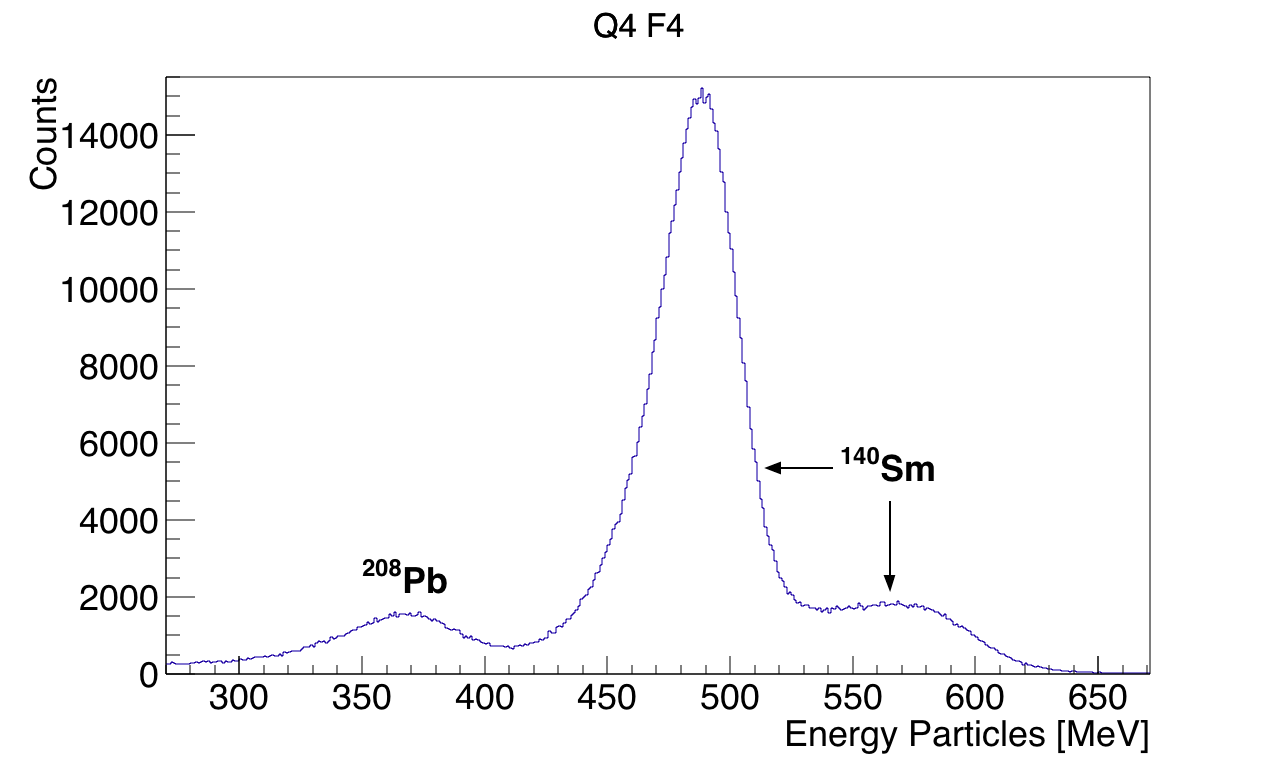
\includegraphics[width=\textwidth]{../Plots/plotting/TB_Q4_F4_cal.png}


\subsection{User calibration of the particle detector}\label{ssec:user_cal}

%In the present experiment there is only 2 data points to calibrate the CD, the peaks of \Sm\ and \Pb.
%However, the calibration for the CD is not expected to change significantly during a campaign of several experiments. 
%It is therefore possible to combine data from several experiments to make a common calibration file.
%On the positive side, there are many more data points in the calibration.
%The negative side is that the parameters might have changed slightly over time. 

To improve the calibration coefficients, it is possible to redo the calibration and apply energy peaks from the current experiment, i.e. perform an user calibration. 
This is an extensive task due to the large number of detector segments. 
The total amount of annular strips to calibrate on the front side of the CD is 64, since there is 4 quadrants with 16 rings. 
On the back side, there is effectively 48 radial strips, 4 quadrants with 12 strips.
To fully calibrate the CD, we need all the centroids of the peaks from both sides, 128 centroids (64 annular strips $\cdot$ 2 peaks/strip) on the front side and 1536 centroids (48 radial strips $\cdot$ 2 peaks/strip $\cdot$ 16 rings) on the back side. 
This gives a total of 1664 centroids to extract, which is not a task one would like to do manually.
However, it is possible to do a less precise calibration by only applying two peaks in each annular strip, and two peaks in each radial strip, making it in total 224 centroids to extract. 
Either way, the calibration coefficients of every ADC channel for the CD are obtained by performing a linear regression of the extracted centroids.

Calibrating the back strips of the CD is the same as the front.
However, the radial strips cover a large range of scattering angles (the whole radius of the CD). 
Because the particle energy depends strongly on the scattering angle, the spectra for the radial strips are washed out and show no clear energy (channel) peaks as displayed by \autoref{fig:th_b}.
For the energy calibration of the sectors on the back it is necessary to sort particle coincidence spectra between front rings and back sectors, i.e. spectra for each pixel of the detector.
Since these spectra are only needed for calibration, a separate code named \texttt{AQ4Sort} is used to produce them.
In addition to the \texttt{TreeBuilder} code, the \texttt{AQ4Sort} code is found in the Miniball GitHub repository \cite{MBCS}.
There exist no documentation or \textit{README} file explaining how to run the \texttt{AQ4Sort} subroutine. 
It can be operated in a similar way to the \texttt{TreeBuilder} code, but it does not take any command line flag options.
Compared to \texttt{TreeBuilder}, \texttt{AQ4Sort} sorts the histograms in a different way.
By using \texttt{AQ4Sort}, every single front strip and back strip combination, i.e. every pixel of the CD, can be viewed. 
Therefore, it is possible to gate on a peak in the annular (front) ring and align it with a peak in the corresponding radial (back) strip, thus calibrating the particle detector. 
For the radial strips, it is preferable to at least extract centroids for low, mid and high energies to cover the angular range of the strip. 
For example gating on ring 1, 8 and 16. 
%Calibrating the back strips of the CD is the same as the front, however because they cover a large range of angles in the $\theta$ direction (according to the LAB frame in \autoref{fig:scattering}), a gate on one of the front strips is needed to define an angle and thereby an energy. 
%For this purpose, the program \texttt{AQ4Sort} is used. 
%It operates on the same files as \texttt{TreeBuilder}, but with the purpose of making every combination of gates on front and back strips so that the front and back centroids for every "pixel" of the detector is available. 
%From \texttt{TreeBuilder}, only the front side calibration coefficients of the CD can be extracted. 
%For the back side, \texttt{AQ4Sort} has to be used.

As mentioned in \autoref{sec:detector_cal}, minimum two data points are required to obtain the calibration coefficients of \autoref{eq:offset} and \autoref{eq:gain}.
On the front side of the CD, there are effectively only two measuring points per angle interval. 
%If the contaminant in the spectra was known and if it only consists of one element, it could have been a third measuring point for a centroid in the calibration. 
On the back side of the CD there are two peaks per gated annular strip that can be fitted, so per back strip a maximum of 32 measuring points. 
By utilizing a built in ROOT fitting function, Gaussian or other, the centroids of the peaks for both Sm and Pb can be extracted. 
On the front side of the CD, \autoref{eq:offset} and \autoref{eq:gain} can be used to calculate the calibration coefficients:
\begin{align}\label{eq:GPandA}
	g_p &= \frac{E_{\text{Sm}} - E_{\text{Pb}}}{n_{\text{Sm}} - n_{\text{Pb}}} 
	&  
	a &= E_{\rho} - g_p \cdot n_{\rho}
\end{align}
where the $g_p$ is the gain for the particle, $a$ is the offset, $n$ is the channel number and $\rho$ can be either Sm or Pb.
For more than two centroids per strip, as the back side of the CD have, a linear regression method is used to find the best fit of the calibration coefficients.
The linear regression method is using least squares of a 1st degree polynomial \cite{Polyfit} to fit a line that re-produces the centroid points as best as possible, where the slope corresponds to the gain and the constant term corresponds to the offset.

An ambitious goal of the calibration of the current data set was to make a program that could automatically fit the centroid of the desired energy peaks by means of the ROOT framework. 
As will be explained in the current section, the task faced several difficulties, and in the end required a great deal of manual labor from the user.

In order to streamline the calibration process a bash script called \texttt{Q4S.sh} was written. 
\texttt{Q4S.sh} uses either \texttt{TreeBuilder} or \texttt{AQ4Sort} to sort large numbers of data files in one go.
The \textit{OnBeam.root}-files are loaded into \texttt{TreeBuilder} via \texttt{Q4S.sh} with the commands
%\begin{lstlisting}[language=sh]
%$ cd ~/GitHub/MasterThesis/Scripts/sorting 
%$ ./Q4S.sh Sm online TB
%... <showing output from script>
%\end{lstlisting}
%$ mv Sm_online-TreeBuilder-2019-06-24.root ../../Sorted_data/
%After the sorting, the file was moved to a folder of sorted data with the \textbf{mv} command, and the relative path was given to the \textit{setup\_Sm.txt} file used as input in the \texttt{ParticlePlot.cpp} script. 
%This script was made to extract different histograms from the \textit{.root}-file generated by either \texttt{TreeBuilder} or \texttt{AQ4Sort}.
%The script has to be loaded into the ROOT framework to work, because it was built to utilize the power of the framework.
%Histograms extracted from this step go through some formatting changes, to make them more presentable.
%To run the \texttt{ParticlePlot.cpp} in interaction with ROOT, the following commands are used
%\begin{lstlisting}[language=sh]
%$ cd ~/GitHub/MasterThesis/Scripts/plotting 
%$ root
%root [0] .L ParticlePlot.cpp++
%root [1] plot_front_back_energy("setup_Sm.txt", "online")
%... <showing output from script>
%\end{lstlisting}
%An example of how to use \texttt{Q4S.sh} with \texttt{TreeBuilder} is shown below
\begin{lstlisting}[language=]
$ cd ~/GitHub/MasterThesis/Scripts/sorting 
$ ./Q4S.sh Sm user TB
--- TreeBuilder ---
input file(s):
... <shows a list of all input files>
output file: Sm_user-TreeBuilder-2019-06-20.root
calibration file: ../../Miniball-config/IS558-user.cal
WeightPR: 0.75
Particle distribution:
 Q0 fired: 12243817
 Q1 fired: 12277727
 Q2 fired: 11479362
 Q3 fired: 10936096
Finished.
\end{lstlisting}
%$ mv Sm_user-TreeBuilder-2019-06-20.root ../../Sorted_data/
In the output, there is a line reading WeightPR: 0.75. 
This parameter is needed when calibrating the \ga\ detectors explained in \autoref{ssec:gamma}. 
%A similar example of how to use \texttt{Q4S.sh} with \texttt{AQ4Sort} is shown below
%\begin{lstlisting}[language=]
%$ ./Q4S.sh Sm user Q4
%Info: No flag option for 'AQ4Sort'. Ignoring optional flag.
%--- AQ4Sort ---
%calibration file: ../../Miniball-config/IS558-user.cal
%input file(s):
%... <shows a list of all input files>
%output file: Sm_user-AQ4Sort-2019-06-24.root
%$ mv Sm_user-AQ4Sort-2019-06-24.root ../../Sorted_data/
%\end{lstlisting}

\autoref{fig:cal_FC} shows a flowchart of the programs, scripts and files used in the user calibration. 
The strategy to perform the calibration of the CD is to combine the simulated data from \texttt{kinsim3.cc} and the experimental data sorted with \texttt{AQ4Sort} in order to obtain the calibration coefficients.
\texttt{kinsim3} delivers the energy centroids of \autoref{eq:GPandA}, while \texttt{AQ4Sort} delivers the channel numbers.
These two data sets are then analyzed using ROOT through different functions in the \texttt{ParticlePlot.cpp} script. 
Information about the range of the peaks and guesses of the centroids of Pb and Sm is written into input files applied by \texttt{ParticleFit.cpp}. 
Here, the automatic fitting collects the centroids of both data sets and write them into output files which is used as input by \texttt{particle-calibration.py}. 
This Python script plots the centroids and uses the linear regression method to extract the gain and offset values.
The values are written out into separate output files which are used as input in \texttt{ADC\_generator.py}. 
This Python script writes the calibration coefficients to the terminal, and from there they are copied and pasted into the calibration file \textit{IS5558-user.cal}.
The calibration coefficients given to the calibration file follow the naming convention of \texttt{TreeBuilder} in \autoref{tab:TBvsAQ4}. 
This new calibration file is then used to sort the data once more with \texttt{Q4S.sh}, but using \texttt{TreeBuilder} this time.
To visualize plots after a new calibration, either ROOT or \texttt{ParticlePlot.cpp} is used. 
The gray boxes in \autoref{fig:cal_FC} related to the \ga-calibration are discussed in \autoref{ssec:gamma}.

\begin{figure}[ht]
	\centering
	%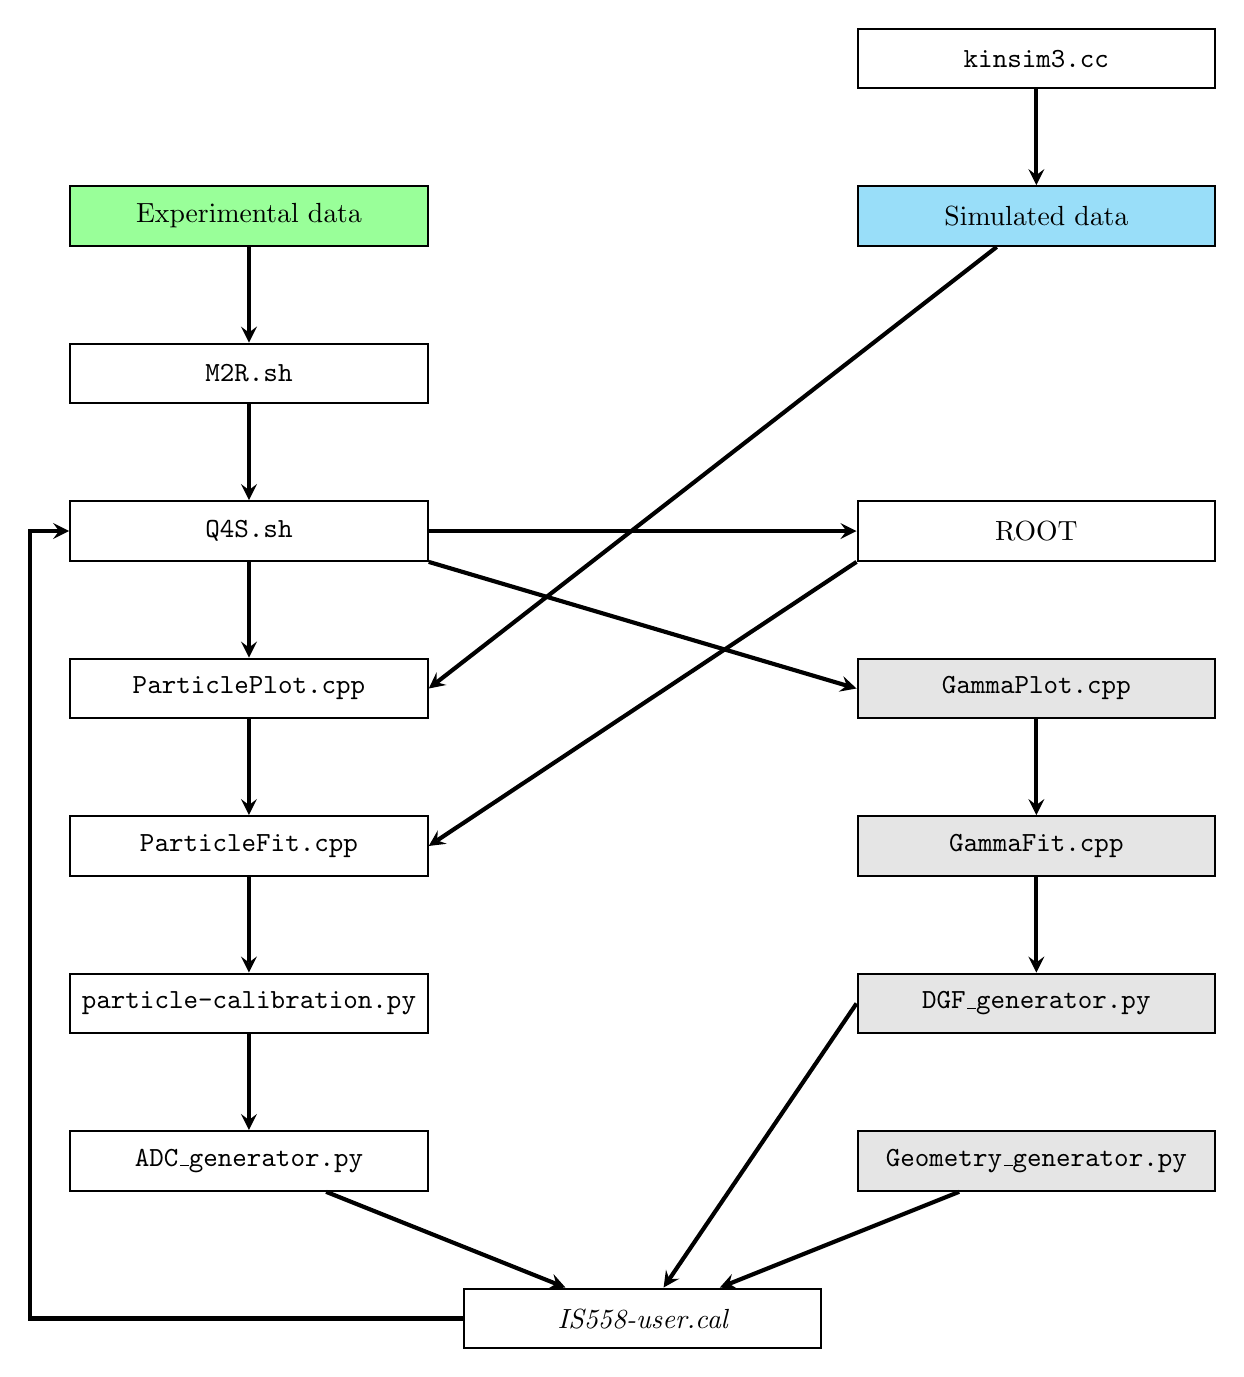
\begin{tikzpicture}[
    box/.style = { draw,minimum width=+30ex,minimum height=+5ex,thick },
    arrowstyle/.style = { ->,>=stealth,line width=1.5pt }
    ]
    % Definitions
    \coordinate (ks3)  at ( 5, 2 );
    \coordinate (sim)  at ( 5, 0 );
    \coordinate (exp)  at (-5, 0 );
    \coordinate (M2R)  at (-5,-2 );
    \coordinate (Q4S)  at (-5,-4 );
    \coordinate (Pplt) at (-5,-6 );
    \coordinate (Pfit) at (-5,-8 );
    \coordinate (pcal) at (-5,-10);
    \coordinate (Pgen) at (-5,-12);
    \coordinate (ROOT) at ( 5,-4 );
    \coordinate (Gplt) at ( 5,-6 );
    \coordinate (Gfit) at ( 5,-8 );
    \coordinate (Dgen) at ( 5,-10);
    \coordinate (Ggen) at ( 5,-12);
    \coordinate (calf) at ( 0,-14);
    % Nodes
    \node(K)  at (ks3)  [box]               {$\texttt{kinsim3.cc}$};
    \node(S)  at (sim)  [box,fill=cyan!40]  {Simulated data};
    \node(E)  at (exp)  [box,fill=green!40] {Experimental data};
    \node(M)  at (M2R)  [box]               {$\texttt{M2R.sh}$};
    \node(A)  at (Q4S)  [box]               {$\texttt{Q4S.sh}$};
    \node(RT) at (ROOT) [box]               {ROOT};
    \node(PP) at (Pplt) [box]               {$\texttt{ParticlePlot.cpp}$};
    \node(PF) at (Pfit) [box]               {$\texttt{ParticleFit.cpp}$};
    \node(pc) at (pcal) [box]               {$\texttt{particle-calibration.py}$};
    \node(ag) at (Pgen) [box]               {$\texttt{ADC\_generator.py}$};
    \node(GP) at (Gplt) [box,fill=black!10] {$\texttt{GammaPlot.cpp}$};
    \node(GF) at (Gfit) [box,fill=black!10] {$\texttt{GammaFit.cpp}$};
    \node(dg) at (Dgen) [box,fill=black!10] {$\texttt{DGF\_generator.py}$};
    \node(gg) at (Ggen) [box,fill=black!10] {$\texttt{Geometry\_generator.py}$};
    \node(cf) at (calf) [box]               {$\textit{IS558-user.cal}$};
    % Arrows
    \draw[arrowstyle] (K)             -- (S);
    \draw[arrowstyle] (E)             -- (M);
    \draw[arrowstyle] (M)             -- (A);
    \draw[arrowstyle] (S)             -- (PP.east);
    \draw[arrowstyle] (A)             -- (PP);
    \draw[arrowstyle] (A.east)        -- (RT.west);
    \draw[arrowstyle] (A.south east)  -- (GP.west);
    \draw[arrowstyle] (RT.south west) -- (PF.east);
    \draw[arrowstyle] (PP)            -- (PF);
    \draw[arrowstyle] (PF)            -- (pc);
    \draw[arrowstyle] (pc)            -- (ag);
    \draw[arrowstyle] (ag)            -- (cf);
    \draw[arrowstyle] (GP)            -- (GF);
    \draw[arrowstyle] (GF)            -- (dg);
    \draw[arrowstyle] (dg.west)       -- (cf);
    \draw[arrowstyle] (gg)            -- (cf);
    \draw[arrowstyle] (cf.west)       |- node[] {} ++(-5.5,0) |- (A.west);
\end{tikzpicture}
	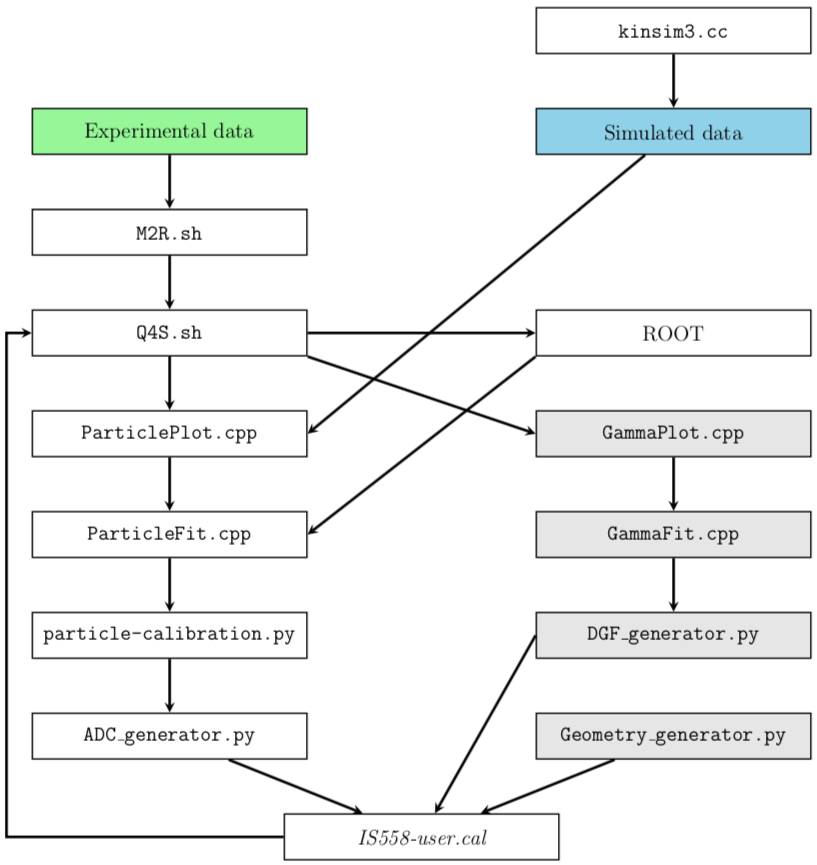
\includegraphics[width=0.8\textwidth]{Images/Flowchart.png}
	\caption{Flowchart of the programs, scripts and files applied in the user calibration. The relative paths of these programs and scripts are shown in \autoref{tab:paths}.}
	\label{fig:cal_FC}
\end{figure}

Several issues arose as the method of the automatic fitting was developed. 
The biggest complication was discovered when the method was tested on the radial strips of the CD.

In essence, the discrepancy between peak shapes are too large to calibrate the radial strips with a simple script.
% given a channel range for all 12 back strips. 
The fitting function can behave very strange given a too small or too big range.
Another problem is the complex shape of the peaks. 
\autoref{fig:CD_cal_easy} displays a strip that the automatic fitting handles well, while \autoref{fig:CD_cal_difficult} shows an example of a strip that is challenging to fit.
In \autoref{fig:CD_cal_easy}, it is fairly easy to determine the centroids of the particle peaks.
The shape of the \Pb\ peak in \autoref{fig:CD_cal_difficult} is very irregular and it is difficult to determine the centroid of the peak because of the overlapping contaminant at lower energies.
%In some spectra it was very difficult to determine the centroid of the Pb peaks especially at low energy, as shown in \autoref{fig:CD_cal_difficult}. 
In most cases the peak shapes are not Gaussian. 
%Looking at the energy vs. channel plots, we clearly saw that a Gaussian fit of the energy peaks did not describe the data.
A ROOT built in function of a 4th degree polynomial was tested to fit the complex peak shapes. 
The predefined ROOT function 
\begin{equation}
	f(x) = p_0 + p_1 \cdot x + p_2 \cdot x^2 + p_3 \cdot x^3 + p_4 \cdot x^4
\end{equation}
fits the values of the parameters automatically, given a initial guess by the user. 
Unfortunately, the 4th degree polynomial did not describe the peak shapes well either.
To implement a proper automatic fitting program, one would have to find a function with a negatively-skewed distribution, where most of the data values are concentrated on the right side of the distribution graph. 

\begin{figure}[ht]
	\centering
	\begin{subfigure}[t]{0.49\textwidth}
		\centering
		% ParticlePlot.cpp
		% get_single_plot("setup_Sm.txt", "tb", "f", 0, 4, 9, 1, 300, 2400, 1080)
		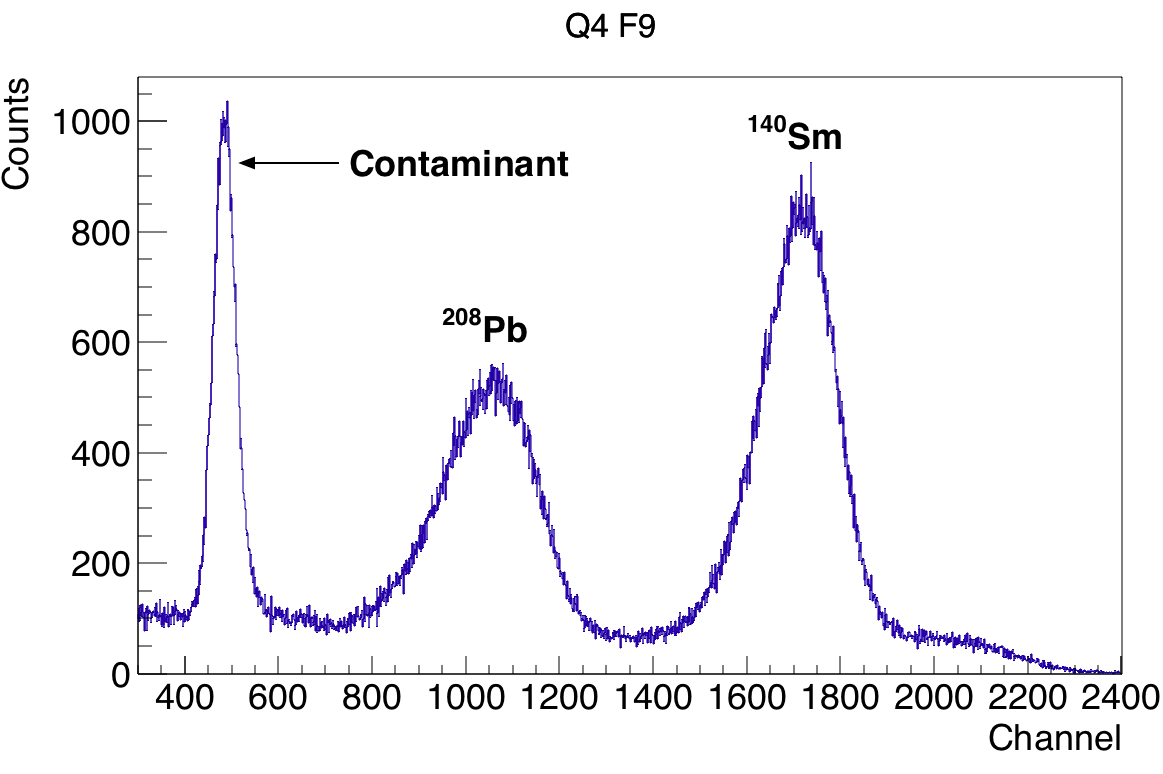
\includegraphics[width=\textwidth]{../Plots/plotting/TB_Q4_F9.png}
		\caption{}
		\label{fig:CD_cal_easy}
	\end{subfigure}
	\hfill
	\begin{subfigure}[t]{0.49\textwidth}
		\centering
		% ParticlePlot.cpp
		% get_single_plot("setup_Sm.txt", "q4", "b", 0, 1, 16, 12, 200, 1400, 330)
		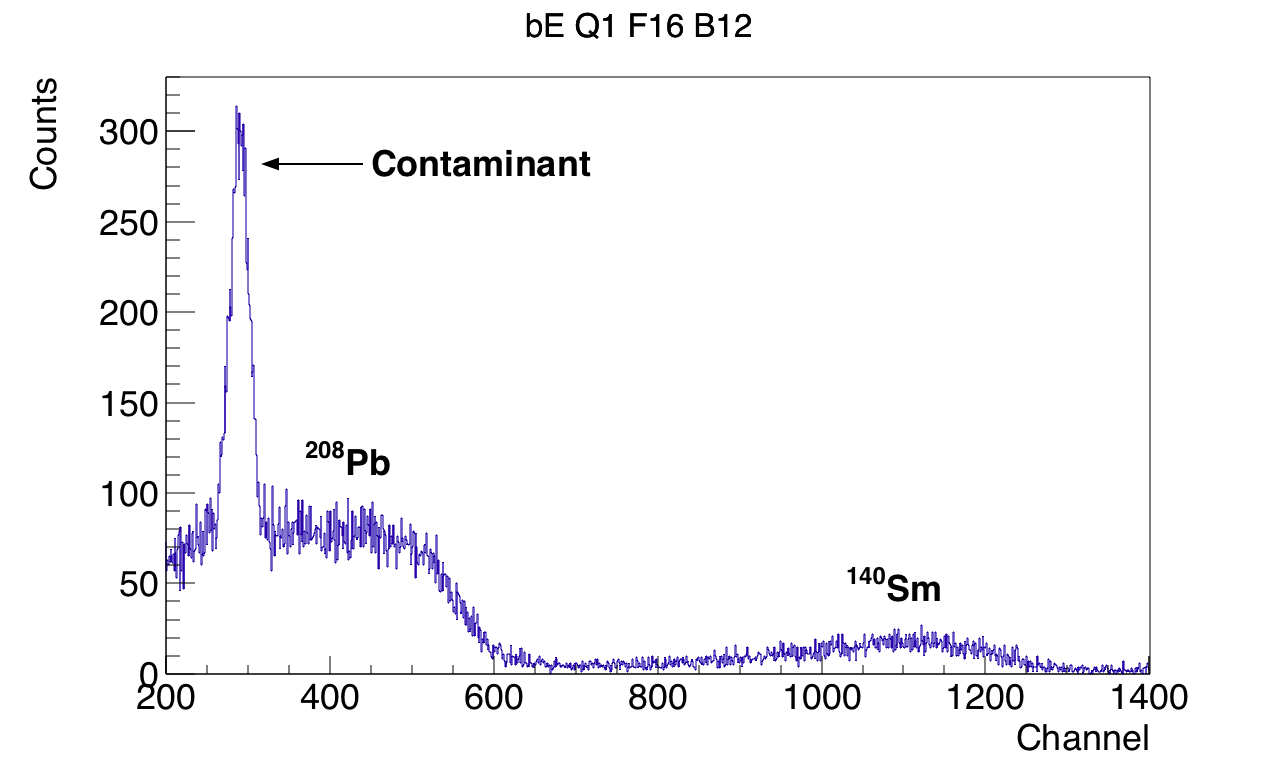
\includegraphics[width=\textwidth]{../Plots/plotting/bE_Q1_f16_b12.png}
		\caption{}
		\label{fig:CD_cal_difficult}
	\end{subfigure}
	\caption{\textbf{(a)} Front strip number 9 in quadrant 4. 
	\textbf{(b)} Back strip 12, gated on ring 16 (outermost ring) in quadrant 1. 
	See text for more information.}
	\label{fig:cal_ED}
\end{figure}

In logarithmic (log) $y$-scale, the data appears to be more Gaussian distributed, while the contrary is not the case in the linear y-scale. 
The automatic fitting worked better when a log y-scale was applied.
Unfortunately, as it turned out, the precision of the fit performed in log y-scale was not satisfactory.
One should be careful to inspect the quality of the fit on a linear scale, as it is more difficult to see deviations on a logarithmic scale. 

On lower energies, there are problems to properly extract the centroids.
To overcome this challenge, additional data obtained during experiment IS553 conducted immediately before the present experiment was applied in the detector calibration.
Unfortunately, the attempt including the data from experiment IS553 to improve the calibration was unsuccessful.
The quality of the data can be estimated by looking at how well the data lie on the diagonal line when plotting front against back energy.
%The experiment was IS553, $^{144}$Ba on $^{58}$Ni, and the reason for trying additional data was to try to get calibration for the lower energy spectra. 
%It may be that the energy loss or target thickness was wrong, or that the beam energy was different, or that the simulation didn't account for all the details of the stopping. 
%The only way to get a good calibration is to have as much data as possible and then kick out the bad data until there is a good fit. 
%What was clear at the moment was that the scatter between the data points from the different reactions was too large to simply average out with a straight line fit. 
%It is important to select data that agree.
%The fitting just didn't seem reliable.
%It gave a steeper slope than the online calibration.
%By looking at the front vs. back energy plots, the diagonal lines were almost disappearing in the middle, and they were a lot broader than the online calibration. 
%One big problem of not using the IS553 data, was that it was not possible to get any good calibration coefficients for front ring 16 and maybe also ring 15 (the two outermost rings).
%But this problem was also found in the IS553 data, even though the beam energy was less than the present experiment. 
When energy peaks from IS553 was included in the user calibration of the current experiment, the calibration appeared to look worse. 
Firstly, the diagonal line in the front vs. back energy spectra was not as defined as the online calibration in \autoref{fig:CD_cal_online}.
Secondly, the off-diagonal events seemed to increase, implying that there was an increase in the mismatch of front and back events. 
%The latter could be due to the visualization coming from the $z$-scale, since there are a different number of events in the quadrants. 
%It would have been nice with some low-energy points as well as high-energy points in order to do the calibration. 

%In principle it is possible to get a linear calibration for the current experiment from the data set alone. 
%The data needs to be compared with the simulated spectra. 
%A large number of peaks must be fitted, which requires automated routines.
%For certain angles, the peaks are very difficult to fit because of peak shapes, overlapping peaks, etc. 
%A possible solution is to combine the data with another data set where the additional peaks for the angles where it is difficult to fit the Pb in the data. 
%The problem is that the other data set needs to be compared with another simulation, and both changing physical conditions during the two experiments and systematic uncertainties related to two separate simulations make it difficult to extract a consistent calibration. 
%The approach of combining two data sets resulted in a worse calibration compared to the online calibration. 
%The quality of the data can be estimated by looking at how well the data lie on the diagonal line when plotting front against back energy.
%The approach with the cocktail beam has advantages, all peaks obtained under the same conditions using a thin target, so the peaks are more narrow and easier to fit. 

%To summarize, there was a dedicated online calibration run a few months before the experiment. 
%Since conditions change over time, the calibration had to be checked if it was still valid. 
%A better calibration was attempted with the experimental data, but it turned out to be difficult.
%Additional data, taken just the week before, was tried combining with the present experimental data, but this was unsuccessful. 
%Although it is possible to get a linear calibration for the current experiment from the data set alone, it is a difficult task, and the results were not as good as the online calibration. 
%The online detector calibration was in this case very stable.

%In principle it is possible to get a linear calibration for the current experiment from the data set alone. 
Given the numerous complications of the log scale, the shape of the peaks and the range of the fit, the automatic fitting procedure was discarded altogether. 
Although plentiful of time was used to develop scripts for the auto-fitting method, we decided to apply the online calibration in the end.
As we will see in \autoref{sec:BDS}, the main issue of the online calibration was in fact the calibration coefficients of the innermost ring.
What will later be described as the user calibration file is essentially the online calibration file without the innermost ring.

\begin{figure}[htb]
	\centering
	\begin{subfigure}[t]{0.49\textwidth}
		\centering
		% ParticlePlot.cpp
		% plot_single_front_back_energy("setup_Sm.txt", 1, "online")
		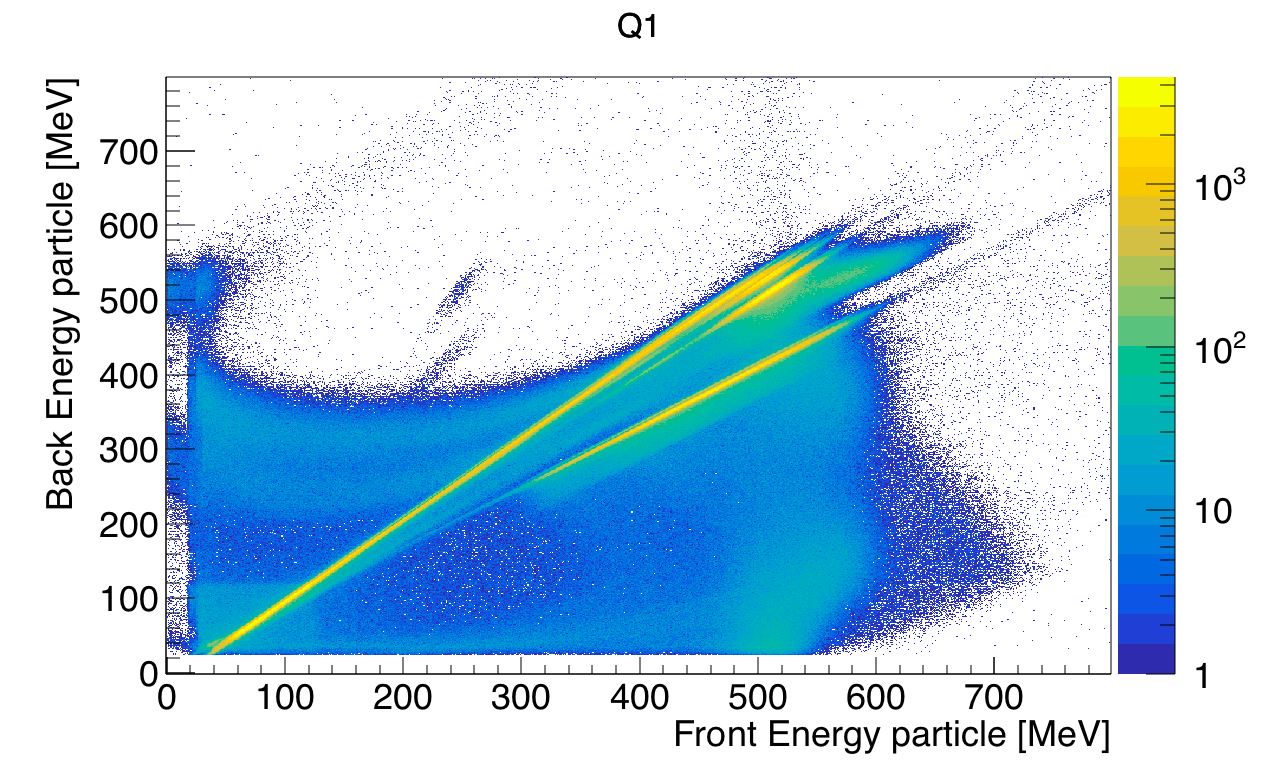
\includegraphics[width=\textwidth]{../Plots/plotting/E_f_b_Q1-online.png}
		\caption{}
		\label{fig:CD_cal_online}
	\end{subfigure}
	\hfill
	\begin{subfigure}[t]{0.49\textwidth}
		\centering
		% ParticlePlot.cpp
		% plot_single_front_back_energy("setup_Sm.txt", 4, "user")
		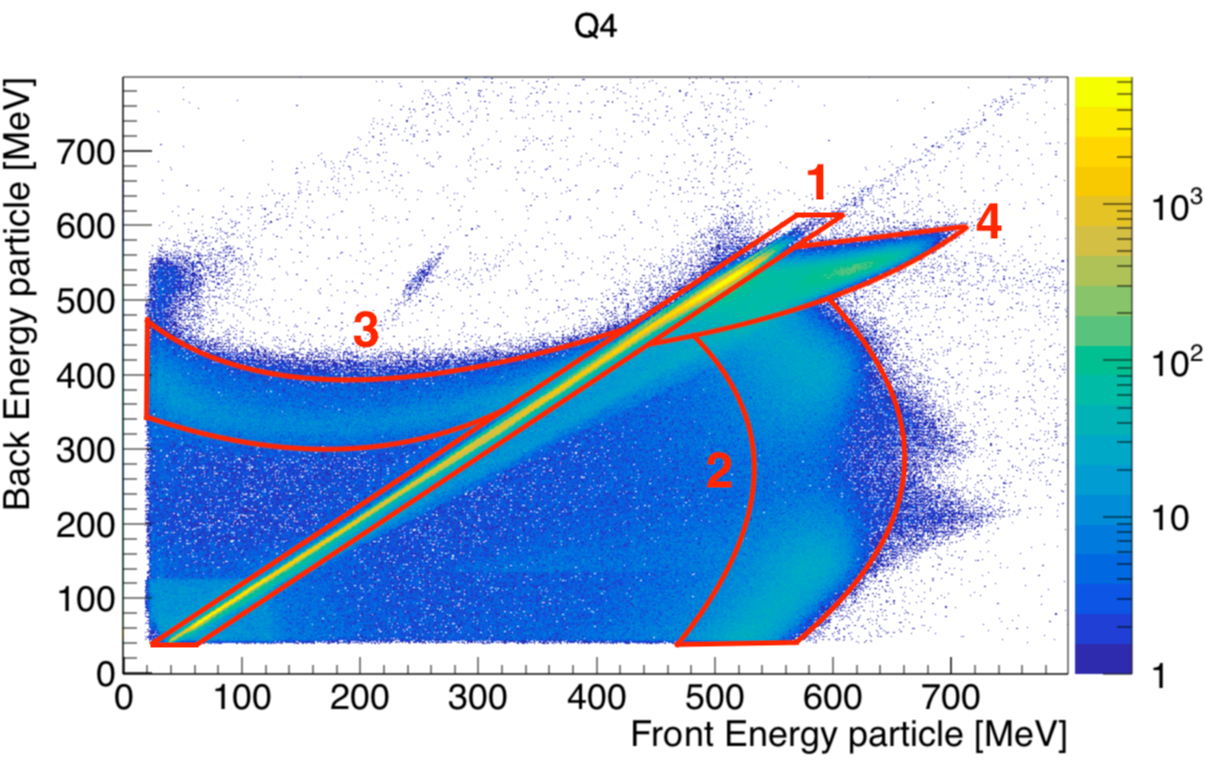
\includegraphics[width=\textwidth]{../Plots/plotting/E_f_b_Q4-user-drawing.png}
		\caption{}
		\label{fig:EFBQ4}
	\end{subfigure}
	%
	\begin{subfigure}[t]{0.49\textwidth}
		\centering
		% ParticlePlot.cpp
		% single_CD_energy("setup_Sm.txt", "b", 1)
		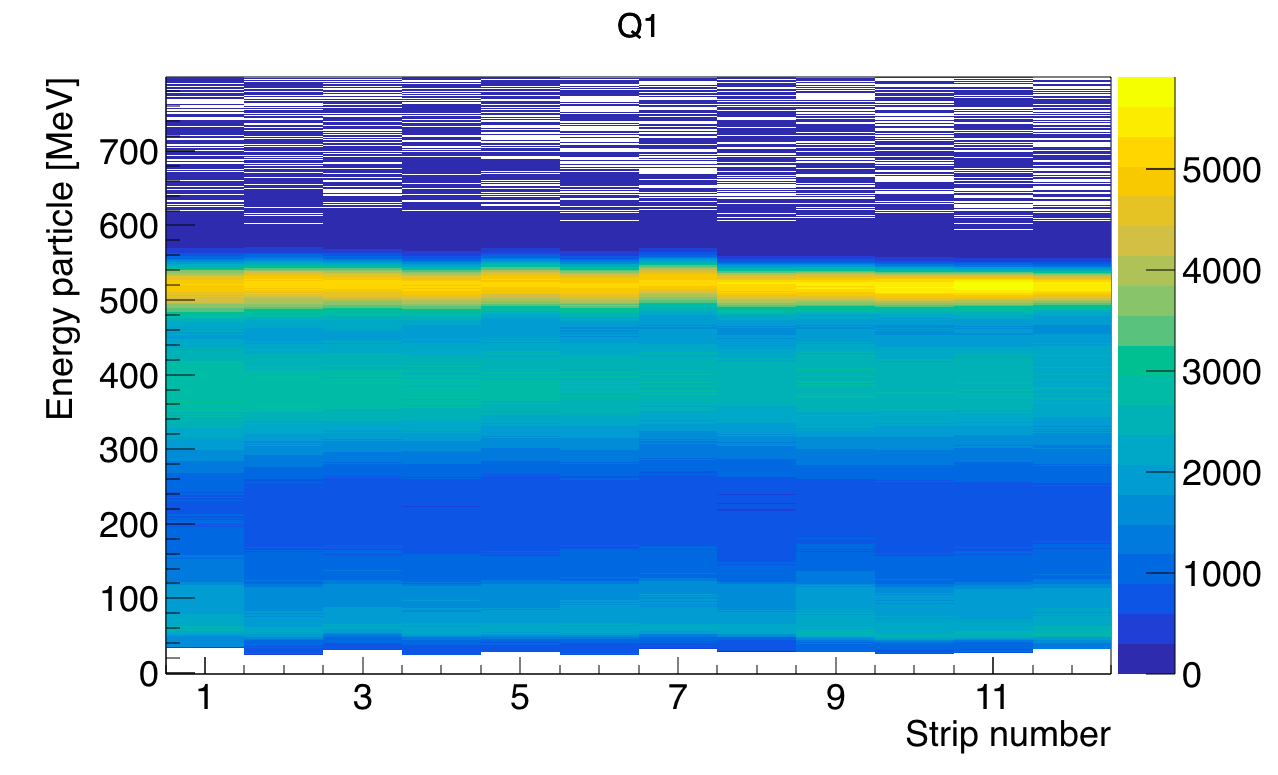
\includegraphics[width=\textwidth]{../Plots/plotting/E_vs_b-strip_Q1.png}
		\caption{}
		\label{fig:CD_cal_back}
	\end{subfigure}
	\caption{Back energy vs. front energy for one quadrant of the CD in \textbf{(a+b)}. 
	\textbf{(a)} Quadrant 1 using the online calibration.
	\textbf{(b)} Quadrant 4 using the user calibration. The marked regions are explained in \autoref{ssec:DPS} and are similar to figures 39 and 40 in \cite{Rosiak}.
	\textbf{(c)} Quadrant 1 of the back side of the CD using the user calibration. A number of the radial strips have incorrect gains, as they don't lie on the straight line.
	See text for more information.}
	\label{fig:FBE}
\end{figure}

%\begin{figure}[ht]
%	\centering
%	\begin{subfigure}{\textwidth}
%		\centering
%		% ParticlePlot.cpp
%		% plot_front_back_energy("setup_Sm.txt", "online")
%		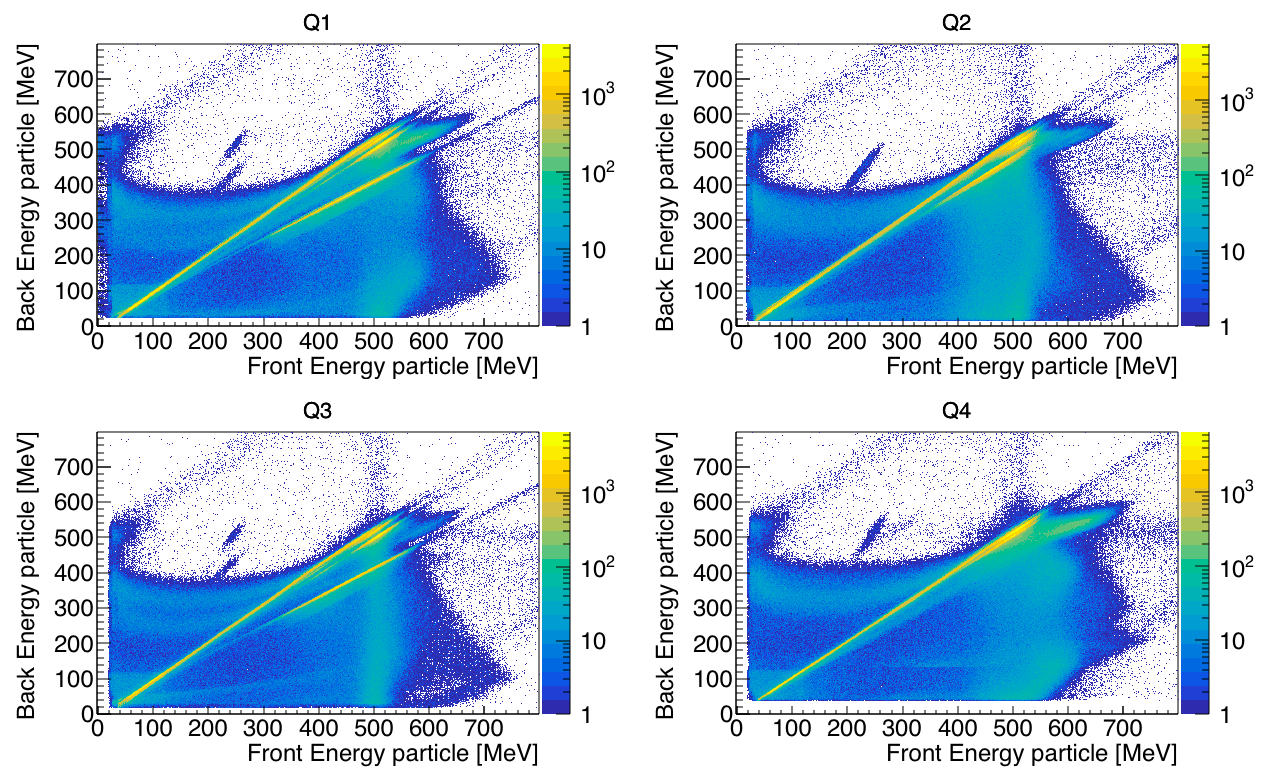
\includegraphics[width=\textwidth]{../Plots/plotting/E_f_b_Q1-4-online.png}
%		\caption{Online calibration for the CD showing the four quadrants. It generally looks quite good, but there is a number of the radial strips (back side) that have the wrong gains.}
%		\label{fig:CD_cal_online}
%	\end{subfigure}
%	\begin{subfigure}{\textwidth}
%		\centering
%		% ParticlePlot.cpp
%		% plot_front_back_energy("setup_Sm.txt", "user")
%		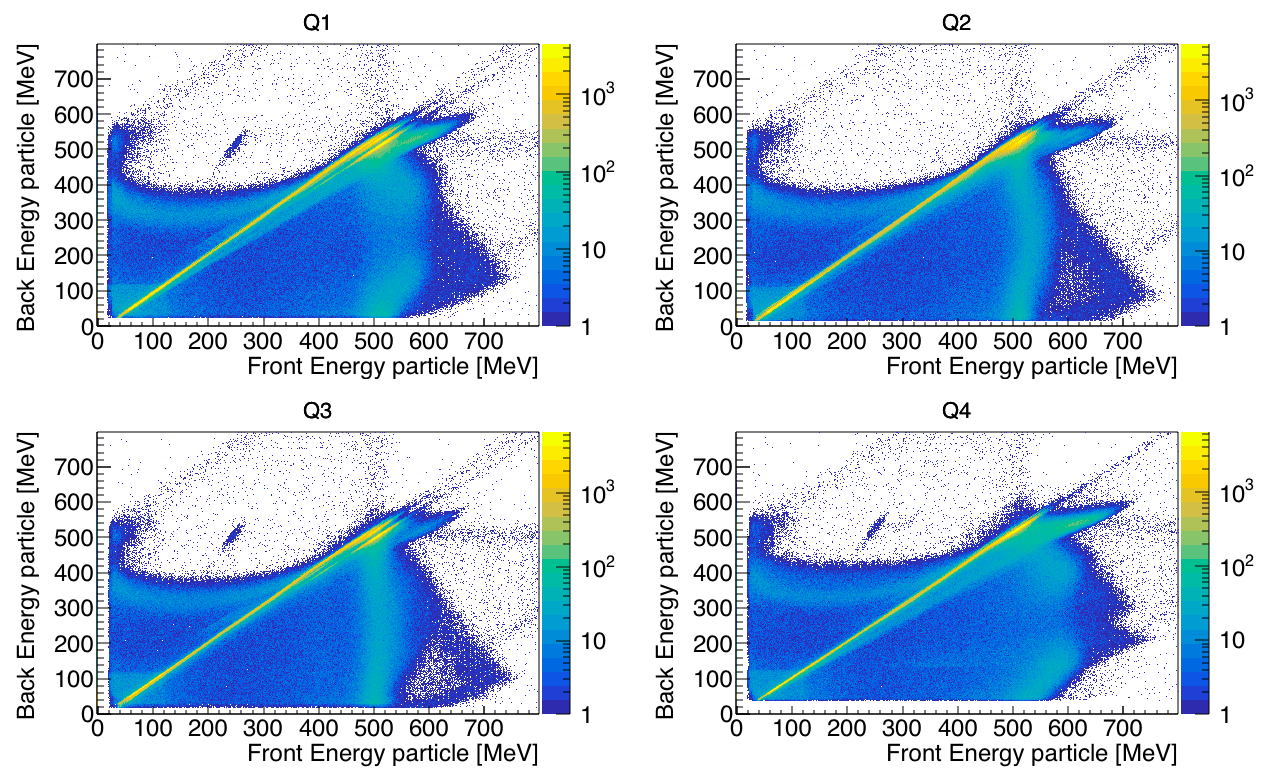
\includegraphics[width=\textwidth]{../Plots/plotting/E_f_b_Q1-4-user.png}
%		\caption{User calibration for the CD showing the four quadrants. This is actually the online calibration without the innermost ring, which was broken.}
%		\label{fig:cal_FB}
%	\end{subfigure}
%	\caption{Back energy vs. front energy for each quadrant of the CD.}
%	\label{fig:cal_OU}
%\end{figure}
% -------------------------------------------------------------------------------------------------
%\begin{figure}[ht]
%	\centering
%	\begin{subfigure}{\textwidth}
%		\centering
%		% ParticlePlot.cpp		
%		% CD_energy("setup_Sm.txt", "f")
%		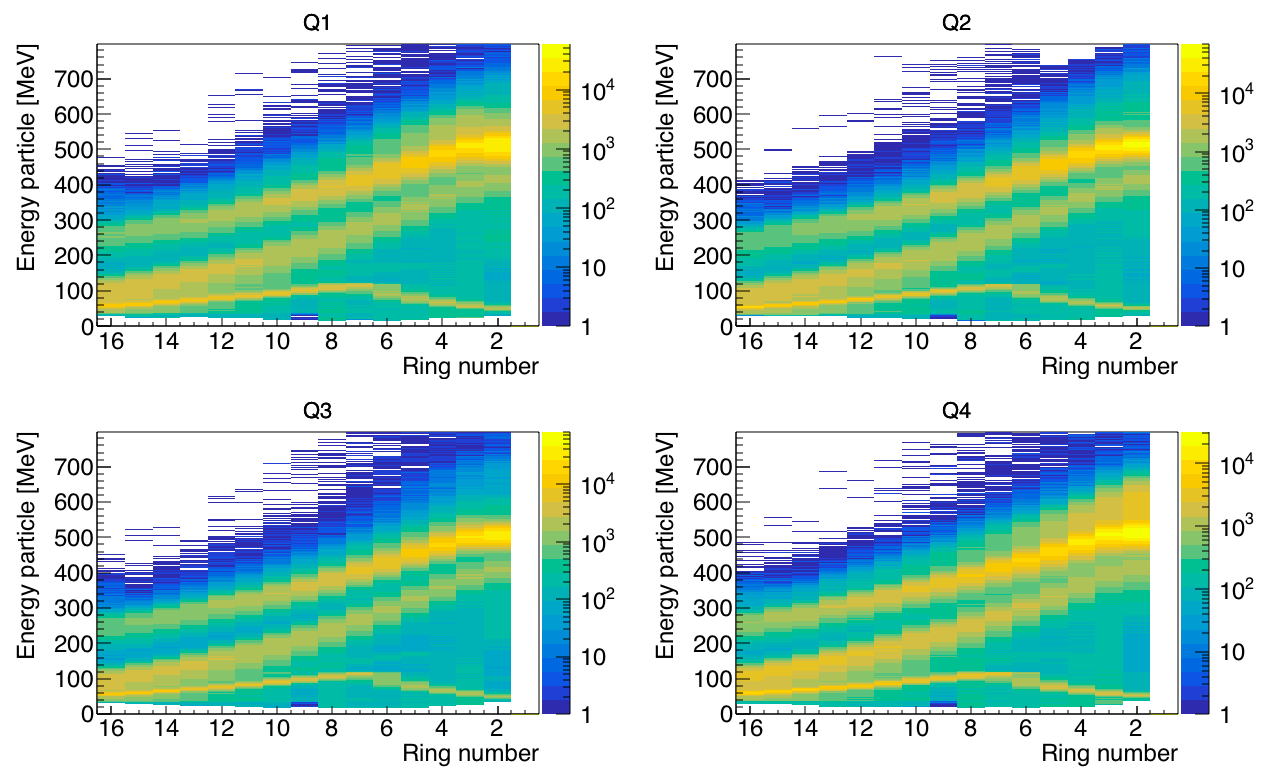
\includegraphics[width=\textwidth]{../Plots/plotting/E_vs_f-strip_all_Q.png}
%		\caption{CD front. Ring number 16 is the outermost ring and ring number 1 is the innermost ring.}
%		\label{fig:cal_CD_front}
%	\end{subfigure}
%	%%
%	%%
%	\caption{Energy vs. strip number for each quadrant of the CD.}
%	\label{fig:cal_CD}
%\end{figure}


\subsection{The double peak structure}\label{ssec:DPS}
In several strips of quadrant 1 and 4, there we observe a double-peak structure of \Sm\ similar to the peaks displayed in \autoref{fig:th_f}. 
To explain this we have to look at the two-dimensional (2D) spectrum in \autoref{fig:EFBQ4}, which can be divided into four parts \cite{Rosiak}:
\begin{itemize}
	\item Region 1: The measured energy at the front and back side of the CD are equal, which indicates that they are linearly correlated.
	\item Region 2: In these events the detected energy is lower at the back side, while at the front side the energy is artificially increased. 
	One explanation of this is if the energy is detected in one strip on the front side, but is shared between two neighboring strips on the back side.
	The reduced energy on the back side only occurs when the impact position is close to or inside the dead layer between two strips. 
	The current from the two neighboring strips can possibly induce an artificially higher energy to the front side of the CD. 
	A similar phenomenon has been observed in segmented HPGe detectors discussed in detail in \cite{Bruyneel2006a, Bruyneel2006b, Bruyneel, Descovich2005, Abt2017}.	
	Another explanation is that there are some charge trapping and charge recombination of the particle-hole pairs. 
	This causes a Pulse-Height Defect (PHD) in the detector signal, which is discussed in detail in \cite{Miller1962, Wilkins1971}.
	
	The second Sm-peak at higher energies in \autoref{fig:th_f} comes from the projection of the 2D spectrum from \autoref{fig:EFBQ4} onto the x-axis.
	\item Region 3: This area has a similar, but different pattern to region 2. 
	The detected energy is lower at the front side, while it is higher at the back side of the CD. 
	Here, the reduced energy on the front side is likely to originate from charge sharing between neighboring annular strips if the incoming particle hits close to or inside the dead layer. 
	 On the back side, the strips are coupled to a positive voltage which protects against the induction of an artificially higher energy by the front side charge sharing. 
	These phenomena are discussed in detail in \cite{Grassi2014, Kramberger2002}.
	\item Region 4: This structure originates from the same effects as region 2.
	These events occur because of the paired up radial strips on the back side of the CD.  
	Because of the connection of two neighboring strips, the charge is split among them and added up to the total charge.
\end{itemize}

\begin{figure}[htb]
	\centering
	\begin{subfigure}[t]{0.49\textwidth}
		\centering
		% GammaPlot.cpp
		% check_single_threshold("setup_Sm.txt", "f", 4, 2, 3300, 8000)
		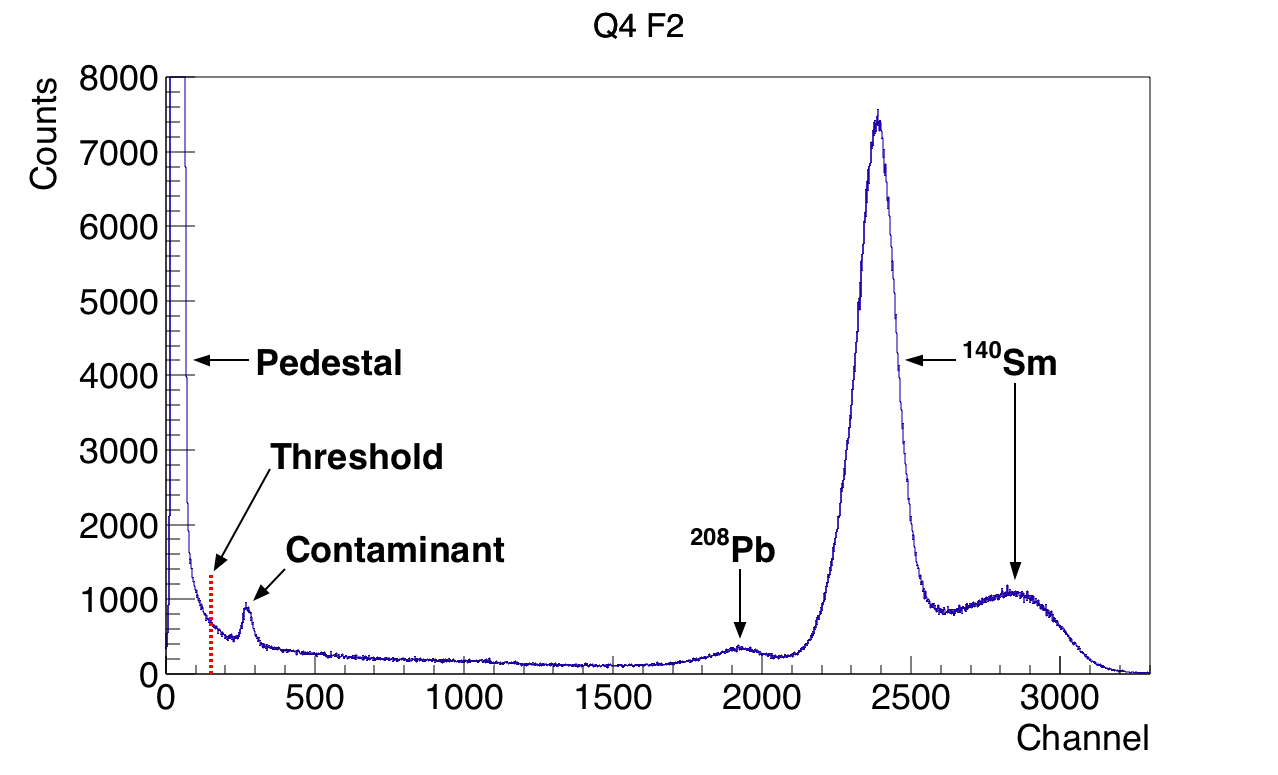
\includegraphics[width=\textwidth]{../Plots/plotting/Threshold_Q4_f2.png}
		\caption{}
		\label{fig:th_f}
	\end{subfigure}
	\hfill 
	\begin{subfigure}[t]{0.49\textwidth}
		\centering
		% GammaPlot.cpp
		% check_single_threshold("setup_Sm.txt", "b", 4, 6, 2700, 2000)
    		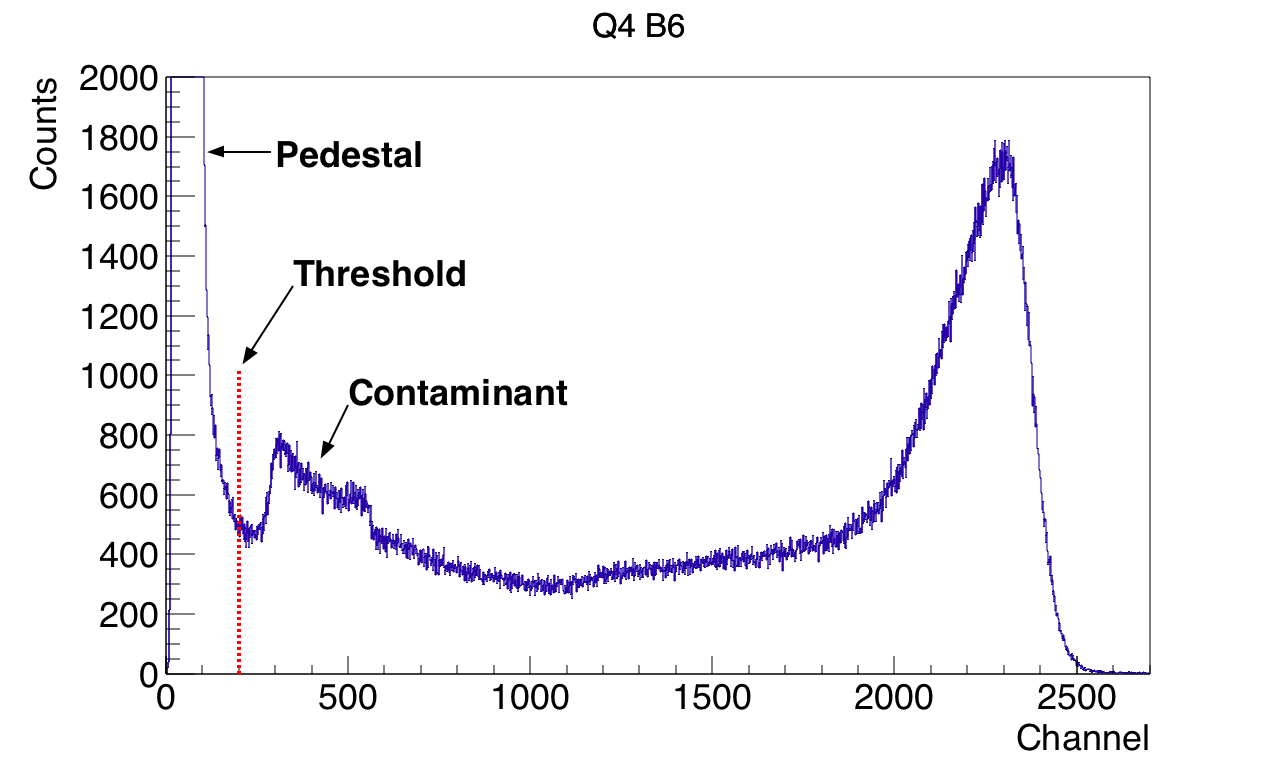
\includegraphics[width=\textwidth]{../Plots/plotting/Threshold_Q4_b6.png}
		\caption{}
		\label{fig:th_b}
	\end{subfigure}
	\caption{\textbf{(a)} Front strip number 2 in quadrant 4. 
	At higher energies, there is a double-peak structure of \Sm. 
	The second peak of \Sm\ can be explained by region 2 from \autoref{fig:EFBQ4}.
	\textbf{(b)} Back strip number 6 in quadrant 4.
	See text for more information.}
	\label{fig:threshold}
\end{figure}


\subsection{CD threshold}\label{ssec:threshold}
In the CD, the continuum of events at low energy comes from charge sharing between the strips.
\autoref{fig:threshold} shows the big peak of the charge sharing on the front and back side of the CD. 
This peak is called the "pedestal". 
For the very heavy ions, the total amount of charge deposited gets split between neighboring strips of the CD. 
There is a single common gate for each ADC, containing channels from one CD quadrant. 
Therefore, when there is an event in one strip of the CD, all channels are read out, but the channels without a real event read a non-zero energy.
These are the events in the pedestal.
\textsl{MiniballCoulexSort} perform a few tricks to try to recover the correct energy and position of the particles. 
The energy and position of the particles depends on counting the number of strips that fire.

A software threshold is applied to cut away the pedestal. 
For each ADC channel, the threshold can, and should be set. 
If no threshold is given in the calibration file, the default threshold is set to channel 100.
One should define the threshold for each ADC channel to be above the pedestal peak.
If the threshold is set too low, pedestal events are included in the sorting routine, potentially causing harmful issues.
If the threshold is too high, several charge-sharing events will be leading to false particle energy.
After a correct calibration and threshold is applied, the pedestal will be calibrated out of the physical energy range, meaning it is cut away in the spectra.

The goal is to not include the pedestal, and not to cut away too many continuum events.
%It is easier to set thresholds in linear scale than logarithmic, because in it is difficult to see where to correctly set the limit. 
\autoref{fig:th_f} and \autoref{fig:th_b} shows the software threshold set in the calibration file on the front and back side for one strip on each side.
To verify that the implemented threshold is correct, it is very useful to check the so-called "debug" histogram from \texttt{TreeBuilder} displayed in \autoref{fig:CD_debug} and the detected particle events in \autoref{fig:part_wcut}.
\autoref{fig:CD_debug} is a histogram of how many strips of the CD fired per particle.
It counts how many particles have lead to $x$ strips fired on the front side and $y$ strips fired on the back side. 
The table in \autoref{fig:CD_debug_table} explains the different debug IDs, i.e. lists the $x$-axis of \autoref{fig:CD_debug}. 
The goal of the threshold is to have a lot more counts in CD debug ID 0 compared to ID 3.
If we have too many debug ID = 3, then the threshold is too low. 
If we have a large continuum/background in \autoref{fig:part_wcut}, the thresholds are too high. 
This way, it is possible to test different values for the threshold and choose the best suited value.
The code yields debug ID 20 when no particle can be found, i.e. there is no energy registered in either the front or the back strips. 
This can only happen when the front energy is below the software threshold set by the user in the calibration file and the back energy is either in a broken strip, or below the software threshold. 
Charge sharing and noise events will in general also occur below the threshold.
Therefore, it is expected that debug ID 20 always have a significant number of counts.

\begin{figure}[htb]
	\centering
	\begin{subfigure}[b]{0.49\textwidth}
		\centering
		% ParticlePlot.cpp
		% check_cd_debug("setup_Sm.txt", "user")
		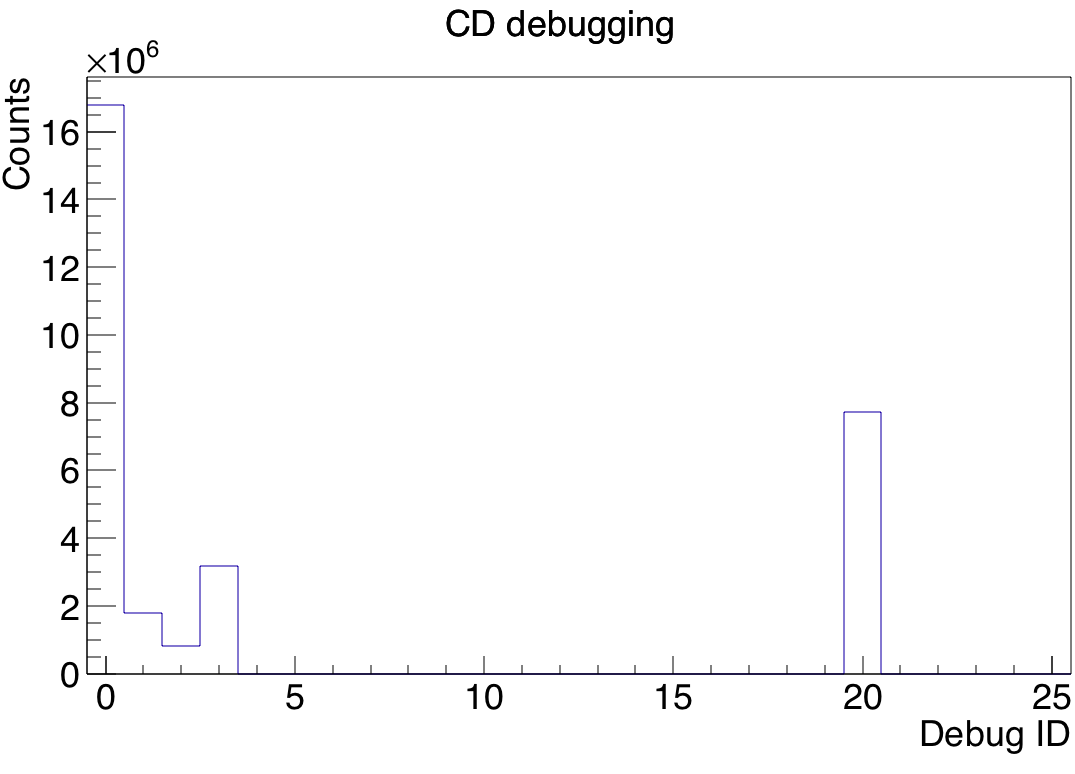
\includegraphics[width=\textwidth]{../Plots/plotting/cd_debug-user.png}
		\caption{}
		\label{fig:CD_debug}
	\end{subfigure}
	\hfill
	\begin{subfigure}[b]{0.49\textwidth}
		\centering
    		% Data for the CD angles table
\begin{tabular}{ccc}
\hline
             &  \multicolumn{2}{c}{Strips fired}       \\
CD debug ID  &  Front side &  Back side                \\
\hline
0            &     1       &     1                     \\
1            &     1       &     2                     \\
2            &     2       &     1                     \\
3            &  $>$1       &  $>$1                     \\
20           &  \multicolumn{2}{c}{No particle found}  \\
\hline
\end{tabular} \newline % newline lifts the table up one line
    		\caption{}
    		\label{fig:CD_debug_table}
	\end{subfigure}
	\caption{\textbf{(a)} A histogram of the CD debugging after a user threshold is set. The IDs on the $x$-axis are explained by the table in \textbf{(b)}. The IDs show the number of strips fired at the front and back side of the CD.}
	\label{fig:CD_debug_both}
\end{figure}



\subsection{Time calibration}\label{ssec:time_cal}
The purpose of the time calibration is to align the time spectra so that a time gate can be set. 
In this way it is possible to correlate particles and \ga-rays. 
\texttt{TreeBuilder} generates time offset histograms. 
The histograms displays the time difference between a detected particle and \ga\ with 25 ns ticks\footnote{In computers, the system time represents the passage of time. The system time is measured as counting the number of ticks since a starting date. Clock ticks generally refer to the system clock, which runs at a certain frequency, typically in Ghz. This means that there are billions of clock ticks (or cycles) per second. 25 ns ticks refers to one tick per 25 ns, meaning the ADC has a system clock or a CPU running at 40 Mhz.}.
Using the \texttt{ParticlePlot.cpp} script, the ADC time offset spectra can be extracted by the following commands
\begin{lstlisting}[language=sh]
$ cd ~/GitHub/MasterThesis/Scripts/plotting
$ root
root [0] .L ParticlePlot.cpp++
root [1] check_ADC_time_offsets("setup_Sm.txt")
\end{lstlisting}
%or they can be manually reached by
%\begin{lstlisting}[language=sh]
%$ cd ~/GitHub/MasterThesis/Sorted_data
%$ root Sm_user-TreeBuilder-2019-06-20.root
%root [1] new TBrowser()
%\end{lstlisting}
%In the browser, the histograms are named \textit{tdiff\_gp\_i}, where \textit{i} is a number between 0 and 3 implying quadrant 1 to 4. 
%They lie within the \textit{.root}-file without a folder. 
%\autoref{fig:ADC_dt} shows the time offsets for the CD. 
\autoref{fig:ADC_dt} displays the time offsets of all the quadrants of the CD.
Here, the time offset values are defined as the $x$-value of the maximum peak height.
The peak values, i.e. the time offsets, may change depending on the amount of data sorted.
Therefore, it is wise to double check the time offsets when more data is added to the \textit{.root}-file. 
After the peak values have been collected, they should be written into the calibration file together with the updated threshold. 
Then, the \texttt{Q4S.sh} script with \texttt{TreeBuilder} should be re-run to implement the changes in the calibration file. 
The time offsets utilized in this experiment was the following
\begin{lstlisting}[language=sh]
# ADC time offsets (ticks)
adc_0.TimeOffset:  0
adc_1.TimeOffset:  -2
adc_2.TimeOffset:  -3
adc_3.TimeOffset:  5
\end{lstlisting}

\begin{figure}[ht]
	\centering
	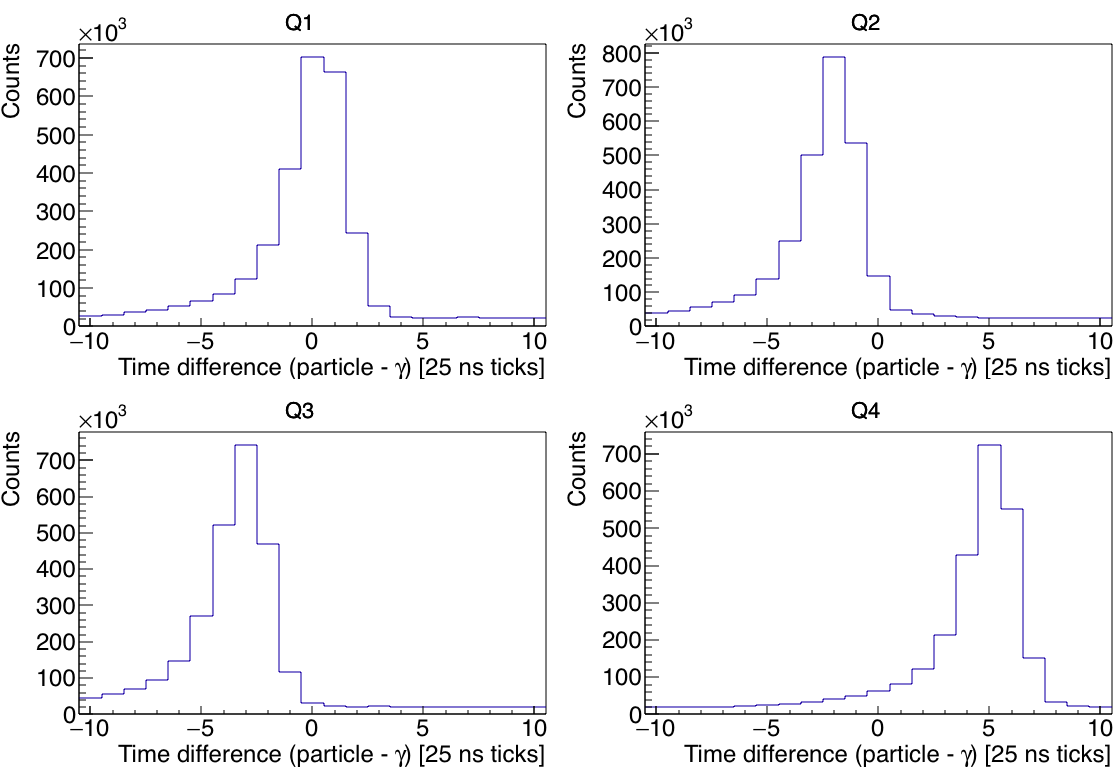
\includegraphics[width=\textwidth]{../Plots/plotting/tdiff_gp_0-3-user.png}
	\caption{ADC time offsets for the four quadrants of the CD. 
	See the text for more information.}
	\label{fig:ADC_dt}
\end{figure}

%\begin{figure}[ht]
%	\centering
%	\begin{subfigure}{\textwidth}
%		\centering
%		% ParticlePlot.cpp
%		% check_pedestal("setup_Sm.txt", "f", 2, 4, 60)
%		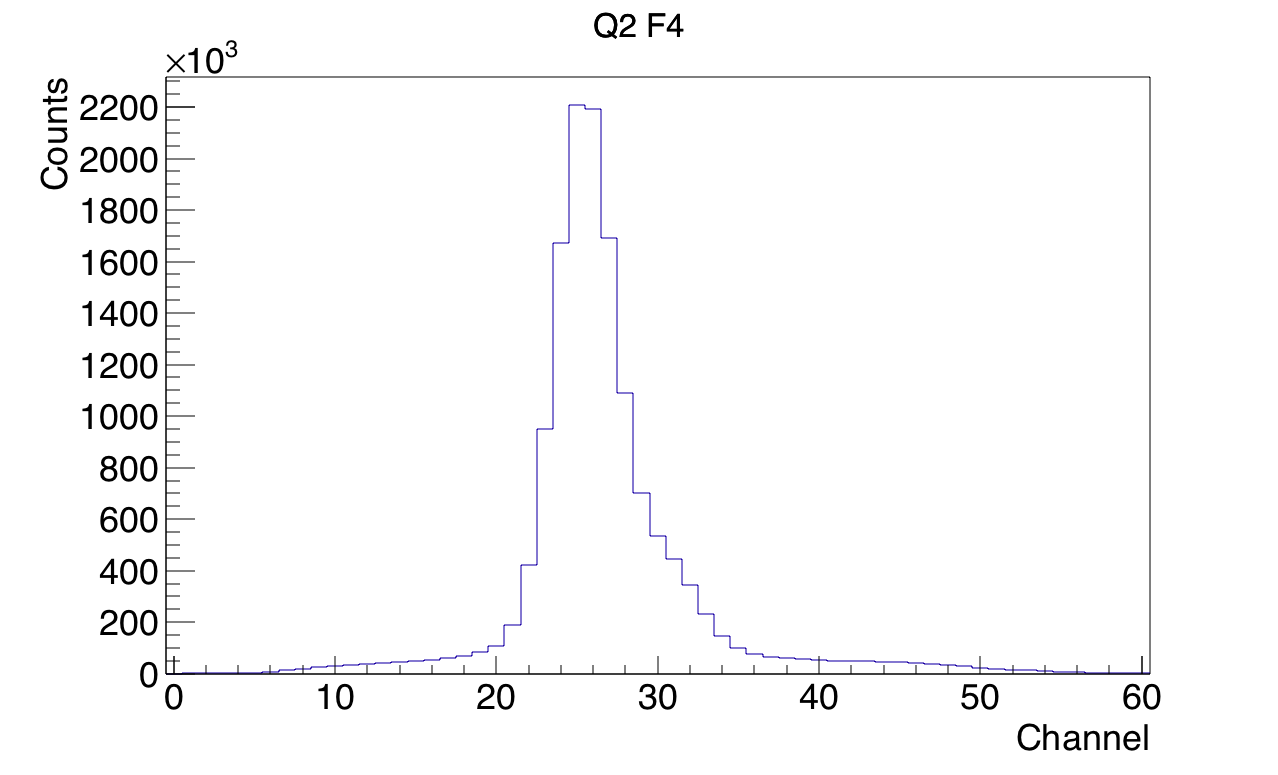
\includegraphics[width=\textwidth]{../Plots/plotting/Pedestal_Q2_f4.png}
%		\caption{Pedestal from annular strip 4 in quadrant 2.}
%		\label{fig:Pedestal_f}
%	\end{subfigure}
%	\begin{subfigure}{\textwidth}
%		\centering
%		% ParticlePlot.cpp
%		% check_pedestal("setup_Sm.txt", "b", 3, 8, 70)
%		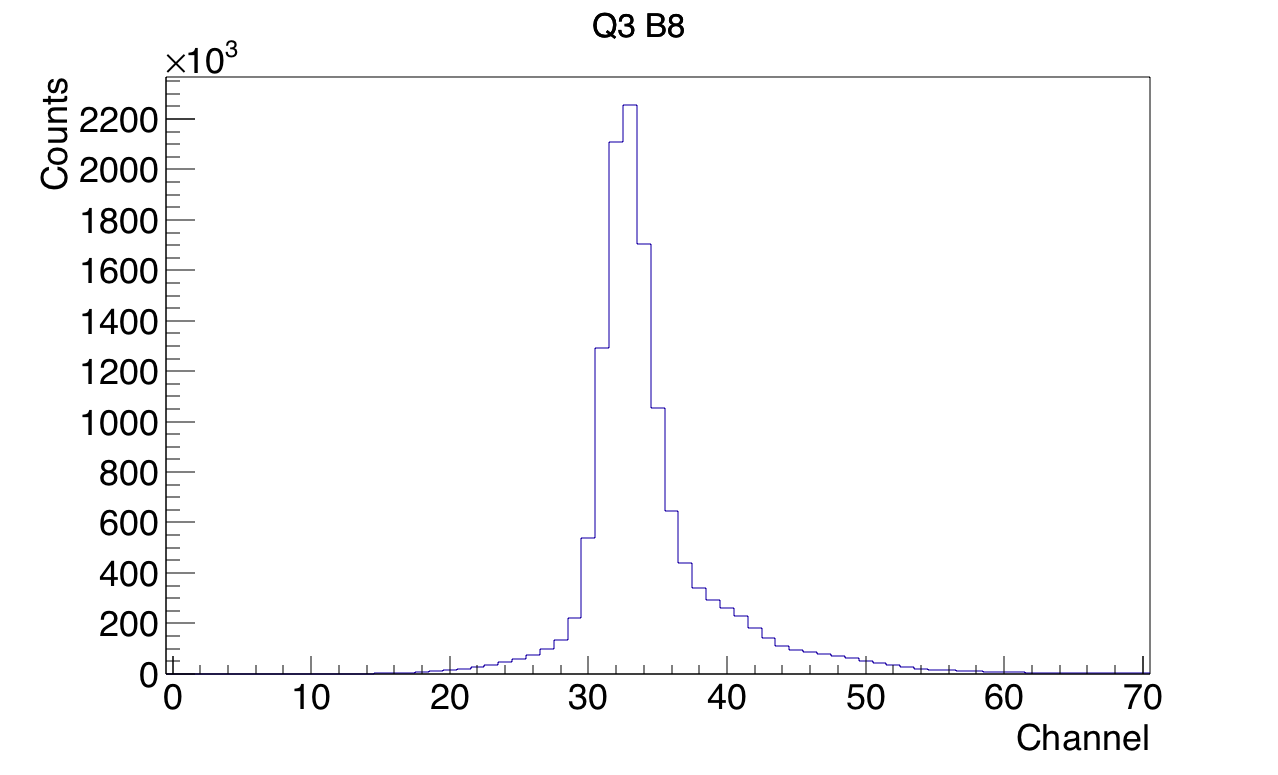
\includegraphics[width=\textwidth]{../Plots/plotting/Pedestal_Q3_b8.png}
%		\caption{Pedestal from radial strip 8 in quadrant 3.}
%		\label{fig:Pedestal_b}
%	\end{subfigure}
%	\caption{The pedestal from charge sharing in the front and back side of the CD.}
%	\label{fig:Pedestal}
%\end{figure}

%% BIG FIGURE, 4 plots ++

%\begin{figure}[ht]
%	\centering
%	\begin{subfigure}{\textwidth}
%		\centering
%		% ParticlePlot.cpp
%		% check_single_threshold("setup_Sm.txt", "f", 1, 11, 2100, 1500)
%		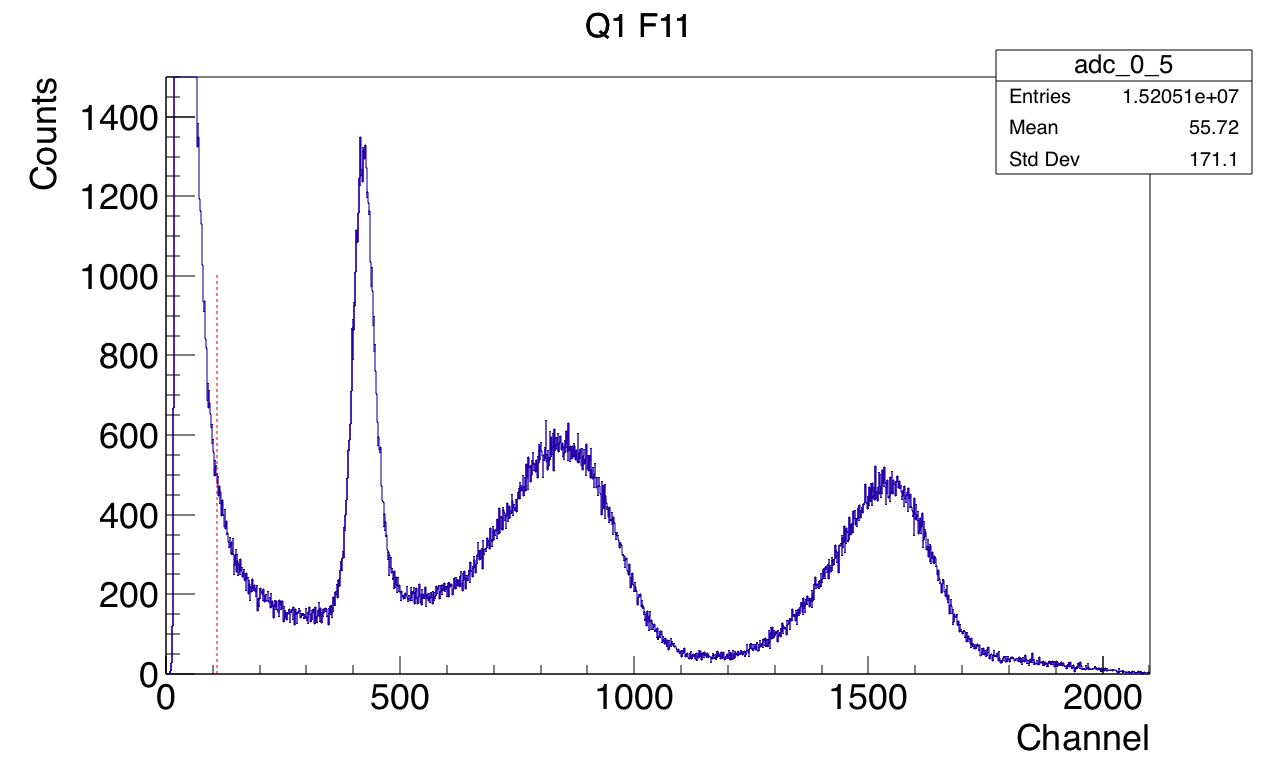
\includegraphics[width=\textwidth]{../Plots/plotting/Threshold_Q1_f11.png}
%		\caption{Annular strip 11 in quadrant 1.}
%		\label{fig:Threshold_f}
%	\end{subfigure}
%	\begin{subfigure}{\textwidth}
%		\centering
%		% ParticlePlot.cpp
%		% check_single_threshold("setup_Sm.txt", "b", 1, 6, 2800, 1500)
%		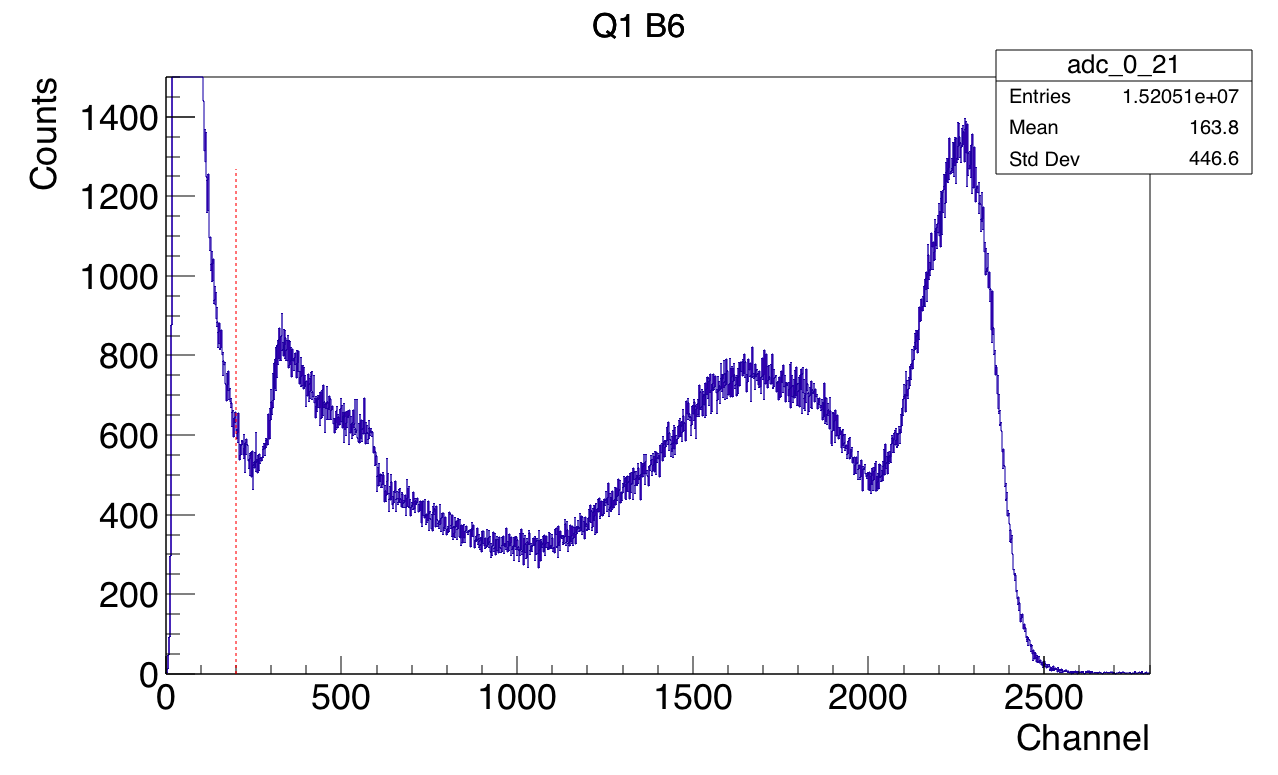
\includegraphics[width=\textwidth]{../Plots/plotting/Threshold_Q1_b6.png}
%		\caption{Radial strip 6 in quadrant 1.}
%		\label{fig:Threshold_b}
%	\end{subfigure}
%	\caption{The threshold, marked with a red dotted line, set for one front and one back strip of the CD.}
%	\label{fig:Threshold}
%\end{figure}

%\begin{figure}[ht]
%	\centering
%	% ParticlePlot.cpp
%	% energy_vs_ring("setup_Sm.txt")
%	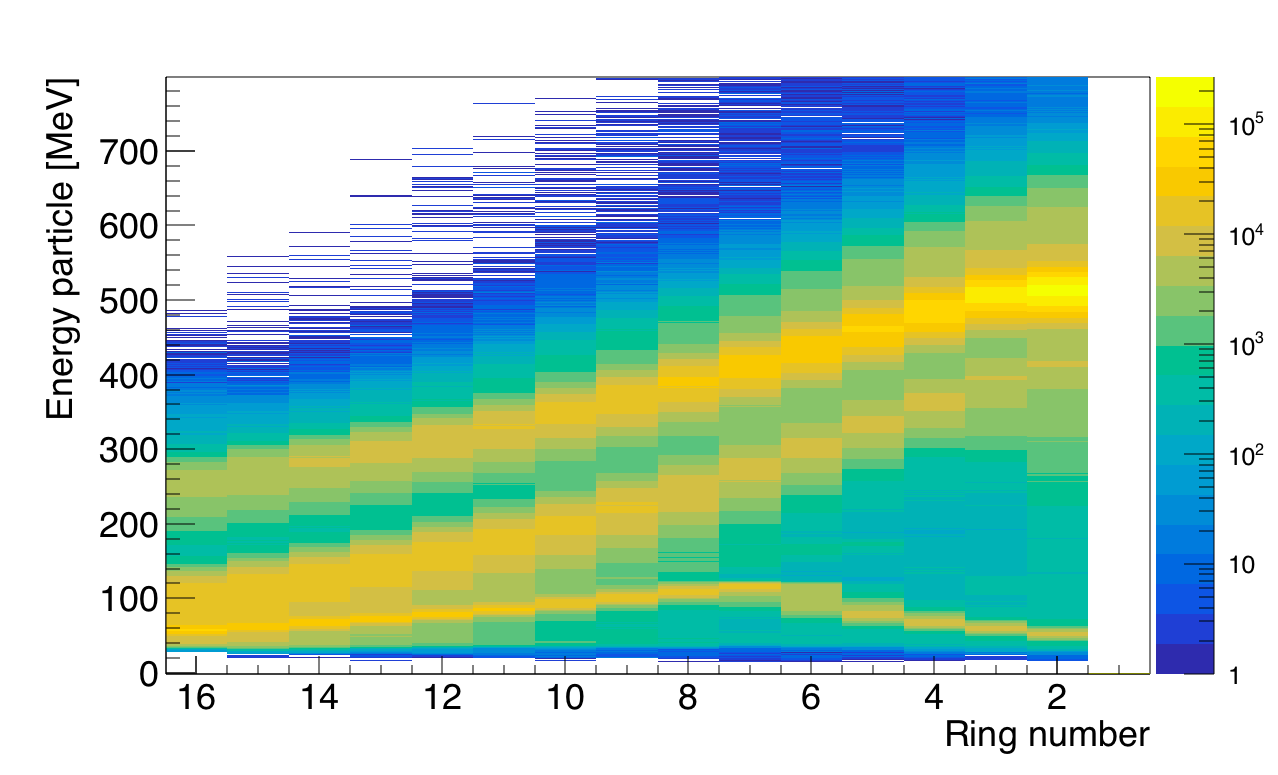
\includegraphics[width=\textwidth]{../Plots/plotting/E_vs_ring_all.png}
%	\caption{Energy vs. ring number all quadrants of the CD combined. The upper yellow curve is \Sm, the middle one is \Pb\ and the lower one is the contaminant. Ring 1, which is removed, is the innermost ring and ring 16 is the outermost ring.}
%	\label{fig:part}
%\end{figure}

\subsection{Calibration of the \texorpdfstring{$\gamma$}{gamma} detectors}\label{ssec:gamma}

%The online calibration is designed in such a way that the calibration of the \ga\ detectors is quite acceptable in a certain energy range.


During the setup of the experiment, a hardware and software calibration of the gamma detectors was performed by the ISOLDE staff, as stated in \autoref{ssec:online_cal}. 
The gains and offsets of each DGF were provided in such a way that the online analysis is more straightforward. 
In addition, it is easier to monitor the data on-line. 
However, the \ga\ detectors have non-linear properties, and the offsets and gains may drift over time, calling for a proper calibration. 
Therefore, a calibration run using $^{133}$Ba and $^{152}$Eu was performed at the end of the experiment. 
The $^{133}$Ba and $^{152}$Eu sources were placed in the target position simultaneously, back to back. 
With the data set from the source run, it possible to verify the quality of the online calibration, and if needed, perform a second calibration. 
In addition, the data from the calibration run can be used to determine the relative efficiency of the Miniball spectrometer.

To investigate the gamma calibration, all of the 144 gamma detector segments from the source run was plotted on top of each other, as displayed in \autoref{fig:gamma_comparison}. 
The alignment of the segments is excellent, i.e. there is no need to improve the gamma calibration. 
Even if the resolution had been improved by 0.1 keV by applying the source data, once the Doppler broadening gets into play, it makes no difference. 
Therefore, the online calibration was applied in the present thesis work, similar to the particle calibration.

\begin{figure}[ht]
	\centering
	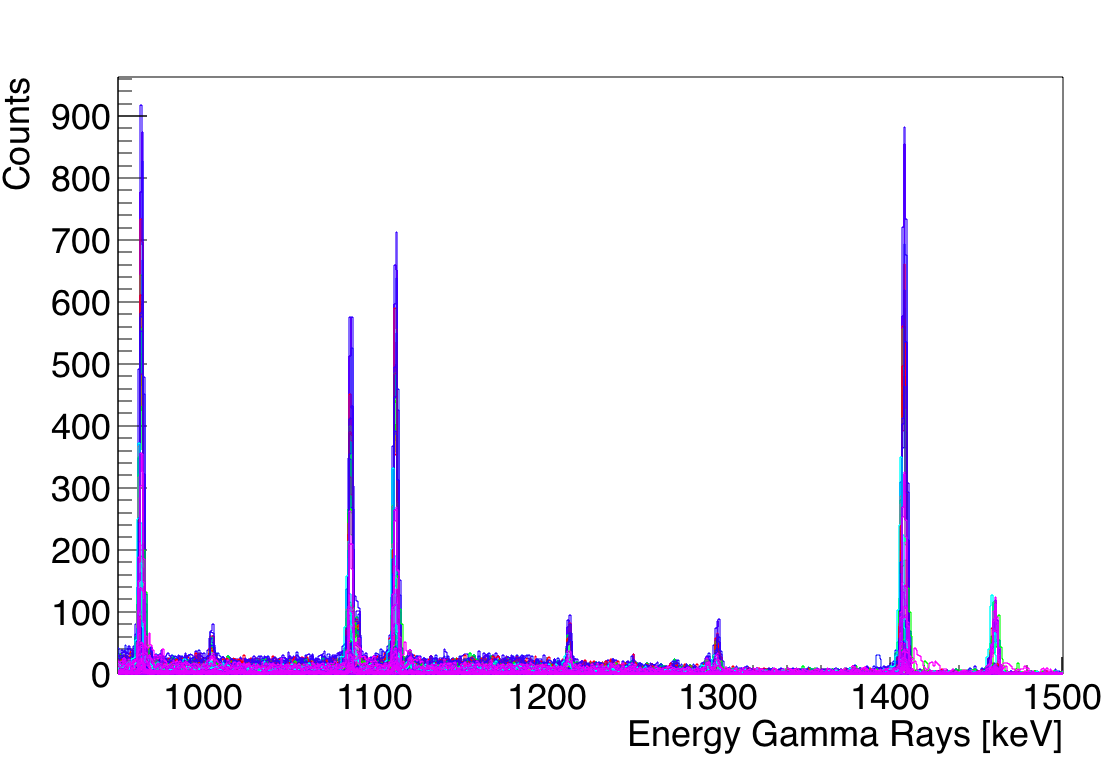
\includegraphics[width=\textwidth]{../Plots/comparing/gamma_comparison_full.png}
	\caption{Comparison of all 144 \ga\ detector segments from the source run with $^{133}$Ba and $^{152}$Eu. 
	Each of the 8 clusters are displayed with a different color.}
	\label{fig:gamma_comparison}
\end{figure}

The original thesis project included the calibration of the \ga\ detectors by means of an automatic fitting procedure.
For reasons explained in \autoref{ssec:user_cal}, the fitting procedure was abandoned.
Nonetheless, the expected program flow including the automatic fitting will be outlined in the following.

In the calibration run, there are many \ga\ lines for both Eu and Ba. 
Therefore, many data points can be applied in the calibration.
The fit can either be linear or quadratic, depending on the detector specification.
A simple linear calibration, with only two centroids can be performed similarly to the particle detector calibration.
From \autoref{eq:offset} and \autoref{eq:gain} we have
\begin{align}\label{eq:GGandA}
	g_\gamma &= \frac{E_{\text{Eu}} - E_{\text{Ba}}}{n_{\text{Eu}} - n_{\text{Ba}}} 
	&  
	a &= E_{\Gamma} - g_\gamma \cdot n_{\Gamma}
\end{align}
where $\Gamma$ can be peaks from either Eu or Ba.

The gray boxes in \autoref{fig:cal_FC} emphasizes the program flow of the \ga\ detector calibration. 
The idea is to use the \texttt{Q4S.sh} script to sort the experimental data with \texttt{TreeBuilder}.
Then, the \ga\ histograms are analyzed by means of ROOT using the \texttt{GammaPlot.cpp} script.
Histograms used for \ga\ detector calibration sorted by \texttt{TreeBuilder} use the naming convention $\textit{E\_gam\_seg}\_c\_d\_s$, where $c \in [0, 7]$ is the cluster number, $d \in [0, 2]$ is the detector number and $s \in [0, 6]$ is the segment number.
The core signal is $s = 0$ as displayed in \autoref{fig:HPGe}.

To perform the fitting, \texttt{GammaFit.cpp} would require the energy centroids as input. 
This script was never written, but the general idea is similar to the particle calibration.
Currently, the Python scripts \texttt{DGF\_generator.py} and \texttt{Geometry\_generator.py} reproduces the calibration coefficients and geometry parameters from the online calibration. 
These scripts need to be modified if a second, improved calibration is performed.
The final output of the \ga\ calibration would then have been pasted into the calibration file \textit{IS558-user.cal}.
After the calibration coefficients and the geometry parameters are added to the calibration file, the \texttt{TreeBuilder} program have to be re-run, utilizing the updated calibration file.



\subsection{\texorpdfstring{$\gamma$}{gamma} sorting}
After the completion of the calibration file, the next step is to run \texttt{CLXAna}.
\texttt{CLXAna} sorts the \ga\ spectra, makes a kinematic reconstruction to get the angle of the particles, and applies the Doppler correction in order to get the Doppler-corrected \ga-spectra to analyze the Coulomb excitation of \Sm.
The theory of the Doppler correction is explained in \autoref{ssec:Doppler}.
%\texttt{CLXAna} makes event trees and energy spectra for both particle and \ga\ detection which can be used for analyzing the Coulomb excitation events.

There are three methods of sorting the events from Miniball in \texttt{CLXAna}; singles, add-back and reject. 
When applying the singles method, every \ga-ray entering a detector is counted as an event.
There are no assumptions of Compton scattering in this kind of sorting. 
This implies that some of the events counted as true events are in fact scattered \ga's corresponding to a different energy.

The timing resolution cannot distinguish true \ga-\ga\ events from Compton scattering events.
When utilizing the add-back method, events occurring in neighboring detectors in the same cluster within a 100 ns time window are added together as a single event. 
The energies of the events that occurred in the separate segments are summed, and the segment with the highest energy is assumed to be the position of the incident \ga-ray.
An advantage of the add-back method is that the full energy of a single \ga-ray, which has undergone a Compton scattering process, can be reconstructed to increase the efficiency.
A disadvantage of the method is the uncertainty in the assumptions of the addition of several events into a single event. 
The add-back method can cause an increase in the intensity of \ga-ray sum peaks.
When utilizing the add-back method, in some cases two individual \ga-rays are added together, making the sum peak energy higher.
Thus no correction is performed when separate \ga-rays are added together in the detector \cite{Gaffney, MB-spect}.

When applying the reject method for the sorting, all events occurring in neighboring detectors in the same cluster within a 100 ns time window is excluded as an event. 
The total statistics will therefore be smaller when the reject method is applied. 
If the amount of total statistics is large, it is possible, or perhaps even an advantage to apply the reject method, as it will give a higher probability of getting the true full energy peaks of the detected \ga-rays. 

\texttt{CLXAna} has to be run twice in order to complete the sorting correctly.
In the first run, every input parameter except the graphical cuts have to be provided.
\autoref{fig:part_wcut} shows the cuts of the beam and target for the detected particle events.
These graphical cuts are used in the Doppler correction of the \ga-rays.
\autoref{ch:MBCS_ROOT} goes through the details of how the graphical cuts are obtained.
When the graphical cut file is made, the second run of \texttt{CLXAna} can be completed. 
In order to not copy and paste all commands into the command line, a script named \texttt{Coulex.sh} was made to sort the data with \texttt{CLXAna}. 
It uses the configuration file \textit{config-IS558.dat} and the graphical cut file \textit{outputfile.root}. 
In addition, it takes one command line flag, specifying the sorting method:
\begin{lstlisting}[language=]
'-s' (singles) 
'-a' (addback) 
'-r' (reject)
\end{lstlisting}
If no command line flag is given, the singles method is used by default.
An example of running the script and the output given by \texttt{CLXAna} is shown below
\begin{lstlisting}[language=]
$ ./Coulex.sh -s
--- Coulex: singles ---
Input parameters:
Zb = 62
Ab = 140
Zt = 82
At = 208
Eb = 4650 keV/u
Ex = 531 keV
thick = 1.4 mg/cm2
depth = 0.7 mg/cm2
cddist = 27 mm
cdoffset = 242.6 degrees
deadlayer = 0.0007 mm
contaminant = -1 mg/cm2
spededist = 23.6 mm
bg_frac = -0.75
srim = /Users/trondwj/GitHub/MasterThesis/SRIM
cutfile = ../../Sorted_data/outputfile.root:Bcut:Tcut
Begin g_clx loop.
Info in <TCanvas::Print>: pdf file /Users/trondwj/GitHub/MasterThesis/SRIM/140Sm_208Pb.pdf has been created
Info in <TCanvas::Print>: pdf file /Users/trondwj/GitHub/MasterThesis/SRIM/208Pb_208Pb.pdf has been created
Info in <TCanvas::Print>: pdf file /Users/trondwj/GitHub/MasterThesis/SRIM/140Sm_Si.pdf has been created
Info in <TCanvas::Print>: pdf file /Users/trondwj/GitHub/MasterThesis/SRIM/208Pb_Si.pdf has been created
Initialising histograms...
Looping over events...
Warning in <TClass::Init>: no dictionary for class trevts is available
1-particle events = 89020258%)    
Finished.
\end{lstlisting}
A detailed explanation of the input parameters is provided in \autoref{ch:MBCS_ROOT}.

\begin{figure}[htb]
	\centering
	\begin{subfigure}[t]{0.49\textwidth}
		\centering
		% GammaPlot.cpp
		% particle_events_with_cut()
		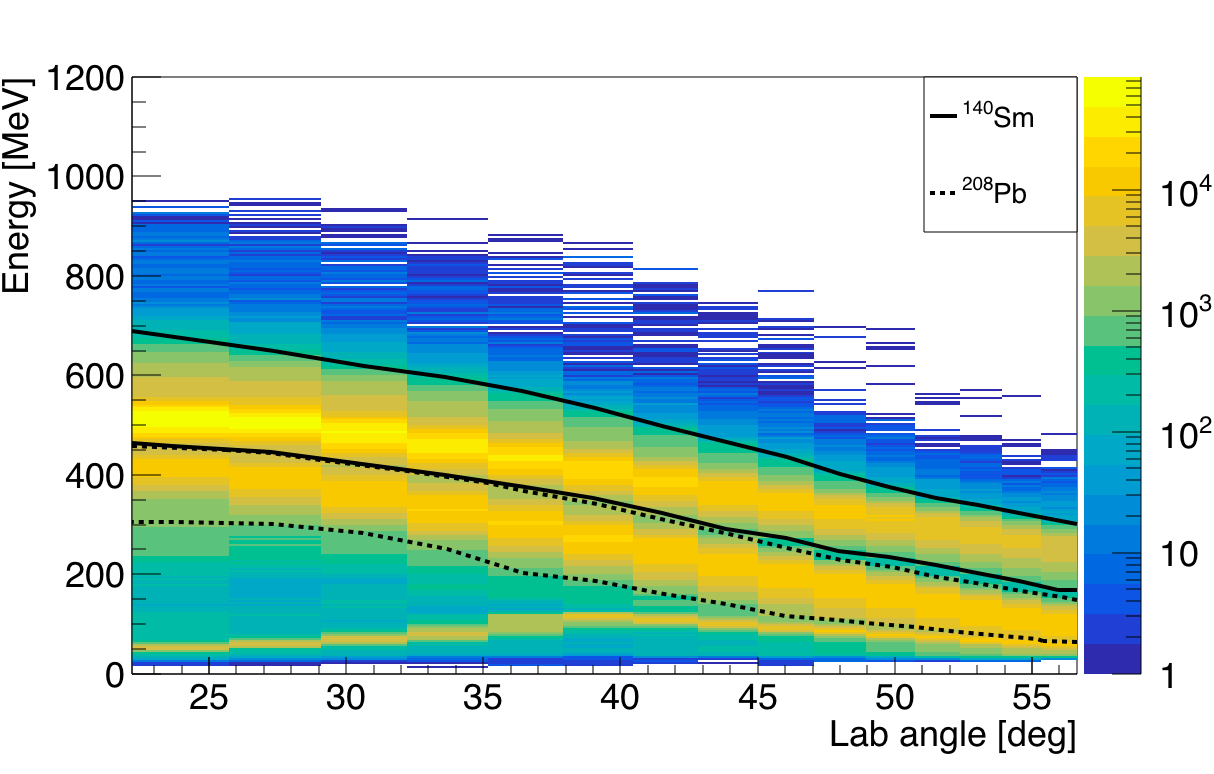
\includegraphics[width=\textwidth]{../Plots/plotting/particle-events-wcut.png}
		\caption{}
		\label{fig:part_wcut}
	\end{subfigure}
	\hfill 
	\begin{subfigure}[t]{0.49\textwidth}
		\centering
    		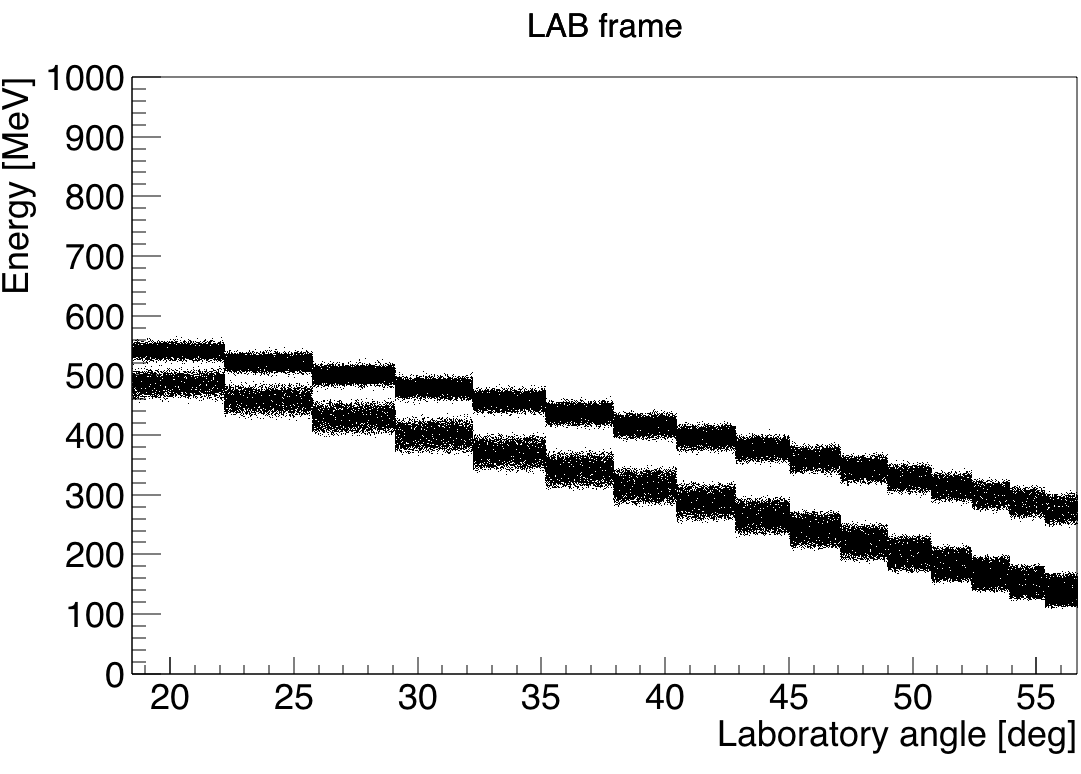
\includegraphics[width=\textwidth]{../Plots/simulation/kin_140Sm_208Pb.png}
		\caption{}
		\label{fig:kinsim}
	\end{subfigure}
	\caption{Detected and simulated particle events of \Sm\ on \Pb\ at 4.65 MeV/u in the LAB frame. Smaller angles corresponds to the inner rings and larger angles to the outer rings.
	\textbf{(a)} The data enclosed by the solid upper and dotted lower lines are the detected particle events of Sm and Pb, respectively. 
	At smaller angles it is difficult to separate the lower solid line from the upper dotted line, but this is visible at larger angles.
	Underneath and outside the Pb area, the contaminant is displayed in yellow.
	\textbf{(b)} The simulated kinematics, where the upper curve corresponds to Sm events and the lower curve corresponds to Pb events.
	}
	\label{fig:part_events}
\end{figure}


\autoref{fig:B_dcB_cid} shows that the Doppler correction works nicely.
If there was anything wrong with the detector angles, it would not display lines at certain energies after the Doppler correction. 
Also the width of the lines indicates that the particle calibration is quite good. 
If there were systematic deviations in the particle calibration, it would have shown up as irregularities in this plot.

\begin{figure}[ht]
	\centering
	% GammaPlot.cpp
	% beam_gated_dcB_gammas_core("setup_Coulex.txt", "d")
	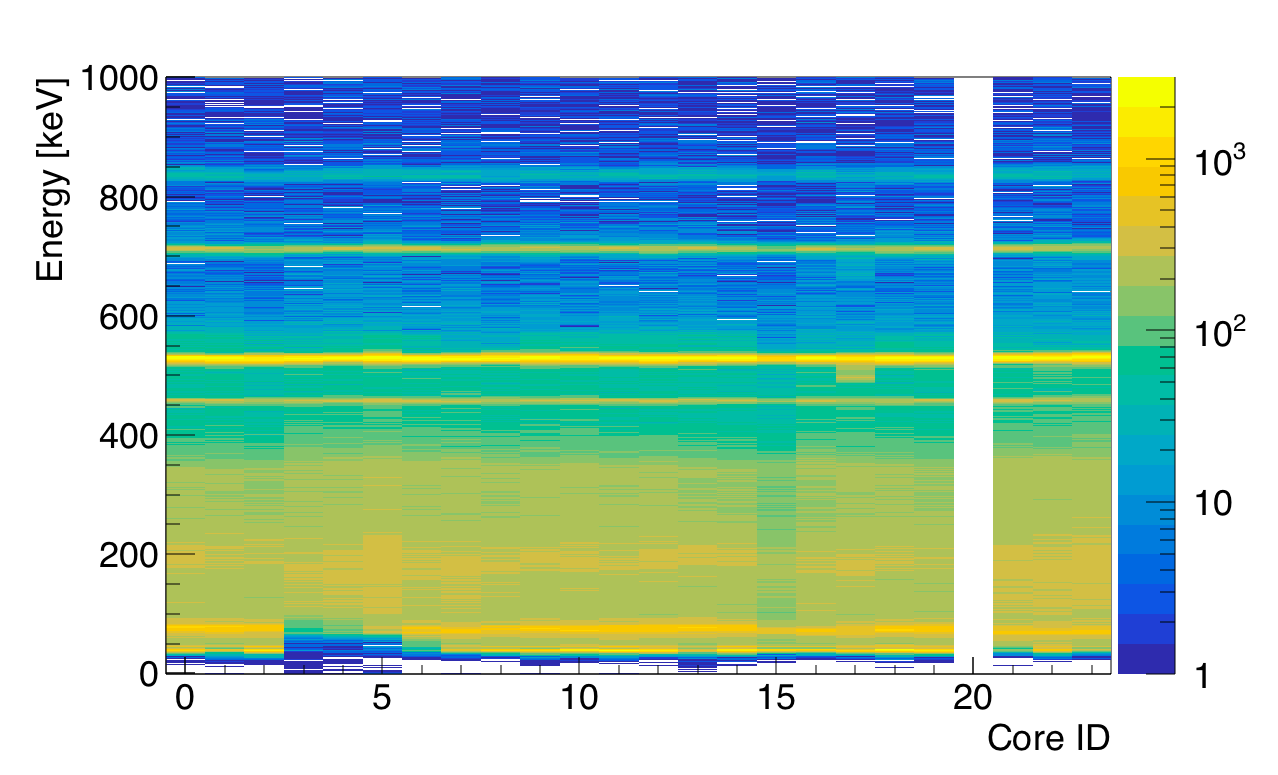
\includegraphics[width=\textwidth]{../Plots/plotting/B_dcB_cid.png}
	\caption{Beam gated prompt, Doppler corrected \ga-rays from \texttt{CLXAna}. Core ID 20 is removed, see \autoref{sec:BDS}. \textcolor{blue}{Perhaps add a similar plot for the source data (without DC of course)?} \textcolor{red}{This is not source data...}}
	\label{fig:B_dcB_cid}
\end{figure}


%\autoref{tab:DGF}, \textcolor{red}{not sure how to make this table. How is the histogram names and the calibration coefficients linked? Not exactly straightforward.}
%\begin{table}[ht] 
%	\centering 
%	\caption{DGF}
%	% Data for the DGF table
\begin{tabular}{cccc}
\hline
Cluster & Detector & Segment & TreeBuilder            \\
\hline
0       & 0        & 0       & E\_gam\_seg\_0\_0\_0   \\
\hline
\end{tabular}
%	\label{tab:DGF}
%\end{table}

%The Miniball spectrometer \cite{MB-spect} \newline
%p. 8: \newline
%\textbf{Efficiency and resolution:}
%left bottom: \newline
%The application of an add-back (AB) routine involves the summing of the energies of two coincident gamma rays within 100 ns in neighboring cores on the same cluster detector. This situation corresponds to a Compton-scattered \ga-ray event where the energy of the \ga-ray is shared between two or more crystals in the same triple cluster detector. For higher-energy \ga-rays, where scattering from one crystal into its neighbor is quite likely, this improves the efficiency, but for low-energy \ga-rays, where scattering is less likely, summing effects actually reduce the efficiency. For this reason a cut-off is normally applied and AB is only performed for energies above this threshold. \newline


\subsection{Doppler correction}\label{ssec:Doppler}
The scattered beam particles travel with a significant velocity.
When the particles de-excite, they emit \ga-rays which can be observed to have large Doppler shifts.
To get the correct \ga\ energies, a Doppler correction must be performed.

In order to perform the Doppler correction, the angles of the interaction points in the Miniball frame of reference has to be known. 
\autoref{fig:HPGe} shows a sketch of the Miniball cluster geometry and the associated table gives the angles and distance of the different clusters.
The parameters $\theta$, $\phi$ and $R$ describes the position of the central axis of the detector clusters, while $\alpha$ describes the orientation about the axis of the cluster. 
All these parameters are required to calculate the position of the segments or the position of a point determined by the pulse-shape analysis, and have to be added to the calibration file. 
The interaction point is determined either from the segment with the largest energy or using a pulse-shape analysis. 
%In the first case, the position of the center of each segment has to be known.
%In the second case, geometrical information to relate the time-to-steepest slope and ratio of the mirror charge amplitudes to the angle between the interaction point, the target and the emitted particle need to be known. 
These geometrical calculations are built into \texttt{MiniballCoulexSort}.

Because of the significant velocity of the scattered particles, the emitted \ga-rays from the particle de-excitation has a Doppler shifted \ga\ energy given by 
\begin{equation}\label{eq:DS}
	E_\gamma = \frac{E_\gamma^{'}}{\gamma (1 - \beta \cos \theta)}
\end{equation}
where $E_\gamma$ is the \ga\ energy detected in the LAB frame, $E_\gamma^{'}$ is the \ga\ energy in the nucleus' frame of reference, $\beta = \frac{v}{c}$, $v$ is the nucleus' velocity, $c$ is the speed of light, $\theta$ is the angle of the emitted \ga-ray with respect to the nucleus' direction of motion and $\gamma = 1/\sqrt{1 - \beta^2}$ is the Lorentz factor. Since both the CD and the HPGe array are segmented, the emission angle $\theta$ of the \ga-ray can be calculated by 
\begin{equation}\label{eq:DSA}
	\cos \theta = \sin \theta_p \sin \theta_\gamma \cos (\phi_p - \phi_\gamma) + \cos \theta_p \cos \theta_\gamma
\end{equation}
where ($\theta_p, \phi_p$) and ($\theta_\gamma, \phi_\gamma$) are the detection angles of the particle and \ga-ray respectively, ($\theta_p, \theta_\gamma$) are the angles with respect to the beam axis and ($\phi_p, \phi_\gamma$) are the azimuthal angles \cite{RIBF2012, MB-spect}. The Doppler correction factor is found by combining \autoref{eq:DS} and \autoref{eq:DSA} into
\begin{equation}
	\frac{E_\gamma^{'}}{E_\gamma} = \gamma (1 - \beta (\sin \theta_p \sin \theta_\gamma \cos (\phi_p - \phi_\gamma) + \cos \theta_p \cos \theta_\gamma))
\end{equation}





\subsection{Broken detector segments}\label{sec:BDS}

Si detectors are known to obtain deficiencies when they are old due to the bombardment of the particles from several experiments.
In fact, the CD was scheduled to be replaced after our experiment. 
As a result of the kinematics of the setup, the innermost ring of the CD is the most vulnerable as it receives the highest energy impact. 
As presented in \autoref{fig:BDS_R1}, it is not possible to separate the beam and target peaks of ring number 1. 
For this reason, all counts obtained in ring number 1 was removed entirely from the data set.
This was very unfortunate since the innermost ring collected the most statistics.

As \autoref{fig:EFBQ4} shows, the calibration of the CD got better by removing the innermost ring. 
The most visibly lines which did not fit $y = x$ vanished, implying that most of the problem was in fact the coefficients of ring 1.

On the back side of the CD, one pixel had an abnormal behavior compared to the other back strips in the same quadrant. 
Presented in \autoref{fig:BDS_B1}, radial strip 1 (B1) gated on annular strip 16 in quadrant 4 showed a lot more counts than all of the other strips combined. 

In addition, there were several other incidents where B1 presented an irregular behavior, though not as striking as the case discussed above.
We considered to exclude B1 from the data set, but given that the pixel are in the outermost region of the CD, not giving loads of counts, we decided not to.
There were not any visible effects in \autoref{fig:EFBQ4} by keeping B1.

\begin{figure}[ht]
	\centering
	\begin{subfigure}[t]{0.49\textwidth}
		\centering
		% ParticlePlot.cpp
		% get_single_plot("setup_Sm.txt", "tb", "f", 0, 1, 1, 1, 0, 2500, 8000)
		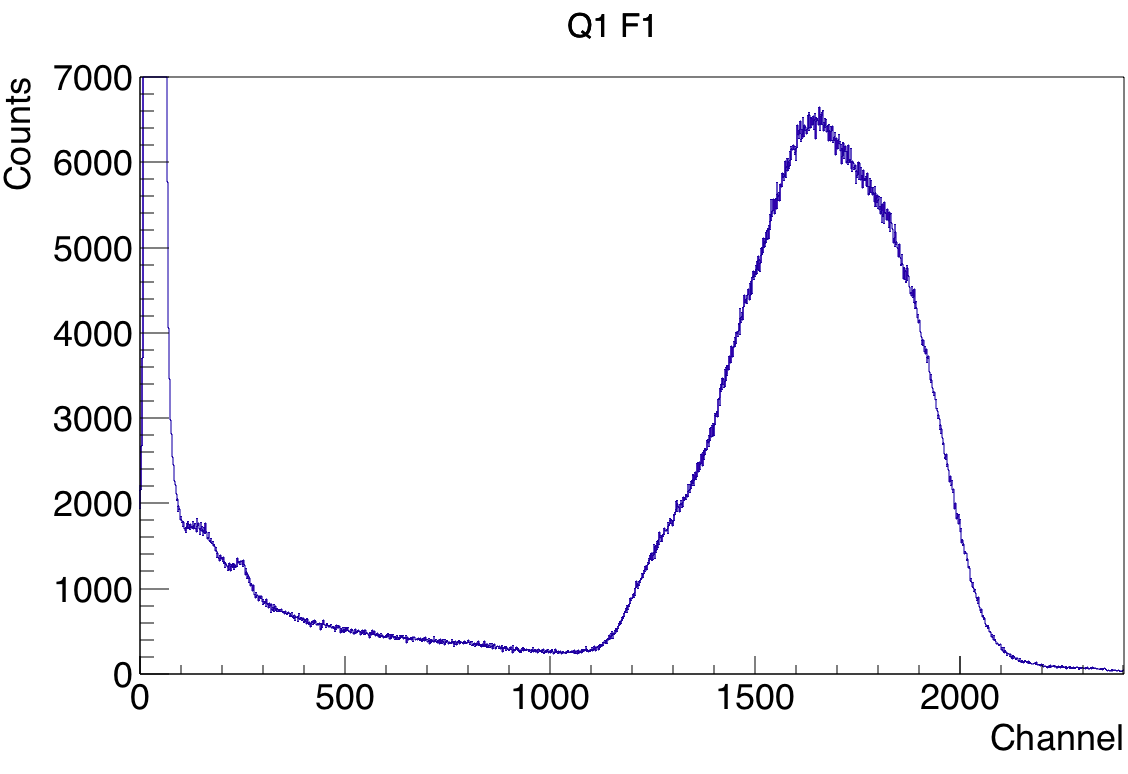
\includegraphics[width=\textwidth]{../Plots/plotting/TB_Q1_F1.png}
		\caption{}
		\label{fig:BDS_R1}
	\end{subfigure}
	\hfill
	\begin{subfigure}[t]{0.49\textwidth}
		\centering
		% ParticlePlot.cpp
    		% plot_back_strips("setup_Sm.txt", 4, 16, 0, 0, 1700, 400)
		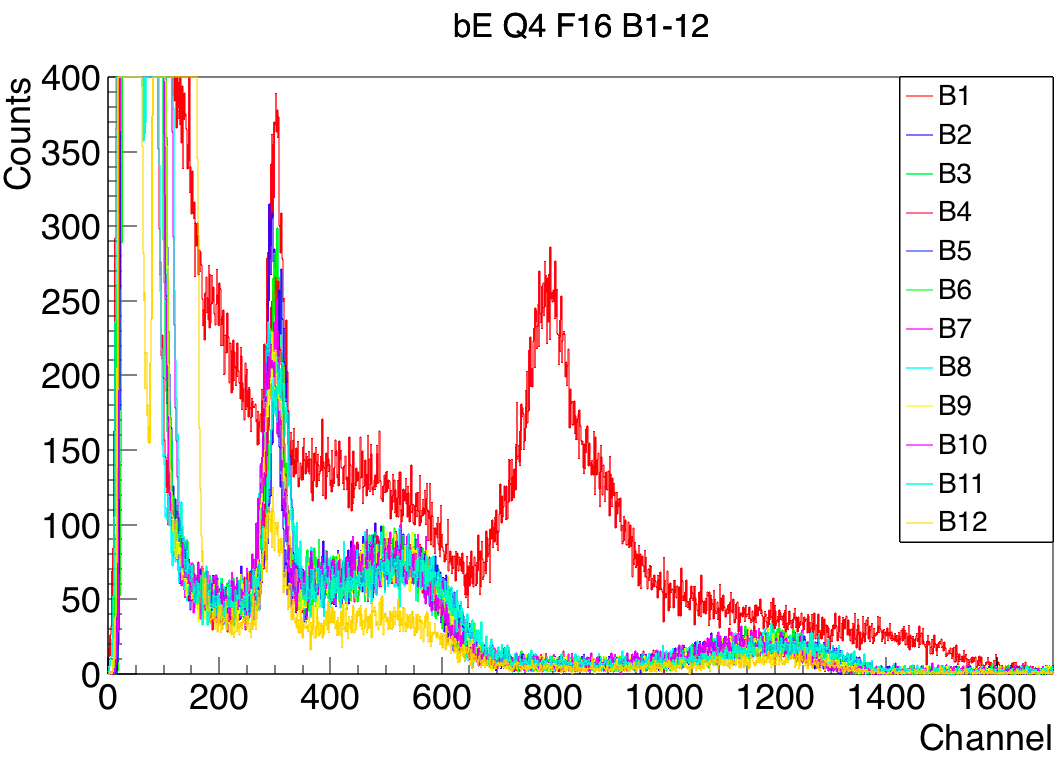
\includegraphics[width=\textwidth]{../Plots/plotting/bE_Q4_f16_b1-12.png}
		\caption{}
		\label{fig:BDS_B1}
	\end{subfigure}
	\caption{Broken detector strips in the CD.
	(a) Ring 1 in quadrant 1. It is impossible to separate \Pb\ from \Sm.
	(b) CD back strip 1 gated on front ring 16 (outermost ring) in quadrant 4. B1 shows a lot more counts than the other strips arount channel 800.}
	\label{fig:BDS}
\end{figure}

From earlier experiments, the ISOLDE staff had observed a few broken detector segments of the \ga\ detector.
In \autoref{fig:B_dcB_cid}, core ID 20 was removed due to a broken segment. 
In addition, Core ID 15 displays fewer counts than the neighboring detectors.
This is due to a crosstalk issue involving a dead segment in detector 18A (cluster 5, core 0, segment 1 and 2). 
Crosstalk is the phenomenon where a signal transmitted on one channel creates an undesired effect in another channel. 
It means that some events had to be rejected.
% to avoid double-peaking, and this reduces the efficiency.

In order to exclude a detector segment, the gain and offset is simply set to -1, or the gain is set to 0 and the offset to -1.
It causes the energy calibration to become negative, and the faulty detector segment falls out of the scope. 
%It is the way it is usually done for dead CD strips or dead \ga\ detectors. 


%\begin{figure}[ht]
%	\centering
%	\begin{subfigure}{\textwidth}
%		\centering
%		% plot_quadrants("setup_Sm.txt", "f", 1, 0, 1, 0, 3500, 8500)
%		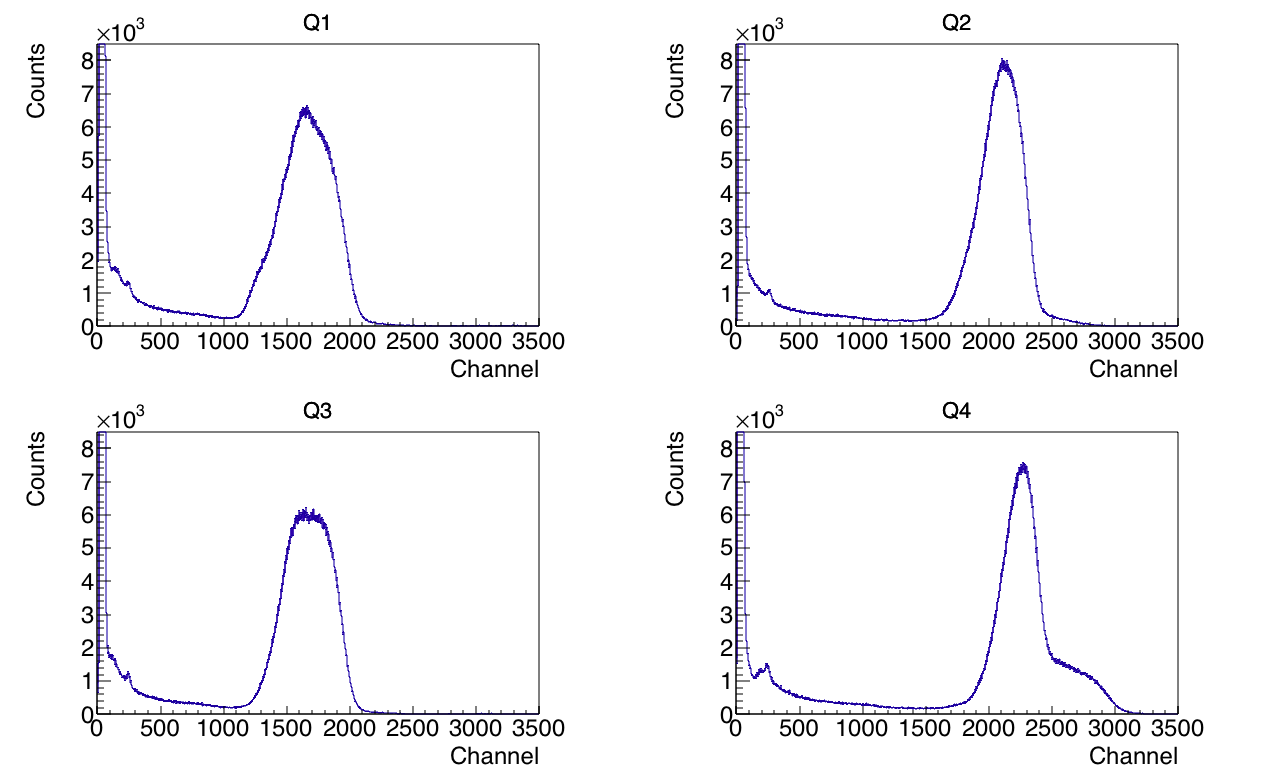
\includegraphics[width=\textwidth]{../Plots/plotting/Q1-4_f1.png}
%		\caption{CD front ring 1 (innermost ring). It is impossible to separate \Pb\ from \Sm.}
%		\label{fig:BDS_R1}
%	\end{subfigure}
%	\begin{subfigure}{\textwidth}
%		\centering
%		% plot_back_strips("setup_Sm.txt", 4, 16, 0, 0, 1700, 400)
%		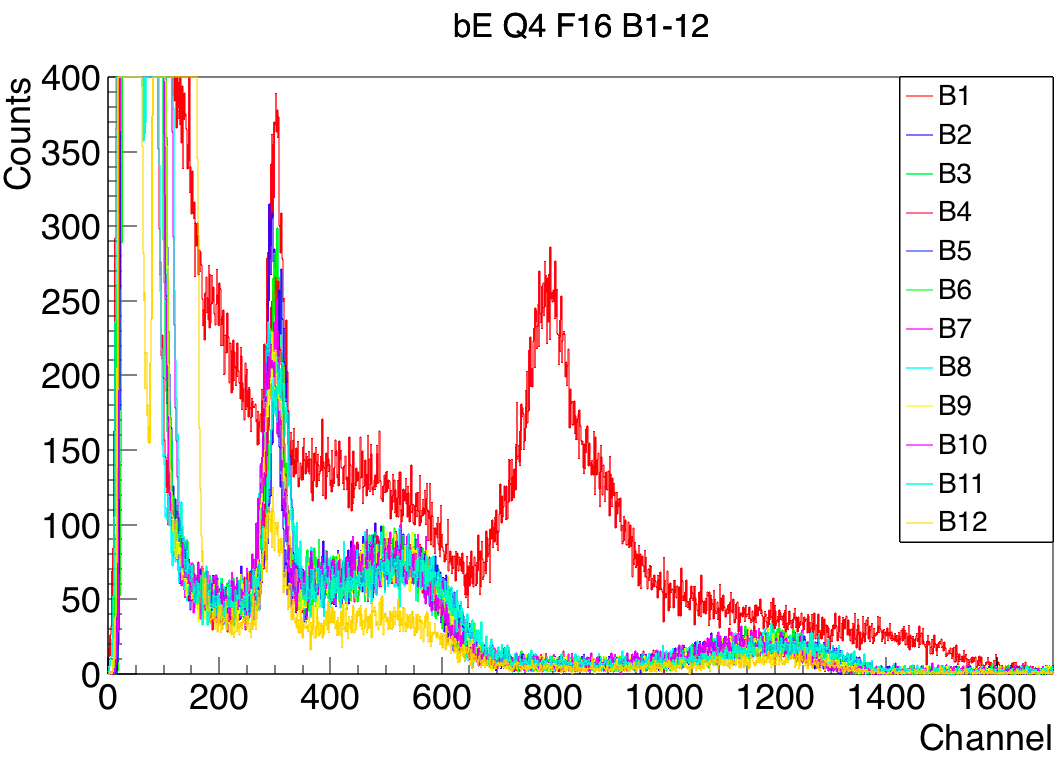
\includegraphics[width=\textwidth]{../Plots/plotting/bE_Q4_f16_b1-12.png}
%		\caption{CD back strip 1 gated on front ring 16 (outermost ring) in quadrant 4. B1 shows a lot more counts than the other strips arount channel 800.}
%		\label{fig:BDS_B1}
%	\end{subfigure}
%	\caption{Broken detector segments in the CD.}
%	\label{fig:BDS}
%\end{figure}

%\begin{figure}[ht]
%		\centering
%		% plot_back_strips("setup_Sm.txt", 4, 16, 0, 0, 1700, 400)
%		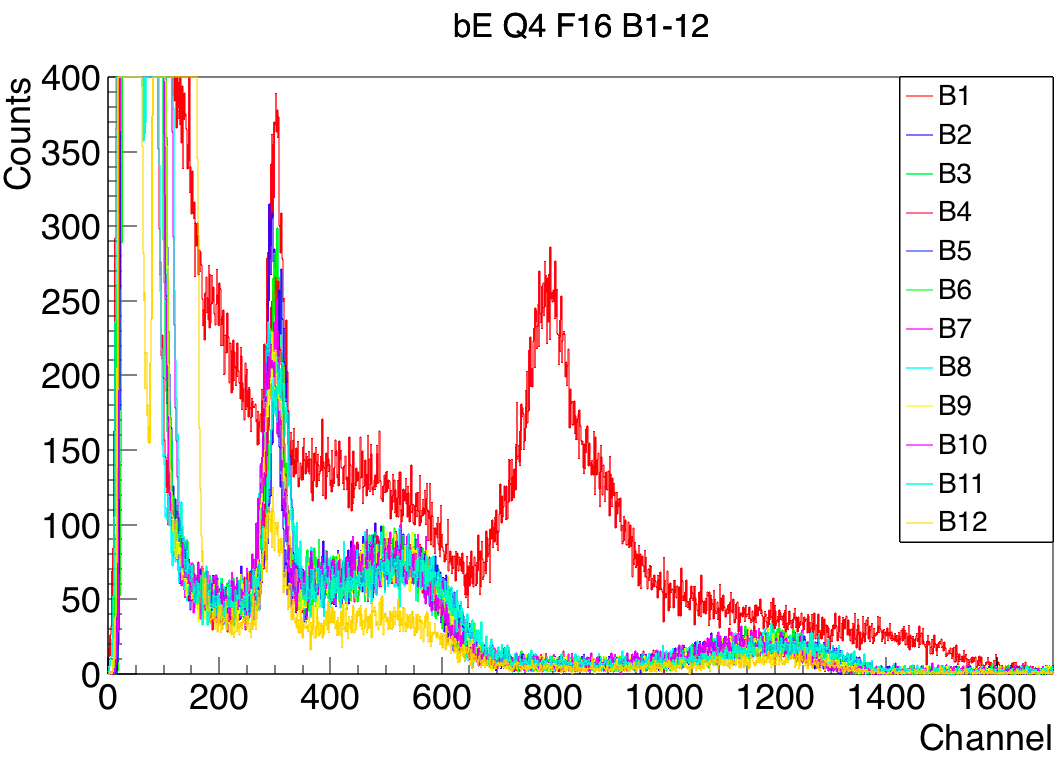
\includegraphics[width=\textwidth]{../Plots/plotting/bE_Q4_f16_b1-12.png}
%		\caption{CD back strip 1 gated on front ring 16 (outermost ring) in quadrant 4. B1 shows a lot more counts than the other strips arount channel 800.}
%		\label{fig:BDS_B1}
%\end{figure}


%\begin{figure}[ht]
%	\centering
%	\begin{subfigure}[t]{0.49\textwidth}
%		
%	\end{subfigure}
%	\hfill
%	\begin{subfigure}[t]{0.49\textwidth}
%		
%	\end{subfigure}
%	\caption{}
%	\label{fig:???}
%\end{figure}


% ----------------------------------------------------------------------------------------------------------------------% ----------------------------------------------------------------------------------------------------------------------


\chapter{Experimental results and discussion}
\epigraph{\textit{"In physics, you don't have to go around making trouble for yourself – nature does it for you."}}{\textit{– Frank Wilczek}}


With the direction and energy (velocity) of the scattered particle and the direction of the \ga-ray, a Doppler correction can be performed under the assumption that the \ga-ray was emitted from the projectile. 
The total \ga-ray singles and add-back spectrum corresponding to the CM scattering angles between $36.6^\circ$ and $136.0^\circ$, Doppler corrected for the projectile is displayed in \autoref{fig:gam_dcB}. 
As a comparison, the total \ga-ray singles spectrum from the previous experiment (from 2012) is displayed in \autoref{fig:gam_MK}.
There is a lot more \ga\ transitions visible from the present experiment with the \Pb\ target in \autoref{fig:gam_dcB} compared to the previous experiment with the $^{94}$Mo target. 
By looking at the relative intensity of $2_2^+ \rightarrow 2_1^+$ (460 keV) compared to $2_1^+ \rightarrow 0_1^+$ (531 keV) in both \ga\ spectra, we see that the probability for multi-step excitations are much greater with the Pb target. \textcolor{red}{Kan man se dette direkte av intensiteten? Spiller ikke beam energien også en rolle her, 2.85 MeV/u vs. 4.65 MeV/u?}
When sorting the data with the add-back method, there is a visible enhanced efficiency for high-energy \ga-rays, the peaks are more distinct. 

\begin{figure}[htb!]
	\centering
	\begin{subfigure}[t]{\textwidth}
		\centering
		% GammaPlot.cpp
		% total_statistics("setup_Coulex.txt", "d")
		% total_statistics_s_and_a()
		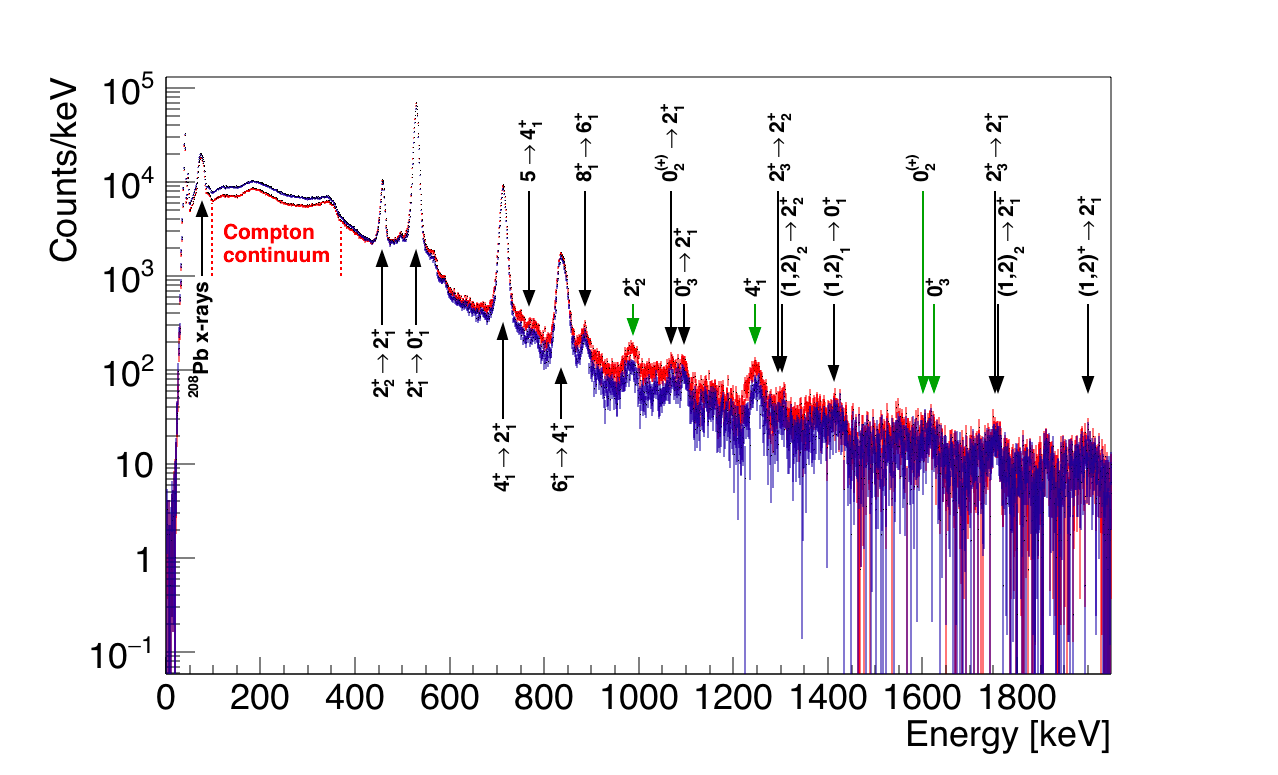
\includegraphics[width=\textwidth]{../Plots/plotting/gam_dcB_s_and_a.png}
		\caption{}
		\label{fig:gam_dcB}
	\end{subfigure}
	\begin{subfigure}[t]{0.8\textwidth}
		%\centering
		\blank{-1cm}
		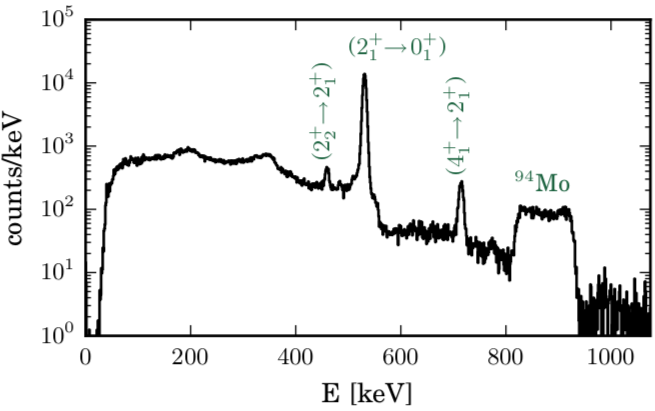
\includegraphics[width=\textwidth]{Images/gam_MK.png}
		\caption{}
		\label{fig:gam_MK}
	\end{subfigure}
	\caption{Background subtracted \ga\ spectrum, Doppler corrected for the scattered projectile (the beam).
		\textbf{(a)} \Sm\ on \Pb\ at 4.65 MeV/u from the COULEX experiment in 2017.
	 	The blue (red) \ga\ spectrum corresponds to sorting with singles (add-back) in \texttt{CLXAna}.
	 	% \ga\ spectrum in coincidence with a particle in the CD
		\textbf{(b)} \Sm\ on $^{94}$Mo at 2.85 MeV/u from the COULEX experiment in 2012.  
		See text for more information. \newline 	
	 	}
	\label{fig:gam_compared}
\end{figure}

The black arrows, except for the first one, in \autoref{fig:gam_dcB} corresponds to the known \ga\ transitions in \autoref{tab:gamma_trans}. 
The far right column of \autoref{tab:gamma_trans} shows which \ga\ transitions are visible in \autoref{fig:gam_dcB}.
At very low energy, pointed by the first black arrow below the Compton continuum, a peak of \Pb\ x-rays is visible. 
When the beam passes through the target, there is a possibility that electrons are removed, which produces x-rays when the holes are filled.

\begin{table}[htb!] 
    \centering 
    \caption{Known \ga\ transitions in \Sm\ based on \cite{Klintefjord, NNDC-levels}. 
    $E$ refers to the energy, $J^\pi$ is the spin and parity, $I_\gamma$ is the \textcolor{red}{??? \ga\ intensity ??? Hvis det er intensitet, skal ikke den da summere til 100 innenfor en tilstand? Noen er jo 100, mens andre overganger fra samme tilstand er mindre enn 100.} and $\sigma \lambda$ is the multipolarity. 
    The column "Visible in \ga\ spectrum" describes if it is possible to see the transition in \autoref{fig:gam_dcB}.}
	% Data for the Gamma transitions table
\begin{tabular}{ccccccccc}
\hline
\multicolumn{3}{c}{Initial level} & \multicolumn{3}{c}{$\gamma$ transition}    & \multicolumn{2}{c}{Final level}  & Visible in        \\
E        & $J^\pi$   & $T_{1/2}$  & $E_\gamma$ & $I_\gamma$ & $\sigma \lambda$ & E               & $J^\pi$        & $\gamma$ spectrum \\
{[keV]}  &           &            & [keV]      &            &                  & [keV]           &                &                   \\
\hline
0.0      & $~0^+$    &   14.82 m  &            &            &                  &                 &                &                   \\
530.68   & $~2^+$    &    6.10 ps &  530.7     & 100        & $E2$             &    0.0          & $~0^+$         & Yes               \\
990.37   & $~2^+$    &    7.7 ps  &  459.9     & 100        & $E2(+M1)$        &  530.68         & $~2^+$         & Yes               \\
1245.83  & $~4^+$    &    1.00 ps &  715.0     & 100        & $E2$             &  530.68         & $~2^+$         & Yes               \\
1420.31  & $(1,2)$   &            & 1420.3     & 100        &                  &    0.0          & $~0^+$         & Yes               \\
1598.79  & $0^{(+)}$ &            &  352.4     &   3.6      &                  & 1245.83         & $~4^+$         & No                \\
         &           &            &  608.6     &  17.3      &                  &  990.37         & $~2^+$         & No                \\
         &           &            & 1068.0     & 100        & $E2$             &  530.68         & $~2^+$         & Yes               \\
1628.39  & $~0^+$    &            & 1097.7     & 100        &                  &  530.68         & $~2^+$         & Yes               \\
1932.89  & $(0,1,2)$ &            & 1402.2     & 100        &                  &  530.68         & $~2^+$         & No                \\
2014.7   & $5$       &            &  768.8     & 100        &                  & 1245.83         & $~4^+$         & Yes               \\
2081.91  & $~6^+$    &            &  836.1     & 100        &                  & 1245.83         & $~4^+$         & Yes               \\
2283.89  & $~2^+$    &            &  685.1     &  47        &                  & 1598.79         & $~0^+$         & No                \\
         &           &            & 1293.6     &  63        &                  &  990.37         & $~2^+$         & Yes               \\
         &           &            & 1752.8     & 100        &                  &  530.68         & $~2^+$         & Yes               \\
         &           &            & 2283.9     &  26        &                  &    0.0          & $~0^+$         & No                \\
2289.64  & $(1,2)$   &            & 1299.4     &  75        &                  &  990.37         & $~2^+$         & Yes               \\
         &           &            & 1758.7     & 100        &                  &  530.68         & $~2^+$         & Yes               \\
         &           &            & 2289.1     &  50        &                  &    0.0          & $~0^+$         & No                \\
2326.4   & $7$       &            &  311.7     & 100        &                  & 2014.7          & $5$            & No                \\
2482.06  & $(1,2)^+$ &            &  882.7     &  10        &                  & 1598.79         & $~0^+$         & No                \\
         &           &            & 1491.3     & 100        &                  &  990.37         & $~2^+$         & No                \\
         &           &            & 1952.0     &  67        &                  &  530.68         & $~2^+$         & Yes               \\
2595.6   & $(0,1,2)$ &            & 2064.9     & 100        &                  &  530.68         & $~2^+$         & No                \\
2959.3   & $(6,7,8)$ &            &  632.9     & 100        &                  &  2326.4         & $7$            & No                \\
2969.5   & $~8^+$    &            &  887.6     & 100        &                  &  2081.91        & $~6^+$         & Yes               \\
\hline
\end{tabular}
	\label{tab:gamma_trans}
\end{table}

The \ga\ transitions of $8_1^+ \rightarrow 6_1^+$ (888 keV), $6_1^+ \rightarrow 4_1^+$ (836 keV), $4_1^+ \rightarrow 2_1^+$ (715 keV) and $2_1^+ \rightarrow 0_1^+$ (531 keV) constitutes the ground state band.
A couple of states worth mentioning are the 990 keV and 1599 keV states.
They both transition down to the $2_1^+$ state with 460 keV  and 1068 keV, respectively.
% ($2_2^+ \rightarrow 2_1^+$) and ($0_2^{(+)} \rightarrow 2_1^+$)
The spin and parity of the 990 keV \cite{Firestone} and 1599 keV states in \Sm\ was originally thought to be $0^+$ and $2^+$, respectively. 
An experiment conducted at the Heavy Ion Laboratory of the University of Warsaw corrected the spin values of the 990 keV and 1599 keV states in \Sm\ to be $2^+$ and $0^{(+)}$, respectively \cite{Klintefjord2015, Samorajczyk2015}.
The 990 keV level is then a very low-lying $2_2^+$, which supports the notion of triaxiality \cite{Klintefjord2016}.
\textcolor{red}{Betyr "the notion of triaxiality" at \Sm\ forventes å være triaxial? Og er det snakk om å være triaxial i grunntilstanden pga en lavtliggende $2^+$ eller er \Sm\ triaxial i denne $2^+$ tilstanden?}

The green arrows in \autoref{fig:gam_dcB} corresponds to some of the energy states in the level scheme, which is a combination of two \ga\ transitions, i.e. a summing of the peaks.
For the very strong transitions there is a certain chance that two \ga-rays hit the same detector, and consequently there is a peak at the energy that corresponds to the sum of the two energies. 
This effect is enhanced when the add-back method is used, because in this case it is sufficient that two \ga-rays hit the same cluster, as opposed to the same crystal, to end up in the sum peak.
The $0_2^{(+)}$ (1599 keV) and $0_3^{+}$ (1628 keV) states can tell us about the shape of the nucleus, in addition to if there is any shape coexistence. 
\textcolor{red}{Kan dette eksperimentet verifisere pariteten til $0_2^{(+)}$ tilstanden?}

The peak around the 1420 keV ($(1,2)_1 \rightarrow 0_1^+$) transition is quite broad. 
This peak might also contain the 1402 keV ($(0,1,2) \rightarrow 2_1^+$) transition from 1933 keV, seen in \autoref{fig:levels} left of the far right transition. 
Since the 1952 keV peak is also quite broad, it may contain the sum-peak at the 1933 keV level as well.

A visualization of all the known \ga\ transitions in \autoref{tab:gamma_trans} are displayed in \autoref{fig:levels}. 
The level scheme displays all the known levels up to the $8^+$ state at 2970 keV. 
Many of the transitions and states, but not all, are visible in \autoref{fig:gam_dcB}.
There are different reasons for this.
Some of the transitions are so low in energy that they disappear inside the Compton continuum.
The excitation probability for some of the states are low, and thereby the states are not reached.
There might also be states with a low transition intensity leading to very few counts, especially at higher energy.

\begin{figure}[htb!]
	\centering
	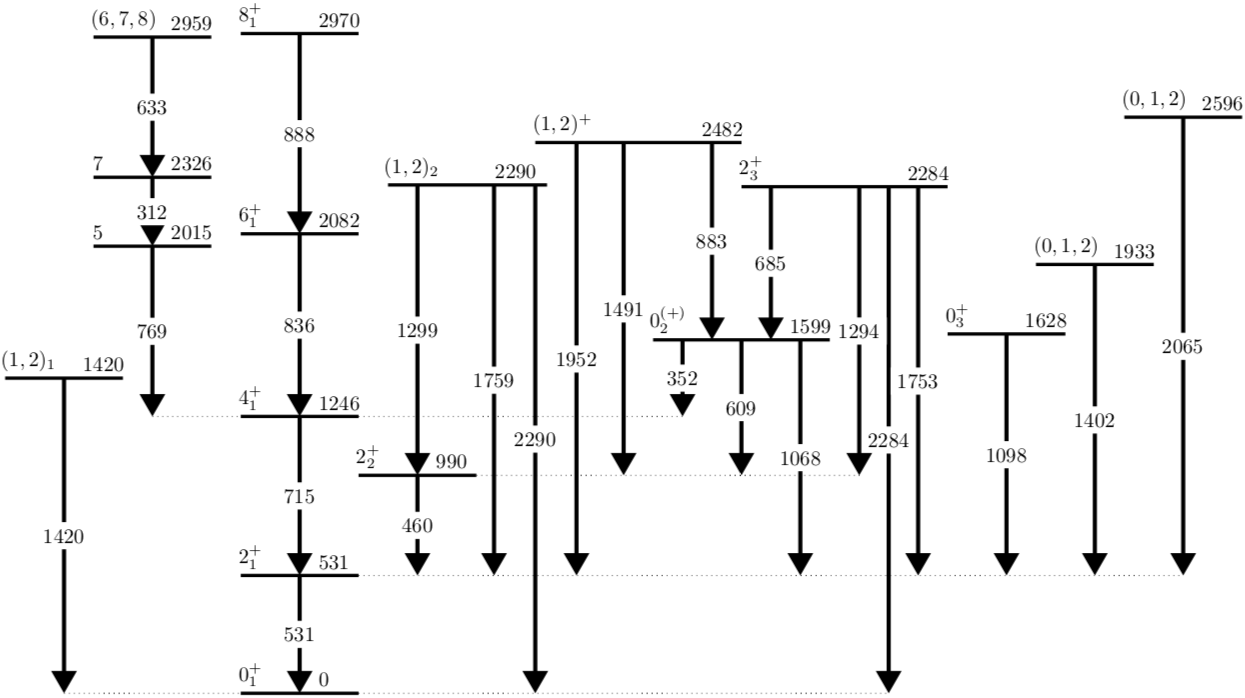
\includegraphics[width=\textwidth]{Images/Level-scheme-140Sm-v2.png}
	\caption{Level scheme for \Sm\ based on \cite{Klintefjord, NNDC-levels}. 
	The energies for the levels and transitions are in keV and are rounded to the nearest integer.
	See text for more information.}
	\label{fig:levels}
\end{figure}

In addition to all the transitions visible in the \ga\ spectrum in \autoref{fig:gam_dcB}, it is expected to see a transition from an unknown $3^+$ state which should transition into the $2_2^+$ state \cite{Klintefjord2016, Samorajczyk2015}.
The $3^+$ state is expected as a member of the \ga-vibrational band, which is expected to be built on the $2_2^+$ state.
Theory predicts that the $3^+$ state should roughly be around 1900 keV.
In the spectrum of \autoref{fig:gam_dcB}, there is no obvious candidate for a transition from the expected $3^+$ state.
However, the width of the $6_1^+ \rightarrow 4_1^+$ transition at 836 keV is slightly wider than the other transitions. 
\ga-\ga\ coincidences can be used to investigate if the peak at 836 keV is composed of more than one transition. 
\autoref{fig:check_state} shows a coincidence spectra of gates on the left and right flank of the 836 keV peak.
The transition at approximately 844 keV is a very good candidate for the missing member of the \ga-band. 
This new transition and new state will really help to clarify the role of triaxiality.
The sum-peak of the assumed $3^+$ and the $2_2^+$ state is 1834 keV, which is close to the rough estimate of around 1900 keV.
We cannot expect to see a transition down to the ground state from 1834 keV, since it would have been a M3 transition. 
%In principle, there can be a transition from $3^+$ to $4^+$, but there was no sign of this either.

There is a possible new peak around 1860 keV in \autoref{fig:gam_dcB}. 
None of the sum-peaks from \autoref{fig:levels} add up to this energy level. 
\textcolor{red}{Kan det være summen av flere forskjellige overganger, som ikke er åpenbare i level scheme? Som f.eks. 888 ($8_1^+ \rightarrow 6_1^+$) + 460 ($2_2^+ \rightarrow 2_1^+$) + 531 (($2_1^+ \rightarrow 0_1^+$)) = 1879 keV. 888 og 531 er åpenbare, men er det også åpenbart at 460 kommer samtidig? 836 + 460 + 531 = 1827.}

\begin{figure}[htb]
	\centering
	\includegraphics[width=\textwidth]{Images/check_state.png}
	\caption{\textbf{(a)} A gate on the left flank of the broad peak at 836 keV, showing coincidences with the 715 keV ($4_1^+ \rightarrow 2_1^+$) and 531 keV ($2_1^+ \rightarrow 0_1^+$) transitions.
	%yrast cascade.
	\textbf{(b)} Gate on the right flank of the 836 keV peak, showing coincidences with the 460 keV ($2_2^+ \rightarrow 2_1^+$) and 531 keV ($2_1^+ \rightarrow 0_1^+$) transitions.
	\textbf{(c)} In red, a gate on the 715 keV ($4_1^+ \rightarrow 2_1^+$) transition, showing the 836 keV ($6_1^+ \rightarrow 4_1^+$) and 888 keV ($8_1^+ \rightarrow 6_1^+$) transitions. In blue, a gate on the 460 keV ($2_2^+ \rightarrow 2_1^+$) transition, showing a new transition at 844 keV, presumably from the $3^+$ state belonging to the \ga-vibrational band.
	}
	\label{fig:check_state}
\end{figure}

\autoref{fig:gg_dcB} displays the \ga\ga-matrix Doppler corrected for the beam.
The diagonal lines below 600 keV, comes from the Compton continuum. \textcolor{red}{Is this correct?} 
Here, we see defined lines where the constituents of the ground state band is as mentioned before (531 keV, 715 keV, 836 keV and a slim 888 keV line), in addition to the 460 keV line. 
The 836 keV line is quite broad.

\begin{figure}[htb!]
	\centering
	% GammaPlot.cpp
	% gg_matrix_dcB("setup_Coulex.txt", "d")
	\includegraphics[width=\textwidth]{../Plots/plotting/gg_dcB.png}
	\caption{\ga-\ga\ matrix Doppler corrected for beam (\Sm).}
	\label{fig:gg_dcB}
\end{figure}


In the previous experiment at ISOLDE, IS495 in 2012, three excited states of \Sm\ were populated, the first (531 keV) and second (990 keV) excited $2^+$ states, in addition to the first $4^+$ (1246 keV) state.
The \ga-ray intensities for the specified low-lying states was measured from 5 separate ranges of CM scattering angles, Doppler corrected for the \Sm\ projectiles. 
These intensities are used to obtain the reduced transition probabilities, i.e. the $B(E2)$ values of the specified low-lying states \cite{Klintefjord2015, Klintefjord2016, BelloGarrote2015}.

From the present experiment at ISOLDE, IS558 in 2017, excited sates up to $8^+$ were populated. 
New measurements of the \ga-ray intensities can be performed for 23 separate ranges of CM scattering angles, Doppler corrected for the \Sm\ projectiles, specified by \autoref{tab:scattering}. 
\autoref{fig:projections} displays the coverage of the CM scattering angle range $\theta_b^{'} \in [36.6^\circ, 136.0^\circ]$ of the beam.
It is split into 6 parts as an example of the quality of the new measurement, but this can further be split into 23 parts.
The 23 separate angle ranges will give much more data points compared to the former 5 separate angle ranges.
By analyzing the 23 CM angle ranges, the precision of the previous measurements of the three $B(E2)$ values will certainly be improved, in addition to measuring many unknown $B(E2)$ values.
The reduced transition probabilites, i.e. $B(E2)$, are relatively strong in the ground state band. 
\textcolor{red}{Må jeg si hvordan disse er koblet mot matrise-elementene eller kan jeg la være å si det? Hvis jeg må forklare det, hvordan var det igjen? Hvis jeg ikke må forklare det, kan vi snakke om dette senere.}


\begin{figure}[htb!]
	\centering
	\begin{subfigure}[t]{0.49\textwidth}
		\centering
		\includegraphics[width=\textwidth]{../Plots/plotting/Projections-combined/B_dcB_x-ProjY_2-4_combined}
		\caption{}
		%\label{fig:???}
	\end{subfigure}
	\hfill
	\begin{subfigure}[t]{0.49\textwidth}
		\centering
		\includegraphics[width=\textwidth]{../Plots/plotting/Projections-combined/B_dcB_x-ProjY_5-8_combined}
		\caption{}
		%\label{fig:???}
	\end{subfigure}
	\begin{subfigure}[t]{0.49\textwidth}
		\centering
		\includegraphics[width=\textwidth]{../Plots/plotting/Projections-combined/B_dcB_x-ProjY_9-12_combined}
		\caption{}
		%\label{fig:???}
	\end{subfigure}
	\hfill
	\begin{subfigure}[t]{0.49\textwidth}
		\centering
		\includegraphics[width=\textwidth]{../Plots/plotting/Projections-combined/B_dcB_x-ProjY_13-16_combined}
		\caption{}
		%\label{fig:???}
	\end{subfigure}
	\begin{subfigure}[t]{0.49\textwidth}
		\centering
		\includegraphics[width=\textwidth]{../Plots/plotting/Projections-combined/T_dcB_x-ProjY_5-8_combined.png}
		\caption{}
		%\label{fig:???}
	\end{subfigure}
	\hfill
	\begin{subfigure}[t]{0.49\textwidth}
		\centering
		\includegraphics[width=\textwidth]{../Plots/plotting/Projections-combined/T_dcB_x-ProjY_2-4_combined.png}
		\caption{}
		%\label{fig:???}
	\end{subfigure}
	\caption{\textbf{(a)-(d)} shows when the beam particle hits the CD with the LAB angle as specified in the plot title, while \textbf{(e)-(f)} shows when the target hits the CD with the LAB angle as specified in the plot title. T is for target and B is for beam. Combined they cover the angle range $\theta_b^{'} \in [36.6^\circ, 136.0^\circ]$ of the beam in the CM frame.}
	\label{fig:projections}
\end{figure}



\bigskip

% \cite{Klintefjord2015, Samorajczyk2015, Klintefjord2016}
% \cite{BelloGarrote2015}

%\autoref{fig:gam_dcB}
%\autoref{fig:levels}
%\autoref{tab:gamma_trans}




% ----------------------------------------------------------------------------------------------------------------------% ----------------------------------------------------------------------------------------------------------------------

\chapter{Summary and outlook}
\epigraph{\textit{"Nothing happens until something moves."}}{\textit{– Albert Einstein}}


Future work: Better calibration of particle detectors and \ga\ detectors (online not perfect). Take into account the shape of the peaks $\implies$ calibrate the particle detectors manually.. Takes a lot of time! But maybe less than trying to fit all in a script? If someone only knew and told this story...

Use a second opinion on the simulation, maybe try LISE++ or some other simulation program to get the centroids?
Maybe \texttt{kinsim3} uses too much energy loss in CD? 
If you are using only the Pb and Sm for calibration, and then applying that calibration back to the data, then it should matter if the absolute energies are correct. 
This is an internal calibration, so that would simply mean that the peaks would have the wrong energy, but they should still be aligned on the front and back.


\bigskip

Geometry:
For the geometry, I am not sure exactly what the best set of angles are. You should produce some spectra to analyse before determining this. In the output file of CLXAna you will find a histogram called B\_dcB\_cid, which is the Doppler corrected spectra vs. each detector. The peak energies should of course be constant as a function of detector number, if they vary, then the angles need to be improved.


\bigskip


In the Sm data, the issue came in determining the peak centroid or maximum for the experimental data. 
The peak shape is a convolution of many effects; intrinsic resolution of the detector, the beam energy width, straggling in the target, interaction points in the target, angular width of the detector strip, etc. 
While the simulation tries to include all these things, it was found that the peak shapes were not exactly the same. 
It might be worthwhile spending a bit of time to play with the parameters and try to get the peak shape as similar as possible. 
At that point, maybe use a certain feature of the peak, such as the maximum, or the highest energy edge. 
Or, honestly, it might be better to simply hover the mouse over the correct "feature" of the peak and position it by eye, be it the centroid or the maximum.
Then the same feature in the corresponding simulated spectrum can be analyzed.
The maximum of the peak on the high energy side is not the center of the peak, but roughly equivalent to the maximum. 
It can be imagined as fitting a Gaussian to the right-hand side, the high-energy side only, as this would be roughly where the centroid is. 


\bigskip

Efficiency calibration ++

\bigskip

\textcolor{red}{Fra oppgaveteksten:} \newline
determine Coulomb excitation yields. These yields will then, in a second step, be compared to theoretical calculations and transition probabilities and quadrupole moments will be extracted using chi-square minimization procedures.


GOSIA and GOSIA2 analysis?

\url{https://www.pas.rochester.edu/~cline/Gosia/Gosia_Manual_20110609.pdf}

\bigskip

Look for an updated version of \textsl{MiniballCoulexSort} and ask Dr. Liam Gaffney if there are any new considerations of how to use it with data from 2017.

\bigskip

Coulomb excitation yields. These yields will then, in a second step, be compared to theoretical calculations and transition probabilities and quadrupole moments will be extracted using chi-square minimization procedures.

\bigskip

Expect to measure transition probabilities $B(E2)$ and quadrupole moment (nuclear deformation). 

\bigskip

the experiment can help figure out if the triaxial deformation is rigid or soft.

\bigskip

Very pure beam (\textcolor{red}{did we have statistics of this?}) - resultat til avhandling. sjekk etter doppler-korrigering. Nd-contaminasjon? i så fall veldig lite, 1-2 prosent? Beam composition, laser on/off.

\textcolor{Magenta}{Tilbakemelding: \newline
we would have to look at the \ga-spectra to identify any contaminants. There may be a little bit of Nd-140 in the beam, but if so, it is very little (judging from on-line spectra).}

\bigskip

we don't extract B(E2) values, and don't discuss transition strengths. To extract these is the next step

\bigskip

to get even better results and maybe see some of the low-energy transitions which disappears into the Compton continuum, do a new experiment with Compton suppression, shielded (BGO shield?) \ga\ detectors.


% NOT NEEDED
%\begin{table}[htb] 
%    \centering 
%    \caption{Known $B(E2)$ values with corresponding errors, from \cite{Klintefjord2016, BelloGarrote2015}. Here TNA (LNA) is an acronym for Target (Lifetime) Normalization Approach, while LM is an acronym for Lifetime Measurement.}
%	% Data for the B(E2) table
\begin{tabular}{ccccc}
\hline
        &         & \multicolumn{3}{c}{$B(E2; I_i \rightarrow I_f)$ [e$^2$b$^2$]} \\
$I_i$   & $I_f$   & TNA $\cite{Klintefjord2016}$ & LNA $\cite{Klintefjord2016}$ & LM $\cite{BelloGarrote2015}$ \\
\hline
$2_1^+$ & $0_1^+$ & 0.25$_{-0.01}^{+0.02}$       & 0.21$_{-0.01}^{+0.02}$       & 0.216(15)                    \\
$4_1^+$ & $2_1^+$ & 0.30$_{-0.02}^{+0.02}$       & 0.29$_{-0.02}^{+0.02}$       &                              \\
$2_2^+$ & $2_1^+$ & 0.35$_{-0.05}^{+0.05}$       & 0.35$_{-0.05}^{+0.04}$       &                              \\
\hline
\end{tabular}
%	\label{tab:BE2}
%\end{table}


% ----------------------------------------------------------------------------------------------------------------------% ----------------------------------------------------------------------------------------------------------------------




% ----------------------------------------------------------------------------------------------------------------------% ----------------------------------------------------------------------------------------------------------------------

\begin{appendices}

\chapter{Acronyms and abbreviations}

\begin{table}[ht] 
	\centering 
	%\caption{Table of acronyms and abbreviations.}
	% Data for the Acronyms and abbreviations table
\begin{tabular}{ll}
    \hline
    ADC         &  Analog to Digital Converter                                \\
    bash        &  Bourne-Again SHell                                         \\
    CERN        &  European Council for Nuclear Research                      \\ 
                &  (in French: Conseil Européen pour la Recherche Nucléaire)  \\
    CD          &  Compact Disc                                               \\
    COULEX      &  COULomb EXcitation                                         \\
    DAQ         &  Data AcQuisition                                           \\
    DGF         &  Digital Gamma Finder                                       \\
    DSSSD       &  Double Sided Silicon Strip Detector (also known as CD)     \\
    GPS         &  General Purpose Separator                                  \\
    HRS         &  High Resolution Separator                                  \\
    HIE-ISOLDE  &  High Intensity and Energy upgrade at ISOLDE                \\
    HPGe        &  High Purity Germanium                                      \\
    ISOL        &  Isotope Separator On Line                                  \\
    ISOLDE      &  ISOL DEvice                                                \\
    LINAC       &  LINear ACcelerator                                         \\
    MBS         &  Multi Branch System                                        \\
    MED         &  MBS Event Data (also known as Miniball Event Data)         \\
    MAR\belowbaseline[-2pt]{a}B\stackinset{l}{3pt}{b}{-3pt}{O}{O}\,U     
                &  MBS And ROOT Based Online/Offline Utility                  \\
    PSB         &  Proton Synchrotron Booster                                 \\
    REX         &  Radioactive beam EXperiment                                \\
    EBIS        &  Electron Beam Ion Source                                   \\
    REXEBIS     &  Radioactive beam EXperiment Electron Beam Ion Source       \\
    REXTRAP     &  Radioactive beam EXperiment TRAP                           \\
    REX-ISOLDE  &  Radioactive beam EXperiment at ISOLDE                      \\
    RIB         &  Radioactive Ion Beam                                       \\
    RILIS       &  Resonance Ionization Laser Ion Source                      \\
    SRIM        &  Stopping and Range of Ions in Matter                       \\
    TDC         &  Time to Digital Converter                                  \\
    \hline
\end{tabular}
\label{tab:acro}

	\label{tab:acro}
\end{table}


% ----------------------------------------------------------------------------------------------------------------------% ----------------------------------------------------------------------------------------------------------------------

\chapter{Two-particle elastic collision}\label{ch:scattering}
\section{Laboratory (LAB) frame of reference}\label{sec:LAB}
The angles of the two-particle collision in the laboratory frame from \autoref{fig:scattering} is calculated in this section. 
A general approach is used to make it easier to hold track of the parameters. 
From the figure we can express the velocities as
\begin{align}\label{eq:2p-LAB-collision}
\begin{split}
	 \boldsymbol{u} &= \boldsymbol{u}_1 = u \boldsymbol{\hat{x}}  \\
	 \boldsymbol{u}_2 &= 0  \\
	 \boldsymbol{v}_b &= \boldsymbol{v}_1 = v_1 (\cos \theta \boldsymbol{\hat{x}} + \sin \theta \boldsymbol{\hat{y}})  \\
	\boldsymbol{v}_t &= \boldsymbol{v}_2 = v_2 (\cos \varphi \boldsymbol{\hat{x}} - \sin \varphi \boldsymbol{\hat{y}})
\end{split}
\end{align}
where $\boldsymbol{u}_1$ and $\boldsymbol{v}_1$ is the initial and final velocity of the projectile $m_b = m_1$ respectively, and $\boldsymbol{u}_2$ and $\boldsymbol{v}_2$ is the initial and final velocity of the target $m_t = m_2$ respectively. The angles $\theta_b = \theta$ and $\theta_t = \varphi$ are the projectile and target angle respectively. We also introduce a ratio of the projectile mass to the target mass, $\alpha = m_1/m_2$.

Conservation of momentum gives
\begin{align*}%\label{eq:comom}
	m_1 \boldsymbol{u}_1 &= m_1 \boldsymbol{v}_1 + m_2 \boldsymbol{v}_2
\end{align*}
which in $x$-direction can be expressed as
\begin{align}\label{eq:comx}
	m_1 u &= m_1 v_1 \cos \theta + m_2 v_2 \cos \varphi  \nonumber\\
	m_1 (u - v_1 \cos \theta) &= m_2 v_2 \cos \varphi  \nonumber\\
	\frac{m_1}{m_2} (u - v_1 \cos \theta) &= v_2 \cos \varphi  \nonumber\\
	\alpha (u - v_1 \cos \theta) &= v_2 \cos \varphi
\end{align}
and in $y$-direction can be expressed as
\begin{align}\label{eq:comy}
	0 &= m_1 v_1 \sin \theta - m_2 v_2 \sin \varphi \nonumber\\
	m_1 v_1 \sin \theta &= m_2 v_2 \sin \varphi \nonumber\\
	\frac{m_1}{m_2} v_1 \sin \theta &= v_2 \sin \varphi \nonumber\\
	\alpha v_1 \sin \theta &= v_2 \sin \varphi
\end{align}

Conservation of energy gives
\begin{align}\label{eq:coe}
	\tfrac{1}{2} m_1 \boldsymbol{u}_1^2 &= \tfrac{1}{2} m_1 \boldsymbol{v}_1^2 + \tfrac{1}{2} m_2 \boldsymbol{v}_2^2 \nonumber\\
	\tfrac{1}{2} m_1 (u^2 - v_1^2) &= \tfrac{1}{2} m_2 v_2^2 \nonumber\\
	\frac{m_1}{m_2} (u^2 - v_1^2) &= v_2^2 \nonumber\\
	\alpha (u^2 - v_1^2) &= v_2^2
\end{align}

We now have three equations, \autoref{eq:comx} - \autoref{eq:coe}, with four unknown quantities ($v_1, \theta, v_2, \varphi$). 
Using the target angle $\varphi$ as an independent variable, we can find expressions for the other three variables. 

Squaring \autoref{eq:comx} 
\begin{align*}%\label{eq:c}
	\alpha^2 (u - v_1 \cos \theta)^2 &= v_2^2 \cos^2 \varphi  \\
	\alpha^2 (u^2 - 2uv_1 \cos \theta + v_1^2 \cos^2 \theta) &= v_2^2 \cos^2 \varphi
\end{align*}
and \autoref{eq:comy}
\begin{align*}%\label{eq:c}
	\alpha^2 v_1^2 \sin^2 \theta &= v_2^2 \sin^2 \varphi
\end{align*}
and adding them together gives
\begin{align}\label{eq:av}
	\alpha^2 (u^2 - 2uv_1 \cos \theta + v_1^2 \cos^2 \theta + v_1^2 \sin^2 \theta) &= v_2^2 (\cos^2 \varphi + \sin^2 \varphi)  \nonumber\\
	\alpha^2 (u^2 - 2uv_1 \cos \theta + v_1^2) &= v_2^2  \nonumber\\
	\alpha^2 u^2 - 2\alpha^2 uv_1 \cos \theta + \alpha^2 v_1^2 &= v_2^2  \nonumber\\
	\alpha^2 v_1^2 &= -\alpha^2 u^2 + 2\alpha^2 uv_1 \cos \theta + v_2^2  \nonumber\\
	\alpha^2 v_1^2 &= -\alpha^2 u^2 + 2\alpha u (\alpha v_1 \cos \theta) + v_2^2
\end{align}
From \autoref{eq:comx} we have
\begin{align}\label{eq:comx2}
	\alpha (u - v_1 \cos \theta) &= v_2 \cos \varphi  \nonumber\\
	\alpha u - \alpha v_1 \cos \theta &= v_2 \cos \varphi  \nonumber\\
	\alpha v_1 \cos \theta &= \alpha u - v_2 \cos \varphi
\end{align}
Substituting for \autoref{eq:comx2} into \autoref{eq:av} we get
\begin{align}\label{eq:comsq}
	\alpha^2 v_1^2 &= -\alpha^2 u^2 + 2\alpha u (\alpha u - v_2 \cos \varphi ) + v_2^2  \nonumber\\
	\alpha^2 v_1^2 &= -\alpha^2 u^2 + 2\alpha^2 u^2 - 2\alpha u v_2 \cos \varphi + v_2^2  \nonumber\\
	\alpha^2 v_1^2 &= \alpha^2 u^2 - 2\alpha u v_2 \cos \varphi + v_2^2
\end{align}
Using \autoref{eq:coe} we get
\begin{align}\label{eq:coesub}
    \left( \frac{\alpha}{\alpha} \right) \alpha (u^2 - v_1^2) &= v_2^2  \nonumber\\
    \alpha^2 (u^2 - v_1^2) &= \alpha v_2^2  \nonumber\\
	\alpha^2 u^2 - \alpha^2 v_1^2 &= \alpha v_2^2  \nonumber\\
	\alpha^2 v_1^2 &= \alpha^2 u^2 - \alpha v_2^2
\end{align}
Combining \autoref{eq:comsq} and \autoref{eq:coesub} gives
\begin{align}\label{eq:comcoe}
    \alpha^2 u^2 - 2\alpha u v_2 \cos \varphi + v_2^2 &= \alpha^2 u^2 - \alpha v_2^2  \nonumber\\
    v_2^2 + \alpha v_2^2 &= 2\alpha u v_2 \cos \varphi  \nonumber\\
    v_2^2 (1 + \alpha) &= 2\alpha u v_2 \cos \varphi  \nonumber\\
    v_2 &= 2 \left( \frac{\alpha}{1 + \alpha} \right) u \cos \varphi 
\end{align}
Substituting \autoref{eq:comcoe} into \autoref{eq:coesub} we get
\begin{align}\label{eq:coesubsub}
    \alpha^2 v_1^2 &= \alpha^2 u^2 - \alpha \left( 2 \left( \frac{\alpha}{1 + \alpha} \right) u \cos \varphi  \right)^2  \nonumber\\
    v_1^2 &= u^2 - \frac{1}{\alpha} \left( 4 \left( \frac{\alpha^2}{(1 + \alpha)^2} \right) u^2 \cos^2 \varphi  \right)  \nonumber\\
    v_1^2 &= u^2 \left(1 - 4 \left( \frac{\alpha}{(1 + \alpha)^2} \right) \cos^2 \varphi  \right)  \nonumber\\
    v_1 &= u \sqrt{1 - 4 \frac{\alpha}{M} \cos^2 \varphi}
\end{align}
where $\alpha/M = \alpha/(1 + \alpha)^2$. 
The ratio of \autoref{eq:comy} and \autoref{eq:comx2} gives
\begin{align}\label{eq:comxy}
	\frac{\alpha v_1 \sin \theta}{\alpha v_1 \cos \theta} &= \frac{v_2 \sin \varphi}{\alpha u - v_2 \cos \varphi}  \nonumber\\
	\tan \theta &= \frac{v_2 \sin \varphi}{\alpha u - v_2 \cos \varphi}
\end{align}
Inserting \autoref{eq:comcoe} into \autoref{eq:comxy} gives
\begin{align}\label{eq:tanBgen}
	\tan \theta &= \frac{\left( 2 \left( \frac{\alpha}{1 + \alpha} \right) u \cos \varphi  \right) \sin \varphi}{\alpha u - \left( 2 \left( \frac{\alpha}{1 + \alpha} \right) u \cos \varphi  \right) \cos \varphi}  \nonumber\\
	\tan \theta &= \frac{\alpha u \left( \frac{1}{1 + \alpha} \right) 2 \sin \varphi \cos \varphi}{\alpha u \left(1 - 2 \left( \frac{1}{1 + \alpha} \right) \cos^2 \varphi \right)}  \nonumber\\
	\tan \theta &= \frac{\sin 2\varphi}{(1 + \alpha)\left(1 - 2 \left( \frac{1}{1 + \alpha} \right) \cos^2 \varphi \right)}  \nonumber\\
	\tan \theta &= \frac{\sin 2\varphi}{1 + \alpha - 2 \cos^2 \varphi}  \nonumber\\
	\tan \theta &= \frac{\sin 2\varphi}{\alpha - (2 \cos^2 \varphi - 1)}  \nonumber\\
	\tan \theta &= \frac{\sin 2\varphi}{\alpha - \cos 2\varphi}  \nonumber\\
	\theta &= \arctan \left( \frac{\sin 2\varphi}{\alpha - \cos 2\varphi} \right)
\end{align}
Substituting back the variable names from the LAB frame in \autoref{fig:scattering} into \autoref{eq:tanBgen} gives
\begin{align}\label{eq:tanB}
	\theta_b &= \arctan \left( \frac{\sin 2\theta_t}{\alpha - \cos 2\theta_t} \right)
\end{align}


\section{Center of mass (CM) frame of reference}
Using the same approach as \autoref{sec:LAB}. 
From the CM frame in \autoref{fig:scattering} we can express the velocities as
\begin{align}\label{eq:2p-CM-collision}
\begin{split}
	 \boldsymbol{u}_1^{'} &= u_1^{'} \boldsymbol{\hat{x}} \\
	 \boldsymbol{u}_2^{'} &= u_2^{'} \boldsymbol{\hat{x}} \\
	 \boldsymbol{v}_b^{'} &= \boldsymbol{v}_1^{'} = v_1^{'} (\cos \theta^{'} \boldsymbol{\hat{x}} + \sin \theta^{'} \boldsymbol{\hat{y}}) \\
	\boldsymbol{v}_t^{'} &= \boldsymbol{v}_2^{'} = v_2^{'} (-\cos \theta^{'} \boldsymbol{\hat{x}} - \sin \theta^{'} \boldsymbol{\hat{y}}) = -v_2^{'} (\cos \theta^{'} \boldsymbol{\hat{x}} + \sin \theta^{'} \boldsymbol{\hat{y}})
\end{split}
\end{align}
where $\boldsymbol{u}_1^{'}$ and $\boldsymbol{v}_1^{'}$ is the initial and final velocity of the projectile $m_b = m_1$ respectively, and $\boldsymbol{u}_2^{'}$ and $\boldsymbol{v}_2^{'}$ is the initial and final velocity of the target $m_t = m_2$ respectively. 
The angle $\theta_b^{'} = \theta^{'}$ is the projectile angle. 

In the center of mass (CM) frame of reference, the position of the center of mass is given by
\begin{align}\label{eq:CMpos}
	\boldsymbol{R} &= \frac{m_1 \boldsymbol{r}_1 + m_2 \boldsymbol{r}_2}{m_1 + m_2}
\end{align}
and the velocity is
\begin{align}\label{eq:Vcm}
	\boldsymbol{V} &= \frac{d\boldsymbol{R}}{dt}
	= \frac{d}{dt} \left( \frac{m_1 \boldsymbol{r}_1 + m_2 \boldsymbol{r}_2}{m_1 + m_2} \right)
	= \frac{m_1 \boldsymbol{u}_1^{'} + m_2 \boldsymbol{u}_2^{'}}{m_1 + m_2}
\end{align}
At the origin of the CM frame, $\boldsymbol{R} = 0$, which implies $\boldsymbol{V} = 0$. 
The total momentum before the collision is
\begin{align}\label{eq:ucm}
	m_1 \boldsymbol{u}_1^{'} + m_2 \boldsymbol{u}_2^{'} &= 0  \nonumber\\
	m_2 u_2^{'} &= -m_1 u_1^{'} \nonumber\\
	u_2^{'} &= - \frac{m_1}{m_2} u_1^{'} \nonumber\\
	u_2^{'} &= - \alpha u_1^{'}
\end{align}
and after the collision it is
\begin{align}\label{eq:vcm}
	m_1 \boldsymbol{v}_1^{'} + m_2 \boldsymbol{v}_2^{'} &= 0  \nonumber\\
	m_2 \boldsymbol{v}_2^{'} &= -m_1 \boldsymbol{v}_1^{'} \nonumber\\
	\boldsymbol{v}_2^{'} &= - \frac{m_1}{m_2} \boldsymbol{v}_1^{'} \nonumber\\
	\boldsymbol{v}_2^{'} &= - \alpha \boldsymbol{v}_1^{'} \nonumber\\
	-v_2^{'} (\cos \theta^{'} \boldsymbol{\hat{x}} + \sin \theta^{'} \boldsymbol{\hat{y}}) &= - \alpha v_1^{'} (\cos \theta^{'} \boldsymbol{\hat{x}} + \sin \theta^{'} \boldsymbol{\hat{y}}) \nonumber\\
	v_2^{'} &= \alpha v_1^{'}
\end{align}
Conservation of energy gives
\begin{align}\label{eq:coecm}
	\tfrac{1}{2} m_1 u_1^{'2} + \tfrac{1}{2} m_2 u_2^{'2} &= \tfrac{1}{2} m_1 v_1^{'2} + \tfrac{1}{2} m_2 v_2^{'2} \nonumber\\
	m_1 u_1^{'2} + m_2 u_2^{'2} &= m_1 v_1^{'2} + m_2 v_2^{'2}
\end{align}
Substituting \autoref{eq:ucm} and \autoref{eq:vcm} into \autoref{eq:coecm} gives
\begin{align}\label{eq:u2u1}
	m_1 u_1^{'2} + m_2 (-\alpha u_1^{'})^2 &= m_1 v_1^{'2} + m_2 (\alpha v_1^{'})^2 \nonumber\\
	m_1 u_1^{'2} + \alpha^2 m_2 u_1^{'2} &= m_1 v_1^{'2} + \alpha^2 m_2 v_1^{'2} \nonumber\\
	(m_1 +\alpha^2 m_2) u_1^{'2} &= (m_1 +\alpha^2 m_2) v_1^{'2} \nonumber\\
	u_1^{'2} &= v_1^{'2} \nonumber\\
	u_1^{'} &= v_1^{'}
\end{align}
Substituting \autoref{eq:u2u1} into \autoref{eq:ucm} gives 
\begin{align}\label{eq:u2v1}
	u_2^{'} &= - \alpha v_1^{'}
\end{align}


\section{Connection between the LAB frame and the CM frame}
Galilean transformations describes the relationship between the LAB frame and the CM frame
\begin{align*}
	 x^{'} &= x - vt  & v_x^{'} &= v_x - V_{cm} \\
	 y^{'} &= y & v_y^{'} &= v_y \\
	 z^{'} &= z & v_z^{'} &= v_z \\
	 t^{'} &= t \\
\end{align*}

Using the same approach as \autoref{sec:LAB}. In the LAB frame of \autoref{fig:scattering}, conservation of momentum is given by
\begin{align}\label{eq:comlab}
	m_1 \boldsymbol{u}_1 + m_2 \boldsymbol{u}_2 &= m_1 \boldsymbol{v}_1 + m_2 \boldsymbol{v}_2 = (m_1 + m_2)\boldsymbol{V}
\end{align}
which can be written as
\begin{align}\label{eq:V}
	m_1 \boldsymbol{u}_1 + m_2 \boldsymbol{u}_2 &= (m_1 + m_2)\boldsymbol{V} \nonumber\\
	\boldsymbol{V} &= \frac{m_1 \boldsymbol{u}_1 + m_2 \boldsymbol{u}_2}{m_1 + m_2} & \boldsymbol{u}_2& = 0 \nonumber\\
	\boldsymbol{V} &= \frac{m_1}{m_1 + m_2} \boldsymbol{u}_1 \nonumber\\
	\boldsymbol{V} &= \frac{\alpha}{1 + \alpha} u \boldsymbol{\hat{x}} \nonumber\\
	V &= \frac{\alpha}{1 + \alpha} u
\end{align}

Using Galilean transformations, the connection between $\boldsymbol{v}_1^{'}$ and $\boldsymbol{v}_1$ is expressed as
\begin{align}\label{eq:vcmv}
	\boldsymbol{v}_1^{'} &= \boldsymbol{v}_1 - \boldsymbol{V} \nonumber\\
	\boldsymbol{v}_1 &= \boldsymbol{v}_1^{'} + \boldsymbol{V}
\end{align}
which in $x$-direction gives
\begin{align}\label{eq:vcmvx}
	v_1 \cos \theta &= v_1^{'} \cos \theta^{'} + V
\end{align}
and in $y$-direction gives
\begin{align}\label{eq:vcmvy}
	v_1 \sin \theta &= v_1^{'} \sin \theta^{'}
\end{align}
The ratio of \autoref{eq:vcmvy} and \autoref{eq:vcmvx} gives
\begin{align}\label{eq:vcmvxy}
	\frac{v_1 \sin \theta}{v_1 \cos \theta} &= \frac{v_1^{'} \sin \theta^{'}}{v_1^{'} \cos \theta^{'} + V} \nonumber\\
	\tan \theta &= \frac{\sin \theta^{'}}{\cos \theta^{'} + \frac{V}{v_1^{'}}} \nonumber\\
	\tan \theta &= \frac{\sin \theta^{'}}{\frac{V}{v_1^{'}} + \cos \theta^{'}}
\end{align}
We need to reformulate the velocity ratio. 
Substitution from \autoref{eq:u2u1} gives
\begin{align}\label{eq:Vou}
	\frac{V}{v_1^{'}} = \frac{V}{u_1^{'}}
\end{align}
Using Galilean transformation and \autoref{eq:V} we have that
\begin{align}\label{u1cm}
	\boldsymbol{u}_1^{'} &= \boldsymbol{u}_1 - \boldsymbol{V} \nonumber\\
	u_1^{'} &= u_1 - V \nonumber\\
	u_1^{'} &= u - \frac{\alpha}{1 + \alpha} u \nonumber\\
	u_1^{'} &= u \left( 1 - \frac{\alpha}{1 + \alpha} \right) \nonumber\\
	u_1^{'} &= u \left( \frac{1 + \alpha - \alpha}{1 + \alpha} \right) \nonumber\\
	u_1^{'} &= \frac{1}{1 + \alpha} u
\end{align}
Substituting \autoref{eq:V} and \autoref{u1cm} into \autoref{eq:Vou} gives
\begin{align}\label{eq:Vouea}
	\frac{V}{u_1^{'}} &= \frac{\frac{\alpha}{1 + \alpha} u}{\frac{1}{1 + \alpha} u} = \alpha
\end{align}
Substituting \autoref{eq:Vouea} into \autoref{eq:vcmvxy} gives
\begin{align}\label{eq:tanB1}
	\tan \theta &= \frac{\sin \theta^{'}}{\alpha + \cos \theta^{'}}  \nonumber\\
	\theta &= \arctan \left( \frac{\sin \theta^{'}}{\alpha + \cos \theta^{'}} \right)
\end{align}
Substituting back the variable names from the CM frame of \autoref{fig:scattering} into \autoref{eq:tanB1} gives
\begin{align}\label{eq:tanB1n}
	\theta_b &= \arctan \left( \frac{\sin \theta_b^{'}}{\alpha + \cos \theta_b^{'}} \right)
\end{align}

Using Galilean transformations, the connection between $\boldsymbol{v}_2^{'}$ and $\boldsymbol{v}_2$ is expressed as
\begin{align}\label{eq:vcmv2}
	\boldsymbol{v}_2^{'} &= \boldsymbol{v}_2 - \boldsymbol{V} \nonumber\\
	\boldsymbol{v}_2 &= \boldsymbol{v}_2^{'} + \boldsymbol{V}
\end{align}
which in $x$-direction gives
\begin{align}\label{eq:vcmvx2}
	v_2 \cos \varphi &= -v_2^{'} \cos \theta^{'} + V \nonumber\\
	v_2 \cos \varphi &= V - v_2^{'} \cos \theta^{'}
\end{align}
and in $y$-direction gives
\begin{align}\label{eq:vcmvy2}
	v_2 \sin \varphi &= v_2^{'} \sin \theta^{'}
\end{align}
The ratio of \autoref{eq:vcmvy2} and \autoref{eq:vcmvx2} gives
\begin{align}\label{eq:vcmvxy2}
	\frac{v_2 \sin \varphi}{v_2 \cos \varphi} &= \frac{v_2^{'} \sin \theta^{'}}{V - v_2^{'} \cos \theta^{'}} \nonumber\\
	\tan \varphi &= \frac{\sin \theta^{'}}{\frac{V}{v_2^{'}} - \cos \theta^{'}}
\end{align}
We need to reformulate the velocity ratio. 
Substitution from \autoref{eq:vcm} and \autoref{eq:u2u1} gives
\begin{align}\label{eq:Vou2}
	\frac{V}{v_2^{'}} &= \frac{V}{\alpha v_1^{'}} = \frac{V}{\alpha u_1^{'}}
\end{align}
Substituting \autoref{eq:Vouea} into \autoref{eq:Vou2} gives
\begin{align}\label{eq:Vouea2}
	\frac{V}{v_2^{'}} &= \frac{V}{\alpha \frac{V}{\alpha}} = 1
\end{align}
Substituting \autoref{eq:Vouea2} into \autoref{eq:vcmvxy2} gives
\begin{align}\label{eq:tanT}
	\tan \varphi &= \frac{\sin \theta^{'}}{1 - \cos \theta^{'}} = \frac{1}{\frac{1 - \cos \theta^{'}}{\sin \theta^{'}}} = \frac{1}{\tan \frac{\theta^{'}}{2}} = \cot \frac{\theta^{'}}{2} \nonumber\\
	\varphi &= \tfrac{1}{2} (\pi - \theta^{'}) ~[ \text{radians} ] = \tfrac{1}{2} (180^\circ - \theta^{'}) ~[ \text{degrees} ]
\end{align}
Substituting back the variable names from \autoref{fig:scattering} into \autoref{eq:tanT} gives
\begin{align}\label{eq:tanTgen}
	\theta_t &= \tfrac{1}{2} (\pi - \theta_b^{'}) ~[ \text{radians} ] = \tfrac{1}{2} (180^\circ - \theta_b^{'}) ~[ \text{degrees} ]
\end{align}


% ----------------------------------------------------------------------------------------------------------------------% ----------------------------------------------------------------------------------------------------------------------

\chapter{Computer setup and environment}\label{a:computer_environment}

The \textsl{MiniballCoulexSort} code does not require any a lot of computing power to run. \autoref{tab:PC} shows the computer with specifications used for the sorting and data analysis. Since the data from the experiment takes up about 60 GB, the limitation was with the SSD\footnote{The SSD (solid-state drive) is the internal storage device in the computer.}. When running the sorting and event-building programs, the space on the computer rapidly vanishes. 

\begin{table}[ht] 
	\centering 
	\caption{Computer used for sorting and data analysis.}
	\label{tab:PC}
	\begin{tabular}{ll}
		\hline
		Model & MacBook Air (13-inch, 2017) \\
		\hline
		OS              & macOS High Sierra (Version 10.13.6) \\
		Processor  &  1.8 GHz (Intel Core i5, dual core, 4 threads)  \\
						 &  Max turbo frequency: 2.90 Ghz  \\
		Memory     &  8 GB (1600 MHz DDR3)  \\
		SSD		     &  128 GB  \\
		\hline
	\end{tabular}
\end{table}

The relative path of \textsl{MiniballCoulexSort}, \texttt{kinsim3} and the ROOT framework on the computer was
\begin{lstlisting}[language=sh]
~/GitHub/Miniball/MiniballCoulexSort
~/GitHub/Miniball/kinsim
~/GitHub/ROOT-framework/build
\end{lstlisting}

\autoref{tab:paths} shows the relative path of programs, scripts and files used in this thesis. 
The settingsfile \textit{MBSettings2017\_CLX\_IS558.dat}, and calibration files \textit{IS558-online.cal} and \textit{IS558-user.cal}, used in this experiment can be found in the directory specified in the table, but when used directly with \textsl{MiniballCoulexSort} the default path is \textit{$\sim$/GitHub/Miniball/MiniballCoulexSort/config}.
The file \textit{setup\_Sm.txt} is in the table twice, this is because it is two files with the same name, one for plotting and one for fitting.

\autoref{tab:run_time} displays the run time for event building with almost all run files.

\begin{table}[htb]
    \centering
    \caption{Relative path of programs, scripts and files.}
	% Data for the Relative paths table
\begin{tabular}{ll}
    \hline
    Relative path                                          & Programs / scripts / files              \\
    \hline
    $\sim$/GitHub/Miniball/kinsim                          & \texttt{kinsim3.cc}                     \\
    $\sim$/GitHub/Miniball/MiniballCoulexSort/MedToRoot    & \texttt{MedToRoot}                      \\
    $\sim$/GitHub/Miniball/MiniballCoulexSort/TreeBuilder  & \texttt{TreeBuilder}                    \\
                                                           & \texttt{AQ4Sort}                        \\
    $\sim$/GitHub/Miniball/MiniballCoulexSort/CLXAna       & \texttt{CLXAna}                         \\
    $\sim$/GitHub/MasterThesis/Miniball-config             & \textit{MBSettings2017\_CLX\_IS558.dat} \\
                                                           & \textit{IS558-online.cal}               \\
                                                           & \textit{IS558-user.cal}                 \\
                                                           & \textit{config-IS558.dat}               \\
    $\sim$/GitHub/MasterThesis/SRIM                        & SRIM files                              \\
    $\sim$/GitHub/MasterThesis/Scripts/sorting             & \texttt{M2R.sh}                         \\
                                                           & \texttt{Q4S.sh}                         \\
                                                           & \texttt{Coulex.sh}                      \\
    $\sim$/GitHub/MasterThesis/Scripts/plotting            & \texttt{ParticlePlot.cpp}               \\
                                                           & \texttt{GammaPlot.cpp}                  \\
                                                           & \textit{setup\_Sm.txt}                  \\
    $\sim$/GitHub/MasterThesis/Scripts/calibration         & \texttt{particle-calibration.py}        \\
    $\sim$/GitHub/MasterThesis/Scripts/fitting             & \texttt{ParticleFit.cpp}                \\
                                                           & \texttt{GammaFit.cpp}                   \\
                                                           & \textit{setup\_Sm.txt}                  \\
    $\sim$/GitHub/MasterThesis/Scripts/generators          & \texttt{ADC\_generator.py}              \\
                                                           & \texttt{DGF\_generator.py}              \\
                                                           & \texttt{Geometry\_generator.py}         \\
    $\sim$/GitHub/ROOT-framework/build                     & ROOT                                    \\
    $\sim$/GitHub/ROOT-framework/build/bin                 & \texttt{hadd}                           \\
    \hline
\end{tabular}
	\label{tab:paths}
\end{table}

\begin{table}[htb] 
	\centering 
	\caption{Run time for building event trees, timed with the built in command line script \texttt{time}.}
	\label{tab:run_time}
	\begin{tabular}{ll}
		\hline
		Executable   &  Run time [min] \\
		\hline
		TreeBuilder  &  $\sim$ 45   \\
		AQ4Sort       &  $\sim$ 130  \\
		\hline
	\end{tabular}
\end{table}


% ----------------------------------------------------------------------------------------------------------------------% ----------------------------------------------------------------------------------------------------------------------


\chapter{MiniballCoulexSort and ROOT}\label{ch:MBCS_ROOT}

\section{Connecting MiniballCoulexSort with ROOT}
To connect MiniballCoulexSort with ROOT you need them to share their libraries with each other. This is done with a dynamic loader, which you can find out more about here \cite{ROOTdynLoader}. 

You have to make a \textit{.rootrc} file in your home folder on your computer. In the \textit{.rootrc} file you want to write something like this 
\begin{lstlisting}[language=]
Unix.*.Root.DynamicPath:    .:</Users/trondwj/GitHub/ROOT-framework/build/lib>:/Users/trondwj/GitHub/Miniball/MiniballCoulexSort/lib:
\end{lstlisting}
This should all be in one line. The first part is to tell the system to use the dynamic loader of ROOT to connect the given paths that follow. In my case the lib folder of the ROOT install was at 
\begin{lstlisting}[language=]
/Users/trondwj/GitHub/ROOT-framework/build/lib
\end{lstlisting}
and the lib folder of the \textsl{MiniballCoulexSort} was at
\begin{lstlisting}[language=]
/Users/trondwj/GitHub/Miniball/MiniballCoulexSort/lib
\end{lstlisting}
These paths are totally individual, and you will probably not have it in the same place. Therefore these paths must be changed to fit your system. 

After making the file you either have restart the terminal or you can source the file by writing this in the terminal
\begin{lstlisting}[language=sh]
$ source ~/.rootrc
\end{lstlisting}


\section{Running ROOT and MiniballCoulexSort from anywhere in the terminal}
To run ROOT or the different scripts of \textsl{MiniballCoulexSort} anywhere in the terminal, you have to edit your \textit{.bash\_profile} file [\textit{.bash\_profile} on MacOS, \textit{.bashrc} on Linux]. In the \textit{.bash\_profile} the following commands were used 
\begin{lstlisting}[language=sh]
# Run ROOT from anywhere
export ROOTSYS=$HOME/GitHub/ROOT-framework/build
export PATH=$ROOTSYS/lib:$PATH
export PATH=$ROOTSYS/bin:$PATH
export DYLD_LIBRARY_PATH=$ROOTSYS/lib:$DYLD_LIBRARY_PATH

# Run MiniballCoulexSort from anywhere
export DYLD_LIBRARY_PATH=$HOME/GitHub/Miniball/MiniballCoulexSort/lib:$DYLD_LIBRARY_PATH
export PATH=$HOME/GitHub/Miniball/MiniballCoulexSort/lib:$PATH
export PATH=$HOME/GitHub/Miniball/MiniballCoulexSort/bin:$PATH
\end{lstlisting}
The DYLD\_LIBRARY\_PATH is used on Mac only. On other systems, use \newline LD\_LIBRARY\_PATH instead. You need to locate the \textit{lib} and \textit{bin} folders for both ROOT and \textsl{MiniballCoulexSort} and change them to fit your system, and in addition you need the build folder of your ROOT install.


\section{CLXAna}\label{sec:CLXAna}

\subsection{Input parameters}
All input parameters for \texttt{CLXAna} are stated in the GitHub repository of \textsl{MiniballCoulexSort}, but they are not explained in detail. 
From private communications with Dr. Liam Gaffney, the purpose of several input parameters have been clarified. 
The compilation parameters may be summarized as:
\begin{description}[align=left]
	\item [-c] The configuration file is a file that contains all of the input parameters, except "-cut", in order to not type the parameters into the command line each time.
	\item [-cut] The cut file  is a root file containing the graphical cuts on the kinematics from the particle histogram, "part" in the output file of \texttt{CLXAna}. 
	This is the only file path that is not possible to put into the configuration file as stated above. 
	\newline It seems a bit weird that the input of \texttt{CLXAna} is dependent on one of its output histograms, but it is the way it is for now. 
	\item [-Ex] Excitation energy of the state that you want to perform the Doppler correction for, given in keV. This is not a significant value.
	\item [-depth] The depth of the interaction in the target in mg/cm$^2$. 
	Usually assumed to be half of the thickness of the target. 
	Different values can be tested to see if it improves the Doppler correction.
	\item [-cdoffset] The rotation of the CD detector in the $\phi$ angle, with a default value of 242.6 degrees. 
	This can be optimized, but the value is usually around the default value.
	\item [-deadlayer] The thickness of the Si dead layer in mm, with a default value of 0.0007 mm.
	\item [-spededist] Not needed for this experiment.
	\item [-bg\_frac] This value depends on the time windows defined in TreeBuilder, which means it should be -0.75 for the current version. 
	The number can also be checked by taking the ratios of the $\beta$-decay background peaks in the prompt gammas ("p") and random gammas ("r") spectra in the output file of \texttt{CLXAna}.
	This is related to the time window with respect to REXEBIS. 
	A window is defined for prompt in-beam events, and those outside of the window are sorted into the background spectra. 
	Now, a weighted fraction of the background spectrum can be subtracted from the prompt spectrum, to get rid of uncorrelated background, such as $\beta$-decay that is in random coincidence with particles. 
	The fraction needed to subtract depends on the width of the time window.
\end{description}

As mentioned in \autoref{ssec:user_cal}, one line in the output from \texttt{Q4S.sh} using \texttt{TreeBuilder} was
\begin{lstlisting}[language=]
WeightPR: 0.75
\end{lstlisting}
This value is the one supposed to be used with the \textbf{-bg\_frac} input parameter when using \texttt{CLXAna}.
Even though the WeightPR value is positive, the input parameter is supposed to be negative.  


\subsection{Graphical cuts}
In this thesis, the input parameters used with \texttt{CLXAna} is found in the \textit{config-IS558.dat} file.
The first time \texttt{CLXAna} is run, every input parameter except \textbf{-cut} needs to be provided. 
A plot of energy vs. LAB angle named "part" is needed in order to make the cut file, and this plot is found inside the \textit{.root}-file sorted by \texttt{CLXAna}.
The reason for this is that CLXAna makes a kinematic reconstruction to get the angle of the particles.
This can only be done in the last part of the sorting.
This is why we only get particles against strips from \texttt{TreeBuilder}.

There is also a plot named "part" inside the \textit{.root}-file sorted by \texttt{TreeBuilder}, but this contains energy vs. annular strip.
To make the cut file, the "part" plot from the output file of \texttt{CLXAna} needs to be opened.
It is also advised to use log scale on the $z$-axis, the draw option "colz" and to zoom into the correct area.
From this plot, graphical cuts around the beam particle and target particle events needs to be done separately. 
After making the cuts, right click and SetName to set the names to "Bcut" and "Tcut" respectively. 
Then right click and SaveAs, giving the name of a \textit{.root}-file of your choice for each cut separately. 
The key is the \textit{.root} extension so that it knows which format to use. 
In this thesis, the files were saved as \textit{Bcut.root} and \textit{Tcut.root} respectively.
The two files can be added together using a ROOT program called \texttt{hadd}, which is used like this
\begin{lstlisting}[language=]
hadd outputfile.root input_file_1.root input_file_2.root 
\end{lstlisting}

As seen in the output of the \texttt{CLXAna} run in \autoref{ssec:gamma}, the cut file \textit{outputfile.root} is provided as  
\begin{lstlisting}[language=]
outputfile.root:Bcut:Tcut
\end{lstlisting}
The \textit{:Bcut:Tcut} ending are the names of the cuts in the file. 
The first cut is the beam particles and the second is the target particles. 
These names can be chosen by the user, but they must match the names set in the graphical cuts. 

% ----------------------------------------------------------------------------------------------------------------------% ----------------------------------------------------------------------------------------------------------------------

\chapter{Signal cable wiring of the CD and naming of histograms}

\begin{table}[ht] 
	\centering 
	\caption{Signal cable wiring of the CD into the ADCs for Coulomb excitation experiments.
	The first two columns show the range of the possible numbers of the ADC and the quadrants.}
	% Data for the ADC table
\caption{ADC}
\label{tab:ADC}
\begin{tabular}{cccc}
\hline
ADC    & Quadrant & Channel &  \shortstack{Front ring [F] or \\ back strip [B]} \\
\hline
0 - 3  &  1 - 4   &  0      &  F                    		   					\\
0 - 3  &  1 - 4   &  1      &  F                    		   					\\
0 - 3  &  1 - 4   &  2      &  F                    		   					\\
0 - 3  &  1 - 4   &  3      &  F                    		   					\\
0 - 3  &  1 - 4   &  4      &  F                    		   					\\
0 - 3  &  1 - 4   &  5      &  F                    		   					\\
0 - 3  &  1 - 4   &  6      &  F                    		   					\\
0 - 3  &  1 - 4   &  7      &  F                    		   					\\
0 - 3  &  1 - 4   &  8      &  F                    		   					\\
0 - 3  &  1 - 4   &  9      &  F                    		   					\\
0 - 3  &  1 - 4   &  10     &  F                    		   					\\
0 - 3  &  1 - 4   &  11     &  F                    		   					\\
0 - 3  &  1 - 4   &  12     &  F                    		   					\\
0 - 3  &  1 - 4   &  13     &  F                    		   					\\
0 - 3  &  1 - 4   &  14     &  F                    		   					\\
0 - 3  &  1 - 4   &  15     &  F                    		   					\\
0 - 3  &  1 - 4   &  16     &  B                    		   					\\
0 - 3  &  1 - 4   &  17     &  B                    		   					\\
0 - 3  &  1 - 4   &  18     &  B                    		   					\\
0 - 3  &  1 - 4   &  19     &  B                    		   					\\
0 - 3  &  1 - 4   &  20     &  B                    		   					\\
0 - 3  &  1 - 4   &  21     &  B                    		   					\\
0 - 3  &  1 - 4   &  22     &  B                    		   					\\
0 - 3  &  1 - 4   &  23     &  B                    		   					\\
0 - 3  &  1 - 4   &  24     &  B                    		   					\\
0 - 3  &  1 - 4   &  25     &  B                    		   					\\
0 - 3  &  1 - 4   &  26     &  B                    		   					\\
0 - 3  &  1 - 4   &  27     &  B                    		   					\\
0 - 3  &          &  28     &  Empty                		   					\\
0 - 3  &          &  29     &  Empty                		   					\\
0 - 3  &          &  30     &  Empty                		   					\\
0 - 3  &  1 - 4   &  31     &  PAD                  		   					\\
  4    &          &  0      &  Ionization Chamber   		   					\\
  4    &          &  1      &  Ionization Chamber   		   					\\
\hline
\end{tabular}

	\label{tab:ADC}
\end{table}


\begin{table}[ht] 
	\centering 
	\caption{The naming and counting convention chosen for the CD with the corresponding naming of histograms from \texttt{TreeBuilder} and \texttt{AQ4Sort}.}
	% Data for the TreeBuilder vs AQ4Sort table
\caption{TreeBuilder vs AQ4Sort.}
\label{tab:TBvsAQ4}
\begin{tabular}{cccc}
\hline
Quadrant  &  Front ring or back strip  &  TreeBuilder  &  AQ4Sort      \\
\hline
1         &  Front ring 15             &  adc\_0\_0    &  fE\_Q1\_f1   \\
1         &  Front ring 14             &  adc\_0\_1    &  fE\_Q1\_f2   \\
1         &  Front ring 13             &  adc\_0\_2    &  fE\_Q1\_f3   \\
$\vdots$  &  $\vdots$                  &  $\vdots$     &  $\vdots$     \\
1         &  Front ring 1              &  adc\_0\_14   &  fE\_Q1\_f15  \\
1         &  Front ring 0              &  adc\_0\_15   &  fE\_Q1\_f16  \\
1         &  Back strip 0              &  adc\_0\_16   &  bE\_Q1\_f1   \\
1         &  Back strip 1              &  adc\_0\_17   &  bE\_Q1\_f2   \\
1         &  Back strip 2              &  adc\_0\_18   &  bE\_Q1\_f3   \\
$\vdots$  &  $\vdots$                  &  $\vdots$     &  $\vdots$     \\
1         &  Back strip 11             &  adc\_0\_26   &  bE\_Q1\_f11  \\
1         &  Back strip 12             &  adc\_0\_27   &  bE\_Q1\_f12  \\
          &                            &               &               \\
2         &  Front ring 15             &  adc\_1\_0    &  fE\_Q2\_f1   \\
$\vdots$  &  $\vdots$                  &  $\vdots$     &  $\vdots$     \\
2         &  Front ring 0              &  adc\_1\_15   &  fE\_Q2\_f16  \\
2         &  Back strip 0              &  adc\_1\_16   &  bE\_Q2\_f1   \\
$\vdots$  &  $\vdots$                  &  $\vdots$     &  $\vdots$     \\
2         &  Back strip 12             &  adc\_1\_27   &  bE\_Q2\_f12  \\
          &                            &               &               \\
3         &  Front ring 15             &  adc\_2\_0    &  fE\_Q3\_f1   \\
$\vdots$  &  $\vdots$                  &  $\vdots$     &  $\vdots$     \\
3         &  Front ring 0              &  adc\_2\_15   &  fE\_Q3\_f16  \\
3         &  Back strip 0              &  adc\_2\_16   &  bE\_Q3\_f1   \\
$\vdots$  &  $\vdots$                  &  $\vdots$     &  $\vdots$     \\
3         &  Back strip 12             &  adc\_2\_27   &  bE\_Q3\_f12  \\
          &                            &               &               \\
4         &  Front ring 15             &  adc\_3\_0    &  fE\_Q4\_f1   \\
$\vdots$  &  $\vdots$                  &  $\vdots$     &  $\vdots$     \\
4         &  Front ring 0              &  adc\_3\_15   &  fE\_Q4\_f16  \\
4         &  Back strip 0              &  adc\_3\_16   &  bE\_Q4\_f1   \\
$\vdots$  &  $\vdots$                  &  $\vdots$     &  $\vdots$     \\
4         &  Back strip 12             &  adc\_3\_27   &  bE\_Q4\_f12  \\
\hline
\end{tabular}
	\label{tab:TBvsAQ4}
\end{table}


% ----------------------------------------------------------------------------------------------------------------------% ----------------------------------------------------------------------------------------------------------------------


\chapter{kinsim3}\label{ch:cd_sim}

\section{The main function}
The main function of \texttt{kinsim3} looks like this
\begin{lstlisting}[language=c++]
kinsim3(Zb, Zt, Ab, At, thick, Eb, dEb, Ex, res, cd_dist, flat, Nevts, srim_dir)
\end{lstlisting}
where \textit{Zb} and \textit{Zt} is the proton number of the beam and target respectively, \textit{Ab} and \textit{At} is the mass number of the beam and target respectively, \textit{thick} is the target thickness in mg/cm$^2$, \textit{Eb} is the beam energy in MeV/u, \textit{dEb} is the spread of the beam energy in MeV/u, \textit{Ex} is the excitation energy in MeV, \textit{res} is the detector resolution in percent, \textit{cd\_dist} is the distance form the target to the CD in mm, \textit{flat} is the choice of a uniform or angular distribution, \textit{Nevts} is the number of particle events and \textit{srim\_dir} is the relative path of the SRIM directory.

To load \texttt{kinsim3} into ROOT, the \textbf{.L $<$filename$>$} command was used
\begin{lstlisting}[language=sh]
$ cd ~/GitHub/Miniball/kinsim
$ root
root [0] .L kinsim3.cc++
\end{lstlisting}
Adding the '$++$' at the end, forces ROOT to compile the code. 
After the simulation program was run, the file was moved and renamed with the \textbf{mv} command. 


\section{CD simulation}
On the next page, the CD simulation without Rutherford cross section is shown for each ring. 
Ring 1 is the innermost ring and ring 16 is the outermost ring. 
The plots show simulated counts vs. energy, where the first peak (lower energy) is the \Pb\ and the second peak (higher energy) is \Sm. 
%In the simulation, the Rutherford cross section was not included. 
%The relative intensity between the projectile and target peaks is therefore not the same as in the experiment, but the simulated energies are realistic.
The plots were grabbed from the \textit{.root}-file by the commands
\begin{lstlisting}[language=sh]
$ cd ~/GitHub/MasterThesis/Scripts/plotting
$ root
root [0] .L ParticlePlot.cpp++
root [1] simulation_plot("setup_Sm.txt", 0)
... <showing output from script>
\end{lstlisting}

%\texttt{kinsim3} generates pdf-files of the stopping powers automatically. 
%The rest of the plots are available inside the generated \textit{.root}-file. 
%To obtain the energy simulation for each ring, the function \textbf{simulation\_plots()} from the script \texttt{ParticlePlot.cpp} was utilized. 
%\begin{lstlisting}[language=sh]
%$ cd ~/GitHub/MasterThesis/Scripts/plotting
%$ root
%root [0] .L ParticlePlot.cpp++
%root [1] simulation_plot("setup_Sm.txt", 1)
%... <showing output from script>
%\end{lstlisting}

The next page after that shows the fitting of the CD simulation, where the red dotted curves shows the fitting of the peaks and the vertical black dotted lines shows the centroids of the peaks.

\begin{lstlisting}[language=sh]
$ cd ~/GitHub/MasterThesis/Scripts/fitting
$ root
root [0] .L ParticleFit.cpp++
root [1] simulation_fit("setup_Sm.txt")
... <showing output from script>
\end{lstlisting}

For the Si dead layer in \texttt{kinsim3}, the SRIM files must have units of MeV/mm. 
If units of MeV/cm$^2$ are used, the distance on line 359 in \texttt{kinsim3} have to be changed to the correct units. 
The correction factor is at the bottom of the SRIM file.
Line 358 and 359 in \texttt{kinsim3}, where the factor have to be changed, reads
\begin{lstlisting}[language=c++]
// Correct for dead layer loss
dist = TMath::Abs( 0.0007 / TMath::Cos( TTh ) );
\end{lstlisting}


\includepdf[pages={-}, angle=270]{../Plots/simulation/cd_sim_all.pdf}

\includepdf[pages={-}, angle=270]{../Plots/fitting/Pb_Sm_sim.pdf}


\end{appendices}

% ----------------------------------------------------------------------------------------------------------------------% ----------------------------------------------------------------------------------------------------------------------

%\bibliographystyle{unsrtnat}
\bibliographystyle{mybibstyle} %my own bibstyle to set first names to one letter + unsrtnat

\bibliography{/Users/trondwj/GitHub/MasterThesis/Thesis/References/Mendeley.bib,/Users/trondwj/GitHub/MasterThesis/Thesis/References/web_references.bib}


\end{document}